%\subsection{The Sequential Specification of OR-Set}
%\label{subsec:the sequential specification of or-set}

%The query-update rewriting of OR-set is as follows: $\gamma( \alabelshort[{\tt remove}]{a} ) = ( \alabellong[{\tt readIds}]{a}{S}{}, \alabelshort[{\tt remove}]{a,S})$.

%Each abstract state $\abstate$ is a set of tuples $(a,id)$, where $a$ is a data and $id$ is a identifier. The sequential specification $\specOrSet$ of OR-set is given by the transitions:
%\[
%  \begin{array}{rcl}
%    \abstate
%    & \specarrow{\alabellong[\mathtt{readIds}]{a}{S}{}}
%    & \abstate\
%      \begin{array}{c}
%        [\text{with}\ S = \{ (a,id)\ \vert\ (a,id) \in \abstate\}]
%      \end{array}\\
%    \abstate &
%               \specarrow{\alabelshort[\mathtt{remove}]{a,S}}
%    & \abstate \setminus S \\
%    \big(\ \abstate\ |\ \mathtt{id}\ \text{does not occur in } \abstate\ \big)
%             & \specarrow{ \alabelshort[{\tt add}]{a,id} }
%    & \abstate \cup \{ (a,\mathtt{id}) \}\\
%    \abstate
%    & \specarrow{\alabellong[\mathtt{read}]{a}{ S }{}}
%    & \abstate\
%      \begin{array}{c}
%        [\text{with}\ S = \{ a\ \vert\ \exists\ \mathtt{id}, (a,\mathtt{id}) \in \abstate \}]
%      \end{array}
%  \end{array}
%\]

%Method $\alabellong[{\tt readIds}]{a}{S}{}$ returns the set of pairs with data $a$. Method $\alabelshort[{\tt remove}]{a,S}$ removes $S$ from the abstract state. Method $\alabelshort[{\tt add}]{a,id}$ puts $\{ (a,id) \}$ into the abstract state. Method $\alabellong[{\tt read}]{}{S'}{}$ returns the contents of the or-set.




%\subsection{The Sequential Specification of List with Add-After Interface}
%\label{subsec:the sequential specification of list with add-after interface}

%Each abstract state $\abstate = (l,T)$ contains a sequence $l$ of elements of a given type and a set $T$ of elements appearing in the list. The element $l$ is the list of all input values, whether already removed or not; while $T$ stores the removed values and is used as \emph{tombstone}. The sequential specification $\specRGA$ of list with add-after interface is given with the transitions as follows:
%\[
%  \begin{array}{rcl}
%    \big(\ (l_1 \cdot a_k \cdot l_2,T\big)\ |\ a\text{ is fresh}\ \big)
%     & \specarrow{\alabelshort[\mathtt{addAfter}]{a_k,a}}
%     & (l_1 \cdot a_k \cdot a \cdot l_2,T)\\
%     \big(\ (l,T)\ |\ a_k\ \text{occurs in}\ l\ \big)
%     & \specarrow{\alabelshort[\mathtt{remove}]{a_k}}
%     & (l,T \cup \{a_k\})\\
%     (l,T)
%     & \specarrow{\alabellong[\mathtt{read}]{}{s}{}}
%     & (l,T)\
%       \left[\begin{array}{c}
%           \text{with $s$ is obtained from $l$}\\
%           \text{by removing the values in $T$}
%       \end{array}\right]
%   \end{array}
%\]

%Method $\alabelshort[\mathtt{addAfter}]{a_k,a}$ puts $a$ immediately after $a_k$ in $l$, assuming that each value is put into list at most once. Method $\alabelshort[\mathtt{remove}]{a_k}$ adds $a_k$ into $T$, hence removing $a_k$ from the list for subsequent calls to the $\mathtt{read}$ method. Thus, $\alabellong[\mathtt{read}]{}{s}{}$ returns the list content excluding any element appearing in $T$. Assume that the initial value of list is $(\circ,\emptyset)$, and $\circ$ is never removed. When the context is clear, in $\ensuremath{\tt read}$ operation, we will omit $\circ$ in return value.



\section{Implementation, Sequential Specification, and Proof of Counter}
\label{sec:implementation, sequential specification, and proof of counter}



\subsection{Counter Implementation}
\label{subsec:counter implementation}

\cite{ShapiroPBZ11} gives a operation-based counter implementation, which is shown in Listing~\ref{lst:operation-based counter}. A payload is a integer $ctr$.

\begin{figure}[t]
\begin{lstlisting}[frame=top,caption={Pseudo-code of operation-based counter},
captionpos=b,label={lst:operation-based counter}]
  payload integer ctr
  initial ctr = 0
  initial lin = @|$\epsilon$|@

  inc() :
    atSource :
      //@ lin = lin@|$\,\cdot\,$|@inc()
    downStream(inc) :
      ctr = ctr + 1

  dec() :
    atSource :
      //@ lin = lin@|$\,\cdot\,$|@dec()
    downStream(dec) :
      ctr = ctr - 1

  read() :
    //@ lin = lin@|$\,\cdot\,$|@(read()@|$\Rightarrow$|@ctr)
    return ctr
\end{lstlisting}
\end{figure}




\subsection{The Sequential Specification of Counter}
\label{subsec:the sequential specification of counter}

The sequential specification $\specCounter$ of counter is so that $\abstates = \mathbb{Z}$, that is the state will be an integer, and the transitions are given as follows:
\[
  \begin{array}[rcl]{rcl}
    k & \specarrow{\alabellong[\mathsf{inc}]{}{}} & k+1\\
    k & \specarrow{\alabellong[\mathsf{dec}]{}{}} & k-1\\
    k & \specarrow{\alabellong[\mathsf{read}]{}{k}} & k
  \end{array}
\]

Method $\alabelshort[{\tt inc}]{}$ increase the counter by $1$. Method $\alabelshort[{\tt dec}]{}$ decrease the counter by $1$. Method $\alabellong[{\tt read}]{}{k}{}$ returns the value of the counter.





\subsection{Obtain Permutations by Swapping Adjacent and Concurrent Operations}
\label{subsec:obtain permutations by swapping adjacent and concurrent operations}

Given two sequences $l_1,l_2$  such that $l_2$ is a permutation of $l_1$, let $\mathit{diff}(l_1,l_2) = \{ (a,b) \vert$ the order of $a$ and $b$ in $l_1$ is different from that of $l_2 \}$. Given a sequence $l$ and two elements $a$ and $b$ of $l$, let $\mathit{swap}(l,a,b)$ be a sequence obtained from $l$ by swapping $a$ and $b$. The following lemma states that, given two specification sequences $(\alabelset_1, \aseqord_1)$ and $(\alabelset, \aseqord_2)$ that are generated from a same history and both consistent with visibility relation, we can obtain $\aseqord_2$ from $\aseqord_1$ by several time of swapping adjacent pair of concurrent operations.

\begin{lemma}
\label{lemma:given two sequence consistent with visibility order, one can be obtained from the other}
Given a history $(\alabelset,\avisord)$ and two two specification sequences $(\alabelset_1, \aseqord_1)$ and $(\alabelset, \aseqord_2)$ that are both consistent with $\avisord$. If $\aseqord_1 \neq \aseqord_2$, then we can obtain $\aseqord_2$ from $\aseqord_1$ by several time of swapping adjacent pair of concurrent operations.
\end{lemma}

\begin {proof}

First, we need to prove that, if $\mathit{diff}(\aseqord_1,\aseqord_2) \neq \emptyset$, then, there exists $(\alabel_1,\alabel_2) \in \mathit{diff}(\aseqord_1,\aseqord_2)$, such that $\alabel_1$ and $\alabel_2$ are concurrent, and $\alabel_1$ and $\alabel_2$ are adjacent in $\aseqord_1$.

We prove this by contradiction. Assume $\mathit{diff}(\aseqord_1,\aseqord_2) \neq \emptyset$, and for each $(\alabel_1,\alabel_2) \in \mathit{diff}(\aseqord_1$, $\aseqord_2)$, we have that either $\alabel_1$ and $\alabel_2$ are not concurrent, or $\alabel_1$ and $\alabel_2$ are not adjacent in $\aseqord_1$.

Since $\mathit{diff}(\aseqord_1,\aseqord_2) \neq \emptyset$, let $(\alabel,\alabel')$ be a element of $\mathit{diff}(\aseqord_1,\aseqord_2)$, and the distance of $\alabel$ and $\alabel'$ is minimal in $\{$ the distance between $\alabel_1$ and $\alabel_2 \vert (\alabel_1,\alabel_2) \in \mathit{diff}(\aseqord_1,\aseqord_2) \}$. Let us prove that $\alabel$ and $\alabel'$ are adjacent by contradiction: If there exists $\alabel''$ between $\alabel$ and $\alabel'$. Assume that in $\aseqord_1$, $\alabel$ is before $\alabel''$, and $\alabel''$ is before $\alabel'$. By assumption, the order between $\alabel$ and $\alabel''$, and between $\alabel''$ and $\alabel'$ is the same in $\aseqord_1$ and in $\aseqord_2$. This implies that $\alabel$ is still before $\alabel'$ in $\aseqord_2$, which contradicts the fact that $(\alabel,\alabel') \in \mathit{diff}(\aseqord_1,\aseqord_2)$.

Since $\alabel$ and $\alabel'$ are adjacent and $(\alabel,\alabel') \in \mathit{diff}(\aseqord_1,\aseqord_2)$, by assumption we know that $\alabel$ and $\alabel'$ are not concurrent. Or we can say, $(\alabel,\alabel') \in \avisord \vee (\alabel',\alabel) \in \avisord$. This contradicts that both $\aseqord_1$ and $\aseqord_2$ are consistent with visibility relation. This completes the proof of the first part.

Since $\aseqord_1 \neq \aseqord_2$, we have $\mathit{diff}(\aseqord_1,\aseqord_2) \neq \emptyset$, and then, as discussed above, there exists $(\alabel,\alabel') \in \mathit{diff}(\aseqord_1,\aseqord_2)$, such that $\alabel$ and $\alabel'$ are concurrent, and $\alabel$ and $\alabel'$ are adjacent in $\aseqord_1$. Let $\aseqord_3 = \mathit{swap}(\aseqord_1,\alabel,\alabel')$. It is easy to see that $\mathit{diff}(\aseqord_1,\aseqord_2) > \mathit{diff}(\aseqord_3,\aseqord_2)$. Therefore, by several times of above process, we finally obtain $\aseqord_2$ from $\aseqord_1$ by swapping pairs of adjacent and concurrent operations. This completes the proof of this lemma. $\qed$
\end {proof}






\subsection{Proof of Operation-Based Counter}
\label{subsec:proof of operation-based counter}

The following lemma states that the operation-based counter is \crdtlinearizable{} w.r.t. $\specCounter$.

\begin{lemma}
\label{lemma:operation-based counter is correct}
The operation-based counter is \crdtlinearizable{} w.r.t $\specCounter$.
\end{lemma}

\begin {proof}
Since every operation is appended to the linearization when it executes atSource it clearly follows, the linearization order is consistent with visibility order. Then, by the causal delivery assumption, the order in which effectors are applied at a given replica is also consistent with the visibility order. Let $\alinord_1$ be the projection of linearization order into labels of effectors applied in a replica $\arep$, and $\alinord_2$ be the order of labels of effectors applied in replica $\arep$. By Lemma \ref{lemma:given two sequence consistent with visibility order, one can be obtained from the other}, $\alinord_2$ can be obtained from $\alinord_1$ by several time of swapping adjacent pair of concurrent operations. It is obvious that applying effectors of concurrent operations commute. Therefore, we know that $\mathsf{ReplicaStates}$ is an inductive invariant.

Let us prove that $\mathsf{Refinement}$ holds. We consider a refinement mapping $\refmap$ defined as the identity function. The effector produced by $\alabelshort[{\tt inc}]{}$ and the $\alabelshort[{\tt inc}]{}$ operation of the specification $\specCounter$ has exactly the same effect. The same holds for that of {\tt dec}. Applying the query {\tt read} on the replica state $\sigma$ should result in the same return value as applying the same query in the context of the specification on the same state $\refmap(\sigma)=\sigma$, which again holds trivially.

We have already prove that $\mathsf{ReplicaStates}$ is an inductive invariant and $\mathsf{Refinement}$ holds. Then, similarly as in \sectionautorefname \ref{subsec:time order of execution as linearization}, we can prove that $\mathsf{\CRDTLinshort{}}$ is an inductive invariant. $\qed$
\end {proof}








\section{Implementation and Proof of Operation-Based PN-Counter}
\label{sec:implementation and proof of operation-based PN-counter}



\subsection{PN-Counter Implementation}
\label{subsec:PN-counter implementation}

\cite{ShapiroPBZ11} introduces state-based \crdtimp{}, where an update occurs entirely at the source replica, and then propagates by transmitting the modified payload between replicas. When a replica receives an effector of modified payload, it calls method {\tt merge}, which takes the current payload and the payload in effector, and returns a new payload. \cite{ShapiroPBZ11} also shows how to obtain a operation-based \crdtimp{} from a state-based \crdtimp{}, and we draw it in Listing~\ref{lst:operation-based emulation of state-based object}. Since query operations do not change, we ignore query operations. To do a update operation $f(a)$, we compute the state-based update and perform merge in downstream. Here the precondition of downstream is empty because merge is always enabled.


\begin{minipage}[t]{1.0\linewidth}
\begin{lstlisting}[frame=top,caption={operation-based emulation of state-based object},
captionpos=b,label={lst:operation-based emulation of state-based object}]
  payload S ( the state-based payload )
  initial initial payload of S

  f(a)
    atSource :
      precondition : precondition of f(a)
      let s = atSource of f(a) in state-based
    downStream(s) :
      S = merge(S,s)
\end{lstlisting}
\end{minipage}

$\\$ $\\$

\cite{ShapiroPBZ11} gives a state-based PN-counter implementation. As discussed above, we give its operation-based version in Listing~\ref{lst:operation-based PN-counter}. Here $\alabelshort[{\tt myRep}]{}$ is a function that returns current replica identifier, and $\alabelshort[{\tt reps}]{}$ is a function that returns the number of replicas in distributed system. This implementation assumes that the number of replicas are fixed. A payload $S$ contains a integer array $P$ and a integer array $N$. $P[\arep]$ represents the number of $\alabelshort[{\tt inc}]{}$ that happens on replica $\arep$ and their effector have been applied in current replica state, while $N[\arep]$ represents the number of $\alabelshort[{\tt dec}]{}$ that happens on replica $\arep$ and their effector have been applied in current replica state. Annotation1 is an annotation for effector of {\tt inc} or {\tt dec}.


\begin{figure}[t]
\begin{lstlisting}[frame=top,caption={Pseudo-code of operation-based PN-counter},
captionpos=b,label={lst:operation-based PN-counter}]
  payload ingeter[reps()] P, ingeter[reps()] N
  initial P = [@|$0,\ldots,0$|@], N = [@|$0,\ldots,0$|@]
  initial lin = @|$\epsilon$|@

  inc()
    atSource :
      let g = myRep()
      let @|$P'$|@ = @|$P[ g: P[g] + 1]$|@
      let @|$N'$|@ = @|$N$|@
      //@ lin = lin@|$\,\cdot\,$|@inc()
    downStream(@|$(P',N')$|@) :
      @|$\forall \arep$|@, @|$P[\arep]$|@ = @|$max( P[\arep],P'[\arep] )$|@
      @|$\forall \arep$|@, @|$N[\arep]$|@ = @|$max( N[\arep],N'[\arep] )$|@
      //@ Annotation1 : @|$\forall \arep, P'[\arep]$|@ = @|$\vert \{ \alabel = \alabelshort[{\tt inc}]{}, \alabel$|@ happens on replica @|$\arep,  (\alabel,\alabel') \in \avisord \vee \alabel = \alabel', where \ \alabel'$|@ is the operation that generates this @|$(P',N')$|@ effector @|$\} \vert$|@,
      @|$N'[\arep]$|@ = @|$\vert \{ \alabel = \alabelshort[{\tt dec}]{}, \alabel$|@ happens on replica @|$\arep,  (\alabel,\alabel') \in \avisord \vee \alabel = \alabel', where \ \alabel'$|@ is the operation that generates this @|$(P',N')$|@ effector @|$\} \vert$|@,

  dec()
    atSource :
      let g = myRep()
      let @|$P'$|@ = @|$P$|@
      let @|$N'$|@ = @|$N[ g: N[g] + 1]$|@
      //@ lin = lin@|$\,\cdot\,$|@dec()
    downStream(@|$(P',N')$|@) :
      @|$\forall \arep$|@, @|$P[\arep]$|@ = @|$max( P[\arep],P'[\arep] )$|@
      @|$\forall \arep$|@, @|$N[\arep]$|@ = @|$max( N[\arep],N'[\arep] )$|@
      //@ Annotation1 : @|$\forall \arep, P'[\arep]$|@ = @|$\vert \{ \alabel = \alabelshort[{\tt inc}]{}, \alabel$|@ happens on replica @|$\arep,  (\alabel,\alabel') \in \avisord \vee \alabel = \alabel', where \ \alabel'$|@ is the operation that generates this @|$(P',N')$|@ effector @|$\} \vert$|@,
      @|$N'[\arep]$|@ = @|$\vert \{ \alabel = \alabelshort[{\tt dec}]{}, \alabel$|@ happens on replica @|$\arep,  (\alabel,\alabel') \in \avisord \vee \alabel = \alabel', where \ \alabel'$|@ is the operation that generates this @|$(P',N')$|@ effector @|$\} \vert$|@,


  read() :
    let c  = @|$\Sigma_{\arep} P[\arep]$|@ - @|$\Sigma_{\arep} N[\arep]$|@
    //@ lin = lin@|$\,\cdot\,$|@(read@|$\Rightarrow$|@c)
    return c
\end{lstlisting}
\end{figure}







\subsection{Proof of Operation-Based PN-Counter}
\label{subsec:proof of operation-based PN-counter}

We say $P_1<P_2$, if for each replica $\arep'$, we have $P_1[\arep'] \leq P_2[\arep']$, and there exists replica $\arep''$, such that $P_1[\arep''] < P_2 [\arep'']$. We say $N_1<N_2$, if for each replica $\arep'$, we have $N_1[\arep'] \leq N_2[\arep']$, and there exists replica $\arep''$, such that $N_1[\arep''] < N_2 [\arep'']$. We say $(P_1,N_1) < (P_2,N_2)$, if $(P_1 < P_2 \wedge N_1 \leq N_2) \vee (P_1 \leq P_2 \wedge N_1 < N_2)$. The following lemma states that the operation-based counter is \crdtlinearizable{} w.r.t. $\specCounter$.

\begin{lemma}
\label{lemma:operation-based PN-counter is correct}
The operation-based PN-counter is \crdtlinearizable{} w.r.t $\specCounter$.
\end{lemma}

\begin {proof}

%Let us give two facts:

%\begin{itemize}
%\setlength{\itemsep}{0.5pt}
%\item[-] $fact1$: Assume $(P_1,N_1)$ and $(P_2,N_2)$ is the effector for $\alabel_1$ and $\alabel_2$, respectively, and assume that $(\alabel_1,\alabel_2) \in \avisord$. Then, $(P_1,N_1) < (P_2,N_2)$.
%\item[-] $fact2$: Assume $(P_1,N_1)$ and $(P_2,N_2)$ is the effector for $\alabel_1$ and $\alabel_2$, respectively, and assume that $\alabel_1$ and $\alabel_2$ are concurrent. Then, $\neg ((P_1,N_1) < (P_2,N_2) \vee (P_2,N_2) < (P_1,N_1))$.
%\end{itemize}


%\noindent Proof of $fact1$: Assume $\alabel_1$ happens on replica $\arep$ and $\alabel_1 = \alabelshort[{\tt inc}]{}$. By the causal delivery assumption, we know that for each replica $\arep' \neq \arep$, $\alabel_2$ see more or equal number of {\tt inc} operations happens on replica $\arep'$ than that of $\alabel_1$, $\alabel_2$ see more or equal number of {\tt dec} operations happens on replica $\arep'$ than that of $\alabel_1$, $\alabel_2$ see more or equal number of {\tt dec} operations happens on replica $\arep$ than that of $\alabel_1$, and $\alabel_2$ see more number of {\tt inc} operations happens on replica $\arep$ than that of $\alabel_1$. By Annotation1, we know that $\forall \arep' \neq \arep$, $P_1[\arep'] \leq P_2[\arep'] \wedge N_1[\arep'] \leq N_2[\arep']$, $N_1[\arep] \leq N_2[\arep]$, and $P_1[\arep] < P_2[\arep]$. Therefore, $(P_1,N_1) < (P_2,N_2)$. The case when $\alabel_1 = \alabelshort[{\tt dec}]{}$ can be similarly proved.

%\noindent Proof of $fact2$: Let us prove that $\neg ((P_1,N_1) < (P_2,N_2) \vee (P_2,N_2) < (P_1,N_1))$ by contradiction. It is obvious that $\alabel_1$ and $\alabel_2$ happens on different replicas. Assume that $(P_1,N_1) < (P_2,N_2)$, $\alabel_1 = \alabelshort[{\tt inc}]{}$, and $\alabel_1$ happens on replica $\arep_1$. Since $(P_1,N_1) < (P_2,N_2)$, we know that for each replica $\arep'$, $P_1[\arep'] \leq P_2[\arep'] \wedge N_1[\arep'] \leq N_2[\arep']$. Especially, $P_1[\arep] \leq P_2[\arep]$. By the causal delivery assumption and Annotation1, this means $(\alabel_1,\alabel_2) \in \avisord$, contradicts the assumption that $\alabel_1$ and $\alabel_2$ are concurrent. Similarly, we can see that $\neg (V_2 < V_1)$. Therefore, $\neg (V_1 < V_2 \vee V_2 < V_1)$.  The case when $\alabel_1 = \alabelshort[{\tt dec}]{}$ can be similarly proved.

%$\newline$

%\noindent {\bf Propose Annotation2}:

Let us propose Annotation2, which is an annotation of local configuration and obviously holds in the initial global configuration.

\begin{itemize}
\setlength{\itemsep}{0.5pt}
\item[-] Annotation2: Let $(\alabelset,(P,N))$ be the local configuration of a replica. Then, for each replica $\arep$, $P[\arep]$ =  $\vert \{ \alabel \vert \alabel = \alabelshort[{\tt inc}]{}, \alabel$ happens on replica $\arep, \alabel \in \alabelset \} \vert$,
    $N[\arep]$ =  $\vert \{ \alabel \vert \alabel = \alabelshort[{\tt dec}]{}, \alabel$ happens on replica $\arep, \alabel \in \alabelset \} \vert$.
\end{itemize}

%\noindent {\bf Prove Annotation1 and Annotation2}:

Let us prove that the Annotation1 and Annotation2 are inductive invariant.

We prove by induction on executions. Obvious they hold in $\aglobalstate_0$. Assume they hold along the execution $\aglobalstate_0 \xrightarrow{}^* \aglobalstate$ and there is a new transition $\aglobalstate \xrightarrow{} \aglobalstate'$. We need to prove that they still hold in $\aglobalstate'$. We only need to consider when a replica do generator or effector of {\tt inc} and {\tt dec}:

\begin{itemize}
\setlength{\itemsep}{0.5pt}
\item[-] For case when replica $\arep$ do generator of a {\tt inc} operation $\alabel$ and then apply its effector: %Let $S=(P,N)$ and $S'=(P',N')$ be the replica state of replica $\arep$ of $\aglobalstate$ and $\aglobalstate'$, respectively.
    Let $Lc = (\alabelset,(P,N))$ and $Lc' = (\alabelset',(P',N'))$ be the local configuration of replica $\arep$ of $\aglobalstate$ and $\aglobalstate'$, respectively. Obviously, the effector of $\alabel$ is $(P',N')$.

    It is easy to see that $P'=P[r:P[r]+1]$, $N'=N$, and $\alabelset' = \alabelset \cup \{ \alabel \}$. By Annotation2 of the local configuration $Lc$, we can see that Annotation1 for effector $(P',N')$ holds, and Annotation2 for the local configuration $Lc'$ holds.

\item[-] For case when replica $\arep$ apply effector $(P_{\alabel},N_{\alabel})$ of a {\tt inc} operation $\alabel$ originated in a different replica: We only need to prove Annotation2. Let $Lc = (\alabelset,(P,N))$ and $Lc' = (\alabelset',(P',N'))$ be the local configuration of replica $\arep$ of $\aglobalstate$ and $\aglobalstate'$, respectively. Assume $\alabel$ happens on replica $\arep_{\alabel}$.
    %Let $S=(P,N)$ and $S'=(P',N')$ be the replica state of replica $\arep$ of $\aglobalstate$ and $\aglobalstate'$, respectively.

    By the causal delivery assumption, for each operation $\alabel''$, such that $\alabel''$ is visible to $\alabel$, we can see that, the effector of $\alabel''$ has already been applied in $S'$, and it is easy to see that the effector of $\alabel''$ has already been applied in $S$. It is easy to see that $\alabel'' \in \alabelset$. By Annotation1 of the effector $(P_{\alabel},N_{\alabel})$ and Annotation2 of the local configuration $Lc$, we can see that, for each replica $\arep' \neq \arep_{\alabel}$, we have $P_{\alabel}[\arep'] \leq P[\arep']$ and $N_{\alabel}[\arep'] \leq N[\arep']$.

    By the causal delivery assumption, for each operation $\alabel'$, such that $\alabel$ is visible to $\alabel'$, we can see that, the effector of $\alabel'$ has not been applied in $S'$ yet, and it is easy to see that the effector of $\alabel'$ has not been applied in $S$ yet. It is easy to see that $\alabel' \notin \alabelset$. Especially, this holds for operations happen on replica $\arep_{\alabel}$. Also, note that, the effector of $\alabel$ has not been applied in $S$ yet. It is easy to see that $\alabel \notin \alabelset$. By Annotation1 of the effector $(P_{\alabel},N_{\alabel})$ and Annotation2 of the local configuration $Lc$, we can see that, $P_{\alabel}[\arep_{\alabel}] = P[\arep_{\alabel}]+1$, $N_{\alabel}[\arep_{\alabel}] = N[\arep_{\alabel}]$.

    Therefore, we can see that $P' = P[\arep_{\alabel}: P[\arep_{\alabel}]+1]$ and $N' = N$. Thus, Annotation2 for the local configuration $Lc'$ holds.

\item[-] The case of {\tt dec} can be similarly proved.
\end{itemize}

This completes the proof of Annotation1 and Annotation2.


%\noindent {\bf Propose $fact1$}:

Let us propose $fact1$:

$fact1$: Assume $\alinord = \alabel''_1 \cdot \ldots \cdot \alabel''_n$, $(P,N)$ is obtained from the initial replica state by applying effectors $(P''_1,N''_1),\ldots,(P''_k,N''_k)$, where for each $i$, $(P''_i,N''_i)$ is the effectors of $\alabel''_i$, and $k$ is a natural number such that $1 \leq k \leq n$. Then, for each replica $\arep$, $P[\arep]$ =  $\vert \{ \alabel \vert \alabel = \alabelshort[{\tt inc}]{}, \alabel$ happens on replica $\arep$, and $\alabel \in \{ \alabel''_1,\ldots,\alabel''_k \} \} \vert$, $N[\arep]$ =  $\vert \{ \alabel \vert \alabel = \alabelshort[{\tt dec}]{}, \alabel$ happens on replica $\arep$, and $\alabel \in \{ \alabel''_1,\ldots,\alabel''_k \} \} \vert$.


%\noindent {\bf Prove $fact1$}:

We prove $fact1$ by induction on $\alinord$. Obviously $fact1$ holds initially.

Assume that $fact1$ holds for $\alabel''_1 \cdot \ldots \cdot \alabel''_m$, and assume that $\alabel''_{m+1} = \alabelshort[{\tt inc}]{}$, and $\alabel''_{m+1}$ happens on replica $\arep_{m+1}$. We need to prove that $fact1$ holds for $\alabel''_1 \cdot \ldots \cdot \alabel''_{m+1}$.

Assume that $(P,N)$ is obtained from the initial replica state by applying effectors $(P''_1,N''_1),\ldots,(P''_m,N''_m)$, and $(P',N')$ is obtained from $(P,N)$ by applying effectors $(P''_{m+1},N''_{m+1})$.

Since $\alinord$ is consistent with the visibility relation, for each operation $\alabel_1$ such that $(\alabel_1,\alabel''_{m+1}) \in \avisord$, we can see that $\alabel_1 \in \{ \alabel''_1,\dots,\alabel''_m \}$. By Annotation1 of the effector $(P''_{m+1},N''_{m+1})$ and induction assumption, we can see that, for each replica $\arep' \neq \arep_{m+1}$, we have $P''_{m+1}[\arep'] \leq P[\arep']$ and $N''_{m+1}[\arep'] \leq N[\arep']$.

Obviously, $\alabel''_{m+1} \notin \{ \alabel''_1,\ldots,\alabel''_n \}$. Since $\alinord$ is consistent with the visibility relation, for each operation $\alabel_2$ such that $(\alabel''_{m+1},\alabel_2) \in \avisord$, $l_2$ is after $\alabel''_{m+1}$ in $\alinord$, and thus, $\alabel_2 \notin \{ \alabel''_1,\ldots,\alabel''_n \}$. Especially, this holds for operations happen on replica $\arep_{m+1}$. By Annotation1 of the effector $(P''_{m+1},N''_{m+1})$ and induction assumption, we can see that, $P''_{m+1}[\arep_{m+1}] = P[\arep_{m+}]+1$ and $N''_{m+1}[\arep_{m+1}] = N[\arep_{m+1}]$.

Therefore, we can see that, $P' = P[\arep_{m+1}: P[\arep_{m+1}]+1]$ and $N' = N$. %Recall that for each operation $\alabel_1$ such that $(\alabel_1,\alabel''_{m+1}) \in \avisord$, we have that $\alabel_1 \in \{ \alabel''_1,\dots,\alabel''_m \}$.
Thus, $fact1$ holds for $\alabel''_1 \cdot \ldots \cdot \alabel''_{m+1}$. This completes the proof of $fact1$.

%\noindent {\bf Other parts}.

Then, our proof of the lemma proceed as follows:

\begin{itemize}
\setlength{\itemsep}{0.5pt}
\item[-] We need to prove that $\mathsf{ReplicaStates}$ are inductive invariant.

Since every operation is appended to the linearization when it executes atSource it clearly follows, the linearization order is consistent with visibility order. Then, by the causal delivery assumption, the order in which effectors are applied at a given replica is also consistent with the visibility order. Let $\alinord_1$ be the projection of linearization order into labels of effectors applied in a replica $\arep$, and $\alinord_2$ be the order of labels of effectors applied in replica $\arep$. By Lemma \ref{lemma:given two sequence consistent with visibility order, one can be obtained from the other}, $\alinord_2$ can be obtained from $\alinord_1$ by several time of swapping adjacent pair of concurrent operations. It is obvious that applying effectors of concurrent operations commute. Therefore, we know that $\mathsf{ReplicaStates}$ is an inductive invariant.


\item[-] Let us prove that $\mathsf{Refinement}$ holds. We consider a refinement mapping $\refmap$ defined as follows: $\refmap(P,N) = \Sigma_{\arep} P[\arep] - \Sigma_{\arep} N[\arep]$.

    \begin{itemize}
    \setlength{\itemsep}{0.5pt}
    \item[-] For the effector $(P_{\alabel},N_{\alabel})$ produced by $\alabel = \alabelshort[{\tt inc}]{}$ and the $\alabelshort[{\tt inc}]{}$ operation of the specification $\specCounter$: Assume we obtain replica state $S'=(P',N')$ from $S=(P,N)$ by applying effector $(P_{\alabel},N_{\alabel})$; while in sequential specification we have $\abstate \xrightarrow{\alabelshort[{\tt inc}]{}} \abstate+1$, and $\refmap((P,N)) = \abstate$. We need to prove that $\refmap((P',N')) = \abstate+1$.

        Similar as the proof process of $fact1$, we can prove that $P' = P[\arep_{\alabel}: P[\arep_{\alabel}]+1]$ and $N' = N$. Therefore, $\refmap((P',N')) = \refmap((P,N))+1 = \abstate+1$.

    \item[-] The case of {\tt dec} can be similarly proved.

    \item[-] Applying the query {\tt read} on the replica state $(P,N)$ should result in the same return value as applying the same query in the context of the specification on the abstract state $\abstate = \refmap(S) = \Sigma_{\arep} P[\arep] - \Sigma_{\arep} N[\arep]$, which again holds trivially.
    \end{itemize}

\item[-] We have already prove that $\mathsf{ReplicaStates}$ is an inductive invariant and $\mathsf{Refinement}$ holds. Then, similarly as in \sectionautorefname \ref{subsec:time order of execution as linearization}, we can prove that $\mathsf{\CRDTLinshort{}}$ is an inductive invariant.
\end{itemize}

This completes the proof of this lemma. $\qed$
\end {proof}








\section{Implementation, Sequential Specification, and Proof of Last-Writer-Win Register (LWW-Register)}
\label{sec:implementation, sequential specification, and proof of last-writer-win register (LWW-register)}



\subsection{LWW-Register Implementation}
\label{subsec:LWW-register implementation}

Let us give the operation-based last-writer-win Register (LWW-Register) of \cite{ShapiroPBZ11} in Listing~\ref{lst:LWW-register}. Each payload contains a data $x$ and the timestamp $ts$ of $x$. In applying effector, the replica state will be updated if the timestamp of effector is larger than that of replica state. Here $x_0$ is a special initial data and $\ats_0$ is a special initial timestamp.


\begin{figure}[t]
\begin{lstlisting}[frame=top,caption={Pseudo-code of LWW-register},
captionpos=b,label={lst:LWW-register}]
  payload X x, timestamp @|$\ats$|@
  initial @|$x_0$|@, @|$\ats_0$|@
  initial lin = @|$\epsilon$|@

  write(a) :
    atSource :
      let @|$\ats'$|@ = getTimestamp()
      //@ lin = insert(lin, write(a), ts')
    downStream((a,@|$\ats'$|@)) :
      if (@|$\ats<\ats'$|@)
        (x,@|$\ats$|@) = (a,@|$\ats'$|@)

  read() :
    //@ lin = lin@|$\,\cdot\,$|@(read()@|$\Rightarrow$|@x)
    return x
\end{lstlisting}
\end{figure}
%//@ Annotation1 : @|$\ats'$|@ = @|$max(\{ \ats'' \vert \exists \alabel = \alabellongind[{\tt write}]{\_}{}{\ats''}{}, (\alabel,\alabel') \in \avisord \vee \alabel = \alabel' \}$|@, where @|$\alabel'$|@ is the operation that generates this effector effector @|$\ats'$|@.



\subsection{The Sequential Specification of Register}
\label{subsec:the sequential specification of register}

Each abstract state $\abstate$ is a data $a$. The sequential specification $\specReg$ of register is given by the transitions:

\[
  \begin{array}{rcl}
    \abstate
    & \specarrow{\alabelshort[\mathtt{write}]{a}}
    & a\\
    \abstate
    & \specarrow{\alabellong[\mathtt{read}]{}{\abstate}{}}
    & \abstate
  \end{array}
\]

Method $\alabelshort[{\tt write}]{a}$ update the abstract state into $a$. Method $\alabellong[{\tt read}]{}{\abstate}{}$ returns the value of the register.




\subsection{Proof of LWW-Register}
\label{subsec:proof of LWW-register}

The following lemma states that the operation-based LWW-register is \crdtlinearizable{} w.r.t. $\specReg$.

\begin{lemma}
\label{lemma:operation-based LWW-register is correct}
The operation-based LWW-register is \crdtlinearizable{} w.r.t $\specReg$.
\end{lemma}

\begin {proof}
%Let us propose Annotation2, which is an annotation of replica state and obviously holds in the initial global configuration.

%\begin{itemize}
%\setlength{\itemsep}{0.5pt}
%\item[-] Annotation2: Given a replica state $(x,\ats)$, $\ats$ = $max(\{ \ats' \vert \exists \alabel = \alabellongind[{\tt write}]{\_}{}{\ats'}{}$, the effector of $\alabel$ has already been applied in the replica state $ \})$.
%\end{itemize}

%//@ Annotation1 : @|$A'$|@ = @|$\{(b,ts_b) \vert \exists \alabel = \alabellongind[{\tt add}]{b}{}{\ats_b}{}$|@, the effector of @|$\alabel$|@ has already been applied in the local state @|$ \})$|@,
%      @|$R'$|@ = @|$\{(b,ts_b) \vert \exists \alabel = \alabellongind[{\tt remove}]{b}{}{\ats_b}{}$|@, the effector of @|$\alabel$|@ has already been applied in the local state @|$ \})$|@.

%Let us prove that the Annotation1 and Annotation2 are inductive invariant. We prove by induction on executions. Obvious they hold in $\aglobalstate_0$. Assume they hold along the execution $\aglobalstate_0 \xrightarrow{}^* \aglobalstate$ and there is a new transition $\aglobalstate \xrightarrow{} \aglobalstate'$. We need to prove that they still hold in $\aglobalstate'$. We only need to consider when a replica do generator or effector of $\alabelshort[{\tt write}]{a}$:

%\begin{itemize}
%\setlength{\itemsep}{0.5pt}
%\item[-] For case when replica $\arep$ do generator of an operation $\alabel = \alabelshort[{\tt write}]{a}$ and then apply its effector: Let $S=(x,\ats)$ and $S'=(x',\ats')$ be the replica state of replica $\arep$ of $\aglobalstate$ and $\aglobalstate'$, respectively. Assume the effector is $(a,\ats_a)$. By the LWW-register algorithm, we can see that $\ats<\ats_a$, and then $(x',\ats')=(a,\ats_a)$. By Annotatioon2 of replica state $S$ and $\ats<\ats_a$, we can see that Annotation1 holds for the effector $(a,\ats_a)$, and Annotation2 holds for the replica state $S'=(a,\ats_a)$.

%\item[-] For case when replica $\arep$ apply effector $(a,\ats_a)$ of an operation $\alabel = \alabelshort[{\tt write}]{a}$ originated in a different replica: We only need to prove Annotation2. Let $S=(x,\ats)$ and $S'=(x',\ats')$ be the replica state of replica $\arep$ of $\aglobalstate$ and $\aglobalstate'$, respectively.

%    If $\ats_a < \ats$, then $(x',\ats') = (x,\ats)$, and Annotation2 holds for replica state $S'$. Else, if $\ats < \ats_a$, then $(x',\ats') = (a,\ats_a)$, and Annotation2 holds for replica state $S'$.
%\end{itemize}



Since the order between the timestamps generated by ${\tt write}$ operations is consistent with the visibility relation, it easily follows that the linearization order $\alinord$ is consistent with the visibility relation. It is obvious that $\alinord$ is consistent with the timestamp order. By the causal delivery assumption, the order in which effectors are applied at a given replica is also consistent with the visibility order. Let $\alinord_1$ be the projection of linearization order into labels of effectors applied in a replica $\arep$, and $\alinord_2$ be the order of labels of effectors applied in replica $\arep$. By Lemma \ref{lemma:given two sequence consistent with visibility order, one can be obtained from the other}, $\alinord_2$ can be obtained from $\alinord_1$ by several time of swapping adjacent pair of concurrent operations. It is obvious that applying effectors of concurrent operations commute. Therefore, we know that $\mathsf{ReplicaStates}$ is an inductive invariant.

Concerning the proof of $\mathsf{Refinement}$, we consider a refinement mapping $\refmap$ defined as follows: $\refmap(x,ts) = x$.

\begin{itemize}
\setlength{\itemsep}{0.5pt}
\item[-] Concerning effectors of $\alabellongind[{\tt write}]{a}{}{\ats_a}{}$ operations, we show that they are simulated by the corresponding specification operation $\alabelshort[{\tt write}]{a}$ only when the timestamp $\ats_a$ is strictly greater than all the timestamps of operations whose effector have been applied in the replica state. This is sufficient because, by $\mathsf{ReplicaStates}$, every replica state is obtained by applying effectors according to the linearization of their corresponding operations, and the linearization order is consistent with the timestamp order.

    %Thus, let $S = (x,\ats_x)$ be a replica state such that $\ats_x < \ats_a$. By Annotation2, we know that for each operation $\alabel_y = \alabellongind[{\tt write}]{y}{}{\ats_y}{}$ whose effector has been applied in $S$, we have $\ats_y < \ats_a$.

    Assume that $\alinord = \alabel''_1 \cdot \ldots \cdot \alabel''_m \cdot \alabel''_{m+1} \ldots$, $\alabel''_{m+1} = \alabellongind[{\tt write}]{a}{}{\ats_a}{}$. We already know that, the timestamp of $\alabel''_1,\ldots,\alabel''_m$ is less than $\ats_a$. Assume $S$ is obtained by applying the effectors of $\alabel''_1,\ldots,\alabel''_m$, and assume that $S = (x,\ats_x)$. It is easy to see that, $\ats_x < \ats_a$.

    Assume we obtain replica state $S'$ from $S$ by applying effector $(a,\ats_a)$; while in sequential specification we have $\abstate \xrightarrow{\alabelshort[{\tt write}]{a}} \abstate'$, and $\refmap(x,\ats_x) = \abstate = x$. We can see that $S' = (a,\ats_a)$ and $\abstate' = a$, and then, $\refmap(S') = \abstate'$.

\item[-] Applying the query {\tt read} on the replica state $(x,\ats_x)$ should result in the same return value as applying the same query in the context of the specification on the same state $\abstate = \refmap(x,\ats_x) = x$, which holds trivially.
\end{itemize}


We have already prove that $\mathsf{ReplicaStates}$ is an inductive invariant and $\mathsf{Refinement}$ holds. Then, similarly as in \sectionautorefname \ref{subsec:time-stamp order as linearizabtion}, we can prove that $\mathsf{\CRDTLinshort{}}$ is an inductive invariant. $\qed$
\end {proof}






\section{Implementation, Sequential Specification, and Proof of Operation-Based Multi-Value Register}
\label{sec:implementation, sequential specification, and proof of opeation-based multi-value register}


\subsection{Multi-Value Register Implementation}
\label{subsec:multi-value register implementation}


\cite{ShapiroPBZ11} gives a state-based multi-value register implementation. Similarly as previous subsection, we give its operation-based version in Listing~\ref{lst:operation-based multi-value register}. Here $\alabelshort[{\tt myRep}]{}$ is a function that returns current replica identifier. This implementation assumes that the number of replicas are fixed. A payload $S$ is a set of $(a,V)$ pairs, where $a$ is a value and $V$ is a vector called version vector. The size of $V$ is the number of replicas in distributed system. %Annotation1 is an annotation for the current payload, and annotation2 is an annotation for downstream of $write(a)$.
Given vector clock $V$ and $V'$, we say that $V > V'$, if for each replica $\arep$, we have $V[\arep] \geq V'[\arep]$, and there exists replica $\arep'$, such that $V[\arep'] > V'[\arep']$. Annotation1 is an annotation for effector of $write(a)$.


\begin{figure}[t]
\begin{lstlisting}[frame=top,caption={Pseudo-code of operation-based multi-value register},
captionpos=b,label={lst:operation-based multi-value register}]
  payload Set S
  initial S = @|$\emptyset$|@
  initial lin = @|$\epsilon$|@

  write(a) :
    atSource :
      let g = myRep()
      let @|$\mathcal{V}$|@ = @|$\{ V \vert \exists x, (x,V) \in S \}$|@
      let @|$V'$|@ = @|$[ max_{V \in \mathcal{V}} V[j]]_{j \neq g}$|@
      let @|$V'[g]$|@ = @|$max_{V \in \mathcal{V}} V[g]$|@ + 1
      //@ lin = lin@|$\,\cdot\,( $|@readIds()@|$\,\Rightarrow\,$|@S@|$ )\,\cdot\,$|@write(a,@|$V'$|@,S)
    downStream(@|$(a,V')$|@) :
      let A = @|$\{ (a_1,V_1) \in S \vert \neg V' > V_1 \}$|@
      let B = @|$\{ (a,V') \}$|@, if @|$\forall (a_1,V_1) \in S, \neg V_1 > V'$|@. Otherwise, let B = @|$\emptyset$|@
      S = A @|$\cup$|@ B
      //@ Annotation1 : @|$\forall \arep, V'[\arep]$|@ = @|$\vert \{ \alabel = \alabelshort[{\tt write}]{\_}, \alabel$|@ happens on replica @|$\arep,  (\alabel,\alabel') \in \avisord \vee \alabel = \alabel' \} \vert$|@, where @|$\alabel'$|@ is the operation that generates this effector @|$(a,V')$|@

  read() :
    let @|$S_1$|@  = {a @|$\vert \exists$|@ V. (a,V) @|$\in$|@ S}
    //@ lin = lin@|$\,\cdot\,( $|@read()@|$\,\Rightarrow\,S_1)$|@
    return @|$S_1$|@
\end{lstlisting}
\end{figure}

%//@ Annotation1 : S =  @|$\{ (a,V) \vert \exists \alabel = \alabellongind[write]{a,V}{\bot}{*}, \alabel$|@ is maximal w.r.t @|$\avisord$|@ among write operations applied in current replica @|$\}$|@



\subsection{The Sequential Specification of Multi-Value Register}
\label{subsec:the sequential specification of multi-value register}

The query-update rewriting of multi-value register is as follows: $\gamma( \alabelshort[{\tt write}]{a}) = ( \alabellong[{\tt readIds}]{}{S}{}, \alabelshort[{\tt write}]{a,id,S})$.

Each abstract state $\abstate$ is a set of tuples $(a,id)$, where $a$ is a data and $id$ is a identifier. The sequential specification $\specMVReg$ of multi-value register is given by the transitions:

\[
  \begin{array}{rcl}
    \abstate
    & \specarrow{\alabellong[\mathtt{readIds}]{}{\abstate}{}}
    & \abstate\\
    \big(\ \abstate\ |\ \mathtt{id}\ \text{does not occur in } \abstate\ \big)
             & \specarrow{ \alabelshort[{\tt write}]{a,id,S} }
    & \abstate \setminus S \cup \{ (a,\mathtt{id}) \}\\
    \abstate
    & \specarrow{\alabellong[\mathtt{read}]{}{ S }{}}
    & \abstate\
      \begin{array}{c}
        [\text{with}\ S = \{ a\ \vert\ \exists\ \mathtt{id}, (a,\mathtt{id}) \in \abstate \}]
      \end{array}
  \end{array}
\]

Method $\alabellong[{\tt readIds}]{}{S}{}$ returns the abstract state. Method $\alabelshort[{\tt write}]{a,id,S}$ removes $S$ from the abstract state and puts $\{ (a,id) \}$ into the abstract state. Method $\alabellong[{\tt read}]{}{S'}{}$ returns the value of multi-value register.



\subsection{Proof of Operation-Based Multi-Value Register}
\label{subsec:proof of operation-based multi-value register}

The following lemma states that the operation-based multi-value register is \crdtlinearizable{} w.r.t. $\specMVReg$.

\begin{lemma}
\label{lemma:multi-value register is correct}
The operation-based multi-value register is \crdtlinearizable{} w.r.t $\specMVReg$.
\end{lemma}

\begin {proof}

Let us propose $fact1$:

\noindent $fact1$: Assume $(a_1,V_1)$ and $(a_2,V_2)$ is the effector for $\alabel_1$ and $\alabel_2$, respectively, and assume that $(\alabel_1,\alabel_2) \in \avisord$. Then, $V_1 < V_2$.

We prove $fact1$ as follows: Assume $\alabel_2$ happens on replica $\arep$. Since $(\alabel_1,\alabel_2) \in \avisord$, %by the causal delivery assumption,
the effector $(a_1,V_1)$ has bee applied in replica $\arep$ before $(a_2,V_2)$ is generated. According to the implementations, we can see that, $V_1 < V_2$.

Based on $fact1$, we can see that, assume $(a_1,V_1)$ and $(a_2,V_2)$ is the effector for $\alabel_1$ and $\alabel_2$, respectively, and assume that $\alabel_1$ and $\alabel_2$ are concurrent. Then, $\neg (V_1 < V_2 \vee V_2 < V_1)$.


%Let us give two facts:

%\begin{itemize}
%\setlength{\itemsep}{0.5pt}
%\item[-] $fact1$: Assume $(a_1,V_1)$ and $(a_2,V_2)$ is the effector for $\alabel_1$ and $\alabel_2$, respectively, and assume that $(\alabel_1,\alabel_2) \in \avisord$. Then, $V_1 < V_2$.
%\item[-] $fact2$: Assume $(a_1,V_1)$ and $(a_2,V_2)$ is the effector for $\alabel_1$ and $\alabel_2$, respectively, and assume that $\alabel_1$ and $\alabel_2$ are concurrent. Then, $\neg (V_1 < V_2 \vee V_2 < V_1)$.
%\end{itemize}


%\noindent Proof of $fact1$: Assume $\alabel_1$ happens on replica $\arep$. By the causal delivery assumption, we know that for each replica $\arep'$, $\alabel_2$ see more or equal number of {\tt write} operations happens on replica $\arep'$ than that of $\alabel_1$, and $\alabel_2$ see more number of {\tt write} operations happens on replica $\arep$ than that of $\alabel_1$. By Annotation1, we know that $\forall \arep' \neq \arep$, $V_1[\arep'] \leq V_2[\arep']$, and $V_1[\arep] < V_2[\arep]$. Therefore, $V_1 < V_2$.

%\noindent Proof of $fact2$: Let us prove that $\neg (V_1 < V_2 \vee V_2 < V_1)$ by contradiction. It is obvious that $\alabel_1$ and $\alabel_2$ happens on different replicas. Assume that $V_1 < V_2$, and assume that $\alabel_1$ happens on replica $\arep_1$. Since $V_1 < V_2$, we know that for each replica $\arep'$, $V_1[\arep'] \leq V_2[\arep']$. Especially, $V_1[\arep_1] \leq V_2[\arep_1]$. By the causal delivery assumption and Annotation1, this means $(\alabel_1,\alabel_2) \in \avisord$, contradicts the assumption that $\alabel_1$ and $\alabel_2$ are concurrent. Similarly, we can see that $\neg (V_2 < V_1)$. Therefore, $\neg (V_1 < V_2 \vee V_2 < V_1)$.


Let us propose Annotation2, which is an annotation of local configuration and obviously holds in the initial global configuration.

%\begin{itemize}
%\setlength{\itemsep}{0.5pt}
%\item[-]

\noindent Annotation2: Let $(\alabelset,S)$ be the local configuration of a replica. Then, $S$ =  $\{ (a,V) \vert \exists \alabel, \alabel$ generates the effector $(a,V), \alabel$ is maximal w.r.t $\avisord$ among {\tt write} operations in $\alabelset \}$.

%\end{itemize}


Let us prove that the Annotation1 and Annotation2 are inductive invariant.

We prove by induction on executions. Obvious they hold in $\aglobalstate_0$. Assume they hold along the execution $\aglobalstate_0 \xrightarrow{}^* \aglobalstate$ and there is a new transition $\aglobalstate \xrightarrow{} \aglobalstate'$. We need to prove that they still hold in $\aglobalstate'$. We only need to consider when a replica do generator or effector of {\tt write}:

\begin{itemize}
\setlength{\itemsep}{0.5pt}
\item[-] For case when replica $\arep$ do generator of a {\tt write} operation $\alabel$ and then apply its effector: let $(a,V')$ be the effector of $\alabel$. %, let $S$ and $S'$ be the replica state of replica $\arep$ of $\aglobalstate$ and $\aglobalstate'$, respectively.
    Let $Lc = (\alabelset,S)$ and $Lc' = (\alabelset',S')$ be the local configuration of replica $\arep$ of $\aglobalstate$ and $\aglobalstate'$, respectively. Obviously $S' = \{ (a,V') \}$ and $\alabelset' = \alabelset \cup \{ \alabel \}$.

    Since $\alabel$ is greater than any operations of $\alabelset$
    %whose effectors are in $S$
    w.r.t the visibility relation, Annotation2 still holds for the local configuration $Lc'$. %in $\aglobalstate'$.

    %By Annotation1, given a operation $\alabel_1$ with effector $(b_1,V'_1)$: For each replica $\arep'$, $V'_1[\arep']$ is the number of {\tt write} operation $\alabel'_1$ that happens on replica $\arep'$, and $(\alabel'_1,\alabel_1) \in \avisord \vee \alabel'_1 = \alabel_1$. When $(b_1,V'_1) \in S$, by the causal delivery assumption, the effectors of every such $\alabel'_1$ have already been applied during $\aglobalstate_0 \xrightarrow{}^* \aglobalstate$.

    %By Annotation2, we know that if $(b_1,V'_1)$ is the effector of $\alabel_1$ and $(b_1,V'_1) \in S$, then $\alabel_1$ is maximal w.r.t $\avisord$ among write operations applied to replica $\arep$ during $\aglobalstate_0 \xrightarrow{}^* \aglobalstate$.

    Given operations $\alabel_1$ and $\alabel_2$, such that $(b_1,V_1)$ and $(b_2,V_2)$ is the effector of $\alabel_1$ and $\alabel_2$, respectively. Given replica $\arep_1$, let $S_{b1}$ (resp., $S_{b2}$) be the set of {\tt write} operations $\alabel'$ happen on replica $\arep_1$, and either $\alabel'$ is visible to $\alabel_1$, or $\alabel' = \alabel_1$ (resp., and either $\alabel'$ is visible to $\alabel_2$, or $\alabel' = \alabel_2$). By the causal delivery assumption, the visibility relation is transitive. By Annotation1 of $(b_1,V_1)$ and $(b_2,V_2)$, we can see that, $( S_{b1} \subseteq S_{b2} ) \vee ( S_{b2} \subseteq S_{b1} )$. %Since the visibility relation is transitive, by Annotation2 of $S$, for each operation $\alabel_3$, such that the effector of $\alabel_3$ has been applied in $S$, there exists operation $\alabel'_3$, such that $(\alabel_3,\alabel'_3) \in \avisord$, and the effector of $\alabel'_3$ has been applied in $S$.

    Let $\mathcal{V} = \{ V \vert (\_,V) \in S \}$ be the set of vector clocks of $S$. By Annotation2 of local configuration $Lc$ and Annotation1 of effectors of $S$,
    %Let $\mathcal{V} = \{ V \vert (\_,V) \in S \}$ be the set of vector clocks of $S$. It is easy to prove that,
    we can see that, for each replica $\arep' \neq \arep$, $max_{V \in \mathcal{V}} V[\arep']$ is the number of {\tt write} operations happen on replica $\arep'$ and is in $\alabelset$, %whose effectors been applied in replica $\arep$ during $\aglobalstate_0 \xrightarrow{}^* \aglobalstate$,
    and $max_{V \in \mathcal{V}} V[\arep]$ is the number of {\tt write} operations happen on replica $\arep$ and is in $\alabelset$. %during $\aglobalstate_0 \xrightarrow{}^* \aglobalstate$.
    Then, for each replica $\arep' \neq \arep$, $V'[\arep'] = max_{V \in \mathcal{V}} V[\arep']$, and $V'[\arep] = max_{V \in \mathcal{V}} V[\arep] +1$. Therefore, Annotation1 still holds for the effector $(a,V')$. %in $\aglobalstate'$.

\item[-] For case when replica $\arep$ apply effector $(a,V')$ of a {\tt write} operation $\alabel$ originated in a different replica: Let $Lc = (\alabelset,S)$ and $Lc' = (\alabelset',S')$ be the local configuration of replica $\arep$ of $\aglobalstate$ and $\aglobalstate'$, respectively. It is easy to see that $\alabelset' = \alabelset \cup \{ \alabel \}$. %We only need to prove Annotation2. Let $S$ and $S'$ be the replica state of replica $\arep$ of $\aglobalstate$ and $\aglobalstate'$, respectively.

    Given $(b,V) \in S$, and assume operation $\alabel'$ generates $(b,V)$. By Annotation2 of the local configuration $Lc$ and the causal delivery assumption, we can see that, $(\alabel,\alabel') \notin \avisord$. By $fact1$, we can see that, $\neg (V' < V)$. Therefore, we have $S' = S \setminus \{ (b,V) \vert (b,V) \in S \wedge V < V' \} \cup \{ (a,V') \}$.

    By the causal delivery assumption, for each operation $\alabel'$ such that $(\alabel,\alabel') \in \avisord$, the effector of $\alabel$ has not been applied in $S'$, and then, the effector of $\alabel$ has not been applied in $S$. Therefore, Annotation2 still holds in local configuration $Lc'$. %$\aglobalstate'$.

    %By the causal delivery assumption, if $\alabel$ is visible to an operation $\alabel'$, then the effector of $\alabel'$ has not been applied in $\aglobalstate'$ yet. By Annotation2, $fact1$ and $fact2$, we know that, $\forall (b,V) \in S$, we have $\neg(V > V')$. Therefore, we have $S' = S \setminus \{ (b,V) \vert (b,V) \in S \wedge V < V' \} \cup \{ (a,V') \}$. By $fact1$ and $fact2$, each element in $\{ (b,V) \vert (b,V) \in S \wedge V < V' \}$ is visible to $\alabel$, and they are not in $S'$. Therefore, Annotation2 still holds in $\aglobalstate'$.
\end{itemize}

This completes the proof of Annotation1 and Annotation2.

%\noindent {\bf Propose $fact1$}:

Let us propose $fact2$:

\noindent $fact2$: Assume $\alinord = \alabel''_1 \cdot \ldots \cdot \alabel''_n$, $S$ is obtained from the initial replica state by applying effectors $(a''_1,V''_1),\ldots,(a''_k,V''_k)$, where for each $i$, $(a''_i,V''_i)$ is the effectors of $\alabel''_i$, and $k$ is a natural number such that $1 \leq k \leq n$. Then, $S = \{ (b,V) \vert \exists \alabel, \alabel$ generates $(b,V), \alabel$ is maximal w.r.t the visibility relation among $ \{ \alabel''_1,\ldots,\alabel''_k \} \}$.


%\noindent {\bf Prove $fact1$}:

We prove $fact2$ by induction on $\alinord$. Obviously $fact2$ holds initially.

Assume that $fact2$ holds for $\alabel''_1 \cdot \ldots \cdot \alabel''_m$, and assume that $\alabel''_{m+1}$ is a {\tt write} operation, and $\alabel''_{m+1}$ happens on replica $\arep_{m+1}$. We need to prove that $fact2$ holds for $\alabel''_1 \cdot \ldots \cdot \alabel''_{m+1}$.

Assume that $S$ is obtained from the initial replica state by applying effectors $(a''_1,V''_1),\ldots,(a''_m,V''_m)$, and $S'$ is obtained from $S$ by applying effectors $(a''_{m+1}, V''_{m+1})$.

Since $\alinord$ is consistent with the visibility relation, for each $i \leq m$, we can see that, $(\alabel''_{m+1},\alabel''_i) \notin \avisord$. By $fact1$, we can see that, $\neg (V''_{m+1} < V''_i)$. Therefore, $S' = S \setminus S_1 \cup \{ (a''_{m+1},V''_{m+1}) \}$, where $S_1 = \{ (b,V) \vert (b,V) \in S, V < V''_{m+1} \}$.

According to $fact1$ and the induction assumption, for each $(b,V) \in S$ and assume $\alabel_1$ generates $(b,V)$, it is easy to prove that, $(b,V) \in S_1$, if and only if, $(\alabel_1,\alabel''_{m+1}) \in \avisord$. Therefore, $fact2$ holds for $\alabel''_1 \cdot \ldots \cdot \alabel''_{m+1}$. This completes the proof of $fact2$.


Then, our proof of the lemma proceed as follows:

\begin{itemize}
\setlength{\itemsep}{0.5pt}
\item[-] We need to prove that $\mathsf{ReplicaStates}$ is an inductive invariant.

Since every operation is appended to the linearization when it executes atSource it clearly follows, the linearization order is consistent with visibility order. Then, by the causal delivery assumption, the order in which effectors are applied at a given replica is also consistent with the visibility order. Let $\alinord_1$ be the projection of linearization order into labels of effectors applied in a replica $\arep$, and $\alinord_2$ be the order of labels of effectors applied in replica $\arep$. By Lemma \ref{lemma:given two sequence consistent with visibility order, one can be obtained from the other}, $\alinord_2$ can be obtained from $\alinord_1$ by several time of swapping adjacent pair of concurrent operations.

Let us prove that applying effectors of concurrent operations commute, and we only need to consider the case of two concurrent {\tt write} operations. Let $(a_1,V_1)$ and $(a_2,V_2)$ be the effector of two concurrent {\tt write} operations $\alabel_1$ and $\alabel_2$. Given a replica state $S$, assume we obtained $S'$ from $S$ by applying $(a_1,V_1)$ and then applying $(a_2,V_2)$, and assume we obtained $S''$ from $S$ by applying $(a_2,V_2)$ and then applying $(a_1,V_1)$. Then, by the implementation, it is easy to see that, $S' = S'' = S \cup \{ (a_1,V_1),(a_2,V_2) \} \setminus S_1$. Here $(b,V) \in S_1$, if $(b,V) \in S \cup \{ (a_1,V_1),(a_2,V_2) \}$, and one of the following cases holds:

    \begin{itemize}
    \setlength{\itemsep}{0.5pt}
    \item[-] $(V < V_1) \vee (V < V_2)$,

    \item[-] $(b,V) = (a_1,V_1)$, $V_1 < V_2$, or there exists $(c,V_c) \in S$, such that $V_1 < V_c$,

    \item[-] $(b,V) = (a_2,V_2)$, $V_2 < V_1$, or there exists $(c,V_c) \in S$, such that $V_2 < V_c$.
    \end{itemize}


\item[-] Let us prove that $\mathsf{Refinement}$ holds. We consider a refinement mapping $\refmap$ defined as the identity function.

    \begin{itemize}
    \setlength{\itemsep}{0.5pt}
    \item[-] For the effector $(a,V_a)$ produced by $\alabel = \alabelshort[{\tt write}]{a,V_a,S_1}$ and the $\alabelshort[{\tt write}]{a,V_a,S_1}$ operation of the specification $\specMVReg$:

    %For $(a,V')$ of downstream and $\alabelshort[{\tt write}]{a,V',S_1}$ in sequential specification:

    Assume we obtain replica state $S'$ from $S$ by applying effector $(a,V_a)$; while in sequential specification we have $\abstate \xrightarrow{\alabelshort[{\tt write}]{a,V_a,S_1}} \abstate'$, and $\refmap(S) = \abstate$, or we can say, $S = \abstate$. We need to prove that $S' = \abstate'$.

    Assume $\alinord = \alabel''_1 \cdot \ldots \cdot \alabel''_n$. Here additionally, we assume that $S$ is obtained from the initial replica state by applying effectors of $\alabel''_1,\ldots,\alabel''_m$, and we assume that $\alabel = \alabel''_{m+1}$.

    Given $(b,V_b) \in S$ and assume that operation $\alabel_b$ generates $(b,V_b)$. Since $\alinord$ is consistent with the visibility relation and $fact2$, we can see that, $(\alabel,\alabel_b) \notin \avisord$. By $fact1$, we can see that, $\neg (V_a < V_b)$. Therefore, we can see that $S' = S \setminus S_2 \cup \{ (a,V_a) \}$, where $S_2 = \{ (b,V_b) \vert (b,V_b) \in S \wedge V_b < V_a \}$.

    %By the causal delivery assumption, if $(\alabel,\alabel') \in \avisord$, then the effector of $\alabel'$ has not been applied yet in the replica of $S$. By Annotation2, $fact1$ and $fact2$, we can see that, $\forall (b,V) \in S$, $\neg(V > V')$. Therefore, we can see that $S' = S \setminus S_2 \cup \{ (a,V') \}$, where $S_2 = \{ (b,V) \vert (b,V) \in S \wedge V < V' \}$.

    %According to Annotation2, we can see that,

    Assume that from local configuration $Lc = (\alabelset,S_1)$, we do operation $\alabel$. By Annotation2 of the local configuration $Lc$, we can see that, $S_1 = \{ (b,V_b) \vert \exists \alabel', \alabel'$ generates the effector $(b,V_b), \alabel'$ is maximal among {\tt write} operations visible to $l \}$. We can see that $\abstate' = \abstate \setminus S_1 \cup \{ (a,V_a) \}$.

    Let us prove $S' = \abstate'$ by contradiction.

        \begin{itemize}
        \setlength{\itemsep}{0.5pt}
        \item[-] If there exists item $(c,V_c)$ in $\abstate'$ but not in $S'$: we can see that $(c,V_c) \in S$, $(c,V_c) \notin S_1$, and $(c,V_c) \in S_2$.

        Let $\alabel_c$ be the operation that generates effector $(c,V_c)$. Since $(c,V_c) \in S_2$, by $fact1$, we can see that, $(\alabel_c,\alabel) \in \avisord$. Since $(c,V_c) \notin S_1$, we know that there exists a {\tt write} operation $\alabel_d$, such that $(\alabel_c,\alabel_d)$, $(\alabel_d,\alabel) \in \avisord$. Assume the effector of $\alabel_d$ is $(a_d,V_d)$. By $fact1$, we can see that, $V_c < V_d$.

        Since $(\alabel_d,\alabel) \in \avisord$ and $\alinord$ is consistent with the visibility relation, we can see that, $\alabel_d = \alabel''_i$ for some $i \leq m$. Since $(c,V_c) \in S$ and $V_c < V_d$, we can see that the effector of $\alabel_d$ has not been applied yet in $S$. This contradicts the assumption that, $S$ is obtained from the initial replica state by applying effectors of $\alabel''_1,\ldots,\alabel''_m$ and $\alabel_d = \alabel''_i$ for some $i \leq m$.


        %and also the effector of $\alabel_1$ has not been applied yet in $S'$, while in $S'$, the effector of $\alabel$ has been applied. Since $(\alabel_1,\alabel) \in \avisord$, we can see that this violates the causal delivery assumption.

        \item[-] If there exists item $(c,V_c)$ in $S'$ but not in $\abstate'$: we can see that $(c,V_c) \in S$, $(c,V_c) \notin S_2$, and $(c,V_c) \in S_1$.

        Let $\alabel_c$ be the operation that generates effector $(c,V_c)$. Since $(c,V_c) \notin S_2$, we know that $\neg(V_c < V_a)$. Since $(c,V_c) \in S_1$, we know that $(\alabel_c,\alabel) \in \avisord$. This contradicts $fact1$.
        \end{itemize}

    Therefore, we know that $S' = \abstate'$, and the case of the effector $(a,V_a)$ and the $\alabelshort[{\tt write}]{a,V_a,S_1}$ operation of the specification $\specMVReg$ holds.

    \item[-] Whenever the query-update $\alabelshort[{\tt remove}]{a}$ executes atSource on a state $S$, the query $\alabellong[{\tt readIds}]{}{R}{}$ introduced by the query-update rewriting should be enabled in the specification state $\refmap(S)=\abstate=S$. This clearly holds because the the computation of $R$ in {\tt atSource} returns $S$, and the result of $\alabelshort[readIds]{}$ in the specification state $\abstate = S$ also returns $S$.

    \item[-] Applying the query $\alabelshort[read]{}$ on the replica state $S$ should result in the same return value as applying the same query in the context of the specification on the same state $\abstate = \refmap(S)$, which again holds trivially.
    \end{itemize}

\item[-] We have already prove that $\mathsf{ReplicaStates}$ is an inductive invariant and $\mathsf{Refinement}$ holds. Then, similarly as in \sectionautorefname \ref{subsec:time order of execution as linearization}, we can prove that $\mathsf{\CRDTLinshort{}}$ is an inductive invariant.
\end{itemize}

This completes the proof of this lemma. $\qed$
\end {proof}








\section{Implementation, Sequential Specification, and Proof of Two-phase Set (2P-Set)}
\label{sec:implementation, sequential specification, and proof of two-phase set (2P-set)}


\subsection{2P-Set Implementation}
\label{subsec:2P-set implementation}

\cite{ShapiroPBZ11} gives a state-based two-phase set (2P-set). Similarly as previous subsection, we give its operation-based version in Listing~\ref{lst:2P-set}. A payload $(A,R)$ contains a set $A$ to record the inserted values, and a set $R$ stores the removed values and is used as \emph{tombstone}. Adding or removing a value twice has no effect, nor does adding an element that has already been removed.


\begin{figure}[t]
\begin{lstlisting}[frame=top,caption={Pseudo-code of 2P-set},
captionpos=b,label={lst:2P-set}]
  payload Set A, Set R
  initial @|$\emptyset$|@, @|$\emptyset$|@
  initial lin = @|$\epsilon$|@

  add(a) :
    atSource :
      //@ lin = lin@|$\,\cdot\,$|@add(a)
    downStream((@|$A'$|@,@|$R'$|@)) : with @|$A'$|@ = A @|$\cup$|@ @|$\{$|@a@|$\}$|@, @|$R'$|@ = R
      A = A @|$\cup \ A'$|@
      R = R @|$\cup \ R'$|@
      //@ Annotation1 : @|$A'$|@ = @|$\{ b \vert \{ \exists \alabel = \alabelshort[{\tt add}]{b}, (\alabel,\alabel') \in \avisord \vee \alabel = \alabel' \}$|@,
      @|$R'$|@ = @|$\{ b \vert \{ \exists \alabel = \alabelshort[{\tt remove}]{b}, (\alabel,\alabel') \in \avisord \vee \alabel = \alabel' \}$|@, where @|$\alabel'$|@ is the operation that generates this effector @|$(A',R')$|@

  remove(a) :
    atSource :
      precondition :  @|$a \in A \wedge a \notin R$|@
       //@ lin = lin@|$\,\cdot\,$|@remove(a)
    downStream((@|$A'$|@,@|$R'$|@)) : with @|$A'$|@ = A, @|$R'$|@ = R @|$\cup$|@ @|$\{$|@a@|$\}$|@,
      A = A @|$\cup \ A'$|@
      R = R @|$\cup \ R'$|@
      //@ Annotation1 : @|$A'$|@ = @|$\{ b \vert \{ \exists \alabel = \alabelshort[{\tt add}]{b}, (\alabel,\alabel') \in \avisord \vee \alabel = \alabel' \}$|@,
      @|$R'$|@ = @|$\{ b \vert \{ \exists \alabel = \alabelshort[{\tt remove}]{b}, (\alabel,\alabel') \in \avisord \vee \alabel = \alabel' \}$|@, where @|$\alabel'$|@ is the operation that generates this effector @|$(A',R')$|@

  read() :
    let s = A @|$\,\setminus\,$|@ R
    //@ lin = lin@|$\,\cdot\,$|@(read()@|$\Rightarrow$|@s)
    return s
\end{lstlisting}
\end{figure}



\subsection{The Sequential Specification of 2P-Set}
\label{subsec:the sequential specification of 2P-set}

Each abstract state $\abstate$ is $(A,T)$, where $A$ is a set of values used to store the inserted values, and $T$ stores the removed values and is used as \emph{tombstone}. The sequential specification $\specTwoPSet$ of 2P-set is given by the transitions:
\[
  \begin{array}{rcl}
    (A,T) &
               \specarrow{\alabelshort[\mathtt{add}]{a}}
    & (A \cup \{ a \},T) \\
    (A,T) &
               \specarrow{\alabelshort[\mathtt{remove}]{a}}
    & (A,T \cup \{a\}) \\
    (A,T)
    & \specarrow{\alabellong[\mathtt{read}]{}{ S }{}}
    & \abstate\
      \begin{array}{c}
        [\text{with}\ S = A \setminus T]
      \end{array}
  \end{array}
\]

Method $\alabelshort[{\tt add}]{a}$ puts $a$ into $A$. Method $\alabelshort[{\tt remove}]{a}$ puts $a$ into $T$. Method $\alabellong[{\tt read}]{}{S_1}{}$ returns the contents of the 2P-set.



\subsection{Proof of Operation-Based 2P-Set}
\label{subsec:proof of operation-based 2P-set}

The following lemma states that the operation-based 2P-set is \crdtlinearizable{} w.r.t. $\specTwoPSet$.

\begin{lemma}
\label{lemma:2P-set is correct}
The operation-based 2P-set is \crdtlinearizable{} w.r.t $\specTwoPSet$.
\end{lemma}

\begin {proof}

Let us propose Annotation2, which is an annotation of local configurations and obviously holds in the initial global configuration.

%\begin{itemize}
%\setlength{\itemsep}{0.5pt}
%\item[-]
\noindent Annotation2: Let $(\alabelset, (A,R))$ be the local configuration of a replica. Then, $A$ =  $\{ b \vert \exists \alabel = \alabelshort[{\tt add}]{b}, \alabel \in \alabelset \}$,
    $R$ =  $\{ b \vert \exists \alabel = \alabelshort[{\tt remove}]{b}, \alabel \in \alabelset \}$,
%\end{itemize}

Let us prove that the Annotation1 and Annotation2 are inductive invariant.

We prove by induction on executions. Obvious they hold in $\aglobalstate_0$. Assume they hold along the execution $\aglobalstate_0 \xrightarrow{}^* \aglobalstate$ and there is a new transition $\aglobalstate \xrightarrow{} \aglobalstate'$. We need to prove that they still hold in $\aglobalstate'$. We only need to consider when a replica do generator or effector of {\tt write} or {\tt remove}:

\begin{itemize}
\setlength{\itemsep}{0.5pt}
\item[-] For case when replica $\arep$ do generator of an operation $\alabel = \alabelshort[{\tt write}]{a}$ and then apply its effector: Let $Lc = (\alabelset,(A,R))$ and $Lc' = (\alabelset',(A',R'))$ be the local configuration of replica $\arep$ of $\aglobalstate$ and $\aglobalstate'$, respectively. Obviously $\alabelset' = \alabelset \cup \{ \alabel \}$, $(A',R') = (A \cup \{ a \},R)$, and $(A',R')$ is the effector of $\alabel$. 

        By Annotation2 of the local configuration $Lc$, we can see that Annotation1 of effector $(A',R')$ holds, and Annotation2 of local configuration $Lc'$ holds.

\item[-] For case when replica $\arep$ apply effector $(A_a,R_a)$ of an operation $\alabel = \alabelshort[{\tt write}]{a}$ originated in a different replica: We only need to prove Annotation2. Let $Lc = (\alabelset,(A,R))$ and $Lc' = (\alabelset',(A',R'))$ be the local configuration of replica $\arep$ of $\aglobalstate$ and $\aglobalstate'$, respectively. 

        By the causal delivery assumption, %if $\alabel$ is visible to an operation $\alabel'$, then the effector of $\alabel'$ has not been applied in $\aglobalstate'$ yet;
        if an operation $\alabel''$ is visible to $\alabel$, then the effector of $\alabel''$ has already been applied in the local configuration $Lc'$, and it is easy to see that the effector of $\alabel''$ has already been applied in the local configuration $Lc$. Or we can say $\alabel'' \in \alabelset$. By Annotation1 of effector $(A_a,R_a)$, and Annotation2 of the local configuration $Lc$, we can see that $A_a \setminus \{ a \} \subseteq A$ and $R_a \subseteq R$, and thus, we can see that $A' = A \cup \{ a \}$ and $R' = R$. Therefore, Annotation2 holds for replica state $Lc'$.

\item[-] The cases of $\alabelshort[{\tt remove}]{a}$ can be similarly proved.
\end{itemize}

This completes the proof of Annotation1 and Annotation2.

Our proof of the lemma proceed as follows:

\begin{itemize}
\setlength{\itemsep}{0.5pt}
\item[-] We need to prove that $\mathsf{ReplicaStates}$ is an inductive invariant.

Since every operation is appended to the linearization when it executes atSource it clearly follows, the linearization order is consistent with visibility order. Then, by the causal delivery assumption, the order in which effectors are applied at a given replica is also consistent with the visibility order. Let $\alinord_1$ be the projection of linearization order into labels of effectors applied in a replica $\arep$, and $\alinord_2$ be the order of labels of effectors applied in replica $\arep$. By Lemma \ref{lemma:given two sequence consistent with visibility order, one can be obtained from the other}, $\alinord_2$ can be obtained from $\alinord_1$ by several time of swapping adjacent pair of concurrent operations. Since the effectors do set union, it is obvious that applying effectors of concurrent operations commute. Therefore, we know that $\mathsf{ReplicaStates}$ is an inductive invariant.

\item[-] Let us prove that $\mathsf{Refinement}$ holds. We consider a refinement mapping $\refmap$ defined as the identity function.

    \begin{itemize}
    \setlength{\itemsep}{0.5pt}
    \item[-] For the effector $(A_a,R_a)$ produced by an operation $\alabel = \alabelshort[{\tt add}]{a}$ and the $\alabelshort[{\tt add}]{a}$ operation of the specification $\specTwoPSet$:

    Assume we obtain replica state $S' = (A,'R')$ from replica state $S = (A,R)$ by applying effector $(A_a,R_a)$; while in sequential specification have $\abstate \xrightarrow{\alabelshort[{\tt add}]{a}} \abstate'$, and $\refmap(A,R) = \abstate$, or we can say, $(A,R) = \abstate$. Obviously $\abstate' = (A \cup \{ a \},R)$. We need to prove that $S' = \abstate'$.

    Assume $\alinord = \alabel''_1 \cdot \ldots \cdot \alabel''_n$. Here additionally, we assume that $S$ is obtained from the initial replica state by applying effectors of $\alabel''_1,\ldots,\alabel''_m$ for a natural number $m$ such that $1 \leq m \leq n$, and we assume that $\alabel = \alabel''_{m+1}$.

    Since $\alinord$ is consistent with the visibility relation, for each operation $\alabel'$, such that $(\alabel',\alabel) \in \avisord$, we can see that, $\alabel' \in \{ \alabel''_1,\ldots,\alabel''_m \}$. Given a replica state $S_1$ and an effector $(A_b,R_b)$ that is generated by a $\alabelshort[\mathtt{add}]{b}$ operation, assume that we obtain replica state $S_2$ from $S_1$ by applying the effector $(A_b,R_b)$ and $S_2 = (A_2,R_2)$. By Annotation1 of $(A_b,R_b)$, we can see that $b \in A_b$, and by the implementation, it is easy to see that, $b \in A_2$. Similar case holds for {\tt remove}. Therefore, by Annotation1 of $(A_a,R_a)$, we can see that, $A_a \setminus \{ a \} \subseteq A$ and $R_a \subseteq R$, and thus, we can see that $A' = A \cup \{ a \}$ and $R' = R$. Therefore, we have that $S' = \abstate'$.

    \item[-] The cases of {\tt remove} can be similarly proved.

    \item[-] Applying the query $\alabelshort[read]{}$ on the replica state $S$ should result in the same return value as applying the same query in the context of the specification on the same state $\abstate = \refmap(S)$, which again holds trivially.
    \end{itemize}

\item[-] We have already prove that $\mathsf{ReplicaStates}$ is an inductive invariant and $\mathsf{Refinement}$ holds. Then, similarly as in \sectionautorefname \ref{subsec:time order of execution as linearization}, we can prove that $\mathsf{\CRDTLinshort{}}$ is an inductive invariant.
\end{itemize}

This completes the proof of this lemma. $\qed$
\end {proof}






\section{Implementation, Sequential Specification, and Proof of Last-Writer-Win-Element-Set (LWW-Element-Set)}
\label{sec:implementation, sequential specification, and proof of last-writer-win-element-set (LWW-element-set)}


\subsection{LWW-Element-Set Implementation}
\label{subsec:LWW-element-set implementation}

\cite{ShapiroPBZ11} gives a state-based last-writer-win-element-set (LWW-element-set). Similarly as previous subsection, we give its operation-based version in Listing~\ref{lst:LWW-element-set}. A payload $(A,R)$ contains a set $A$ that records pairs of inserted values and their timestamp, and a set $R$ that records the pairs of removed values and and their timestamp, and $R$ is used as \emph{tombstone}. A value $b$ is in the set, if $(b,\ats_b) \in A$ for some timestamp $\ats_b$, and there does not exists $(b,\ats'_b) \in R$, such that $\ats_b < \ats'_b$.


\begin{figure}[t]
\begin{lstlisting}[frame=top,caption={Pseudo-code of LWW-element-set},
captionpos=b,label={lst:LWW-element-set}]
  payload Set A, Set R
  initial @|$\emptyset$|@, @|$\emptyset$|@
  initial lin = @|$\epsilon$|@

  add(a) :
    atSource :
      let @|$\ats'$|@ = getTimestamp()
      //@ lin = insert(lin, add(a), ts')
    downStream((@|$A'$|@,@|$R'$|@)) : with @|$A'$|@ = A @|$\cup$|@ @|$\{$|@(a,@|$\ats'$|@)@|$\}$|@, @|$R'$|@ = R
      A = A @|$\cup \ A'$|@
      R = R @|$\cup \ R'$|@
      //@ Annotation1 : @|$A'$|@ = @|$\{(b,\ats_b) \vert \exists \alabel = \alabellongind[{\tt add}]{b}{}{\ats_b}{}, (\alabel,\alabel') \in \avisord \vee \alabel = \alabel' \})$|@,
      @|$R'$|@ = @|$\{(b,\ats_b) \vert \exists \alabel = \alabellongind[{\tt remove}]{b}{}{\ats_b}{}, (\alabel,\alabel') \in \avisord \vee \alabel = \alabel' \})$|@, where @|$\alabel'$|@ is the operation that generates this effector @|$(A',R')$|@

  remove(a) :
    atSource :
      let @|$\ats'$|@ = getTimestamp()
      //@ lin = insert(lin, remove(a), ts')
    downStream((@|$A'$|@,@|$R'$|@)) : with @|$A'$|@ = A, @|$R'$|@ = @|$\cup$|@ @|$\{$|@(a,@|$\ats'$|@)@|$\}$|@
      A = A @|$\cup \ A'$|@
      R = R @|$\cup \ R'$|@
      //@ Annotation1 : @|$A'$|@ = @|$\{(b,\ats_b) \vert \exists \alabel = \alabellongind[{\tt add}]{b}{}{\ats_b}{}, (\alabel,\alabel') \in \avisord \vee \alabel = \alabel' \})$|@,
      @|$R'$|@ = @|$\{(b,\ats_b) \vert \exists \alabel = \alabellongind[{\tt remove}]{b}{}{\ats_b}{}, (\alabel,\alabel') \in \avisord \vee \alabel = \alabel' \})$|@, where @|$\alabel'$|@ is the operation that generates this effector @|$(A',R')$|@

  read() :
    let S = @|$\{ b \vert \exists (b,\ats_b) \in A, R$|@ does not contain @|$(b,\_)$|@, or @|$\forall (b,\ats'_b) \in R, \ats'_b < \ats_b \}$|@
    //@ lin = insert(lin, read()@|$\Rightarrow$|@S, max(@|$\{\tsof(\alabel)\ |\ \alabel\in \alabelset\}$|@))
    return S
\end{lstlisting}
\end{figure}



\subsection{The Sequential Specification of LWW-Element-Set}
\label{subsec:the sequential specification of LWW-element-set}

Each abstract state $\abstate$ is a set $S$ of values. The sequential specification $\specLWWSet$ of LWW-element-set is given by the transitions:
\[
  \begin{array}{rcl}
    S &
               \specarrow{\alabelshort[\mathtt{add}]{a}}
    & S \cup \{ a \} \\
    S &
               \specarrow{\alabelshort[\mathtt{remove}]{a}}
    & S \setminus \{a\} \\
    S
    & \specarrow{\alabellong[\mathtt{read}]{}{ S }{}}
    & S
  \end{array}
\]

Method $\alabelshort[{\tt add}]{a}$ puts $a$ into $S$. Method $\alabelshort[{\tt remove}]{a}$ removes $a$ from $S$. Method $\alabellong[{\tt read}]{}{S}{}$ returns the contents of the LWW-element-set.



\subsection{Proof of LWW-Element-Set}
\label{subsec:proof of LWW-element-set}

The following lemma states that the operation-based LWW-element-set is \crdtlinearizable{} w.r.t. $\specLWWSet$.

\begin{lemma}
\label{lemma:operation-based LWW-element-set is correct}
The operation-based LWW-element-set is \crdtlinearizable{} w.r.t $\specLWWSet$.
\end{lemma}

\begin {proof}

Let us propose Annotation2, which is an annotation of replica state and obviously holds in the initial global configuration.

\begin{itemize}
\setlength{\itemsep}{0.5pt}
\item[-] Annotation2: Let $S = (A,R)$ be the replica state of a replica. Then, $A$ =  $\{ (b,\ats_b) \vert \exists \alabel = \alabellongind[{\tt add}]{b}{}{\ats_b}{}$, the effector of $\alabel$ has already been applied in $S \}$,
    $R$ =  $\{ (b,\ats_b) \vert \exists \alabel = \alabellongind[{\tt remove}]{b}{}{\ats_b}{}$, the effector of $\alabel$ has already been applied in $S \}$.
\end{itemize}

Let us prove that the Annotation1 and Annotation2 are inductive invariant. We prove by induction on executions. Obvious they hold in $\aglobalstate_0$. Assume they hold along the execution $\aglobalstate_0 \xrightarrow{}^* \aglobalstate$ and there is a new transition $\aglobalstate \xrightarrow{} \aglobalstate'$. We need to prove that they still hold in $\aglobalstate'$. We only need to consider when a replica do generator or effector of $\alabelshort[{\tt write}]{a}$ or $\alabelshort[{\tt remove}]{a}$:

\begin{itemize}
\setlength{\itemsep}{0.5pt}
\item[-] For case when replica $\arep$ do generator of an operation $\alabel = \alabellongind[{\tt add}]{a}{}{\ats_a}{}$ and then apply its effector: Let $S=(A,R)$ and $S'=(A',R')$ be the replica state of replica $\arep$ of $\aglobalstate$ and $\aglobalstate'$, respectively. It is easy to see that $(A',R') = (A \cup \{ (a,\ats_a) \},R)$ and the effector of $\alabel$ is $(A',R')$.

    By Annotatioon2 of replica state $S$, we can see that Annotation1 holds for the effector $(A',R')$, and Annotation2 holds for the replica state $S'$.

\item[-] For case when replica $\arep$ apply effector $(A'',R'')$ of an operation $\alabel = \alabellongind[{\tt add}]{a}{}{\ats_a}{}$ originated in a different replica: We only need to prove Annotation2. Let $S=(A,R)$ and $S'=(A',R')$ be the replica state of replica $\arep$ of $\aglobalstate$ and $\aglobalstate'$, respectively.

    By the causal delivery assumption, %if $\alabel$ is visible to an operation $\alabel'$, then the effector of $\alabel'$ has not been applied in $\aglobalstate'$ yet;
    if an operation $\alabel''$ is visible to $\alabel$, then the effector of $\alabel''$ has already been applied in $\aglobalstate'$. By Annotation1 of effector $(A'',R'')$, and Annotation2 of replica state $S$, we can see that $A'' \setminus \{ (a,\ats_a) \} \subseteq A$ and $R'' \subseteq R$, and thus, we can see that $A' = A \cup \{ (a,\ats_a) \}$ and $R' = R$. Therefore, Annotation2 holds for replica state $S'$.

\item[-] The cases of $\alabelshort[{\tt remove}]{a}$ can be similarly proved.
\end{itemize}

This completes the proof of Annotation1 and Annotation2.

Since the order between the timestamps generated by ${\tt write}$ operations is consistent with the visibility relation, it easily follows that the linearization order $\alinord$ is consistent with the visibility relation. It is obvious that $\alinord$ is consistent with the timestamp order. By the causal delivery assumption, the order in which effectors are applied at a given replica is also consistent with the visibility order. Let $\alinord_1$ be the projection of linearization order into labels of effectors applied in a replica $\arep$, and $\alinord_2$ be the order of labels of effectors applied in replica $\arep$. By Lemma \ref{lemma:given two sequence consistent with visibility order, one can be obtained from the other}, $\alinord_2$ can be obtained from $\alinord_1$ by several time of swapping adjacent pair of concurrent operations. Since the effectors do set union, it is obvious that applying effectors of concurrent operations commute. Therefore, we know that $\mathsf{ReplicaStates}$ is an inductive invariant.


Concerning the proof of $\mathsf{Refinement}$, we consider a refinement mapping $\refmap$ defined as follows: $\refmap(A,R) = \{ a \vert \exists \ats_a, (a,\ats_a) \in A, \forall \ats > \ats_a, (a,\ats) \notin R \}$.

\begin{itemize}
\setlength{\itemsep}{0.5pt}
\item[-] Concerning effectors of $\alabellongind[{\tt add}]{a}{}{\ats_a}{}$ operations, we show that they are simulated by the corresponding specification operation $\alabelshort[{\tt add}]{a}$ only when the timestamp $\ats_a$ is strictly greater than all the timestamps of operations whose effector have been applied in the replica state. This is sufficient because, by $\mathsf{ReplicaStates}$, every replica state is obtained by applying effectors according to the linearization of their corresponding operations, and the linearization order is consistent with the timestamp order.

    Assume we obtain replica state $S' = (A',R')$ from replica state $S = (A,R)$ by applying effector $(A'',R'')$ of $\alabel = \alabellongind[{\tt add}]{a}{}{\ats_a}{}$; while in sequential specification we have $\abstate \xrightarrow{\alabelshort[{\tt add}]{a}} \abstate'$, and $\refmap(A,R) = \abstate$.

    Assume $\alinord = \alabel''_1 \cdot \ldots \cdot \alabel''_n$. Here additionally, we assume that $S$ is obtained from the initial replica state by applying effectors of $\alabel''_1,\ldots,\alabel''_m$, and we assume that $\alabel = \alabel''_{m+1}$.

    Since $\alinord$ is consistent with the visibility relation, for each operation $\alabel'$, such that $(\alabel',\alabel) \in \avisord$, we can see that, $\alabel' \in \{ \alabel''_1,\ldots,\alabel''_m \}$. By Annotation1 of $(A'', R'')$ and the effector of such $\alabel'$, we can see that $A'' \setminus \{ (a,\ats_a) \} \subseteq A$ and $R'' \subseteq R$, and thus, we can see that $A' = A \cup \{ (a,\ats_a) \}$ and $R' = R$.

    Since $\ats_a$ is greater than all the timestamps of operations whose effector have been applied in $S$, by Annotation2 of $S$, we can see that, for each $\ats \in \{ \ats' \vert (\_,\ats') \in S \}$, we have $\ats < \ats_a$. Therefore, we can see that $\refmap(A',R') = \refmap(A,R) \cup \{ a \} = \abstate'$.

\item[-] The cases of $\alabellongind[{\tt remove}]{a}{}{\ats_a}{}$ can be similarly proved.

\item[-] Applying the query {\tt read} on the replica state $(A,R)$ should result in the same return value as applying the same query in the context of the specification on the abstract state $\abstate = \refmap(A,R) = \{ a \vert \exists \ats_a, (a,\ats_a) \in A, \forall \ats > \ats_a, (a,\ats) \notin R \}$, which holds trivially.
\end{itemize}


We have already prove that $\mathsf{ReplicaStates}$ is an inductive invariant and $\mathsf{Refinement}$ holds. Then, similarly as in \sectionautorefname \ref{subsec:time-stamp order as linearizabtion}, we can prove that $\mathsf{\CRDTLinshort{}}$ is an inductive invariant. $\qed$
\end {proof}






\section{Implementation, Sequential Specification, and Proof of Wooki}
\label{sec:implementation, sequential specification, and proof of wooki}



\subsection{The Wooki Algorithm}
\label{subsec:the Wooki algorithm}

The Wooki algorithm of \cite{DBLP:conf/wise/WeissUM07} is given in Listing~\ref{lst:wooki algorithm}. %Note that here $integrateIns$ is a recursive method used by $addBetween$ method.
Wooki algorithm is an optimized version of Woot \cite{DBLP:conf/cscw/OsterUMI06}. To make our introduction more clear, we borrow the notion of W-character and W-string from Woot algorithm.

In replica state of each replica, Wooki algorithm stores the list as a sequence of W-characters. A W-character $w$ is a tuple $(id,v,degree,flag)$, where $id$ is the identifier of $w$; $v$ is the value of $w$; $degree$ is the degree of $w$; $flag \in \{ \mathit{true},\mathit{false} \}$ is the flag of $w$ and indicates whether $w$ is ``visible'' in list. A identifier $id$ of W-character is a unique timestamp. %tuple $(ctr,\arep)$, where $ctr \in \mathbb{N}$.
We use $degree(w)$ to denote the degree of $c$.

A W-string is an ordered sequence of W-characters $w_{begin} \cdot w_1 \cdot \ldots \cdot w_n \cdot w_{end}$, where $w_{begin}$ and $w_{end}$ are special W-characters that mark the beginning and the ending of the sequence. The values of $w_{begin}$ and $w_{end}$ are $\circ_{begin}$ and $\circ_{end}$, respectively. The degree of $w_{begin}$ and $w_{end}$ are $0$. We never remove $\circ_{begin}$ or $\circ_{end}$, and never put value after $\circ_{end}$. We define the following function for a W-string $str$:

\begin{itemize}
\setlength{\itemsep}{0.5pt}
\item[-] $\vert str \vert$ returns the length of $str$,

\item[-] $str[p]$ returns the W-character at position $p$ in $str$. Here we assume that the first element of $str$ is at position 0.

\item[-] $pos(str,w)$ returns the position of W-character $w$ in $S$.

\item[-] $insert(str,w,p)$ inserts W-character $w$ into $str$ at position $p$.

\item[-] $subseq(str,w_1,w_2)$ returns the part of $str$ between the W-characters $w_1$ and $w_2$ (excluding $w_1$ and $w_2$).

\item[-] $contains(str,a)$ returns true if there exists a W-character in $str$ with value $a$.

\item[-] $values(str)$ returns the sequence of visible (with $\mathit{true}$ flag) values of $str$.

\item[-] $getWchar(str,a)$ returns the W-character with value $a$ in $str$.

\item[-] $changeFlag(str,pos,f)$ changes the flag of $str[pos]$ into $f$.
\end{itemize}

%Note that only $values(str)$ distinguish whether a W-character is with flag $\mathit{true}$ or with flag $\mathit{false}$.

A total order $<_{id}$ is given for identifiers of W-characters for conflict resolution ($<_{id}$ is just the total order of timestamp). Given a W-string $str$ and two W-characters $w_1,w_2$ of $str$, we write $w_1 <_{str} w_2$ to indicate that $pos(str,w_1) < pos(str,w_2)$.

%A total order $<_{id}$ is given for identifiers of W-characters for conflict resolution. Given two identifiers $(ctr_1,\arep_1)$ and $(ctr_2,\arep_2)$, we have $(ctr_1,\arep_1) <{id} (ctr_2,\arep_2)$, if $\arep_1 < \arep_2 \vee (\arep_1 = \arep_2 \wedge ctr_1 < ctr_2)$. Given a W-string $str$ and two W-characters $a,b$ of $str$, we write $a <_{str} b$ to indicate that $pos(str,a) < pos(str,b)$.

\begin{figure}[!h]
\begin{lstlisting}[frame=top,caption={Pseudo-code of Wooki algorithm},
captionpos=b,label={lst:wooki algorithm}]
  payload W-string @|$string_s$|@
  initial @|$string_s$|@ = @|$\epsilon$|@
  initial lin = @|$\epsilon$|@

  addBetween(a,b,c) :
    atSource :
      precondition : @|$a \neq \circ_{end}$|@ @|$\wedge$|@ @|$contains(string_s,a)$|@ @|$\wedge$|@ @|$contains(string_s,c)$|@ @|$\wedge$|@ @|$pos(string_s,c) > pos(string_s,a)$|@ @|$\wedge$|@ @|$\neg contains(string_s,b)$|@
      let @|$\ats$|@ = getTimestamp()
      let @|$w_p$|@ = @|$getWchar(string_s,a)$|@
      let @|$w_n$|@ = @|$getWchar(string_s,c)$|@
      //@ lin = lin@|$\,\cdot\,$|@addBetween(a,b,c)
    downStream((w,@|$w_p$|@,@|$w_n$|@)) : with @|$w$|@ = @|$(\ats,a,max(degree(w_p),degree(w_n))+1,\mathit{true})$|@
      integrateIns(@|$w_p,w,w_n$|@)

  remove(a) :
    atSource :
      precondition : @|$a \neq \circ_{begin} \wedge a \neq \circ_{end} \wedge contains(string_s,a)$|@
      let w = @|$getWchar(string_s,a)$|@
      //@ lin = lin@|$\,\cdot\,$|@remove(a)
    downStream(w) :
      let p = @|$pos(string_s,w)$|@
      @|$changeFlag(string_s,p,\mathit{false})$|@

  read() :
    let s = @|$values(string_s)$|@
    //@ lin = lin@|$\,\cdot\,$|@(read()@|$\Rightarrow$|@s)
    return s

  integrateIns(@|$w_p,w,w_n$|@)
    let @|$S$|@ = @|$string_s$|@
    let @|$S'$|@ = @|$subseq(S,w_p,w_n)$|@
    if @|$S' = \epsilon$|@
      then  @|$insert(S,w,pos(S,w_n))$|@
    else
      Let i = 0
      Let @|$d_{min}$|@ be the minimal degree of W-characters in @|$S'$|@
      Let F be projection of @|$S'$|@ into W-characters with degree @|$d_{min}$|@
      if (@|$w<_{id} F[0]$|@)
        integrateIns(@|$w_p,w,F[0]$|@)
      else
        while (@|$i < \vert F \vert -1 \wedge F[i] <_{id} w$|@) do
            i = i+1
        if (@|$i = \vert F \vert -1 \wedge F[i] <_{id} w$|@)
            integrateIns(@|$F[i],w,w_n$|@)
        else
            integrateIns(@|$F[i-1],w,F[i]$|@)
\end{lstlisting}
\end{figure}

$\\$ $\\$

The payload of each replica is a W-string $string_s$.

To do $\alabelshort[{\tt addBetween}]{a,b,c}$, we first ensure that $a \neq \circ_{end}$, $a$ and $c$ are in $string_s$, $a$ is before $c$ in $string_s$, and $b$ is not in $string_s$. Then, we generate a W-character $w$ for value $b$, and calls method $integrateIns(w_p,w,w_n)$ to put $w$ between $w_p$ and $w_n$, which are the W-characters of $a$ and $c$ in $string_s$, respectively.

$integrateIns(w_p,w,w_n)$ is a recursive method and works as follows: If there are no W-character between $w_p$ and $w_n$, then $w$ is put after $w_p$. Else, Wooki selects a sequence $F$ of W-characters, such that each W-character of $F$ is between $w_p$ and $w_n$, and has minimal degree. It can be proved that W-characters in $F$ are sorted by the $<_{id}$ order. Then, we choose the position of $w$, and recursive call $integrateIns(w_x,w,w_y)$ for some $w_x,w_y \in F \cup \{ w_p,w_n \}$. We can see that, the minimal degree of the sub-sequence of $S$ between $w_x$ and $w_y$ is larger than that of the sub-sequence of $S$ between $w_p$ and $w_n$.

To do $\alabelshort[{\tt remove}]{a}$, we just set the flag of W-character of $a$ in $string_s$ to be $\mathit{false}$. To do ${\tt read}$, we return $values(string_s)$.



\subsection{The Sequential Specification of List with Add-Between Interface}
\label{subsec:the sequential specification of list with add-between interface}

Each abstract state $\abstate = (l,T)$ contains a sequence $l$ of elements of a given type and a set $T$ of elements appearing in the list. The element $l$ is the list of all input values, whether already removed or not; while $T$ stores the removed values and is used as \emph{tombstone}. The sequential specification $\specWooki$ of list with add-after interface is given with the transitions as follows:
\[
  \begin{array}{rcl}
    \big(\ (l_1 \cdot a_1 \cdot l_2 \cdot l_3 \cdot a_2 \cdot l_4,T\big)\ |\ a\text{ is fresh}\ \big)
     & \specarrow{\alabelshort[\mathtt{addAfter}]{a_1,a,a_2}}
     & (l_1 \cdot a_1 \cdot l_2 \cdot a \cdot l_3 \cdot a_2 \cdot l_4,T)\\
     \big(\ (l,T)\ |\ a\ \text{occurs in}\ l\ \big)
     & \specarrow{\alabelshort[\mathtt{remove}]{a}}
     & (l,T \cup \{a\})\\
     (l,T)
     & \specarrow{\alabellong[\mathtt{read}]{}{s}{}}
     & (l,T)\
       \left[\begin{array}{c}
           \text{with $s$ is obtained from $l$}\\
           \text{by removing the values in $T$}
       \end{array}\right]
   \end{array}
\]

Method $\alabelshort[\mathtt{addAfter}]{a_1,a,a_2}$ puts $a$ at some random position between $a_1$ and $a_2$ in $l$, assuming that each value is put into list at most once. Method $\alabelshort[\mathtt{remove}]{a}$ adds $a$ into $T$, hence removing $a$ from the list for subsequent calls to the $\mathtt{read}$ method. Thus, $\alabellong[\mathtt{read}]{}{s}{}$ returns the list content excluding any element appearing in $T$. Assume that the initial value of list is $(\circ_{begin} \cdot \circ_{end},\emptyset)$, and $\circ_{begin}$ and $\circ_{end}$ are never removed. When the context is clear, in $\ensuremath{\tt read}$ operation, we will omit $\circ_{begin}$ and $\circ_{end}$ in return value.




\subsection{Proof of Wooki}
\label{subsec:proof of Wooki}


Given a W-string $s$ and two W-characters $w_1,w_2$, we say that $w_1$ and $w_2$ are degree-$i$-adjacent in $s$, if

\begin{itemize}
\setlength{\itemsep}{0.5pt}
\item[-] the degree of $w_1$ and $w_2$ are $i$,

\item[-] there does not exists W-character $w$ of $s$, such that the degree of $w$ is less or equal than $i$, and $w_1 <_s w <_s w_2$.
\end{itemize}


The following lemma states that, when doing $\alabelshort[{\tt integreteIns}]{w_p,w,w_n}$, for each $i$, $F[i],F[i+1]$ are degree-$d_{min}$-adjacent.

\begin{lemma}
\label{lemma:in F of Wooki, W-characters are degree-dmin-adjacent}
When doing $\alabelshort[{\tt integreteIns}]{w_p,w,w_n}$, for each $i$, $F[i],F[i+1]$ are degree-$d_{min}$-adjacent.
\end{lemma}

\begin {proof}
Obviously, $F[i],F[i+1]$ have degree $d_{min}$, and there is no W-character with degree $d_{min}$ and between $F[i]$ and $F[i+1]$ in $string_s$.

Since $d_{min}$ is the minimal degree of W-characters in $S'$, there does not exists W-character that is between $F[i]$ and $F[i+1]$ and with a degree smaller than $d_{min}$. This completes the proof of this lemma. $\qed$
\end {proof}


The following lemma states a property of degrees of the argument of {\tt integrateIns}. Its can be obviously proved by induction and we omit its proof.

\begin{lemma}
\label{lemma:a property of degree of argument of integrateIns}
If $\alabelshort[{\tt addBetween}]{a,b,c}$ calls $\alabelshort[{\tt integrateIns}]{w_p,w_b,w_n}$, and that, for each time, we find $d_{min}^i$ and then recursively calls $\alabelshort[{\tt integrateIns}]{w_i,w_b,w'_i},\ldots$. Then the degree of $w_i$ and $w'_i$ is chosen from $\{ d_p,d_n,d_{min}^1,\ldots d_{min}^i \}$, where $d_p$ and $d_n$ is the degree of $c_p$ and $c_n$, respectively.
\end{lemma}


The following lemma states that, given two W-characters that are degree-$i$-adjacent in $string_s$, then, they are ordered by $<_{id}$ in $s$.

\begin{lemma}
\label{lemma:in strings, given two degree-i-adjacent W-characters, they are ordered by id order}
If $w_1$ and $w_2$ are degree-$i$-adjacent in $string_s$, then, $w_1 <_{string_s} w_2$, if and only if $w_1 <_{id} w_2$.
\end{lemma}

\begin {proof}
Let us prove this property by induction.

It is obvious that this property holds initially. Let us prove the induction part by contradiction. Assume this property hold for $string_s$, let $string'_s$ be obtained from $string_s$ by applying effector of $\alabelshort[{\tt addBetween}]{a,b,c}$, and this property does not hold for $string'_s$. Let $w_b$ be the W-character of $b$. Assume the degree of $w_b$ is $i_b$. Then, there exists W-characters $w_x$ and $w_y$, such that $w_x$ and $w_y$ are degree-$k$-adjacent, and it is not the case that $w_x <_{string'_s} w_y$ if and only if $w_x <_{id} w_y$.

\begin{itemize}
\setlength{\itemsep}{0.5pt}
\item[-] For degree $i<i_b$, it is obvious that the set of degree-$i$-adjacent pairs in $string_s$ is same as that in $string'_s$.

\item[-] For degree $i>i_b$, it is easy to prove that the set of degree-$i$-adjacent pairs in $string'_s$ is a subset of that in $string_s$.
\end{itemize}

Therefore, the only possibility is that $k=i_b$. By induction assumption, we can see that $w_y = w_b$. Or we can say, $w_x$ and $w_b$ are degree-$i_b$-adjacent, and it is not the case that $w_x <_{string'_s} w_b$ if and only if $w_x <_{id} w_b$.

Let us consider the case when $w_x <_{string'_s} w_b \wedge w_b <_{id} w_x$.

Assume $\alabelshort[{\tt addBetween}]{a,b,c}$ calls $\alabelshort[{\tt integrateIns}]{w_a,w_b,w_c}$. Assume $\alabelshort[{\tt integrateIns}]{w_1,w_b,w_2}$ is the last {\tt integrateIns} with $d_{min} < i_b$, and then, we recursively calls $\alabelshort[{\tt integrateIns}]{w_y,w_b,w_z}$. By Lemma \ref{lemma:a property of degree of argument of integrateIns}, we can see that the degree of $w_y$ and $w_z$ are less than $i_b$.

It is obviously that $w_y <_{string'_s} w_b <_{string'_s} w_z$. Since $w_x$ and $w_b$ are degree-$i_b$-adjacent, we can see that $w_y <_{string'_s} w_x$. Therefore, in $\alabelshort[{\tt integrateIns}]{w_y,w_b,w_z}$, $d_{min} = i_b$, and $w_x,w_b \in F$.

By Lemma \ref{lemma:in F of Wooki, W-characters are degree-dmin-adjacent}, given $F$ of $\alabelshort[{\tt integrateIns}]{w_y,w_b,w_z}$, for each $i$, $F[i]$ and $F[i+1]$ are degree-$d_{min}$-adjacent. By induction assumption, we can see that, in $string'_s$, the W-characters of $F \setminus \{ c_b \}$ are ordered by $<_{id}$. Then, according to Wooki algorithm, we have $w_b <_{string'_s} w_x$, contradicts the assumption that $w_x <_{string'_s} w_b$.

The case of $w_b <_{string'_s} w_x \wedge w_x <_{id} w_b$ can be similarly proved. This completes the proof of this lemma. $\qed$
\end {proof}


%The following lemma states that, the order of $\{$values of $\sigma \} \cup \{ b \}$ in the following two cases are the same: either we insert $b$ into $\sigma$, or first insert another item $e$ and then insert $b$.
The following lemma states that, inserting a value $b$ is ``independent'' from whether another value $e$ has already been inserted or not.

\begin{lemma}
\label{lemma:in Wooki algorithm,the order of sigma and b is the same, between insert b and first insert e and then insert b}
Assume from a replica state $\sigma$, we obtain $\sigma_b$ by applying the effector of ${\tt addBetween}($ $a,b,c)$, and obtain $\sigma_{eb}$ by first applying the effector of $\alabelshort[{\tt addBetween}]{d,e,f}$ and then applying the effector of $\alabelshort[{\tt addBetween}]{a,b,c}$. Let $w_b$ be W-character of $b$. Then, the order of $\{$W-characters of $\sigma \} \cup \{ w_b \}$ is the same for $\sigma_b$ and $\sigma_{eb}$.
\end{lemma}

\begin {proof}
Let $w_a,w_b,w_c,w_d,w_e,w_f$ be the W-character of $a,b,c,d,e,f$, respectively. Assume $\sigma_e$ is obtained from $\sigma$ by applying the effector of $\alabelshort[{\tt addBetween}]{d,e,f}$. Let us use case $1$ to mention the process of doing $\alabelshort[{\tt integrateIns}]{w_a,w_b,w_c}$ from $\sigma$. Let us use case $2$ to mention the process of doing $\alabelshort[{\tt integrateIns}]{w_a,w_b,w_c}$ from $\sigma_e$. Let $j_e$ be the degree of $w_e$.

We need to prove that, for each degree $i$, the order of $\{$W-characters of degree $i$ in $\sigma \} \cup \{ w_b \}$ is the same for case $1$ and case $2$. We prove this by considering all possible degrees.

When case $1$ and case $2$ both call $\alabelshort[{\tt integrateIns}]{w_1,w_b,w_2}$ for some $w_1$ and $w_2$, and $d_{min}<j_e$. Then, it is easy to see that case $1$ and case $2$ work in the same way.

When case $1$ and case $2$ both call $\alabelshort[{\tt integrateIns}]{w_1,w_b,w_2}$ for some $w_1$ and $w_2$, and it is the first time that $d_{min} \geq j_e$. Then, there are two possibilities:

\noindent {\bf Possibility $1$:} In $\alabelshort[{\tt integrateIns}]{w_1,w_b,w_2}$ of case $1$, $d_{min} > j_e$, while in $\alabelshort[{\tt integrateIns}]{w_1,w_b,w_2}$ of case $2$, $d_{min} = j_e$. Or we can say, $w_e$ is the only W-character that has degree $j_e$ and is between $w_1$ and $w_2$ in $\sigma_e$.

Assume $w_e$ is put into $\sigma_e$ by calling $\alabelshort[{\tt integrateIns}]{w_{pe},w_e,w_{ne}}$. Obviously, the degree of $w_{pe}$ and $w_{ne}$ is smaller than $j_e$. Since in case $2$, we have $d_{min} = j_e$, then, it is not the case that $w_1 <_{\sigma_e} w_{pe} <_{\sigma_e} w_2 \vee w_1 <_{\sigma_e} w_{ne} <_{\sigma_e} w_2$. Thus, we can see that, $w_{pe} <_{\sigma_e} w_1 <_{\sigma_e} w_2 <_{\sigma_e} w_{ne}$.

Let $F_1$ be the array $F$ in $\alabelshort[{\tt integrateIns}]{w_1,w_b,w_2}$ of case $1$, and let $d_{min1}$ be the $d_{min}$ in $\alabelshort[{\tt integrateIns}]{w_1,w_b,w_2}$ of case $1$. Assume that $F_1 = w'_1 \cdot \ldots \cdot w'_n$. By Lemma \ref{lemma:in F of Wooki, W-characters are degree-dmin-adjacent}, $(w'_1,w'_2)$, $\ldots$, $(w'_{n-1},w'_n)$ are degree-$d_{min1}$-adjacent. By Lemma \ref{lemma:in strings, given two degree-i-adjacent W-characters, they are ordered by id order}, we can see that $w'_1 <_{id} w'_2 \ldots <_{id} w'_n$. Since $d_{min1} > j_e$, we can see that, $w'_n <_{\sigma_e} w_e \vee w_e <_{\sigma_e} w'_1$.

Let us consider the case when $w'_n <_{\sigma_e} w_e$, while the case when $w_e <_{\sigma_e} w'_1$ can be similarly proved.

Let us prove $w'_n <_{id} w_e$ by contradiction. Assume that $w_e <_{id} w'_n$. Then, it is easy to see that, in the process of doing $\alabelshort[{\tt integrateIns}]{w_{pe},w_e,w_{ne}}$ from $\sigma$, in each time of recursively calling {\tt IntegrateIns}, $w'_n$ should never be in array $F$. Since $w_{pe} <_{\sigma_e} w_1 <_{\sigma_e} w_2 <_{\sigma_e} w_{ne}$, there exists a W-character $w_x$, such that $w'_n <_{\sigma_e} w_x <_{\sigma_e} w_e$, and in the process of doing $\alabelshort[{\tt integrateIns}]{w_{pe},w_e,w_{ne}}$ from $\sigma_b$, at some time-point we will recursively call $\alabelshort[{\tt integrateIns}]{w_x$, $w_e,\_}$. Since this time-point is before we reach degree $d_{min1}$, we can see that the degree of $w_x$ is smaller than $d_{min1}$. Therefore, $d_{min1}$ should equal the degree of $w_x$, which brings a contradiction.

Therefore, we can see that $F_1[0] <_{id} F_1[1] \ldots <_{id} F_1[n] <_{id} w_e$ and $F_1[0] <_{\sigma_e} F_1[1] \ldots <_{\sigma_e} F_1[n] <_{\sigma_e} w_e$.

\begin{itemize}
\setlength{\itemsep}{0.5pt}
\item[-] If $w_b <_{id} w'_n$, then, case $1$ and case $2$ work in the same way.

\item[-] Else, if $w'_n <_{id} w_b <_{id} w_e$, case $1$ recursively calls $\alabelshort[{\tt integrateIns}]{w'_n,w_b,w_2}$, and case $2$ recursively calls $\alabelshort[{\tt integrateIns}]{w'_n,w_b,w_e}$. We can see that the order of $\{ w'_1,\ldots,w'_n,w_b \}$ is the same for case $1$ and case $2$.

\item[-] Else, we know that $w'_n <_{id} w_e <_{id} w_b$, case $1$ recursively calls $\alabelshort[{\tt integrateIns}]{w'_n,w_b,w_2}$, and case $2$ recursively calls $\alabelshort[{\tt integrateIns}]{w_e,w_b,w_2}$. We can see that the order of $\{ w'_1,\ldots$, $w'_n,w_b \}$ is the same for case $1$ and case $2$.
\end{itemize}


\noindent {\bf Possibility $2$:} In $\alabelshort[{\tt integrateIns}]{w_1,w_b,w_2}$ of both case $1$ and case $1$, we have $d_{min} = j_e$.

Similarly, we can prove that, $w_{pe} <_{\sigma_e} w_1 <_{\sigma_e} w_2 <_{\sigma_e} w_{ne}$.

Let $F_2$ be the array $F$ in $\alabelshort[{\tt integrateIns}]{w_1,w_b,w_2}$ of case $2$, and let $d_{min2}=j_e$ be the $d_{min}$ in $\alabelshort[{\tt integrateIns}]{w_1,w_b,w_2}$ of case $2$. Assume that $F_2 = w'_1 \cdot \ldots \cdot w'_k \cdot w_e \cdot w'_{k+1} \cdot \ldots \cdot w'_n$. By Lemma \ref{lemma:in F of Wooki, W-characters are degree-dmin-adjacent}, $(w'_1,w'_2),\ldots,(w'_k,w_e),(w_e,w'_{k+1}),\ldots,(w'_{n-1},w'_n)$ are degree-$d_{min2}$-adjacent. By Lemma \ref{lemma:in strings, given two degree-i-adjacent W-characters, they are ordered by id order}, we can see that $w'_1 <_{id} w'_2 \ldots <_{id} w'_k <_{id} w_e <_{id} w'_{k+1} <_{id} w'_n$.

\begin{itemize}
\setlength{\itemsep}{0.5pt}
\item[-] If $w_b <_{id} w'_k \vee w'_{k+1} <_{id} w_b$, then, case $1$ and case $2$ work in the same way.

\item[-] Else, if $w'_k <_{id} w_b <_{id} w_e <_{id} w'_{k+1}$, case $1$ recursively calls $\alabelshort[{\tt integrateIns}]{w'_k,w_b,w'_{k+1}}$, and case $2$ recursively calls $\alabelshort[{\tt integrateIns}]{w'_k,w_b,w_e}$. We can see that the order of $\{ w'_1,\ldots$, $w'_n,w_b \}$ is the same for case $1$ and case $2$.

\item[-] Else, we know that $w'_k <_{id} w_e <_{id} w_b <_{id} w'_{k+1}$, case $1$ recursively calls $\alabelshort[{\tt integrateIns}]{w'_k$, $w_b,w'_{k+1}}$, and case $2$ recursively calls $\alabelshort[{\tt integrateIns}]{w_e,w_b,w'_{k+1}}$. We can see that the order of $\{ w'_1,\ldots,w'_n,w_b \}$ is the same for case $1$ and case $2$.
\end{itemize}

\noindent {\bf Induction situation:} Let us consider the inductive situations.

\begin{itemize}
\setlength{\itemsep}{0.5pt}
\item[-] Assume case $1$ calls $\alabelshort[{\tt integrateIns}]{w'_1,w_b,w'_2}$ and case $2$ calls $\alabelshort[{\tt integrateIns}]{w'_1,w_b,w_e}$. By induction assumption, we can see that, $w_e <_{\sigma_e} w'_2$ and $w_b <_{id} w_e$.

    Let $F'_1$ be the array $F$ in $\alabelshort[{\tt integrateIns}]{w'_1,w_b,w'_2}$ of case $1$, and let $d'_{min1}$ be the $d_{min}$ in $\alabelshort[{\tt integrateIns}]{w'_1,w_b,w'_2}$ of case $1$. Assume that $F'_1 = w''_1 \cdot \ldots \cdot w''_n$. By Lemma \ref{lemma:in F of Wooki, W-characters are degree-dmin-adjacent}, $(w''_1,w''_2),\ldots,(w''_{n-1},w''_n)$ are degree-$d'_{min1}$-adjacent. By Lemma \ref{lemma:in strings, given two degree-i-adjacent W-characters, they are ordered by id order}, we can see that $w''_1 <_{id} w''_2 \ldots <_{id} w''_n$. Since $d'_{min1} > j_e$, according to the definition of degree-$d'_{min1}$-adjacent, we can see that, $w''_n <_{\sigma_e} w_e \vee w_e <_{\sigma_e} w''_1$.

    \begin{itemize}
    \setlength{\itemsep}{0.5pt}
    \item[-] Let us consider the situation of $w_e <_{\sigma_e} w''_1$. We can see that only case $1$ need to concern this round, since in case $2$, there is no W-character with degree $d'_{min1}$ between $w'_1$ and $w_e$.

        By induction assumption, we can see that $w_{pe} <_{\sigma_e} w'_1 <_{\sigma_e} w'_2 <_{\sigma_e} w_{ne}$.

        Let us prove $w_e <_{id} w''_1$ by contradiction. Assume that $w''_1 <_{id} w_e$. Then, it is easy to see that, in the process of doing $\alabelshort[{\tt integrateIns}]{w_{pe},w_e,w_{ne}}$ from $\sigma_b$, in each time of recursively calling {\tt IntegrateIns}, $w''_1$ should never be in array $F$. Since $w_{pe} <_{\sigma_e} w'_1 <_{\sigma_e} w'_2 <_{\sigma_e} w_{ne}$, there exists a W-character $w_x$, such that $w_e <_{\sigma_e} w_x <_{\sigma_e} w''_1$, and in the process of doing $\alabelshort[{\tt integrateIns}]{w_{pe},w_e,w_{ne}}$ from $\sigma_b$, at some time-point we will recursively call $\alabelshort[{\tt integrateIns}]{\_,w_e,w_x}$. Since this time-point is before we reach degree $d'_{min1}$, we can see that the degree of $w_x$ is smaller than $w'_{min1}$. Therefore, $d'_{min1}$ should equal the degree of $w_x$, which brings a contradiction.

        We can see that $w_b <_{id} w_e <_{id} w''_1 <_{id} \ldots <_{id} w''_n$. Case $1$ recursively calls ${\tt integrateIns(}$ $w'_1,w_b,w''_1)$. Note that case $2$ does not concern this round and still wait in ${\tt integrateIns}(w'_1$, $w_b,w'_2)$. We can see that the order of $\{ w''_1,\ldots,w''_n,w_b \}$ is the same for case $1$ and case $2$.

        If in the next round of {\tt integrateIns} of case $1$, $w_e <_{\sigma_e} F[1]$, then, similarly, we can prove that $w_e <_{id} F[1]$, and $w_b <_{id} F[1] <_{id}\ldots$. Case $1$ recursively calls ${\tt integrateIns}(w'_1$, $w_b,F[1])$, case $2$ still do not concern this round and still wait in $\alabelshort[{\tt integrateIns}]{w'_1,w_b,w'_2}$, and the order of $F \cup \{ w_b \}$ is the same for case $1$ and case $2$.

        If from now on, each round is as such, then we can similarly prove it and our proof is done.

        Otherwise, in the first round of case $1$ that is not as such, we can see that it calls ${\tt integrateIns(}$ $w'_1,w_b,w)$ with $w_e <_{\sigma_e} w$, assume the $F$ array is $F''$, assume the $d_{min}$ is $d''$, assume $F'' = w'''_1 \cdot \ldots \cdot w'''_n$. By Lemma \ref{lemma:in F of Wooki, W-characters are degree-dmin-adjacent}, $(w'''_1,w'''_2),\ldots,(w'''_{n-1},w'''_n)$ are degree-$d''$-adjacent. By Lemma \ref{lemma:in strings, given two degree-i-adjacent W-characters, they are ordered by id order}, we can see that $w'''_1 <_{id} w'''_2 \ldots <_{id} w'''_n$. We have $w'''_n <_{\sigma_e} w_e$. Similarly, we can prove that $w'''_n <_{id} w_e$.

        \begin{itemize}
        \setlength{\itemsep}{0.5pt}
        \item[-] If $w_b <_{id} w'''_n$, then, case $1$ and case $2$ work in the same way.

        \item[-] Else, we can see that $w'''_n <_{id} w_b <_{id} w_e$, case $1$ recursively calls $\alabelshort[{\tt integrateIns}]{w'''_n,w_b,w}$, and case $2$ recursively calls $\alabelshort[{\tt integrateIns}]{w'''_n,w_b,w_e}$. We can see that the order of $\{ w'''_1,\ldots,w'''_n,w_b \}$ is the same for case $1$ and case $2$.
        \end{itemize}

    \item[-] Let us consider the situation of $w''_n <_{\sigma_e} w_e$. Similarly, we can prove the $w''_n <_{id} w_e$. Therefore, we have $w''_1 <_{id} \ldots <_{id} w''_n <_{id} w_e$. Then,
        \begin{itemize}
        \setlength{\itemsep}{0.5pt}
        \item[-] If $w_b <_{id} w''_n$, then, case $1$ and case $2$ work in the same way.

        \item[-] Else, if $w''_n <_{id} w_b <_{id} w_e$, case $1$ recursively calls $\alabelshort[{\tt integrateIns}]{w''_n,w_b,w'_2}$, and case $2$ recursively calls $\alabelshort[{\tt integrateIns}]{w''_n,w_b,w_e}$. We can see that the order of $\{ w''_1,\ldots,w''_n,w_b \}$ is the same for case $1$ and case $2$.
        \end{itemize}
    \end{itemize}

\item[-] The situation when case $1$ calls $\alabelshort[{\tt integrateIns}]{w'_1,w_b,w'_2}$ and case $2$ calls ${\tt integrateIns}(w_e$, $w_b,w'_2)$ can be similarly proved.
\end{itemize}

This completes the proof of this lemma. $\qed$
\end {proof}



The following lemma states that, in Wooki algorithm, two effectors that correspond to two ``concurrent'' {\tt addBetween} operations commute.

\begin{lemma}
\label{lemma:in Wooki algorithm, two downstreams of two addBetween operations commute}
Assume from a replica state $\sigma$, we obtain $\sigma_b$ by applying the effector of ${\tt addbwteeen}($ $a,b,c)$ to $\sigma$, and obtain $\sigma_{be}$ by applying the effector of $\alabelshort[{\tt addBetween}]{d,e,f}$ to $\sigma_b$. Assume we obtain $\sigma_e$ by applying the effector of $\alabelshort[{\tt addBetween}]{d,e,f}$ to $\sigma$, and obtain $\sigma_{eb}$ by applying the effector of $\alabelshort[{\tt addBetween}]{a,b,c}$ to $\sigma_e$. Then, $\sigma_{be} = \sigma_{eb}$.
\end{lemma}

\begin {proof}
We prove by contradiction. Let $w_a,w_b,w_c,w_d,w_e,w_f$ be the W-character of $a,b,c,d,e,f$, respectively. Assume that $w_b <_{\sigma_{eb}} w_e$ and $w_e <_{\sigma_{be}} w_b$.

By Lemma \ref{lemma:in Wooki algorithm,the order of sigma and b is the same, between insert b and first insert e and then insert b}, we know that the order between W-characters of $\sigma$ and $\{ w_b,w_e \}$ are the same in $\sigma_{be}$ and $\sigma_{eb}$.

Therefore, the only possibility is that in both $\sigma_{be}$ and $\sigma_{eb}$, $w_b$ and $w_e$ are adjacent, and they are in different order in $\sigma_{be}$ and in $\sigma_{eb}$. Let $w_1$ be the right-most W-character that are before $w_b$ in $\sigma_{eb}$.

According to Wooki algorithm, in the process of applying the effector of $\alabelshort[{\tt addBetween}]{a,b,c}$ to $\sigma_e$, the last time of calling recursive method ${\tt integrateIns}$ must be $\alabelshort[{\tt integrateIns}]{w_1,w_b,w_e}$. %Otherwise, since there is no W-character (except $c_b$) between $c_1$ and $c_e$, we can see that $c_b$ is not between $c_1$ and $c_e$ in $\sigma_{eb}$.
We can see that $w_e$ is not an argument of $\alabelshort[{\tt integrateIns}]{w_a,w_b,w_c}$. Similarly as the proof of Lemma \ref{lemma:in Wooki algorithm,the order of sigma and b is the same, between insert b and first insert e and then insert b}, we can prove that, since we call $\alabelshort[{\tt integrateIns}]{\_,w_b,w_e}$, we must have $w_b <_{id} w_e$. Similarly, for the case of $w_e <_{\sigma_{be}} w_b$, we can prove that $w_e <_{id} w_b$. This implies that $w_b <_{id} w_e \wedge w_e <_{id} w_b$, which is a contradiction. $\qed$
\end {proof}



Then, let us prove that Wooki is \crdtlinearizable{} w.r.t $\specWooki$.

\begin{lemma}
\label{lemma:Wooki is correct}
Wooki is \crdtlinearizable{} w.r.t $\specWooki$.
\end{lemma}

\begin {proof}

A refinement mapping $\refmap$ is given as follows:

Given a replica state $\sigma$ that is a sequence of W-characters. Assume that $\sigma = w_1 \cdot \ldots \cdot w_n$, and for each $i$, $w_i = (id_i,v_i,degree_i,flag_i)$. Then, the refinement mapping $\refmap(\sigma) = (l,T)$, where $l = v_1 \cdot \ldots \cdot v_n$, and $T = \{ v_i \vert flag_i = \mathit{false} \}$.

Our proof proceeds as follows:

\begin{itemize}
\setlength{\itemsep}{0.5pt}
\item[-] By Lemma \ref{lemma:in Wooki algorithm, two downstreams of two addBetween operations commute}, we can see that the effectors of concurrent {\tt addBetween} operations commute. According to Wooki algorithm, it is easy to see that the effector of concurrent {\tt remove} operations commute, since they both set the flags of some W-characters into $\mathit{false}$; Concurrent {\tt addBetween} and a {\tt remove} effectors commute because in this case, the W-character influenced by {\tt remove} are different from the W-character added by the {\tt addBetween}.

    Let us prove $\mathsf{ReplicaStates}$: Since every operation is appended to the linearization when it executes atSource it clearly follows, the linearization order is consistent with visibility order. Then, by the causal delivery assumption, the order in which effectors are applied at a given replica is also consistent with the visibility order. Let $\alinord_1$ be the projection of linearization order into labels of effectors applied in a replica $\arep$, and $\alinord_2$ be the order of labels of effectors applied in replica $\arep$. By Lemma \ref{lemma:given two sequence consistent with visibility order, one can be obtained from the other}, $\alinord_2$ can be obtained from $\alinord_1$ by several time of swapping adjacent pair of concurrent operations. We have already proved that effector of concurrent operations commute. Therefore, we know that $\mathsf{ReplicaStates}$ is an inductive invariant.

    Note that, by the causal delivery assumption and the preconditions of ${\tt addBetween}$ and ${\tt remove}$, it cannot happen that an $\alabelshort[{\tt addBetween}]{a,b,c}$ operation adding ${\tt b}$ between ${\tt a}$ and ${\tt c}$ is concurrent with an operation that adds ${\tt a}$ or ${\tt c}$ to the list, i.e., $\alabelshort[{\tt addBetween}]{\_,a,\_}$ or $\alabelshort[{\tt addBetween}]{\_,c,\_}$; or that an $\alabelshort[{\tt addBetween}]{a,b,c}$ operation adding ${\tt b}$ is concurrent with an operation $\alabelshort[{\tt remove}]{b}$ that removes ${\tt b}$. This ensures that reordering concurrent effectors doesn't lead to ``invalid'' replica states such as the replica state does not contains W-character of $a$ or $c$ while the effector requires to put $b$ between $a$ and $c$ (which would happen if $\alabelshort[{\tt addBetween}]{\_,a,\_}$ or $\alabelshort[{\tt addBetween}]{\_,c,\_}$ is delivered before $\alabelshort[{\tt addBetween}]{a,b,c}$), or a replica state does not contain W-character of $b$ when effector requires to remove $b$ (which would happen if $\alabelshort[{\tt remove}]{b}$ is delivered before $\alabelshort[{\tt addAfter}]{\_,b,\_}$).

\item[-] Let us prove $\mathsf{Refinement}$:
    \begin{itemize}
    \setlength{\itemsep}{0.5pt}
    \item[-] Assume $\refmap(\sigma) = (l,T)$. If $\sigma'$ is obtained from $\sigma$ by applying an effector $\delta$ produced by an operation $\alabelshort[{\tt addBetween}]{a,b,c}$. By the causal delivery assumption, we can see that the W-character of $a$ and $c$ is already in $\sigma$, and then, $a,c \in l$. It is obvious that the W-character of $a$ is before the W-character of $c$ in $\sigma$, and then, $a$ is before $c$ in $l$. By the Wooki algorithm, we can see that $\sigma'$ is obtained from $\sigma$ by inserting a W-character $(\_,b,\_,\mathit{true})$ of $b$ at some position between the W-character of $a$ and the W-character of $c$. Let $\refmap(\sigma') = (l',T')$. It is obvious that $T=T'$, and $l'$ is obtained from $l$ by adding $b$ at some position between $a$ and $c$. Thus, we have $\refmap(\sigma) \specarrow{\alabelshort[{\tt addBetween}]{a,b,c}} \refmap(\sigma')$.

    \item[-] Assume $\refmap(\sigma) = (l,T)$. If $\sigma'$ is obtained from $\sigma$ by applying an effector $\delta$ produced by an operation $\alabelshort[{\tt remove}]{a}$. By the causal delivery assumption, we can see that a W-character $w_a$ of $a$ is already in $\sigma$, and then, $a \in l$. By the Wooki algorithm, we can see that $\sigma'$ is obtained from $\sigma$ by setting the flag of $w_a$ into $\mathit{false}$. Let $\refmap(\sigma) = (l',T')$. It is obvious that $l=l'$, and $T' = T \cup \{ a \}$. Thus, we have $\refmap(\sigma) \specarrow{\alabelshort[{\tt remove}]{a}} \refmap(\sigma')$.

    \item[-] Assume we do $\alabellong[{\tt read}]{}{s}{}$ on replica state $\sigma$. Assume $\sigma = w_1 \cdot \ldots \cdot w_n$, and for each $i$, $w_i = (id_i,v_i,degree_i,flag_i)$. Then, $s$ is the projection of $v_1 \cdot \ldots \cdot v_n$ into values with flag $\mathit{true}$. Assume $\refmap(\sigma) = (l,T)$. We can see that $l = v_1 \cdot \ldots \cdot v_n$ and $T = \{ v_i \vert flag_i = \mathit{false} \}$. Thus, we have $\refmap(\sigma) \specarrow{\alabellong[{\tt read}]{}{s}{}} \refmap(\sigma)$.
    \end{itemize}

\item[-] We have already prove that $\mathsf{ReplicaStates}$ is an inductive invariant and $\mathsf{Refinement}$ holds. Then, similarly as in \sectionautorefname \ref{subsec:time order of execution as linearization}, we can prove that $\mathsf{\CRDTLinshort{}}$ is an inductive invariant.
\end{itemize}

This completes the proof of this lemma. $\qed$
\end {proof}









\section{Implementation and Proof of Tree-Doc}
\label{sec:implementation and proof of tree-doc}


\subsection{The Tree-Doc Algorithm}
\label{subsec:the Tree-Doc algorithm}

The tree-doc algorithm of \cite{DBLP:conf/icdcs/PreguicaMSL09,DBLP:journals/corr/abs-0710-1784} is given in Listing~\ref{lst:Tree-Doc algorithm}. The tree-doc algorithm of Listing~\ref{lst:Tree-Doc algorithm} can be considered as the tree-doc with ``unique disambiguator'' in \cite{DBLP:conf/icdcs/PreguicaMSL09,DBLP:journals/corr/abs-0710-1784}, and we do not consider optimizations, such as balancing tree. To make our introduction of tree-doc algorithm clear, we introduce the notion of T-characters, T-identfiers, and T-identifier order.

In replica state of each replica, tree-doc algorithm stores the list as a set of T-characters. A T-character $w$ is a tuple $(v,tid,gv)$, where $v$ is the value of $w$, and $tid$ is a T-identifier of $w$. Here $gv$ is a ``ghost field'' of $w$ and also stores the value of $w$. The reason of introducing $gv$ is that, the $\alabelshort[{\tt remove}]{a}$ method will find the T-character $w$ of value $a$ and set the value of $w$ into a special value $nil$; while in the proof, it will be convenient if we can always remember the value of $w$. Therefore, when $w$ is initialized, the value of $w$ is put both in $v$ and $gv$, while the value in $gv$ is never changed afterward.

T-identifiers are the unique identifiers of T-characters. The requirement of T-identifier are as follows: there should be a total order $<_t$ over the T-identifiers, and the T-identifiers are designed to satisfy a ``dense'' property: for each T-identifier $tid_1,tid_2$, assume $tid_1 <_t tid_2$, then, there must exists a T-identifier $tid_3$, such that $tid_1 <_t tid_2 <_t tid_3$.

To satisfy this ``dense'' property, intuitively, tree-doc algorithm uses paths of a binary tree as T-identifier, and the order $<_t$ can be considered as ``walking the tree in infix order''. However, this is insufficient for concurrent edit, as users might concurrently insert two different T-character at the same position of a binary tree. To address this issue, when there are multiple T-character ``at a same position of the binary tree'', we call the set of these T-characters a major node, and call each of them a minor node.

For example, \autoref{fig:an execution of tree-doc, the local state of replica r1 after execution, and the T-identifiers of T-characters} shows an execution of tree-doc. Let $w_a,\ldots,w_k$ be the T-character of $a,\ldots,k$. We can see that $w_b,w_c,w_d$ are all inserted as ``left son'' of $w_a$. Therefore, the set $\{ w_b,w_c,w_d \}$ is a major node and we use a box containing $w_b,w_c,w_d$ to emphasize a major node. Similarly, the set $\{ w_e,w_f \}$, $\{ w_g,w_h \}$, $\{ w_j,w_k \}$ are also major nodes, respectively.


\begin{figure}[!h]
  \centering
  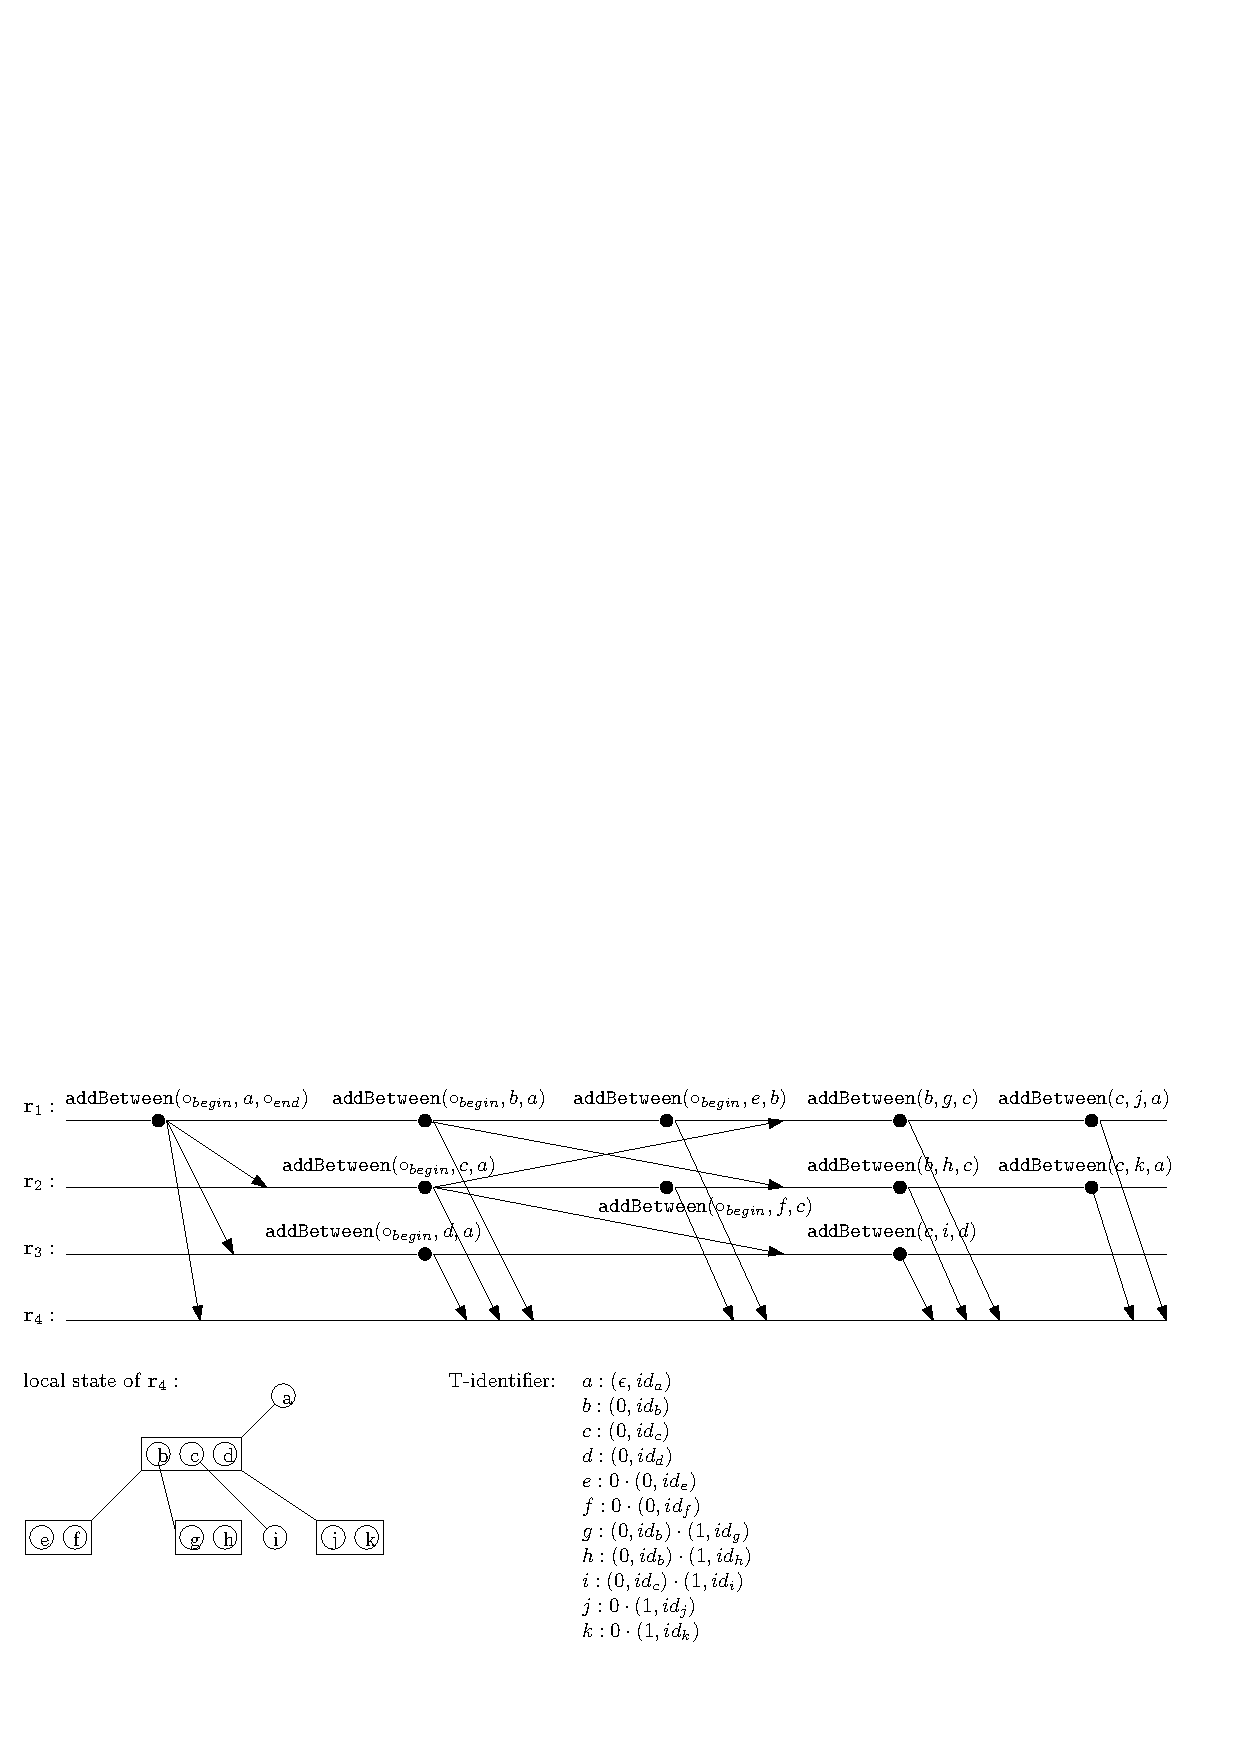
\includegraphics[width=0.85 \textwidth]{figures/TreeDocExecutionandLocalState.pdf}
\vspace{-10pt}
  \caption{An execution of tree-doc, the replica state of replica $\arep_1$ after execution, and the T-identifiers of T-characters.}
  \label{fig:an execution of tree-doc, the local state of replica r1 after execution, and the T-identifiers of T-characters}
\end{figure}


A T-identifier $tid$ of a T-character $w$ is a sequence $tid = c_1 \cdot \ldots \cdot c_n \cdot (p,id)$, where $id$ is a unique identifier, and each for each $1 \leq i \leq n$, $c_i \in \{ 0,1,(1,id')\}$. We call such $id$ the disambiguator of $w$, and require disambiguator to be unique for each T-character. Each $c_i$ of $tid$ represent how to choose the next node in the $i$-th step of the ``path''. If $c_i=0$ (resp., $c_i=1$), then the next node is a node as ``left son'' (resp., ``right son'') of the current (major) node; Else, $c_i = (1,id')$, and this represents that the next node is chosen from ``right sons'' of a minor node with identifier $id'$. The path to the root is fixed to be $\epsilon$.

For example, in \autoref{fig:an execution of tree-doc, the local state of replica r1 after execution, and the T-identifiers of T-characters}, the T-identifier of $w_f$ is $0 \cdot (0,id_f)$, which represent that $w_f$ is a ``left son'' of the root's ``left son'' (could be a major node); the T-identifier of $w_g$ is $(0,id_b) \cdot (1,id_g)$, which represent that $w_g$ is a ``right son'' of minor node $w_b$. Note that, as shown in \autoref{fig:an execution of tree-doc, the local state of replica r1 after execution, and the T-identifiers of T-characters}, the corresponding tree of T-characters is not a binary tree.

We say a set $T$ of T-characters is a T-tree, if:

\begin{itemize}
\setlength{\itemsep}{0.5pt}
\item[-] There exists a T-character of $T$ with T-identifier $(\epsilon,\_)$.

\item[-] Each ghost value of T-character is unique, and each T-character has a unique disambiguator.

\item[-] For each T-character $w=(\_,tid,\_) \in T$, assume $tid = c_1 \cdot \ldots \cdot c_n \cdot (p,id)$. We require that, for each $1 \leq i \leq n$,

    \begin{itemize}
    \setlength{\itemsep}{0.5pt}
    \item[-] If $c_i \in \{ 0,1 \}$, then there exists a T-character $w' = (\_, c_1 \cdot \ldots \cdot c_{i-1} \cdot (c_i,\_) ) \in T$,

    \item[-] Else, if $c_i = (p_i,id_i)$, then there exists a T-character $w' = (\_, c_1 \cdot \ldots \cdot c_{i-1} \cdot (p_i,id_i) ) \in T$, and there exists another T-character $w'' = (\_, c_1 \cdot \ldots \cdot c_{i-1} \cdot (p_i,id'_i) ) \in T$ and $id_i < id'_i$. Or we can say, $w'$ and $w''$ is contained in a same major node, and the disambiguator of $w'$ is less that that of $w''$.
    \end{itemize}
\end{itemize}

Given a T-tree, the order $<_t$, called T-identifier order of this T-tree, is defined as follows: $tid_1 <_t tid_2$, if one of the following cases holds

\begin{itemize}
\setlength{\itemsep}{0.5pt}
\item[-] If $tid_1 = c_1 \cdot \ldots \cdot c_n \cdot (p,id)$, $(tid_2 = c_1 \cdot \ldots \cdot c_n \cdot p \cdot x \cdot l) \vee (tid_2 = c_1 \cdot \ldots \cdot c_n \cdot (p,id) \cdot x \cdot l)$, and $x=1 \vee x=(1,\_)$.

\item[-] If $tid_2 = c_1 \cdot \ldots \cdot c_n \cdot (p,id)$, $tid_1 = c_1 \cdot \ldots \cdot c_n \cdot p \cdot x \cdot l$, and $x=0 \vee x=(0,\_)$.

\item[-] If $tid_1 = c_1 \cdot \ldots \cdot c_n \cdot x_1 \cdot x_2 \cdot l_1$, $tid_2 = c_1 \cdot \ldots \cdot c_n \cdot y_1 \cdot y_2 \cdot l_2$, and one of the following cases holds for some $p \in \{ 0,1 \}$ and $id,id'$:

    \begin{itemize}
    \setlength{\itemsep}{0.5pt}
    \item[-] $x_1=p$, $x_2 \in \{ 0, (0,\_) \}$, and $y_1=(p,\_) \vee (y_1=p \wedge y_2 \in \{ 1, (1,\_) \} )$,

    \item[-] $x_1=(p,id)$, $x_2 \cdot l_1 = \epsilon$, %$y_1=(p,id')$, and $id<id'$,
        and $y_1 = (p,id') \wedge id<id'$,

    \item[-] $x_1=(p,id)$, $x_2 \neq \epsilon$, and $(y_1 = (p,id') \wedge id<id') \vee (y_1=p \wedge y_2 \in \{ 1, (1,\_) \})$.
    \end{itemize}
\end{itemize}

The major node's left descendant is before any minor node and its descendant in $<_t$; minor node are ordered by disambiguator in $<_t$; given minor node $n_a,n_b$ of a same major node, such that the disambiguator of $n_a$ is less than that of $n_b$, then $n_a$ and descendant of $n_a$ is before $n_b$ and descendant of $n_b$ in $<_t$; $n_a$ and descendant of $n_a$ is before the major node's right descendant in $<_t$. We say T-identifier $tid_1$ is a descendant of T-identifier $tid_2$, if $tid_2 = c_1 \cdot \ldots \cdot c_n \cdot (p,id)$, and $tid_1 = c_1 \cdot \ldots \cdot c_n \cdot p \cdot l \vee tid_1 = c_1 \cdot \ldots \cdot c_n \cdot (p,id) \cdot l$.

We define the following function for a set $tree$ of T-charcaters:

\begin{itemize}
\setlength{\itemsep}{0.5pt}
\item[-] $contains(tree,a)$ returns true if there exists a T-character $(a,\_,a)$ in $tree$.

%\item[-] $notAdded(tree,a)$ returns true, if there is no T-character $(\_,\_,a)$ in $tree$. Or we can say, if $a$ has not been added in $tree$.

\item[-] $getTchar(tree,a)$ returns the T-character whose value is $a$ in $tree$.

\item[-] $removeTChar(tree,tid)$ will find the T-character with T-identifier $tid$ in $tree$, and then set the value of this T-character into $nil$.

\item[-] $values(tree)$ returns a sequence, which is obtained by walking the tree according to $<_t$ orders and consider only values of T-characters whose value are not $nil$.
\end{itemize}





\begin{figure}[!h]% {1.0\linewidth}
\begin{lstlisting}[frame=top,caption={Pseudo-code of Tree-Doc algorithm},
captionpos=b,label={lst:Tree-Doc algorithm}]
  payload Set @|$tree$|@
  initial @|$tree$|@ = @|$\emptyset$|@
  initial lin = @|$\epsilon$|@

  addBetween(a,b,c) :
    atSource :
      precondition :  @|$contains(tree,a) \wedge contains(tree,c)$|@, @|$tid_a <_t tid_c$|@, where @|$tid_a$|@ and @|$tid_c$|@ are the T-identifiers of T-characters with value a and c in @|$tree$|@, respectively.
      let @|$tid$|@ be a T-identifier of a T-character in @|$tree$|@, such that, @|$tid_a <_t tid \leq_t tid_c$|@, @|$ \neg \exists (\_,tid',\_) \in tree, tid_a <_t tid' <_t tid$|@
      let id = getTimestamp()
      let @|$w_b$|@ = @|$(b,newID(tid_a,tid,id),b)$|@
      //@ lin = lin@|$\,\cdot\,$|@addBetween(a,b,c)
    downStream(@|$w_b$|@) :
      @|$tree$|@ = @|$tree \cup \{ w_b \}$|@

  remove(a) :
    atSource :
      precondition : @|$contains(tree,a)$|@
      assume @|$getTchar(tree,a) = (a,tid,a)$|@
      //@ lin = lin@|$\,\cdot\,$|@remove(a)
    downStream(tid) :
      @|$removeTChar(tree,tid)$|@

  read() :
    let s = @|$values(string_s)$|@
    //@ lin = lin@|$\,\cdot\,$|@(read()@|$\Rightarrow$|@s)
    return s

  newID(@|$tid_1,tid_2,id$|@)
      precondition : @|$tid_1 <_t tid_2$|@, and @|$\neg \exists (\_,tid,\_) \in tree, tid_1 <_t tid <_t tid_2$|@
    if @|$tid_2$|@ is a descendant of @|$tid_1$|@
      assume @|$tid_2 = l_2 \cdot (p,id_2)$|@
      return @|$l_2 \cdot p \cdot (0,id)$|@
    else if @|$tid_1$|@ is a descendant of @|$tid_2$|@
      assume @|$tid_1 = l_1 \cdot (p,id_1)$|@
      return @|$l_1 \cdot p \cdot (1,id)$|@
    else if @|$tid_1 = l\cdot (p,id_1)$|@, @|$tid_2 = l\cdot (p,id_2)$|@, and @|$id_1 < id_2$|@
      return @|$l \cdot (p,id_1) \cdot (1,id)$|@
    else
      assume @|$tid_1 = l_1 \cdot (p,id_1)$|@
      return @|$l_1 \cdot p \cdot (1,id)$|@
\end{lstlisting}
\end{figure}
% \end{minipage}

$\\$ $\\$

The payload of each replica is a set $tree$ of T-characters. Later we will prove that each replica state $tree$ of replicas during the execution is a T-tree.

To do $\alabelshort[{\tt addBetween}]{a,b,c}$, we first ensure $tree$ contains T-characters of $a$ and $c$, $tid_a <_t tid_c$, where $tid_a$ and $tid_c$ are the T-identifiers of T-characters with value a and c in $tree$, respectively. Then, we find a T-identifier $tid$ of some T-character of $tree$, such that $tid_a <_t tid \leq_t tid_c$, and $tid_a$ and $tid$ are adjacent w.r.t $<_t$. Then, we calls method $newID(tid_a,tid,id)$ to generate a new T-identifier that is with disambiguator $id$ and its T-identifier is between $tid_a$ and $tid$ w.r.t $<_t$, and use this T-identifier to generate a new T-character $w_b$, and put $w_b$ into $tree$.

$newID(tid_1,tid_2,id)$ require that $tid_1$ and $tid_2$ are adjacent w.r.t $<_t$, and it will generate a T-identifier $tid'$, such that $tid_1 <_t tid' <_t tid_2$.

To do $\alabelshort[{\tt remove}]{a}$, we first find the T-identifier $tid$ of T-character with value $a$ in $tree$, and then set the value of T-character with T-identifier $tid$ to be $nil$. To do ${\tt read}$, we return $values(tree)$.




\subsection{Proof of Tree-Doc}
\label{subsec:proof of tree-doc}

As shown in \autoref{fig:an execution of tree-doc, the local state of replica r1 after execution, and the T-identifiers of T-characters}, given a T-tree $tree$, we can draw a tree called major-node-tree of $tree$ as follows: This tree contains tuples $(N,parent)$, such that

\begin{itemize}
\setlength{\itemsep}{0.5pt}
\item[-] $N$ represents set of nodes. Each element in $Node$ is a list $w_1 \cdot \ldots \cdot w_n$ of a major node $\{ w_1,\ldots,w_n \}$ of $tree$, while $w_1,\ldots,w_n$ are ordered by their disambiguators.

\item[-] $parent \in N \times N$ represents the parent relation. $(node_1,node_2) \in parent$, if the T-identifiers of T-characters of $node_1$ is of the form $c_1 \cdot \ldots \cdot c_n \cdot (p,\_)$, one of the following cases holds:

    \begin{itemize}
    \setlength{\itemsep}{0.5pt}
    \item[-] The T-identifiers of T-characters of $node_2$ is of the form $c_1 \cdot \ldots \cdot c_n \cdot p \cdot (p',\_)$. If $p'=0$, we say that $node_2$ is a ``left son'' of $node_1$; else, if $p'=1$, we say that $node_2$ is a ``right son'' of $node_1$.

    \item[-] The T-identifiers of T-characters of $node_2$ is of the form $c_1 \cdot \ldots \cdot c_n \cdot (p,id_p) \cdot (p',\_)$, while $c_1 \cdot \ldots \cdot c_n \cdot (p,id_p)$ is a T-identifier of T-characters $w_1$ of $node_1$. We say that $node2$ is a ``right son'' of $w_1$.

    \item[-] There exists $node_0 \in N$, such that the T-identifier of T-characters of $node_0$ is $\epsilon$.
    \end{itemize}
\end{itemize}

According to the definition of T-tree, in the major-node-tree $(N,parent)$ of $tree$, it is easy to see that,

\begin{itemize}
\setlength{\itemsep}{0.5pt}
\item[-] For each $node_2 \in N$, if the T-identifier of T-characters of $node_2$ is not $\epsilon$, then, there exists only one $node_1 \in N$, such that $(node_1,node_2) \in parent$. Or we can say, for each node, if it is not the root, then it has only one parent.

\item[-] Given $node_2 \in N$, if the T-identifier of T-characters of $node_2$ is $\epsilon$, then, there does not exist $node_1 \in N$, such that $(node_1,node_2) \in parent$. Or we can say, the root node has no parent.

\item[-] The relation $parent$ is acyclic.
\end{itemize}

The following lemma state that, the T-identifier order $<_t$ of a T-tree is a total and acyclic order.

\begin{lemma}
\label{lemma:the <t order is a total and acyclic order}
Given a T-tree $tree$ and the T-identifier order $<_t$ of $tree$, then, $<_t$ is a total and acyclic order.
\end{lemma}

\begin {proof}
Let us prove that $<_t$ is a total order. Given T-identifiers $tid_1 = c_1 \cdot \ldots \cdot c_n \cdot (p,id)$ and $tid_2 = c'_1 \cdot \ldots \cdot c'_m \cdot (p',id')$.

\begin{itemize}
\setlength{\itemsep}{0.5pt}
\item[-] If $tid_1$ is a descendant of $tid_2$, then we have $tid_1 <_t tid_2 \vee tid_2 <_t tid_1$. Similarly, if $tid_2$ is a descendant of $tid_1$, then we have $tid_1 <_t tid_2 \vee tid_2 <_t tid_1$.

\item[-] If $tid_1$ is not a descendant of $tid_1$ and $tid_1$ is not a descendant of $tid_2$. We can see that there exists $c''_1,\ldots,c''_k$, such that $tid_1 = c''_1 \cdot \ldots \cdot c''_k \cdot x_1 \cdot x_2 \cdot l_1$, $tid_2 = c''_1 \cdot \ldots \cdot c''_k \cdot y_1 \cdot y_2 \cdot l_2$, and $x_1 \neq y_1$. Then,

    \begin{itemize}
    \setlength{\itemsep}{0.5pt}
    \item[-] If $x_1 \in \{ 0, (0,\_) \}$ and $y_1 \in \{ 1, (1,\_) \}$, then $tid_1 <_t tid_2$.

    \item[-] Else, if $x_1=p_u$ and $y_1 = (p_u,id_u)$ for some $p_u \in \{ 0,1 \}$. Since $tid_1$ is not a descendant of $tid_1$ and $tid_1$ is not a descendant of $tid_2$, we can see that $x_2 \neq \epsilon \wedge y_2 \neq \epsilon$. Then,

        \begin{itemize}
        \setlength{\itemsep}{0.5pt}
        \item[-] If $x_2 \in \{ 0, (0,\_) \}$, we have $tid_1 <_t tid_2$,
        \item[-] Else, if $x_2 \in \{ 1, (1,\_) \}$, we have $tid_2 <_t tid_1$.
        \end{itemize}

    \item[-] Else, $x_1 = (p_u,id_u)$, $y_1 = (p_u,id'_u)$, $p \in \{0,1 \}$ and $id_u \neq id'_u$. Then,

        \begin{itemize}
        \setlength{\itemsep}{0.5pt}
        \item[-] If $id_u < id'_u$, we have $tid_1 <_t tid_2$,
        \item[-] Else, if $id'_u < id_u$, we have $tid_2 <_t tid_1$.
        \end{itemize}
    \end{itemize}
\end{itemize}

Therefore, $<_t$ is a total order.

Let us prove that $<_t$ is acyclic. Given the major-node-tree $(M,parent)$ of $tree$ and an element $node \in N$, assume $node = w_1 \cdot \ldots \cdot w_n$. Assume for each $i$, $w_i = (v_i,tid_i,gv_i)$. Then, it is easy to see that,

\begin{itemize}
\setlength{\itemsep}{0.5pt}
\item[-] $w^l <_t w^r$, where $w^l$ is a W-character belongs to a node that is (a descendant of) the ``left son'' of $node$, and $w^r$ is a W-character belongs to a node that is (a descendant of) the ``right son'' of $node$.

\item[-] $w^l <_t w^i$, where $w^l$ is a W-character belongs to a node that is (a descendant of) the ``left son'' of $node$, and $w^i$ is either $w_i$, or a W-character belongs to a node that is a ``descendent'' of $w_i$.

\item[-] Given $i<j$, we have $w^i <_t w^j$, where $w^i$ (resp., $w^j$) is either $w_i$ (resp., $w_j$), or a W-character belongs to a node that is a ``descendent'' of $w_i$ (a ``descendent'' of $w_j$).

\item[-] $w^i <_t w^r$, where $w^i$ is either $w_i$, or a W-character belongs to a node that is a ``descendent'' of $w_i$, and $w^r$ is a W-character belongs to a node that is (a descendant of) the ``right son'' of $node$.
\end{itemize}

Therefore, we can see that $<_t$ is a order for traversing the W-characters of the major-node-tree. For each node $node = w_1 \cdot \ldots \cdot w_n \in N$, we first traverse W-characters in its ``left son'' of $node$ and the descendant of this ``left son''; then, for each $i$, we traverse $w_i$ and W-characters in nodes of descendant of $w_i$; finally, we traverse W-characters in its ``right son'' of $node$ and the descendant of this ``right son''. This process never goes back. Therefore, it is easy to see that $<_t$ is acyclic. This completes the proof of this lemma. $\qed$
\end {proof}


The following lemma state that, if we add a T-character (an effector) into a T-tree, then, we obtain another T-tree.

\begin{lemma}
\label{lemma:if we add a T-character (an effector) into a T-tree, then we obtain another T-tree}
Given an effector $w_b = (b,tid_b,b)$ of an operation $\alabel = \alabelshort[{\tt addBetween}]{a,b,c}$, assume $\alabel$ calls $\alabelshort[{\tt newID}]{tid_a,tid,id}$ to generate effector $w_b$. Given a T-tree $tree$, assume that $(\_,tid_a,a),(\_,tid,\_) \in tree$, no T-character of $tree$ has ghost value $b$, no T-character of $tree$ has disambiguator $id$. Then, $tree \cup \{ w_b \}$ is a T-tree.
\end{lemma}

\begin {proof}
Assume that $tid_a = c_1 \cdot \ldots \cdot c_n \cdot (p_a,id_a)$, $tid = c'_1 \cdot \ldots \cdot c'_m \cdot (p',id')$. Then, according to the method {\tt newID}, we can see that $tid_b \in \{ c'_1 \cdot \ldots \cdot c'_m \cdot p' \cdot (0,id), c_1 \cdot \ldots \cdot c_n \cdot p_a \cdot (1,id), c_1 \cdot \ldots \cdot c_n \cdot (p_a,id_a) \cdot (1,id) \}$. When $tid_b = c_1 \cdot \ldots \cdot c_n \cdot (p_a,id_a) \cdot (1,id)$, according to method {\tt neweID}, we can see that $tid_a = c_1 \cdot \ldots \cdot c_n \cdot (p_a,id_a)$, $tid = c_1 \cdot \ldots \cdot c_n \cdot (p_a,id')$, and $id_a < id'$. Since $tree$ is already a T-tree, no T-character of $tree$ has ghost value $b$, no T-character of $tree$ has disambiguator $id$, then, for each possible value of $tid_b$, it is easy to see that $tree \cup \{ w_b \}$ is a T-tree. $\qed$
\end {proof}

The following lemma state that, when we do $\alabelshort[{\tt addBetween}]{a,b,c}$ and generate an effector $(b,tid_b,b)$, then $tid_b$ is between T-identifiers of T-characters of $a$ and $c$.

\begin{lemma}
\label{lemma:when we do addBetween(a,b,c) and generate an effector (b,tid_b,b) with newID(tid_a,tid_x,id), then tid_b is between tid_a and tid_x}
Assume the current replica state is a T-tree $tree$, we do an operation $\alabel = {\tt addBetween}($ $a,b,c)$ and generate an effector $w_b = (b,tid_b,b)$, and this process calls $\alabelshort[{\tt newID}]{tid_a,tid,id}$. Let $<_t$ be the T-identifier order of the T-tree $tree \cup \{ w_b \}$. Then, we have that, $tid_a <_t tid_b <_t tid$.
\end{lemma}

\begin {proof}
Since we assume each value is put only once, and $\alabelshort[{\tt getTimestamp}]{}$ always return a unique disambiguator, by Lemma \ref{lemma:if we add a T-character (an effector) into a T-tree, then we obtain another T-tree}, we can see that $tree \cup \{ w_b \}$ is a T-tree.

By the tree-doc algorithm, it is obvious that $(a,tid_a,a),(c,\_,c) \in tree$, $tid$ is a T-identifier of a T-character in $tree$, $tid_a <_t tid \leq_t tid_c$, $ \neg \exists (\_,tid',\_) \in tree$, such that $tid_a <_t tid' <_t tid$.

Let us consider all possible cases of $tid_a$ and $tid$, and shows that $tid_a <_t tid'' <_t tid$, where $tid''$ is the return value of $\alabelshort[{\tt newID}]{tid_a,tid,id}$.

\begin{itemize}
\setlength{\itemsep}{0.5pt}
\item[-] If $tid$ is a descendant of $tid_a$: Then, $tid$ is either a ``right son'' of $tid_a$, or a descendant of a ``right son'' of $tid_a$ (or its minor node). We can see that $tid_2$ does not have ``left son''.

    Assume that $tid = l_2 \cdot (p_2,id_2)$, then, $tid'' = l_2 \cdot p_2 \cdot (0,id)$. We can see that $tid''$ is a ``son'' of ``right son'' of $tid_a$, or a ``son'' of a descendant of ``right son'' of $tid_a$ (or its minor node), and thus, $tid_a <_t tid''$. Since $tid''$ is a ``left son'' of $tid$, we can see that $tid'' <_t tid$.

\item[-] If $tid_a$ is a descendant of $tid$: Then, $tid_a$ is either a ``left son'' of $tid$, or a descendant of a ``left son'' of $tid$ (or its minor node). We can see that $tid_a$ does not have ``right son''.

    Assume that $tid_a = l_1 \cdot (p_1,id_1)$, then, $tid'' = l_1 \cdot p_1 \cdot (1,id)$. We can see that $tid''$ is a ``son'' of ``left son'' of $tid$, or a ``son'' of a descendant of ``left son'' of $tid$ (or its minor node), and thus, $tid'' <_t tid$. Since $tid''$ is a ``right son'' of $tid_a$, we can see that $tid_a <_t tid''$.

\item[-] Otherwise, there are two possibilities:
    \begin{itemize}
    \setlength{\itemsep}{0.5pt}
    \item[-] If $tid_a = l \cdot (p,id_1)$, $tid = l \cdot (p,id_2)$, and $id_1 < id_2$: We can see that $tid_a$ does not have ``right son''.

    Let $tid'' = l \cdot (p,id_1) \cdot (1,id)$. Since $tid''$ is a ``right son'' of $tid_a$, we can see that $tid_a <_t tid''$. Since $id_1 < id_2$, we can see that $tid'' <_t tid$.

    \item[-] There exists $tid_0$, such that $tid_0 = l \cdot (p,id_0)$, $tid = l \cdot (p,id_2)$, $id_0 < id_2$, and $tid_a$ is a descendant of $tid_0$: We can see that $tid_a$ does not have ``right son''.

    Assume that $tid_a = l \cdot (p,id_0) \cdot l_2 \cdot (p',id'_1)$, then, $tid'' = l \cdot (p,id_0) \cdot l_2 \cdot p' \cdot (1,id)$. We can see that $tid''$ is a ``right son'' of $tid_a$, and thus, $tid_a <_t tid''$. Since $id_0 < id_2$, we can see that $tid'' <_t tid$.
    \end{itemize}

\end{itemize}

This completes the proof of this lemma. $\qed$
\end {proof}


Then, let us prove that tree-doc is \crdtlinearizable{} w.r.t $\specWooki$.

\begin{lemma}
\label{lemma:tree-doc is correct}
Tree-doc is \crdtlinearizable{} w.r.t $\specWooki$.
\end{lemma}

\begin {proof}

Let us first prove that, during the executions, each replica state is a T-tree. Recall that each value is put only once, and $\alabelshort[{\tt getTimestamp}]{}$ always return a unique disambiguator.

\begin{itemize}
\setlength{\itemsep}{0.5pt}
\item[-] The initial replica state for each replica is obviously a T-tree.

\item[-] When a replica do generator of an operation $\alabel = \alabelshort[{\tt addBetween}]{a,b,c}$ and then apply its effector: Assume the original replica state is $\sigma$, the effector of $\alabel$ is $(b,tid_b,b)$, and we call $\alabelshort[{\tt newID}]{tid_a,tid,id}$ to generate $tid_b$. By tree-doc algorithm, it is obvious that, $(,tid_a,a),(\_,$ $tid,\_) \in \sigma$. It is obvious that after we apply the effector, the replica state is $\sigma \cup \{ (b,tid_b,b) \}$. Then, by Lemma \ref{lemma:if we add a T-character (an effector) into a T-tree, then we obtain another T-tree}, we can see that $\sigma \cup \{ (b,tid_b,b) \}$ is a T-tree.

\item[-] When a replica $\arep$ apply effector that corresponds to an operation $\alabel = \alabelshort[{\tt addBetween}]{a,b,c}$ originated in a different replica: Assume the original replica state of replica $\arep$ is $\sigma$, the effector of $\alabel$ is $(b,tid_b,b)$. Assume $\alabel$ is done in replica $\arep'$, and we call $\alabelshort[{\tt newID}]{tid_a,tid,id}$ to generate $tid_b$. By tree-doc algorithm, it is obvious that, $(,tid_a,a),(\_,$ $tid,\_)$ is in the replica state of $\arep'$ when $(b,tid_b,b)$ is applied in replica $\arep'$. By the causal delivery assumption, we can see that $(\_,tid_a,a),(\_,$ $tid,\_)$ is in the replica state of replica $\arep$ before $(b,tid_b,b)$ is applied. It is obvious that after we apply the effector in replica $\arep$, the replica state is $\sigma \cup \{ (b,tid_b,b) \}$. Then, by Lemma \ref{lemma:if we add a T-character (an effector) into a T-tree, then we obtain another T-tree}, we can see that $\sigma \cup \{ (b,tid_b,b) \}$ is a T-tree.
\end{itemize}

Therefore, during the executions, each replica state is a T-tree.

A refinement mapping $\refmap$ is given as follows: Given a replica state $\sigma$ that is a T-tree. Assume that $\sigma = \{ w_1,\ldots,w_n\}$, and for each $i$, $w_i = (v_i,tid_i,gv_i)$. Then, the refinement mapping $\refmap(\sigma) = (l,T)$, where $l$ is obtained by walking $\sigma$ and read ghost value of each T-characters according to the T-identifier order $<_t$ of $\sigma$, and $T = \{ gv_i \vert v_i = nil \}$. By Lemma \ref{lemma:the <t order is a total and acyclic order}, we know that $<_t$ is a total and acyclic order. Therefore, our construction of $\refmap$ has definition.

Our proof proceeds as follows:

\begin{itemize}
\setlength{\itemsep}{0.5pt}
\item[-] Since the effector of {\tt addBetween} do set union, we can see that the effectors of concurrent {\tt addBetween} operations commute. According to tree-doc algorithm, it is easy to see that the effector of concurrent {\tt remove} operations commute, since they both set the value of some T-characters into $nil$. Concurrent {\tt addBetween} and a {\tt remove} effectors commute, since the T-character changed by {\tt remove} are different from the T-character added by the {\tt addBetween}.

    Let us prove $\mathsf{ReplicaStates}$: Since every operation is appended to the linearization when it executes atSource it clearly follows, the linearization order is consistent with visibility order. Then, by the causal delivery assumption, the order in which effectors are applied at a given replica is also consistent with the visibility order. Let $\alinord_1$ be the projection of linearization order into labels of effectors applied in a replica $\arep$, and $\alinord_2$ be the order of labels of effectors applied in replica $\arep$. By Lemma \ref{lemma:given two sequence consistent with visibility order, one can be obtained from the other}, $\alinord_2$ can be obtained from $\alinord_1$ by several time of swapping adjacent pair of concurrent operations. We have already proved that effector of concurrent operations commute. Therefore, we know that $\mathsf{ReplicaStates}$ is an inductive invariant.

    Note that, by the causal delivery assumption and tree-doc algorithm, it cannot happen that an $\alabelshort[{\tt addBetween}]{a,b,c}$ operation adding ${\tt b}$ between ${\tt a}$ and ${\tt c}$ is concurrent with an operation that adds ${\tt a}$ or ${\tt c}$ or ${\tt x}$ to the list, where the T-identifier of T-character of $x$ is $tid_x$ and we use $\alabelshort[{\tt newID}]{tid_a,tid_x,id}$ to generate the effector of $\alabelshort[{\tt addBetween}]{a,b,c}$. It cannot happen that an $\alabelshort[{\tt addBetween}]{a,b,c}$ operation adding ${\tt b}$ is concurrent with an operation $\alabelshort[{\tt remove}]{b}$ that removes ${\tt b}$. This ensures that reordering concurrent effectors doesn't lead to ``invalid'' replica states such as the replica state does not contains T-character of $a$ or $c$ or $x$ while the effector requires to put $b$ between $a$ and $c$ and use $\alabelshort[{\tt newID}]{tid_a,tid_x,id}$ to generate the effector of $\alabelshort[{\tt addBetween}]{a,b,c}$ (which would happen if $\alabelshort[{\tt addBetween}]{\_,a,\_}$ or $\alabelshort[{\tt addBetween}]{\_,c,\_}$ or $\alabelshort[{\tt addBetween}]{\_,x,\_}$ is delivered before $\alabelshort[{\tt addBetween}]{a,b,c}$), or a replica state does not contain T-character of $b$ when effector requires to remove $b$ (which would happen if $\alabelshort[{\tt remove}]{b}$ is delivered before $\alabelshort[{\tt addAfter}]{\_,b,\_}$).

\item[-] Let us prove $\mathsf{Refinement}$:
    \begin{itemize}
    \setlength{\itemsep}{0.5pt}
    \item[-] Assume $\refmap(\sigma) = (l,T)$. If $\sigma'$ is obtained from $\sigma$ by applying an effector $\delta$ produced by an operation $\alabel = \alabelshort[{\tt addBetween}]{a,b,c}$. Assume the effector is $w_b = (b,tid_b,b)$. Obviously, $\sigma' = \sigma \cup \{ w_b \}$ and $\sigma'$ is also a T-tree. We need to prove that $\refmap(\sigma) \specarrow{\alabelshort[{\tt addBetween}]{a,b,c}} \refmap(\sigma')$.

        Assume in the source replica of $\alabel$, it calls $\alabelshort[{\tt newID}]{tid_a,tid_x,id}$ to generate $tid_b$. Let $tid_c$ be the T-identifier of T-character with value $c$ in the source replica of $\alabel$, and let $<'_t$ be the T-identifier order in the source replica of $\alabel$ when $w_b$ is applied. By Lemma \ref{lemma:when we do addBetween(a,b,c) and generate an effector (b,tid_b,b) with newID(tid_a,tid_x,id), then tid_b is between tid_a and tid_x}, we can see that $tid_a <'_t tid_b <'_t tid_x$. According to tree-doc algorithm, we can see that $tid_a <'_t tid_x <'_t tid_c$.

        It is easy to see that, given T-trees $tree_1$ and $tree_2$, if the T-identifiers of T-characters of $tree_1$ is a subset of that of $tree_2$, then the T-identifier order of $tree_1$ is a subset of that of $tree_2$.

        Let $tree_b$ be the replica state in the source replica of $\alabel$ when $w_b$ is applied. By the causal delivery assumption, we can see that all T-characters (effectors) of $tree_b$ have already been applied in $\sigma'$. Let $<_{t\sigma'}$ be the T-identifier order of $\sigma'$. Then, we can see that, $tid_a <_{t\sigma'} tid_b <_{t\sigma'} tid_x <_{t\sigma'} tid_c$.

        Assume $\refmap(\sigma') = (l',T')$. Then, it is easy to see that $T = T'$, and $l'$ is obtained from $l$ by putting $b$ into some postiion between $a$ and $c$. Therefore, $\refmap(\sigma) \specarrow{\alabelshort[{\tt addBetween}]{a,b,c}} \refmap(\sigma')$.

    \item[-] Assume $\refmap(\sigma) = (l,T)$. If $\sigma'$ is obtained from $\sigma$ by applying an effector $\delta$ produced by an operation $\alabelshort[{\tt remove}]{a}$. By the causal delivery assumption, we can see that a T-character $w_a$ with ghost value $a$ is already in $\sigma$, and then, $a \in l$. By the tree-doc algorithm, we can see that $\sigma'$ is obtained from $\sigma$ by setting the value of $w_a$ into $nil$. Let $\refmap(\sigma) = (l',T')$. It is obvious that $l=l'$, and $T' = T \cup \{ a \}$. Thus, we have $\refmap(\sigma) \specarrow{\alabelshort[{\tt remove}]{a}} \refmap(\sigma')$.

    \item[-] Assume we do $\alabellong[{\tt read}]{}{s}{}$ on replica state $\sigma$. Assume $\sigma = \{w_1,\ldots,w_n\}$, and for each $i$, $w_i = (v_i,tid_i,gv_i)$. Then, $s$ is obtained by walking $\sigma$ and read value of each T-characters according to the T-identifier order $<_t$ of $\sigma$, and ignoring all $nil$. Assume $\refmap(\sigma) = (l,T)$. We can see that $l$ is obtained by walking $\sigma$ and read ghost value of each T-characters according to the T-identifier order $<_t$ of $\sigma$, and $T = \{ gv_i \vert v_i = nil \}$. Thus, we have $\refmap(\sigma) \specarrow{\alabellong[{\tt read}]{}{s}{}} \refmap(\sigma)$.
    \end{itemize}

\item[-] We have already prove that $\mathsf{ReplicaStates}$ is an inductive invariant and $\mathsf{Refinement}$ holds. Then, similarly as in \sectionautorefname \ref{subsec:time order of execution as linearization}, we can prove that $\mathsf{\CRDTLinshort{}}$ is an inductive invariant.
\end{itemize}

This completes the proof of this lemma. $\qed$
\end {proof}











\section{Discussion about List with {\tt addAt} Interface}
\label{sec:discussion about list with addAt interface}



\subsection{A first version of list with {\tt addAt} Interface}
\label{subsec:a first version of list with addAt interface}

The first version of list with {\tt addAt} interface is as follows: A list uses the following three methods:

\begin{itemize}
\setlength{\itemsep}{0.5pt}
\item[-] $\alabelshort[{\tt addAt}]{a,k}$: Inserts value $a$ into position $k$ of the list of replica state. For $k$ exceeding the list size of replica state, $k$ will be inserted at the end of the list.

\item[-] $\alabelshort[{\tt remove}]{a}$: Remove value $a$ from list of the replica state.

\item[-] $\alabellong[{\tt read}]{}{s}{}$: Returns the list content of the replica state.
\end{itemize}

Here we assume the first element of a sequence is at position $0$.

Our RGA algorithm of \sectionautorefname \ref{sec:overview} can be modified as follows for this interface: To do $\alabelshort[{\tt addAt}]{a,k}$, we work as follows:

\begin{itemize}
\setlength{\itemsep}{0.5pt}
\item[-] Let $s = traverse(N, Tomb)$ be the list content in replica state. If $s = \epsilon$, then let $b = \circ$; else, if $\vert s \vert \geq k$, then let $b=s[k-1]$; else, let $b=s[\vert s \vert -1]$.

\item[-] Work as $\alabelshort[{\tt addAfter}]{b,a}$. Especially, the effector of $\alabelshort[{\tt addAt}]{a,k}$ is the effector of ${\tt addAfter}(b,$ $a)$.
\end{itemize}



\subsection{Two Sequential Specification for list with {\tt addAt} Interface}
\label{subsec:two sequential specification for list with addAt interface}

Depending on whether use tombstone or not, there are two sequential specification for list with {\tt addAt} interface.

\noindent {\bf Sequential specification $\specAddatOne$}: The first sequential specification $\specAddatOne$ of list with {\tt addAt} interface does not use tombstone. Each abstract state $\abstate = l$ contains a sequence $l$ of elements of a given type. The element $l$ is the list of values that has been input and not removed yet. The sequential specification $\specAddatOne$ of list with {\tt addAt} interface is given with the transitions as follows:
\[
  \begin{array}{rcl}
    \big(\ l_1 \cdot l_2 \ |\ a\text{ is fresh}\ , \vert l_1 \vert = k \big)
     & \specarrow{\alabelshort[\mathtt{addAt}]{a,k}}
     & l_1 \cdot a \cdot l_2 \\
      \big(\ l \ |\ a\text{ is fresh}\ , \vert l \vert < k \big)
     & \specarrow{\alabelshort[\mathtt{addAt}]{a,k}}
     & l \cdot a \\
     l_1 \cdot a \cdot l_2
     & \specarrow{\alabelshort[\mathtt{remove}]{a}}
     & l_1 \cdot l_2 \\
     l
     & \specarrow{\alabellong[\mathtt{read}]{}{l}{}}
     & l
   \end{array}
\]

If $\vert l_1 \cdot l_2 \vert \geq k$ and $\vert l_1 \vert = k$, Method $\alabelshort[\mathtt{addAt}]{a,k}$ puts $a$ immediately after $l_1$; Else, if $\vert l \vert <k$, Method $\alabelshort[\mathtt{addAt}]{a,k}$ puts $a$ immediately after $l$. Method $\alabelshort[\mathtt{remove}]{a}$ remove $a$ from $l_1 \cdot a \cdot l_2$. $\alabellong[\mathtt{read}]{}{l}{}$ returns the list.


\noindent {\bf Sequential specification $\specAddatTwo$}: The second sequential specification $\specAddatTwo$ of list with {\tt addAt} interface uses tombstone. Each abstract state $\abstate = (l,T)$ contains a sequence $l$ of elements of a given type and a set $T$ of elements appearing in the list. The element $l$ is the list of all input values, whether already removed or not; while $T$ stores the removed values and is used as \emph{tombstone}. The sequential specification $\specAddatTwo$ of list with {\tt addAt} interface is given with the transitions as follows:

\[
  \begin{array}{rcl}
    \big(\ (l_1 \cdot l_2,T\big)\ |\ a\text{ is fresh}\ , \vert l_1 \vert = k \big)
     & \specarrow{\alabelshort[\mathtt{addAt}]{a,k}}
     & (l_1 \cdot a \cdot l_2,T)\\
     \big(\ (l,T\big)\ |\ a\text{ is fresh}\ , \vert l \vert < k \big)
     & \specarrow{\alabelshort[\mathtt{addAt}]{a,k}}
     & (l \cdot a,T)\\
     \big(\ (l,T)\ |\ a\ \text{occurs in}\ l\ \big)
     & \specarrow{\alabelshort[\mathtt{remove}]{a}}
     & (l,T \cup \{a\})\\
     (l,T)
     & \specarrow{\alabellong[\mathtt{read}]{}{s}{}}
     & (l,T)\
       \left[\begin{array}{c}
           \text{with $s$ is obtained from $l$}\\
           \text{by removing the values in $T$}
       \end{array}\right]
   \end{array}
\]

If $\vert l_1 \cdot l_2 \vert \geq k$ and $\vert l_1 \vert = k$, Method $\alabelshort[\mathtt{addAt}]{a,k}$ puts $a$ immediately after $l_1$; Else, if $\vert l \vert <k$, Method $\alabelshort[\mathtt{addAt}]{a,k}$ puts $a$ immediately after $l$. Method $\alabelshort[\mathtt{remove}]{a}$ adds $a$ into $T$, hence removing $a$ from the list for subsequent calls to the $\mathtt{read}$ method. Thus, $\alabellong[\mathtt{read}]{}{s}{}$ returns the list content excluding any element appearing in $T$.



\subsection{RGA not \crdtlinearizable{} w.r.t $\specAddatOne$ or $\specAddatTwo$}
\label{subsec:RGA not RA-linearizable w.r.t specAddatOne or SpecAddatTwo}

\autoref{fig:an example history shows that RGA is not RA-linearizable w.r.t specAddat} shows an example that is a history of RGA and is not \crdtlinearizable{} w.r.t $\specAddatOne$ or $\specAddatTwo$. Here we assume that $\ats_a < \ats_b < \ats_c < \ats_d < \ats_e$. We also draw the replica state of replica $r_2$ and $r_3$ after the execution of $h$ in \autoref{fig:an example history shows that RGA is not RA-linearizable w.r.t specAddat}.


\begin{figure}[!h]
  \centering
  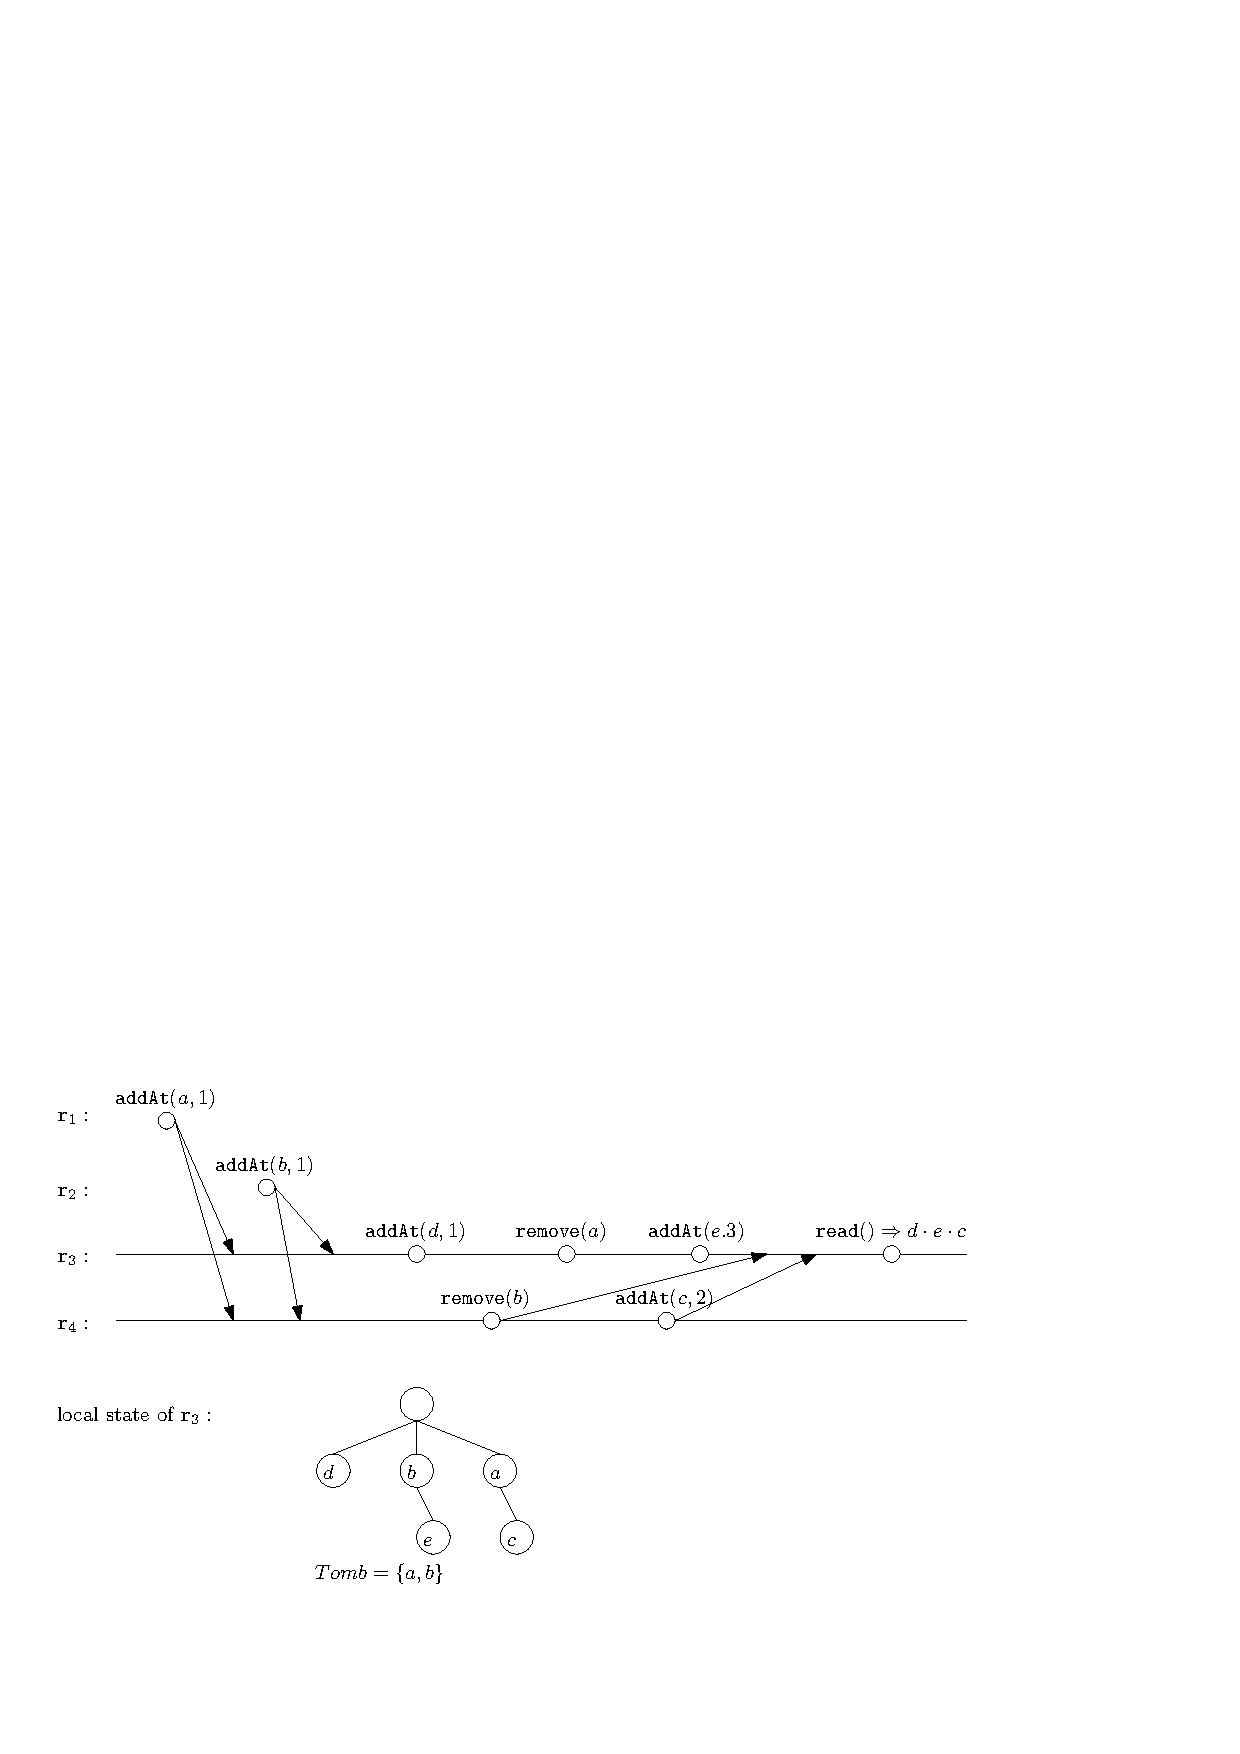
\includegraphics[width=0.9 \textwidth]{figures/RGAwithaddAtNotRALin.pdf}
\vspace{-10pt}
  \caption{An example history shows that RGA is not \crdtlinearizable{} w.r.t .}
  \label{fig:an example history shows that RGA is not RA-linearizable w.r.t specAddat}
\end{figure}

The following lemma states that RGA is not \crdtlinearizable{} w.r.t $\specAddatOne$ or $\specAddatTwo$.

\begin{lemma}
\label{lemma:The history h of fig an example history shows that RGA is not RA-linarizable w.r.t specAddat is not RA-linearizable w.r.t SpecAddatOne or SpecAddatTwo}
RGA is not \crdtlinearizable{} w.r.t $\specAddatOne$ or $\specAddatTwo$.
\end{lemma}

\begin {proof}
Let $h$ be the history of \autoref{fig:an example history shows that RGA is not RA-linearizable w.r.t specAddat}. Let $h'$ be obtained from $h$ by removing the $\alabellong[\mathtt{read}]{}{a \cdot c}{}$ operation of replica $r_2$. It is obvious that $h'$ is also a history of RGA.

We prove that RGA is not \crdtlinearizable{} w.r.t $\specAddatOne$ by proving that $h'$ is not \crdtlinearizable{} w.r.t $\specAddatOne$, and we prove this by showing that all possible linarizations of $h'$ are not admitted by the sequential specification.

\begin{itemize}
\setlength{\itemsep}{0.5pt}
\item[-] $\epsilon \specarrow{\alabelshort[\mathtt{addAt}]{a,0}}$ $a \specarrow{\alabelshort[\mathtt{addAt}]{b,0}}$ $b \cdot a \specarrow{\alabelshort[\mathtt{remove}]{b}}$ $a \specarrow{\alabelshort[\mathtt{addAt}]{c,1}}$ $a \cdot c \specarrow{\alabelshort[\mathtt{addAt}]{d,0}}$ $d \cdot a \cdot c \specarrow{\alabelshort[\mathtt{remove}]{a}}$ $d \cdot c \specarrow{\alabelshort[\mathtt{addAt}]{e,2}}$ $d \cdot c \cdot e \specarrow{\alabellong[\mathtt{read}]{}{d \cdot c \cdot e}{}} d \cdot c \cdot e$.

\item[-] $\epsilon \specarrow{\alabelshort[\mathtt{addAt}]{a,0}}$ $a \specarrow{\alabelshort[\mathtt{addAt}]{b,0}}$ $b \cdot a \specarrow{\alabelshort[\mathtt{remove}]{b}}$ $a \specarrow{\alabelshort[\mathtt{addAt}]{d,0}}$ $d \cdot a \specarrow{\alabelshort[\mathtt{addAt}]{c,1}}$ $d \cdot c \cdot a \specarrow{\alabelshort[\mathtt{remove}]{a}}$ $d \cdot c \specarrow{\alabelshort[\mathtt{addAt}]{e,2}}$ $d \cdot c \cdot e \specarrow{\alabellong[\mathtt{read}]{}{d \cdot c \cdot e}{}} d \cdot c \cdot e$.

\item[-] $\epsilon \specarrow{\alabelshort[\mathtt{addAt}]{a,0}}$ $a \specarrow{\alabelshort[\mathtt{addAt}]{b,0}}$ $b \cdot a \specarrow{\alabelshort[\mathtt{remove}]{b}}$ $a \specarrow{\alabelshort[\mathtt{addAt}]{d,0}}$ $d \cdot a \specarrow{\alabelshort[\mathtt{remove}]{a}}$ $d \specarrow{\alabelshort[\mathtt{addAt}]{c,1}}$ $d \cdot c \specarrow{\alabelshort[\mathtt{addAt}]{e,2}}$ $d \cdot c \cdot e \specarrow{\alabellong[\mathtt{read}]{}{d \cdot c \cdot e}{}} d \cdot c \cdot e$.

\item[-] $\epsilon \specarrow{\alabelshort[\mathtt{addAt}]{a,0}}$ $a \specarrow{\alabelshort[\mathtt{addAt}]{b,0}}$ $b \cdot a \specarrow{\alabelshort[\mathtt{remove}]{b}}$ $a \specarrow{\alabelshort[\mathtt{addAt}]{d,0}}$ $d \cdot a \specarrow{\alabelshort[\mathtt{remove}]{a}}$ $d \specarrow{\alabelshort[\mathtt{addAt}]{e,2}}$ $d \cdot e \specarrow{\alabelshort[\mathtt{addAt}]{c,1}}$ $d \cdot c \cdot e \specarrow{\alabellong[\mathtt{read}]{}{d \cdot c \cdot e}{}} d \cdot c \cdot e$.

\item[-] $\epsilon \specarrow{\alabelshort[\mathtt{addAt}]{a,0}}$ $a \specarrow{\alabelshort[\mathtt{addAt}]{b,0}}$ $b \cdot a \specarrow{\alabelshort[\mathtt{addAt}]{d,0}}$ $d \cdot b \cdot a \specarrow{\alabelshort[\mathtt{remove}]{b}}$ $d \cdot a \specarrow{\alabelshort[\mathtt{addAt}]{c,1}}$ $d \cdot c \cdot a \specarrow{\alabelshort[\mathtt{remove}]{a}}$ $d \cdot c \specarrow{\alabelshort[\mathtt{addAt}]{e,2}}$ $d \cdot c \cdot e \specarrow{\alabellong[\mathtt{read}]{}{d \cdot c \cdot e}{}} d \cdot c \cdot e$.

\item[-] $\epsilon \specarrow{\alabelshort[\mathtt{addAt}]{a,0}}$ $a \specarrow{\alabelshort[\mathtt{addAt}]{b,0}}$ $b \cdot a \specarrow{\alabelshort[\mathtt{addAt}]{d,0}}$ $d \cdot b \cdot a \specarrow{\alabelshort[\mathtt{remove}]{b}}$ $d \cdot a \specarrow{\alabelshort[\mathtt{remove}]{a}}$ $d \specarrow{\alabelshort[\mathtt{addAt}]{c,1}}$ $d \cdot c \specarrow{\alabelshort[\mathtt{addAt}]{e,2}}$ $d \cdot c \cdot e \specarrow{\alabellong[\mathtt{read}]{}{d \cdot c \cdot e}{}} d \cdot c \cdot e$.

\item[-] $\epsilon \specarrow{\alabelshort[\mathtt{addAt}]{a,0}}$ $a \specarrow{\alabelshort[\mathtt{addAt}]{b,0}}$ $b \cdot a \specarrow{\alabelshort[\mathtt{addAt}]{d,0}}$ $d \cdot b \cdot a \specarrow{\alabelshort[\mathtt{remove}]{b}}$ $d \cdot a \specarrow{\alabelshort[\mathtt{remove}]{a}}$ $d \specarrow{\alabelshort[\mathtt{addAt}]{e,2}}$ $d \cdot e \specarrow{\alabelshort[\mathtt{addAt}]{c,1}}$ $d \cdot c \cdot e \specarrow{\alabellong[\mathtt{read}]{}{d \cdot c \cdot e}{}} d \cdot c \cdot e$.

\item[-] $\epsilon \specarrow{\alabelshort[\mathtt{addAt}]{a,0}}$ $a \specarrow{\alabelshort[\mathtt{addAt}]{b,0}}$ $b \cdot a \specarrow{\alabelshort[\mathtt{addAt}]{d,0}}$ $d \cdot b \cdot a \specarrow{\alabelshort[\mathtt{remove}]{a}}$ $d \cdot b \specarrow{\alabelshort[\mathtt{remove}]{b}}$ $d \specarrow{\alabelshort[\mathtt{addAt}]{c,1}}$ $d \cdot c \specarrow{\alabelshort[\mathtt{addAt}]{e,2}}$ $d \cdot c \cdot e \specarrow{\alabellong[\mathtt{read}]{}{d \cdot c \cdot e}{}} d \cdot c \cdot e$.

\item[-] $\epsilon \specarrow{\alabelshort[\mathtt{addAt}]{a,0}}$ $a \specarrow{\alabelshort[\mathtt{addAt}]{b,0}}$ $b \cdot a \specarrow{\alabelshort[\mathtt{addAt}]{d,0}}$ $d \cdot b \cdot a \specarrow{\alabelshort[\mathtt{remove}]{a}}$ $d \cdot b \specarrow{\alabelshort[\mathtt{remove}]{b}}$ $d \specarrow{\alabelshort[\mathtt{addAt}]{e,2}}$ $d \cdot e \specarrow{\alabelshort[\mathtt{addAt}]{c,1}}$ $d \cdot c \cdot e \specarrow{\alabellong[\mathtt{read}]{}{d \cdot c \cdot e}{}} d \cdot c \cdot e$.

\item[-] $\epsilon \specarrow{\alabelshort[\mathtt{addAt}]{a,0}}$ $a \specarrow{\alabelshort[\mathtt{addAt}]{b,0}}$ $b \cdot a \specarrow{\alabelshort[\mathtt{addAt}]{d,0}}$ $d \cdot b \cdot a \specarrow{\alabelshort[\mathtt{remove}]{a}}$ $d \cdot b \specarrow{\alabelshort[\mathtt{addAt}]{e,2}}$ $d \cdot b \cdot e \specarrow{\alabelshort[\mathtt{remove}]{b}}$ $d \cdot e \specarrow{\alabelshort[\mathtt{addAt}]{c,1}}$ $d \cdot c \cdot e \specarrow{\alabellong[\mathtt{read}]{}{d \cdot c \cdot e}{}} d \cdot c \cdot e$.
\end{itemize}

Since the last {\tt read} operation returns $d \cdot c \cdot e$ instead of $d \cdot e \cdot c$, these linearization are not correct.

We prove that RGA is not \crdtlinearizable{} w.r.t $\specAddatTwo$ by proving that $h$ is not \crdtlinearizable{} w.r.t $\specAddatTwo$. We prove that $h$ is not \crdtlinearizable{} w.r.t $\specAddatTwo$ by contradiction. Assume $h$ is \crdtlinearizable{} w.r.t $\specAddatTwo$ and let $(\alabelset, \alinord)$ be the linearization. Then, for query operation $\alabel_{\mathsf{qr}} = (\alabellong[\mathtt{read}]{}{a \cdot c}{})$, we can see that $\alinord\!\downarrow_{\avisord^{-1}(\alabel_{\mathsf{qr}})\cap \updates}\!\cdot\ \alabel_{\mathsf{qr}} = \alabelshort[\mathtt{addAt}]{a,0} \cdot \alabelshort[\mathtt{addAt}]{b,0} \cdot \alabelshort[\mathtt{remove}]{b} \cdot \alabelshort[\mathtt{addAt}]{c,1} \cdot (\alabellong[\mathtt{read}]{}{a \cdot c}{})$, while $(\epsilon,\emptyset) \specarrow{\alabelshort[\mathtt{addAt}]{a,0}}$ $(a,\emptyset) \specarrow{\alabelshort[\mathtt{addAt}]{b,0}}$ $(b \cdot a,\emptyset) \specarrow{\alabelshort[\mathtt{remove}]{b}}$ $(b \cdot a, \{ b \}) \specarrow{\alabelshort[\mathtt{addAt}]{c,1}}$ $(b \cdot c \cdot a, \{ b \}) \specarrow{\alabellong[\mathtt{read}]{}{c \cdot a}{}} (b \cdot c \cdot a, \{ b \})$. We can see that, the return value of the last {\tt read} operation is $c \cdot a$ instead of $a \cdot c$. This contradicts the assumption that $(\alabelset, \alinord)$ is a linearization of $h$.

This completes the proof of this lemma. $\qed$
\end {proof}




\subsection{A second version of list with {\tt addAt} Interface}
\label{subsec:a second version of list with addAt interface}

As second version of list with {\tt addAt} interface, let us introduce the interface of ~\cite{AttiyaBGMYZ16} as below:

\begin{itemize}
\setlength{\itemsep}{0.5pt}
\item[-] $\alabellong[{\tt addAt}]{a,k}{s}{}$: Inserts value $a$ into position $k$ of list of the replica state, and then returns the updated list content of the replica state. For $k$ exceeding the list size of replica state, $k$ will be inserted at the end of the list.

\item[-] $\alabellong[{\tt remove}]{a}{s}{}$: Remove value $a$ from list of the replica state, and returns the updated list content of the replica state.

\item[-] $\alabellong[{\tt read}]{}{s}{}$: Returns the list content of the replica state.
\end{itemize}

Similarly, we assume the first element of a sequence is at position $0$.

Our RGA algorithm of \sectionautorefname \ref{sec:overview} can be modified as follows for this interface:

\begin{itemize}
\setlength{\itemsep}{0.5pt}
\item[-] For {\tt addAt}: Given argument $a$ and $k$ of {\tt addAt}. Let $s = traverse(N, Tomb)$ be the list content in replica state. If $s = \epsilon$, then let $b = \circ$; else, if $\vert s \vert \geq k$, then let $b=s[k-1]$; else, let $b=s[\vert s \vert -1]$.

    Then, we work as $\alabelshort[{\tt addAfter}]{b,a}$. Especially, the effector of $\alabelshort[{\tt addAt}]{a,k}$ is the effector of $\alabelshort[{\tt addAfter}]{b,a}$. After $\alabelshort[{\tt addAfter}]{b,a}$ finish in the source replica, let $s'$ be the list content of replica state, and we return value $s'$.

\item[-] For {\tt remove}: Given argument $a$, we work as $\alabelshort[{\tt remove}]{a}$. After $\alabelshort[{\tt remove}]{a}$ finish in the source replica, let $s'$ be the list content of replica state, and we return value $s'$.
\end{itemize}




\subsection{Another Sequential Specification for list with {\tt addAt} Interface}
\label{subsec:another sequential specification for list with addAt interface}

Let us introduce another sequential specification $\specAddatThree$ of list with {\tt addAt} interface that also use tombstone. Each abstract state $\abstate = (l,T)$ contains a sequence $l$ of elements of a given type and a set $T$ of elements appearing in the list. The element $l$ is the list of all input values, whether already removed or not; while $T$ stores the removed values and is used as \emph{tombstone}. The sequential specification $\specAddatThree$ of list with {\tt addAt} interface is given with the transitions as follows:

\[
  \begin{array}{rcl}
    \big(\ (l_1 \cdot b \cdot l_2,T\big)\ |\ a\text{ is fresh}\ , \vert s_1 \cdot b\vert = k \big)
     & \specarrow{\alabellong[{\tt addAt}]{a,k}{s_1 \cdot b \cdot a \cdot s_2}{}}
     & (l_1 \cdot b \cdot a \cdot l_2,T)\
       \left[\begin{array}{c}
           \text{with $s_1 \cdot b \cdot s_2$ is a sub-}\\
           \text{sequence of $l_1 \cdot b \cdot l_2$}
       \end{array}\right]\\
     \big(\ (l_1 \cdot b \cdot l_2,T\big)\ |\ a\text{ is fresh}\ , \vert s \cdot b \vert <k \big)
     & \specarrow{\alabellong[{\tt addAt}]{a,k}{s \cdot b \cdot a}{}}
     & (l_1 \cdot b \cdot a \cdot l_2,T)\
       \left[\begin{array}{c}
           \text{with $s \cdot b$ is a sub-}\\
           \text{sequence of $l_1 \cdot b \cdot l_2$}
       \end{array}\right]\\
     \big(\ (l,T\big)\ |\ a\ \text{occurs in}\ l\ \big)
     & \specarrow{\alabellong[{\tt remove}]{a}{s}{}}
     & (l,T \cup \{ a \})\
       \left[\begin{array}{c}
           \text{with $s$ is a subsequence}\\
           \text{of $l$}
       \end{array}\right]\\
     (l,T)
     & \specarrow{\alabellong[\mathtt{read}]{}{s}{}}
     & (l,T)\
       \left[\begin{array}{c}
           \text{with $s$ is obtained from $l$}\\
           \text{by removing the values in $T$}
       \end{array}\right]
   \end{array}
\]

If $\alabelshort[\mathtt{addAt}]{a,k}$ returns $s_1 \cdot b \cdot a \cdot s_2$ with $\vert s_1 \cdot b \vert = k$, then it means we ``put $a$ after $b$'', and we require that the return value of $\alabelshort[\mathtt{addAt}]{a,k}$ (except for $a$) be a subsequence of the input value sequence of the abstract state. Or we can say, we require that $s_1 \cdot b \cdot s_2$ be a subsequence of $l_1 \cdot b \cdot l_2$.

If $\alabelshort[\mathtt{addAt}]{a,k}$ returns $s \cdot b \cdot a$ with $\vert s \cdot b \vert < k$, then it means we ``put $a$ after $b$'', and we require that the return value of $\alabelshort[\mathtt{addAt}]{a,k}$ (except for $a$) be a subsequence of the input value sequence of the abstract state. Or we can say, we require that $s \cdot b$ be a subsequence of $l_1 \cdot b$.

Method $\alabelshort[\mathtt{remove}]{a}$ adds $a$ into $T$, hence removing $a$ from the list for subsequent calls to the $\mathtt{read}$ method. Thus, $\alabellong[\mathtt{read}]{}{s}{}$ returns the list content excluding any element appearing in $T$.

Essentially, $\alabelshort[\mathtt{addAt}]{a,k}$ works as $\alabelshort[\mathtt{addAfter}]{b,a}$; while $k$ concerns only ``local information'' instead of input value sequence of abstract state. This may be a reason of RGA being \crdtlinearizable{} w.r.t. $\specAddatThree$ (proved in the next subsection).







\subsection{RGA is \crdtlinearizable{} w.r.t $\specAddatThree$}
\label{subsec:RGA is RA-linearizable w.r.t specAddatThree}

The following lemma states that RGA is \crdtlinearizable{} w.r.t. $\specAddatThree$.

\begin{lemma}
\label{lemma:RGA is RA-linearizable w.r.t SpecAddatThree}
RGA is \crdtlinearizable{} w.r.t $\specAddatThree$.
\end{lemma}

\begin {proof}

Since the order between the timestamps generated by ${\tt addAt}$ operations is consistent with the visibility relation, it easily follows that the linearization order $\alinord$ is consistent with the visibility relation. It is obvious that $\alinord$ is consistent with the timestamp order. By the causal delivery assumption, the order in which effectors are applied at a given replica is also consistent with the visibility order. Let $\alinord_1$ be the projection of linearization order into labels of effectors applied in a replica $\arep$, and $\alinord_2$ be the order of labels of effectors applied in replica $\arep$. By Lemma \ref{lemma:given two sequence consistent with visibility order, one can be obtained from the other}, $\alinord_2$ can be obtained from $\alinord_1$ by several time of swapping adjacent pair of concurrent operations. Since the effectors apply set union, it is obvious that applying effectors of concurrent operations commute. Therefore, we know that $\mathsf{ReplicaStates}$ is an inductive invariant.

Note that by the causal delivery assumption and the preconditions of ${\tt addAt}$ and ${\tt remove}$, it cannot happen that an $\alabellong[{\tt addAt}]{b,\_}{\_}{}$ operation, which calls $\alabelshort[{\tt addAfter}]{a,b}$, is concurrent with an operation that adds ${\tt a}$ to the list, i.e., $\alabellong[{\tt addAt}]{a,\_}{\_}{}$. It can not happen that an $\alabellong[{\tt addAt}]{b,\_}{\_}{}$ operation adding ${\tt b}$ is concurrent with an operation $\alabellong[{\tt remove}]{b}{\_}{}$ that removes ${\tt b}$. This ensures that reordering
concurrent effectors does not lead to ``invalid'' replica states where for instance, the timestamp tree ${\tt N}$ contains nodes which are not reachable from the root (which would happen if $\alabellong[{\tt addAt}]{b,\_}{\_}{}$ is delivered before the operation $\alabellong[{\tt addAt}]{a,\_}{\_}{}$ adding ${\tt a}$), or where the tombstone set ${\tt Tomb}$ contains elements which are not in the tree (which would happen if $\alabellong[{\tt remove}]{b}{\_}{}$ is delivered before $\alabellong[{\tt addAt}]{b,\_}{\_}{}$).

Concerning the proof of $\mathsf{Refinement}$, we use the same refinement mapping $\refmap$ as in \sectionautorefname \ref{subsec:time-stamp order as linearizabtion}: $\refmap(N,Tomb) = (l,T)$, where $l={\tt traverse(N, \emptyset)}$, and $T={\tt Tomb}$.

\begin{itemize}
\setlength{\itemsep}{0.5pt}
\item[-] The fact that effectors of ${\tt read}$ queries are simulated by the corresponding operations of the specification is straightforward.

\item[-] Concerning effectors of $\alabel = \alabellongind[{\tt addAt}]{a,k}{s_1 \cdot b \cdot a \cdot s_2}{\ats_b}{}$ operations with $\vert s_1 \cdot b \vert = k$: We show that they are simulated by the corresponding specification operation $\alabellongind[{\tt addAt}]{a,k}{s_1 \cdot b \cdot a \cdot s_2}{\ats_b}{}$ only when the timestamp $\ats_{\tt b}$ is strictly greater than all the timestamps stored in the replica state $\astate$ where it applies.

    Assume replica $\astate'$ is obtained from $\astate'$ by applying the effector of $\alabel$. Assume that $\alabel$ uses $\alabelshort[\mathtt{addAfter}]{b,a}$ to do insertion. Assume $\refmap(\astate) = (l,T)$ and $\refmap(\astate') = (l',T')$. It is obvious that $N = N'$. By the causal delivery assumption, we know that $b \in l$, and assume that $l = l_1 \cdot b \cdot l_2$. Similarly as in \sectionautorefname \ref{subsec:time-stamp order as linearizabtion}, we can prove that, $l' = l_1 \cdot b \cdot a \cdot l_2$.

    By the causal delivery assumption, we can see that effectors of inserting values of $s_1 \cdot b \cdot s_2$ have already been applied in $\astate$. According to the order of Ti-Tree, it is easy to see that values of $s_1 \cdot b \cdot s_2$ keep a same order in Ti-tree of $\astate$ as the order in $s_1 \cdot b \cdot s_2$. Then, values of $s_1 \cdot b \cdot s_2$ keep a same order in $l$ as the order in $s_1 \cdot b \cdot s_2$. Thus, $s_1 \cdot b \cdot s_2$ is a sub-sequence of $l_1 \cdot b \cdot l_2$.

\item[-] Concerning effectors of $\alabel = \alabellongind[{\tt addAt}]{a,k}{s \cdot b \cdot a}{\ats_b}{}$ operations with $\vert s \cdot b \vert < k$: We show that they are simulated by the corresponding specification operation $\alabellongind[{\tt addAt}]{a,k}{s \cdot b \cdot a}{\ats_b}{}$ only when the timestamp $\ats_{\tt b}$ is strictly greater than all the timestamps stored in the replica state $\astate$ where it applies.

    Assume replica $\astate'$ is obtained from $\astate'$ by applying the effector of $\alabel$. Assume that $\alabel$ uses $\alabelshort[\mathtt{addAfter}]{b,a}$ to do insertion. Assume $\refmap(\astate) = (l,T)$ and $\refmap(\astate') = (l',T')$. It is obvious that $N = N'$. By the causal delivery assumption, we know that $b \in l$, and assume that $l = l_1 \cdot b \cdot l_2$. Similarly as in \sectionautorefname \ref{subsec:time-stamp order as linearizabtion}, we can prove that, $l' = l_1 \cdot b \cdot a \cdot l_2$. By the causal delivery assumption, we can see that effectors of inserting values of $s \cdot b$ have already been applied in $\astate$. Moreover, it is easy to see that values of $s \cdot b$ keep a same order in Ti-tree of $\astate$ as the order in $s \cdot b$. Then, values of $s \cdot b$ keep a same order in $l$ as the order in $s \cdot b$. Thus, $s \cdot b$ is a sub-sequence of $l_1 \cdot b \cdot l_2$.

\item[-] Concerning effectors of $\alabel = (\alabellong[{\tt remove}]{a}{s}{})$ operations: We show that they are simulated by the corresponding specification operation $\alabellong[{\tt remove}]{a}{s}{}$ only when the timestamp of $\alabel$ is strictly greater than all the timestamps stored in the replica state $\astate$ where it applies.

    Assume replica $\astate'$ is obtained from $\astate'$ by applying the effector of $\alabel$. Assume $\refmap(\astate) = (l,T)$ and $\refmap(\astate') = (l',T')$. It is obvious that $l' = l$ and $T' = T \cup \{ a \}$. By the causal delivery assumption, we can see that effectors of inserting values of $s$ have already been applied in $\astate$. Moreover, it is easy to see that values of $s$ keep a same order in Ti-tree of $\astate$ as the order in $s$. Then, values of $s$ keep a same order in $l$ as the order in $s$. Thus, $s$ is a sub-sequence of $l$.
\end{itemize}

We have already prove that $\mathsf{ReplicaStates}$ is an inductive invariant and $\mathsf{Refinement}$ holds. Then, similarly as in \sectionautorefname \ref{subsec:time-stamp order as linearizabtion}, we can prove that $\mathsf{\CRDTLinshort{}}$ is an inductive invariant. $\qed$
\end {proof}





\section{\crdtlin{} Proof without Causal Delivery Assumption}
\label{sec:RA-linearizability proof without causal delivery assumption}

The causal delivery assumption is essential for correctness of several implementations. For example, in the RGA, by the causal delivery assumption and the preconditions of ${\tt addAfter}$ and ${\tt remove}$, it cannot happen that an $\alabelshort[{\tt addAfter}]{a,b}$ operation adding ${\tt b}$ after ${\tt a}$ is concurrent with an operation that adds ${\tt a}$ to
the list, i.e., $\alabelshort[{\tt addAfter}]{c,a}$, for some ${\tt c}$, or that an $\alabelshort[{\tt addAfter}]{a,b}$ operation adding ${\tt b}$ is concurrent with an operation $\alabelshort[{\tt remove}]{b}$ that removes ${\tt b}$. This ensures that reordering concurrent effectors does not lead to ``invalid'' replica states. %where for instance, the timestamp tree ${\tt N}$ contains nodes which are not reachable from the root (which would happen if $\alabelshort[{\tt addAfter}]{a,b}$ is delivered before the operation $\alabelshort[{\tt addAfter}]{c,a}$ adding ${\tt a}$), or where the tombstone set ${\tt Tomb}$ contains elements which are not in the tree (which would happen if $\alabelshort[{\tt remove}]{b}$ is delivered before $\alabelshort[{\tt addAfter}]{a,b}$).

However, some implementations can execute without causal delivery assumption. Such implementations contains:

\begin{itemize}
\setlength{\itemsep}{0.5pt}
\item[-] PN-Counter,

\item[-] LWW-Register,

\item[-] Multi-Value Register,

\item[-] 2P-Set,

\item[-] LWW-Element Set.
\end{itemize}

%It is easy to see that, the effectors of operations of LWW-register implementations can be applied in any order. According to Section \ref{sec:implementation, sequential specification, and proof of counter} and Section \ref{sec:implementation, sequential specification, and proof of last-writer-win register (LWW-register)}, the proof of \crdtlinearizable{} of LWW-register do not rely on causal delivery assumption. Therefore, LWW-register is still \crdtlinearizable{} without causal delivery assumption.

In this section, we propose how to prove \crdtlin{} for these implementations. The methodology is similar to the methodology in Section \ref{sec:proofs}.




\subsection{Proof Methodology for Implementations without Causal Delivery}
\label{subsec:proof methodology for implementations without causal delivery}

\noindent {\bf Semantics:} We modify the transition rule of downstream as follows:

\[
  \inferrule[\text{\sc DownStream}]
  {\gstates(\arep) = (\alabelset, \astate) \\ \alabel \in \labeldom{\avisord} \setminus \alabelset \\
    \downstreams(\alabel)= \delta \\ \delta(\astate) = \astate'}
  {(\gstates, \avisord, \downstreams) \xrightarrow{\dwn{\arep}{\alabel}} (\gstates[\arep \leftarrow (\alabelset \cup \{\alabel\} \cup \avisord^{-1}(\alabel), \astate')], \avisord, \downstreams)}
\]

According to the semantics, it is obvious that the visibility relation is transitive.

\noindent {\bf Implementations and Notations:} The implementations and notations keep unchanged.

\noindent {\bf Proof Methodology}: As in Section \ref{sec:proofs}, we need to prove %the following two invariants:
the invariants $\mathsf{ReplicaStates}$ and $\mathsf{\CRDTLinshort{}}$.

%\begin{itemize}
%\setlength{\itemsep}{0.5pt}
%\item[-] $\mathsf{ReplicaStates}$: requiring that for each replica $\arep$ with local configuration $(\alabelset,\astate)$, the state $\sigma$ is obtained by applying the effectors of the operations in $\alabelset$ (that have been delivered to $\arep$) in the order defined by $\alinord$, and

%\item[-] $\mathsf{\CRDTLinshort{}}$: requiring that $\alinord$ is an \crdtlinearization{} of the history (w.r.t. $\Spec{}$).
%\end{itemize}

Similarly, to prove inductive invariant, we rely on additional assertions $\mathsf{Refinement}$. %describing the result of applying each effector, joint with a proof that:
%\begin{itemize}
%\item[-] $\mathsf{Refinement}$: each effector produced by an operation $\alabel$, respectively each query $\alabel$, is simulated by the execution of $\alabel$ in the specification $\Spec$.
%\end{itemize}

Similarly, we identify two general classes of CRDT implementations which differ in the way in which the linearization $\alinord$ is extended when executing operations at the origin replica. One class of objects, including PN-counter, LWW-register, multi-value register and 2P-set, admit execution-order linearizations; while the other class of objects, including LWW-element Set, admit timestamp-order linearizations.

\noindent {\bf Proof Method of $\mathsf{ReplicaStates}$:} Recall that, the four implementations (PN-counter, multi-value register, 2P-set and LWW-Element Set) to be proved in this section are all obtained from their state-based version in \cite{ShapiroPBZ11}. As stated in Section \ref{sec:implementation and proof of operation-based PN-counter}, given an effector $\delta$ with content $\astate'$, when applying $\delta$ on a replica state $\astate$, we obtain a new replica state $\alabelshort[{\tt merge}]{\astate,\astate'}$. Here {\tt merge} is how we apply effector.

%we obtained a new replica state $\alabelshort[{\tt merge}]{\astate,\astate'}$. Here $\astate'$ is the modified payload when $\delta$ is generated, and is also the content of the effector $\delta$.

Let $\astate_0$ be the initial replica state. We need to prove the following properties of {\tt merge}: For each $\astate_1$, $\astate_2$ and $\astate_3$,

\begin{itemize}
\setlength{\itemsep}{0.5pt}
\item[-] $\alabelshort[{\tt merge}]{\astate,\astate_0} = \astate$,

\item[-] $\alabelshort[{\tt merge}]{\alabelshort[{\tt merge}]{\astate_1,\astate_2},\astate_3} = \alabelshort[{\tt merge}]{\astate_1, \alabelshort[{\tt merge}]{\astate_2,\astate_3}}$,

\item[-] $\alabelshort[{\tt merge}]{\alabelshort[{\tt merge}]{\astate_1,\astate_2},\astate_3} = \alabelshort[{\tt merge}]{\alabelshort[{\tt merge}]{\astate_1,\astate_3},\astate_2}$,

\item[-] $\alabelshort[{\tt merge}]{\alabelshort[{\tt merge}]{\astate_1,\astate_2},\astate_2} = \alabelshort[{\tt merge}]{\astate_1,\astate_2}$.
\end{itemize}

%We need to prove that,

%\begin{itemize}
%\setlength{\itemsep}{0.5pt}
%\item[-] {\tt merge} is commutative: $\alabelshort[{\tt merge}]{\astate,\astate'} = \alabelshort[{\tt merge}]{\astate',\astate}$,

%\item[-] {\tt merge} is idempotent: $\alabelshort[{\tt merge}]{\astate,\astate} = \astate$,

%\item[-] {\tt merge} is associative: $\alabelshort[{\tt merge}]{\alabelshort[{\tt merge}]{\astate,\astate'},\astate''} = \alabelshort[{\tt merge}]{\astate,\alabelshort[{\tt merge}]{\astate',\astate''}}$.
%\end{itemize}

Assume we already prove the above three properties of {\tt merge}. Given a replica state $S = {\tt merge}( {\tt merge}( \ldots {\tt merge} (\astate_0,\astate_1),\astate_2),\ldots,\astate_m )$, assume we apply effector $\delta$ on $S$ and the content of $\delta$ is $\sigma = {\tt merge}( {\tt merge}( \ldots {\tt merge} (\astate_0,\astate'_1),\astate'_2),\ldots,\astate'_k )$, then, it is easy to prove that, $\alabelshort[{\tt merge}]{S,\astate} = {\tt merge}( {\tt merge}( \ldots {\tt merge} (\astate_0,\astate''_1),\astate''_2),\ldots,\astate''_n)$. Here $\astate''_1,\ldots,\astate''_n$ is obtained from $\{ \astate_1,\ldots,\astate_m,\astate'_1,\ldots$, $\astate'_k \}$ by first removing duplicate replica states, and then list in a arbitrary order. Especially, in the order defined by $\alinord$.

Since there is no causal delivery assumption now, it is possible that a replica states that sees operations $\alabel_1$ applies an effector that is obtained by applying effectors of $\alabel_2$ and $\alabel_3$. Therefore, ``effectors of concurrent operations commute'' is not enough for ensuring $\mathsf{ReplicaStates}$.

%If we already prove the above three properties of {\tt merge}, then, it is easy to prove by induction that, for each replica state $\sigma$, $\sigma$ is obtained by applying the effectors of the operations in $\alabelset$. Furthermore, it is easy to prove that, $\sigma$ is obtained by applying the effectors of the operations in $\alabelset$ in any order, especially, the order defined by $\alinord$.

Note that, here we do not prove $\alabelshort[{\tt merge}]{\astate,\astate'} = \alabelshort[{\tt merge}]{\astate',\astate}$, while this is one of intuition of state-based CRDT of \cite{ShapiroPBZ11}. The reason is that, in $\alabelshort[{\tt merge}]{\astate_1,\astate_2}$ of operation-based multi-value register, $\astate_2$ is always a tuple $(a,V)$ of data $a$ and version vector $V$, while in $\alabelshort[{\tt merge}]{\astate_1,\astate_2}$ of state-based multi-value register, $\astate_2$ can be a set of such tuples. Or we can say, the effector of operation-based multi-value register is a ``sub-function'' of {\tt merge} of state-based multi-value register.



%The reason is that, in operation-based CRDT (without causal delivery assumption), an effector is generated when a method is innovated; while in state-based CRDT, an effector can be generated at any time. Therefore, the content of effector may be different for state-based CRDT and its operation-based CRDT variant. For example, in operation-based multi-value register (without causal delivery assumption), the content of an effector is a tuple $(a,V)$ with data $a$ and version vector $V$; while in the state-based multi-value register, the content of an effector is a set of such tuples.


\cite{ShapiroPBZ11} give a operation-based LWW-register and a state-based LWW-register, and the operation-based LWW-register can be considered as obtained from the state-based LWW-register.

\noindent {\bf Proof Method of $\mathsf{Refinement}$ and $\mathsf{\CRDTLinshort{}}$:} the same as that in Section \ref{sec:proofs}.

%Note that, although the implementations we proved in this section are all obtained from their state-based version in \cite{ShapiroPBZ11}, there is still two difference between operation-based CRDT without causal delivery assumption and state-based CRDT:

%\begin{itemize}
%\setlength{\itemsep}{0.5pt}
%\item[-] In operation-based CRDT without causal delivery assumption, an effector is generated when a method is innovated; while in state-based CRDT, an effector can be generated at any time. For example, for the multi-value register example. In operation-based multi-value register without causal delivery assumption, the content of an effector is a tuple $(a,V)$ with data $a$ and version vector $V$; while in the state-based multi-value register, the content of an effector is a set of such tuples.

%\item[-] Second, an effector can not be applied more than once on a same replica for operation-based CRDT without causal delivery assumption, while this is permitted in state-based CRDT.
%\end{itemize}





\subsection{Proof of Operation-Based PN-Counter without Causal Delivery Assumption}
\label{subsec:proof of operation-based PN-counter without causal delivery assumption}

The proof of \crdtlin{} of PN-counter without causal delivery assumption is given below. %Its proof is similar to that of Lemma \ref{lemma:operation-based PN-counter is correct}.

\begin{lemma}
\label{lemma:when there is no causal delivery assumption, the operation-based PN-counter is still correct}
When there is no causal delivery assumption, the operation-based PN-counter is still \crdtlinearizable{} w.r.t $\specCounter$.
\end{lemma}

\begin {proof}

The proof of this lemma is quite similar to that of Lemma \ref{lemma:operation-based PN-counter is correct}. The only difference is the proof of Annotation1, Annotation2 and $\mathsf{ReplicaStates}$.

%We use the same Annotation2 and $fact1$ as Lemma \ref{lemma:operation-based PN-counter is correct}.


%\noindent {\bf Prove Annotation1 and Annotation2}:

We prove Annotation1 and Annotation2 by induction on executions. Obvious they hold in $\aglobalstate_0$. Assume they hold along the execution $\aglobalstate_0 \xrightarrow{}^* \aglobalstate$ and there is a new transition $\aglobalstate \xrightarrow{} \aglobalstate'$. We need to prove that they still hold in $\aglobalstate'$. We only need to consider when a replica do generator or effector of {\tt inc} and {\tt dec}:

\begin{itemize}
\setlength{\itemsep}{0.5pt}
\item[-] For case when replica $\arep$ do generator of a {\tt inc} operation $\alabel$ and then apply its effector: Same as that of Lemma \ref{lemma:operation-based PN-counter is correct}.

\item[-] For case when replica $\arep$ apply effector $(P_{\alabel},N_{\alabel})$ of a {\tt inc} operation $\alabel$ originated in a different replica: We only need to prove Annotation2. %Let $S=(P,N)$ and $S'=(P',N')$ be the replica state of replica $\arep$ of $\aglobalstate$ and $\aglobalstate'$, respectively. %Assume $\alabel$ happens on replica $\arep_{\alabel}$.
    Let $Lc = (\alabelset,(P,N))$ and $Lc' = (\alabelset',(P',N'))$ be the local configuration of replica $\arep$ of $\aglobalstate$ and $\aglobalstate'$, respectively.

    Given a replica $\arep$, let $V_1(\arep)$ =  $\{ \alabel' \vert \alabel' = \alabelshort[{\tt inc}]{}, \alabel'$ happens on replica $\arep, \alabel' \in \alabelset \}$, let $V_2(\arep)$ =  $\{ \alabel' \vert \alabel' = \alabelshort[{\tt inc}]{}, \alabel'$ happens on replica $\arep$, and $\alabel'$ is visible to $\alabel$ or $\alabel' = \alabel\}$.

    It is easy to see that $\alabelset' = \alabelset \cup \alabel \cup \avisord^{-1}(\alabel)$. Since the visibility relation is transitive, and the visibility relation is a total order on operations happen on replica $\arep$, we can see that, $( V_1(\arep) \subseteq V_2(\arep) ) \vee ( V_2(\arep) \subseteq V_1(\arep) )$. It is easy to see that, $P'[\arep]$ = $\mathsf{max}\{ P[\arep], P_{\alabel}[\arep] \}$ = $\mathsf{max}\{ \vert V_1(\arep) \vert ,\vert V_2(\arep) \vert \}$. By Annotation1 of the effector $(P_{\alabel},N_{\alabel})$ and Annotation2 of the local configuration $Lc$, we can see that, Annotation2 for the local configuration $Lc'$ holds.

\item[-] The case of {\tt dec} can be similarly proved.
\end{itemize}

This completes the proof of Annotation1 and Annotation2.

%\noindent {\bf Prove $fact1$}: The same as that of Lemma \ref{lemma:operation-based PN-counter is correct}.

%\noindent {\bf Other parts}. The proof of $\mathsf{ReplicaStates}$ is shown below. The proof of $\mathsf{Refinement}$ is the same as that of Lemma \ref{lemma:operation-based PN-counter is correct}. Then, similarly as in \sectionautorefname \ref{subsec:time order of execution as linearization}, we can prove that $\mathsf{\CRDTLinshort{}}$ is an inductive invariant.

We prove that $\mathsf{ReplicaStates}$ is inductive invariant as follows. The function {\tt merge} is defined as follows: Assume $\astate = (P,N)$ and $\astate' = (P',N')$, then, $\alabelshort[{\tt merge}]{\astate,\astate'} = \astate''$, where $\astate'' = (P'',N'')$, such that, for each replica $\arep$, $P''[\arep] = \mathsf{max}\{ P[\arep], P'[\arep] \}$ and $N''[\arep] = \mathsf{max}\{ N[\arep], N'[\arep] \}$.

The initial replica state $\astate_0 = (P_0,N_0)$, where $P_0$ and $N_0$ map each replica $\arep$ into $0$. Obviously, we can see that, $\alabelshort[{\tt merge}]{\astate,\astate_0} = \astate$. Given natural number $x,y,z$. Since $\mathsf{max}\{ \mathsf{max}\{ x,y \}, z \} = \mathsf{max}\{ x, \mathsf{max}\{ y,z \} \}$, it is easy to prove that, $\alabelshort[{\tt merge}]{\alabelshort[{\tt merge}]{\astate_1,\astate_2},\astate_3} = \alabelshort[{\tt merge}]{\astate_1,\alabelshort[{\tt merge}]{\astate_2,\astate_3}}$. Since $\mathsf{max}\{ \mathsf{max}\{ x,y \}, z \} = \mathsf{max}\{ \mathsf{max}\{ x,z \}, y \}$, it is easy to prove that, $\alabelshort[{\tt merge}]{\alabelshort[{\tt merge}]{\astate_1,\astate_2},\astate_3} = \alabelshort[{\tt merge}]{\alabelshort[{\tt merge}]{\astate_1,\astate_3},\astate_2}$. Since $\mathsf{max}\{ \mathsf{max}\{ x,y \}, y \} = \mathsf{max}\{ x, y \}$, it is easy to prove that, $\alabelshort[{\tt merge}]{\alabelshort[{\tt merge}]{\astate_1,\astate_2},\astate_2} = \alabelshort[{\tt merge}]{\astate_1,\astate_2}$. Therefore, we know that $\mathsf{ReplicaStates}$ is an inductive invariant. This completes the proof of this lemma. $\qed$

%Given natural number $x,y,z$. Since $\mathsf{max}\{ x,y \} = \mathsf{max}\{ y,x \}$, it is easy to prove that, $\alabelshort[{\tt merge}]{\astate,\astate'} = \alabelshort[{\tt merge}]{\astate',\astate}$. Since $\mathsf{max}\{ x,x \} = x$, it is obvious that, $\alabelshort[{\tt merge}]{\astate,\astate} = \astate$. Since $\mathsf{max}\{ \mathsf{max}\{ x,y \}, z \} = \mathsf{max}\{ x, \mathsf{max}\{ y,z \} \}$, it is easy to prove that, $\alabelshort[{\tt merge}]{\alabelshort[{\tt merge}]{\astate,\astate'},\astate''} = \alabelshort[{\tt merge}]{\astate,\alabelshort[{\tt merge}]{\astate',\astate''}}$. Therefore, we know that $\mathsf{ReplicaStates}$ is an inductive invariant. This completes the proof of this lemma. $\qed$
\end {proof}




\subsection{Proof of LWW-Register without Causal Delivery Assumption}
\label{subsec:proof of LWW-register without causal delivery assumption}

The proof of \crdtlin{} of LWW-register without causal delivery assumption is given below. %Its proof is similar to that of Lemma \ref{lemma:operation-based PN-counter is correct}.
%Lemma \ref{lemma:operation-based LWW-register is correct}.

\begin{lemma}
\label{lemma:when there is no causal delivery assumption, the LWW-register is still correct}
When there is no causal delivery assumption, the operation-based LWW-register is \crdtlinearizable{} w.r.t $\specReg$.
\end{lemma}

\begin {proof}
The proof of this lemma is quite similar to that of Lemma \ref{lemma:operation-based LWW-register is correct}. The only difference is the proof of $\mathsf{ReplicaStates}$.

We prove that $\mathsf{ReplicaStates}$ is inductive invariant as follows. The function {\tt merge} is defined as follows: Assume $\astate = (a,\ats)$ and $\astate' = (a',\ats')$. If $\ats<\ats'$, then $\alabelshort[{\tt merge}]{\astate,\astate'} = (a',\ats')$; otherwise, we know that $\ats'<\ats$, and $\alabelshort[{\tt merge}]{\astate,\astate'} = (a,\ats)$.

The initial replica state is a timestamp that is less than all timestamps generated during execution. Since {\tt merge} choose the pair with greater timestamps, it is easy to see that, $\alabelshort[{\tt merge}]{\astate,\astate_0} = \astate$, $\alabelshort[{\tt merge}]{\alabelshort[{\tt merge}]{\astate_1,\astate_2},\astate_3} = \alabelshort[{\tt merge}]{\astate_1, \alabelshort[{\tt merge}]{\astate_2,\astate_3}}$, $\alabelshort[{\tt merge}]{\alabelshort[{\tt merge}]{\astate_1,\astate_2},\astate_3} = \alabelshort[{\tt merge}]{\alabelshort[{\tt merge}]{\astate_1,\astate_3},\astate_2}$ and $\alabelshort[{\tt merge}]{\alabelshort[{\tt merge}]{\astate_1,\astate_2},\astate_2} = \alabelshort[{\tt merge}]{\astate_1,\astate_2}$. Therefore, we know that $\mathsf{ReplicaStates}$ is an inductive invariant. This completes the proof of this lemma. $\qed$

%Since merge choose the pair with greater timestamps, it is easy to see that, $\alabelshort[{\tt merge}]{\astate,\astate'} = \alabelshort[{\tt merge}]{\astate',\astate}$, $\alabelshort[{\tt merge}]{\astate,\astate} = \astate$, and $\alabelshort[{\tt merge}]{\alabelshort[{\tt merge}]{\astate,\astate'},\astate''} = \alabelshort[{\tt merge}]{\astate,\alabelshort[{\tt merge}]{\astate',\astate''}}$. Therefore, we know that $\mathsf{ReplicaStates}$ is an inductive invariant. This completes the proof of this lemma. $\qed$
\end {proof}




\subsection{Proof of Operation-Based Multi-Value Register without Causal Delivery Assumption}
\label{subsec:proof of operation-based multi-value register without causal delivery assumption}

The proof of \crdtlin{} of multi-value reigster without causal delivery assumption is given below.

%The following lemma states that the operation-based multi-value register is still \crdtlinearizable{} w.r.t. $\specMVReg$ when there is no causal delivery assumption.

\begin{lemma}
\label{lemma:when there is no causal delivery assumption, the operation-based multi-value register is still correct}
When there is no causal delivery assumption, the operation-based multi-value register is \crdtlinearizable{} w.r.t $\specMVReg$.
\end{lemma}


\begin {proof}

The proof of this lemma is quite similar to that of Lemma \ref{lemma:multi-value register is correct}. The differences are: the proof of $fact1$, the proof of Annotation1 and Annotation2, and the proof of $\mathsf{ReplicaStates}$.

We prove $fact1$ as follows: Assume $\alabel_2$ happens on replica $\arep$. Since $(\alabel_1,\alabel_2) \in \avisord$, there are two possibilities:

\begin{itemize}
\setlength{\itemsep}{0.5pt}
\item[-] Either the effector of $\alabel_1$ has been applied in replica $\arep$ before $(a_2,V_2)$ is generated,

\item[-] Or, there exists an operation $\alabel_3$ and assume that $\alabel_3$ happens on replica $\arep_3$, such that, $(\alabel_1,\alabel_3),(\alabel_3,\alabel_2) \in \avisord$, the effector of $\alabel_1$ has been applied in replica $\arep_3$ before the effector of $\alabel_3$ is generated, and the effector of $\alabel_3$ has been applied in replica $\arep$ before $(a_2,V_2)$ is generated.
\end{itemize}

For both cases, according to the implementations, we can see that, $V_1 < V_2$.

Similarly, based on $fact1$, we can see that, assume $(a_1,V_1)$ and $(a_2,V_2)$ is the effector for $\alabel_1$ and $\alabel_2$, respectively, and assume that $\alabel_1$ and $\alabel_2$ are concurrent. Then, $\neg (V_1 < V_2 \vee V_2 < V_1)$.


%Let us propose Annotation2, which is an annotation of replica state and obviously holds in the initial global configuration. Annotation2 of this Lemma is similar to that of Lemma \ref{lemma:multi-value register is correct}.

%\noindent Annotation2: Let $S$ be the replica state of a replica. Then, $S$ =  $\{ (a,V) \vert \exists \alabel, l$ generates the effector $(a,V), \alabel$ is maximal w.r.t $\avisord$ among {\tt write} operations of $\alabelset$ of $S$ $\}$.


Let us prove that the Annotation1 and Annotation2 are inductive invariant.

We prove by induction on executions. Obvious they hold in $\aglobalstate_0$. Assume they hold along the execution $\aglobalstate_0 \xrightarrow{}^* \aglobalstate$ and there is a new transition $\aglobalstate \xrightarrow{} \aglobalstate'$. We need to prove that they still hold in $\aglobalstate'$. We only need to consider when a replica do generator or effector of {\tt write}:

\begin{itemize}
\setlength{\itemsep}{0.5pt}
\item[-] For case when replica $\arep$ do generator of a {\tt write} operation $\alabel$ and then apply its effector: Similar as that of the proof of Lemma \ref{lemma:multi-value register is correct}. Note that here the visibility relation is still transitive.

\item[-] For case when replica $\arep$ apply effector $(a,V')$ of a {\tt write} operation $\alabel$ originated in a different replica: Let $Lc = (\alabelset,S)$ and $Lc' = (\alabelset',S')$ be the local configuration of replica $\arep$ of $\aglobalstate$ and $\aglobalstate'$, respectively. It is easy to see that $\alabelset' = \alabelset \cup \{ \alabel \} \cup \avisord^{-1}(\alabel)$. %We only need to prove Annotation2. Let $S$ and $S'$ be the replica state of replica $\arep$ of $\aglobalstate$ and $\aglobalstate'$, respectively. Let $\alabelset_S$ be the $\alabelset$ of $S$.
    Then, there are two possibilities:

    \begin{itemize}
    \setlength{\itemsep}{0.5pt}
    \item[-] If $\alabel \in \alabelset$: By Annotation2 of the local configuration $Lc$, either $\alabel$ is maximal w.r.t $\avisord$ among {\tt write} operations of $\alabelset$, or there exists an operation $\alabel'$, such that $(\alabel,\alabel') \in \avisord$, and $\alabel'$ is maximal w.r.t $\avisord$ among {\tt write} operations of $\alabelset$.

        In the first case, by Annotation2 of the local configuration $Lc$, we can see that, the effector of $\alabel$ has already been applied in $S$. This contradicts the fact that an effector can not be applied more than once on a same replica. Therefore, the first case is impossible.

        In the second case, assume that $(b,V_b)$ is the effector of $\alabel'$. By $fact1$, we can see that, $V' < V_b$. By the implementation, we can see that, $S = S'$. Therefore, Annotation2 still holds in the local configuration $Lc'$.

    \item[-] If $\alabel \notin \alabelset$: Given $(b,V_b) \in S$, and assume that operation $\alabel'$ generates $(b,V_b)$. Since the visibility relation is transitive, %By Annotation2 of $S$,
        we can see that, $\alabel$ is not visible to $\alabel'$. By $fact1$, we can see that, $\neg (V' < V_b)$. By the implementation, we can see that, $S' = S \setminus \{ (b,V) \vert (b,V) \in S \wedge V < V' \} \cup \{ (a,V') \}$.

        For each operation $\alabel'$ such that $(\alabel,\alabel') \in \avisord$. If $\alabel' \in \alabelset$, since the visibility relation is transitive, we can see that, $\alabel \in \alabelset$, which contradicts the assumption that $\alabel \notin \alabelset$. Therefore, we can see that $\alabel' \notin \alabelset$. Therefore, Annotation2 still holds in the local configuration $Lc'$.
    \end{itemize}
\end{itemize}

We prove that $\mathsf{ReplicaStates}$ is inductive invariant as follows. The function {\tt merge} is defined as follows: $\alabelshort[{\tt merge}]{S,(a,V)} = S \setminus \{ (b,V_b) \vert (b,V_b) \in S, V_b < V \} \cup S_1$, where $S_1 = \emptyset$ if there exists $(b,V_b) \in S$, such that $V < V_b$, and $S_1 = (a,V)$ otherwise.

The initial replica state is $\emptyset$. Obviously, we can see that, $\alabelshort[{\tt merge}]{\astate,\astate_0} = \astate$. It is easy to prove that, $\alabelshort[{\tt merge}]{\alabelshort[{\tt merge}]{\astate_1,\astate_2},\astate_2} = \alabelshort[{\tt merge}]{\astate_1,\astate_2}$. It is easy to see that, $\alabelshort[{\tt merge}]{\alabelshort[{\tt merge}]{S,(a_1,V_1)},(a_2,V_2)} = \alabelshort[{\tt merge}]{S, \alabelshort[{\tt merge}]{(a_1,V_1),(a_2,V_2)}} = \alabelshort[{\tt merge}]{\alabelshort[{\tt merge}]{S,(a_2,V_2)},(a_1,V_1)} = S \cup \{ (a_1,V_1),(a_2,v_2) \} \setminus S_1$. Here a tuple $(b,V) \in S_1$, if $(b,V) \in S \cup \{ (a_1,V_1),(a_2,V_2) \}$, and one of the following cases holds:

\begin{itemize}
\setlength{\itemsep}{0.5pt}
\item[-] $(V < V_1) \vee V < V_2$,

\item[-] $(b,V) = (a_1,V_1)$, $V_1 < V_2$, or there exists $(c,V_c) \in S$, such that $V_1 < V_c$,

\item[-] $(b,V) = (a_2,V_2)$, $V_2 < V_1$, or there exists $(c,V_c) \in S$, such that $V_2 < V_c$.
\end{itemize}

Therefore, we can see that $\alabelshort[{\tt merge}]{\alabelshort[{\tt merge}]{\astate_1,\astate_2},\astate_3} = \alabelshort[{\tt merge}]{\astate_1, \alabelshort[{\tt merge}]{\astate_2,\astate_3}}$ and $\alabelshort[{\tt merge}]{\alabelshort[{\tt merge}]{\astate_1,\astate_2},\astate_3}$ $= \alabelshort[{\tt merge}]{\alabelshort[{\tt merge}]{\astate_1,\astate_3},\astate_2}$ hold. Therefore, we know that $\mathsf{ReplicaStates}$ is an inductive invariant. This completes the proof of this lemma. $\qed$
\end {proof}






\subsection{Proof of Operation-Based 2P-Set without Causal Delivery Assumption}
\label{subsec:proof of operation-based 2p-set without causal delivery assumption}

The proof of \crdtlin{} of 2p-set without causal delivery assumption is given below. Lemma \ref{lemma:2P-set is correct}.

\begin{lemma}
\label{lemma:when there is no causal delivery assumption, the operation-based 2p-set is still correct}
When there is no causal delivery assumption, the operation-based 2P-set is \crdtlinearizable{} w.r.t $\specTwoPSet$.
\end{lemma}

\begin {proof}

The proof of this lemma is quite similar to that of Lemma \ref{lemma:2P-set is correct}. The differences are: %definition of Annotation2, 
the proof of Annotation1 and Annotation2, and the proof of $\mathsf{ReplicaStates}$.

%Let us propose Annotation2, which is an annotation of replica state and obviously holds in the initial global configuration.

%\begin{itemize}
%\setlength{\itemsep}{0.5pt}
%\item[-]
%\noindent Annotation2: Let $S = (A,R)$ be the replica state of a replica. Then, $A$ =  $\{ b \vert \exists \alabel = \alabelshort[{\tt add}]{b}$, $\alabel$ is in the $\alabelset$ of $S\}$,
    %$R$ =  $\{ b \vert \exists \alabel = \alabelshort[{\tt remove}]{b}$, $\alabel$ is in $\alabelset$ of $S\}$,
%\end{itemize}

Let us prove that the Annotation1 and Annotation2 are inductive invariant.

We prove by induction on executions. Obvious they hold in $\aglobalstate_0$. Assume they hold along the execution $\aglobalstate_0 \xrightarrow{}^* \aglobalstate$ and there is a new transition $\aglobalstate \xrightarrow{} \aglobalstate'$. We need to prove that they still hold in $\aglobalstate'$. We only need to consider when a replica do generator or effector of {\tt write} or {\tt remove}:

\begin{itemize}
\setlength{\itemsep}{0.5pt}
\item[-] For case when replica $\arep$ do generator of an operation $\alabel = \alabelshort[{\tt write}]{a}$ and then apply its effector: The same as that of Lemma \ref{lemma:2P-set is correct}.

\item[-] For case when replica $\arep$ apply effector $(A_a,R_a)$ of an operation $\alabel = \alabelshort[{\tt write}]{a}$ originated in a different replica: We only need to prove Annotation2. %Let $S=(A,R)$ and $S'=(A',R')$ be the replica state of replica $\arep$ of $\aglobalstate$ and $\aglobalstate'$, respectively. Let $\alabelset_S$ be the $\alabelset$ of $S$. 
    Let $Lc = (\alabelset,(A,R))$ and $Lc' = (\alabelset',(A',R'))$ be the local configuration of replica $\arep$ of $\aglobalstate$ and $\aglobalstate'$, respectively. It is easy to see that $\alabelset' = \alabelset \cup \alabel \cup \avisord^{-1}(\alabel)$, $A' = A \cup A_a$ and $R' = R \cup R_a$. 

    \begin{itemize}
    \setlength{\itemsep}{0.5pt}
    \item[-] If $\alabel \in \alabelset$: For each operation $\alabel'$, such that $(\alabel',\alabel) \in \avisord$, since the visibility relation is transitive, we can see that, $\alabel' \in \alabelset$. By Annotation1 of the effectors of $\alabel$ and such $\alabel'$, and Annotation2 of the local configuration $Lc$, we can see that, $A_a \subseteq A$ and $R_a \subseteq R$. Therefore, $A' = A$, $R' = R$, and we can see that Annotation2 holds for the local configuration $Lc'$.

    \item[-] If $\alabel \notin \alabelset$: We already know can see that, $\alabelset' = \alabelset \cup \alabel \cup \avisord^{-1}(\alabel)$. By Annotation1 of $(A_a,R_a)$ and Annotation2 of the local configuration $Lc$, we can see that Annotation2 holds for the local configuration $Lc'$. 
    \end{itemize}

\item[-] The cases of $\alabelshort[{\tt remove}]{a}$ can be similarly proved.
\end{itemize}

This completes the proof of Annotation1 and Annotation2.

We prove that $\mathsf{ReplicaStates}$ is inductive invariant as follows. The function {\tt merge} is defined as follows: $\alabelshort[{\tt merge}]{(A_1,R_1),(A_2,R_2)} = (A_1 \cup A_2, R_1 \cup R_2)$.

The initial replica state is $(\emptyset,\emptyset)$. Since {\tt merge} do set union, it is easy to see that, $\alabelshort[{\tt merge}]{\astate,\astate_0} = \astate$, $\alabelshort[{\tt merge}]{\alabelshort[{\tt merge}]{\astate_1,\astate_2},\astate_3} = \alabelshort[{\tt merge}]{\astate_1, \alabelshort[{\tt merge}]{\astate_2,\astate_3}}$, $\alabelshort[{\tt merge}]{\alabelshort[{\tt merge}]{\astate_1,\astate_2},\astate_3} = \alabelshort[{\tt merge}]{\alabelshort[{\tt merge}]{\astate_1,\astate_3},\astate_2}$ and $\alabelshort[{\tt merge}]{\alabelshort[{\tt merge}]{\astate_1,\astate_2},\astate_2} = \alabelshort[{\tt merge}]{\astate_1,\astate_2}$. This completes the proof of this lemma. $\qed$
\end {proof}






\subsection{Proof of LWW-Element-Set without Causal Delivery Assumption}
\label{subsec:proof of LWW-element-set without causal delivery assumption}

The proof of \crdtlin{} of LWW-element-set without causal delivery assumption is given below.

\begin{lemma}
\label{lemma:when there is no causal delivery assumption, operation-based LWW-element-set is correct is still correct}
When there is no causal delivery assumption, the operation-based LWW-element-set is \crdtlinearizable{} w.r.t $\specLWWSet$.
\end{lemma}


\begin {proof}

The proof of this lemma is quite similar to that of Lemma \ref{lemma:operation-based LWW-element-set is correct}. The differences are: definition of Annotation2, the proof of Annotation1 and Annotation2, and the proof of $\mathsf{ReplicaStates}$.

Let us propose Annotation2, which is an annotation of replica state and obviously holds in the initial global configuration.

\begin{itemize}
\setlength{\itemsep}{0.5pt}
\item[-] Annotation2: Let $S = (A,R)$ be the replica state of a replica. Then, $A$ =  $\{ (b,\ats_b) \vert \exists \alabel = \alabellongind[{\tt add}]{b}{}{\ats_b}{}$, $\alabel$ is in $\alabelset$ of $S\}$,
    $R$ =  $\{ (b,\ats_b) \vert \exists \alabel = \alabellongind[{\tt remove}]{b}{}{\ats_b}{}$, $\alabel$ is in $\alabelset$ of $S\}$.
\end{itemize}

Let us prove that the Annotation1 and Annotation2 are inductive invariant. We prove by induction on executions. Obvious they hold in $\aglobalstate_0$. Assume they hold along the execution $\aglobalstate_0 \xrightarrow{}^* \aglobalstate$ and there is a new transition $\aglobalstate \xrightarrow{} \aglobalstate'$. We need to prove that they still hold in $\aglobalstate'$. We only need to consider when a replica do generator or effector of $\alabelshort[{\tt write}]{a}$ or $\alabelshort[{\tt remove}]{a}$:

\begin{itemize}
\setlength{\itemsep}{0.5pt}
\item[-] For case when replica $\arep$ do generator of an operation $\alabel = \alabellongind[{\tt add}]{a}{}{\ats_a}{}$ and then apply its effector: The same as that of Lemma \ref{lemma:operation-based LWW-element-set is correct}.

\item[-] For case when replica $\arep$ apply effector $(A'',R'')$ of an operation $\alabel = \alabellongind[{\tt add}]{a}{}{\ats_a}{}$ originated in a different replica: We only need to prove Annotation2. Let $S=(A,R)$ and $S'=(A',R')$ be the replica state of replica $\arep$ of $\aglobalstate$ and $\aglobalstate'$, respectively. Let $\alabelset_S$ be the $\alabelset$ of $S$.

    \begin{itemize}
    \setlength{\itemsep}{0.5pt}
    \item[-] If $\alabel \in \alabelset_S$: Since the visibility relation is transitive, for each operation $\alabel'$, such that $(\alabel',\alabel) \in \avisord$, we can see that, $\alabel' \in \alabelset_S$. By Annotation1 of $\alabel$ and such $\alabel'$, and Annotation2 of $S$, we can see that, $A'' \subseteq A$ and $R'' \subseteq R$. Therefore, $A' = A$, $R' = R$, and we can see that Annotation2 holds for $S'$.

    \item[-] If $\alabel \notin \alabelset_S$: Let $\alabelset'_S$ be the $\alabelset$ of $S'$. We can see that, $\alabelset'_S = \alabelset_S \cup \alabel \cup \avisord^{-1}(\alabel)$. By Annotation1 of $(A'',R'')$ and Annotation2 of $S$, we can see that Annotation2 holds for $S'$.
    \end{itemize}

\item[-] The cases of $\alabelshort[{\tt remove}]{a}$ can be similarly proved.
\end{itemize}

This completes the proof of Annotation1 and Annotation2.

We prove that $\mathsf{ReplicaStates}$ is inductive invariant as follows. The function {\tt merge} is defined as follows: $\alabelshort[{\tt merge}]{(A_1,R_1),(A_2,R_2)} = (A_1 \cup A_2, R_1 \cup R_2)$.

The initial replica state is $(\emptyset,\emptyset)$. Since {\tt merge} do set union, it is easy to see that, $\alabelshort[{\tt merge}]{\astate,\astate_0} = \astate$, $\alabelshort[{\tt merge}]{\alabelshort[{\tt merge}]{\astate_1,\astate_2},\astate_3} = \alabelshort[{\tt merge}]{\astate_1, \alabelshort[{\tt merge}]{\astate_2,\astate_3}}$, $\alabelshort[{\tt merge}]{\alabelshort[{\tt merge}]{\astate_1,\astate_2},\astate_3} = \alabelshort[{\tt merge}]{\alabelshort[{\tt merge}]{\astate_1,\astate_3},\astate_2}$ and $\alabelshort[{\tt merge}]{\alabelshort[{\tt merge}]{\astate_1,\astate_2},\astate_2} = \alabelshort[{\tt merge}]{\astate_1,\astate_2}$. This completes the proof of this lemma. $\qed$
\end {proof}









\section{\crdtlin{} Proof for State-Based CRDT Implementations}
\label{sec:RA-linearizability proof for state-based CRDT implementations}

In this section, we briefly introduce the notion of state-based CRDT of \cite{ShapiroPBZ11}, and propose its semantics. Then, we propose our prove method, and prove that the implementation of the following state-based CRDT implementations of \cite{ShapiroPBZ11} are \crdtlinearizable{}:

\begin{itemize}
\setlength{\itemsep}{0.5pt}
\item[-] PN-Counter,

\item[-] LWW-Register,

\item[-] Multi-Value Register,

\item[-] 2P-Set,

\item[-] LWW-Element Set.
\end{itemize}




\subsection{Brief Introduction of State-Based CRDT}
\label{subsec:brief introduction of state-baed CRDT}

Let us introduce the state-based \crdtimp{} of \cite{ShapiroPBZ11}, which is shown in Listing~\ref{lst:outline of state-based CRDT}.

Each replica contains a copy of data and gives its initial value. Both query methods and update methods can have arguments and return values, and can check pre-condition before a method is executed. Note that both query methods and update methods executes locally without synchronization with other replica. Instead, nondeterministically, state-based CRDT transmit modified payload between replicas. When a replica receives an effector of modified payload, it calls method {\tt merge}, which takes the current payload and the payload in effector, and returns a new payload.

Given a partial order and two values $x$ and $y$, we say that $z$ is a least upper bound of $x$ and $y$, if $x<z$, $y<z$, and there does not exists $z'$, such that $(z'<z) \wedge (x<z') \wedge (y<z')$. Let us use $x \sqcup y$ to denote the least upper bound of $x$ and $y$. A join semilattice is a partial order equipped with a least upper bound. According to the definition, it is obvious that the following properties hold:

\begin{itemize}
\setlength{\itemsep}{0.5pt}
\item[-] $x \sqcup y = y \sqcup x$,

\item[-] $x \sqcup x = x$,

\item[-] $(x \sqcup y) \sqcup z = x \sqcup (y \sqcup z)$.
\end{itemize}

The intuition of state-based CRDT is that, the value is taken from a semilattice; the order of the semilattice is given in {\tt compare} method; $\alabelshort[\mathtt{merge}]{x,y}$ returns the least upper bound of semilattice.


\begin{minipage}[t]{1.0\linewidth}
\begin{lstlisting}[frame=top,caption={Outline of state-based CRDT},
captionpos=b,label={lst:outline of state-based CRDT}]
  payload: type of payload
  initial: initial value

  //Query method
  query(arguments): returns
    pre: Precondition
    evaluate locally

  //Update method
  query(arguments): returns
    pre: Precondition
    evaluate locally

  compare(value1, value2): boolean b
    is value1 $<$ value2 in semilattice?

  merge(value1, value2)
    returns the least upper bound of value1 and value2
\end{lstlisting}
\end{minipage}









\subsection{Semantics of State-Based CRDT Implementations}
\label{subsec:semantics of state-based CRDT implementations}

%Similarly as that of operation-based CRDT,
Given a state-based CRDT object $\aobj$, its semantics is defined as a labeled transition system (LTS) $\llbracket \aobj \rrbracket_s = (\globalstates,\acts,\aglobalstate_0,\rightarrow)$, where $\globalstates$ is a set of global configurations, $\acts$ is the set of transition labels, $\aglobalstate_0$ is the initial configuration, and $\rightarrow\subseteq \globalstates \times \acts\times \globalstates$ is the transition relation.

A global configuration $(\gstates, \avisord, \msgs, \vmsgs)$ is a ``snapshot'' of the system that records all the operations that have been executed. Here $\gstates$ and $\avisord$ is same as the of operation-based CRDT: $\gstates \in [\reps \rightarrow \localstates]$ and $\avisord\subseteq \powerset{\labels \times \labels}$. In a local configuration $(\alabelset, \astate)$, intuitively, $\alabelset$ contains all operations ``visible'' to current replica. Or we can say, $\alabel \in \alabelset$, if a replica state that is aware of $\alabel$ has already been merged in current replica state. $\msgs$ stores the messages in current distributed system. Each message of $\msgs$ is a local configuration $(Ls,\astate)$. %In a message $(Ls,\astate)$, $\astate$ is a replica state, and $Ls$ is the set of operation ``visible'' to the replica of $\astate$.
The reason for store $Ls$ in a message is for prove. $\vmsgs: \labels \rightarrow \Sigma$ associate to each operation label $\alabel \in \alabelset$ a replica state $\astate$, which is just the replica state after $\alabel$ is done in its replica. Note that, in state-based CRDT, it is possible that a replica can do several operations without sending a message. Therefore, we use $\vmsgs$ to additionally record the ``virtual message'' of each operation, and it will be used in proof.

The transition labels are operations. For some fixed initial replica state $\astate_0$, the initial global configuration is defined by $\aglobalstate_0 = (\gstates_0, \emptyset, \emptyset, \emptyset) \in \globalstates$, where $\gstates_0$ maps each replica $\arep$ into $(\emptyset, \astate_0)$.

The transition rule of the transition relation is given as follows:

The first transition rule OPERATION describes a replica $\arep$ in state $\astate$ executing an invocation of method $\amethod$ with argument $\argv$. We use a function $\atsource$ to represent the behavior of the method. %Recall that in state-based CRDT, each method works locally, and a replica uses {\tt merge} method to merge current replica state with replica state in message.
$\atsource(\astate,\amethod,\argv)$ stands for calling method $\amethod$ with argument $\argv$ on the replica state $\sigma$, and then results in a return value $\retv$, a new replica state $\astate'$, and possibly, a timestamp $\ats$. We assume that timestamps are consistent with the visibility relation
$\avisord$. The local configuration $(\alabelset,\sigma)$ of $\arep$ is changed by modifying replica state into $\astate'$ and adding $\alabel$ to the set of labels $\alabelset$. The visibility relation $\avisord$ is changed to record the fact that all operations in $\alabelset$ is now visible to $\alabel$. We add $\{ (\alabel,\astate') \}$ into the set $\vmsgs$ of virtual messages. This transition is labeled by $\alabel$.

\[
  \inferrule[\text{\sc Operation}]
  {\gstates(\arep) = (\alabelset, \astate) \\ \atsource(\astate,\amethod,\argv) = (\retv,\astate',\ats) \\ \alabel = \alabelobjind{\argv}{\retv}{(i,\ats)} \\ \mathit{unique}(i) \\
  \ats\neq\bot\implies (\,\forall \alabel'\in\alabelset.\ \tsof(\alabel') < \ats\,) \\
  \forall \alabel'\in \labeldom{\avisord}.\ \tsof(\alabel') \neq \ats}
  {(\gstates, \avisord, \msgs,\vmsgs) \xrightarrow{\alabel} (\gstates[\arep \leftarrow (\alabelset \cup \{\alabel\}, \astate')], \avisord \cup (\alabelset \times \{\alabel\}), \msgs, \vmsgs \cup \{ (\alabel,\astate') \})}
\]

The second rule GENERATE describes a replica $\arep$ sending a message. This message contains its replica state $\astate$ and the set $\alabelset$ of operations visible to current replica. Only the set $\msgs$ of messages is changed.

\[
  \inferrule[\text{\sc Generate}]
  {\gstates(\arep) = (\alabelset, \astate)}
  {(\gstates, \avisord, \msgs, \vmsgs) \xrightarrow{} (\gstates, \avisord, \msgs \cup \{ (\alabelset,\astate) \}, \vmsgs )}
\]

The third rule APPLY describes a replica $\arep$ with local configuration $(\alabelset, \astate_1)$ applying a message $(Ls,\astate_2)$. This transition results in modifying the state of $\arep$ to $\astate_3 = \alabelshort[{\tt merge}]{\astate_1,\astate_2}$ and adding $Ls$ to the set of operations of local configuration of replica $\arep$.

\[
  \inferrule[\text{\sc Apply}]
  {\gstates(\arep) = (\alabelset, \astate_1) \\ (Ls,\astate_2) \in \downstreams \\ \alabelshort[{\tt merge}]{\astate_1,\astate_2} = \astate_3}
  {(\gstates, \avisord, \msgs, \vmsgs) \xrightarrow{} (\gstates[\arep \leftarrow (\alabelset \cup Ls, \astate_3)], \avisord, \msgs, \vmsgs)}
\]

Note that, our transition rules preserve the fact that $\avisord$ is a strict partial order. We permit a replica to send several message without doing operations or receiving messages, and in such situation, it is dealt with in a way that only one message is sent, since a message can be received multiple times on a same replica.

The difference between semantics of state-based CRDT and semantics of operation-based CRDT is as follows: A message can be received multiple times on a same replica, or can be lost, or can be received in any order.






\subsection{Proof Method for State-Based CRDT}
\label{subsec:proof method for state-based CRDT}

We use the same $\mathsf{Refinement}$ and $\mathsf{\CRDTLinshort{}}$ as that of operation-based CRDT. As in Section \ref{sec:proofs}, we identify two general classes of CRDT implementations which differ in the way in which the linearization $\alinord$ is extended when executing operations at the origin replica. One class of objects, including PN-counter, LWW-register, multi-value register and 2P-set, admit execution-order linearizations; while the other class of objects, including LWW-element Set, admit timestamp-order linearizations.

We need to prove that the domain of replica state is a semilattice which use a order given by {\tt compare} method, and $\alabelshort[\mathtt{merge}]{x,y}$ returns the least upper bound of semilattice.

We propose a new $\mathsf{ReplicaStates}$ as follows:

\begin{itemize}
\setlength{\itemsep}{0.5pt}
\item[-] $\mathsf{ReplicaStates}$: We require that, for each replica $\arep$ with local configuration $(\alabelset,\astate)$, the replica state $\sigma$ is obtained by merging the ``virtual messages'' of operations in $\alabelset$ in the order defined by $\alinord$.
\end{itemize}

We prove $\mathsf{ReplicaStates}$ by induction on execution. It is obvious that $\mathsf{ReplicaStates}$ holds initially. The induction case is dealt with as follows: Given a replica with local configuration $(\alabelset_1,\astate_1)$, by induction assumption, the replica state $\astate_1$ is obtained by merging the ``virtual messages'' of operations in $\alabelset_1$ in the order defined by $\alinord$. Then,

\begin{itemize}
\setlength{\itemsep}{0.5pt}
\item[-] When such replica do a $\alabel$ operation and results in new replica state $\astate_2$: It is easy to see that $\alabel$ is after operations of $\alabelset_1$ in $\alinord$. It is obvious that the ``virtual message'' of $\alabel$ is $(\alabelset_1 \cup \{ \alabel \},\astate_2)$.

    We need to prove that $\alabelshort[{\tt merge}]{\astate_1,\astate_2} = \astate_2$.

    Then, we can see that, the replica state $\astate_2$ is obtained by merging the ``virtual messages'' of operations in $\alabelset_1 \cup \{ \alabel \}$ in the order defined by $\alinord$.

\item[-] When a message $(\alabelset_2,\astate_2)$ is applied in this replica: By induction assumption, we can see that, the replica state $\astate_2$ is obtained by merging the ``virtual messages'' of operations in $\alabelset_2$ in the order defined by $\alinord$. According to the properties of {\tt merge}, it is easy to see that, the replica state $\alabelshort[{\tt merge}]{\astate_1,\astate_2}$ is obtained by merging the ``virtual messages'' of operations in $\alabelset_1 \cup \alabelset_2$ in the order defined by $\alinord$.
\end{itemize}

We still need to prove $\mathsf{Refinement}$. With $\mathsf{ReplicaStates}$ and $\mathsf{Refinement}$, we can prove $\mathsf{\CRDTLinshort{}}$ similarly as that of \sectionautorefname \ref{subsec:time order of execution as linearization} or \sectionautorefname \ref{subsec:time-stamp order as linearizabtion}.







\subsection{State-Based PN-Counter Implementation and its Proof}
\label{subsec:state-based PN-counter implementation and its proof}

The state-based PN-counter implementation of \cite{ShapiroPBZ11} is given in Listing~\ref{lst:state-based PN-counter}. Since we already see its operation-based version, we skip the explanation of it.

\begin{figure}[t]
\begin{lstlisting}[frame=top,caption={Pseudo-code of state-based PN-counter},
captionpos=b,label={lst:state-based PN-counter}]
  payload ingeter[reps()] P, ingeter[reps()] N
  initial P = [@|$0,\ldots,0$|@], N = [@|$0,\ldots,0$|@]
  initial lin = @|$\epsilon$|@

  inc()
    let g = myRep()
    @|$P$|@ = @|$P[ g: P[g] + 1]$|@
    //@ lin = lin@|$\,\cdot\,$|@inc()

  dec()
    let g = myRep()
    let @|$N$|@ = @|$N[ g: N[g] + 1]$|@
    //@ lin = lin@|$\,\cdot\,$|@dec()

  read() :
    let c  = @|$\Sigma_{\arep} P[\arep]$|@ - @|$\Sigma_{\arep} N[\arep]$|@
    //@ lin = lin@|$\,\cdot\,$|@(read@|$\Rightarrow$|@c)
    return c

  compare(X, Y): boolean b
    let b  = @|$ ( \forall 0 \leq \arep < reps(), X.P[\arep] \leq Y.P[\arep] )$|@ @|$\wedge$|@ @|$ ( \forall 0 \leq \arep < reps(), X.N[\arep] \leq Y.N[\arep] )$|@
    return b

  merge(X, Y): payload Z
    for each @|$0 \leq \arep < reps()$|@, @|$Z.P[\arep] = max( X.P[\arep], Y.P[\arep] )$|@
    for each @|$0 \leq \arep < reps()$|@, @|$Z.N[\arep] = max( X.N[\arep], Y.N[\arep] )$|@
    return Z
\end{lstlisting}
\end{figure}

The following lemma states that the state-based counter is \crdtlinearizable{} w.r.t. $\specCounter$.

\begin{lemma}
\label{lemma:state-based PN-counter is correct}
The state-based PN-counter is \crdtlinearizable{} w.r.t $\specCounter$.
\end{lemma}

\begin {proof}

Let us propose Annotation1 for messages, Annotation2 for ``virtual messages'', and Annotation3 for local configurations.

\begin{itemize}
\setlength{\itemsep}{0.5pt}
\item[-] Annotation1: Given a message $(\alabelset,(P,N))$. For each replica $\arep$, $P[\arep]$ =  $\vert \{ \alabel \vert \alabel = \alabelshort[{\tt inc}]{}, \alabel$ happens on replica $\arep, \alabel \in \alabelset \} \vert$, $N[\arep]$ =  $\vert \{ \alabel \vert \alabel = \alabelshort[{\tt dec}]{}, \alabel$ happens on replica $\arep, \alabel \in \alabelset \} \vert$.

\item[-] Annotation2: Given a ``virtual message'' $(\alabel,(P,N))$. For each replica $\arep$, $P[\arep]$ =  $\vert \{ \alabel' \vert \alabel' = \alabelshort[{\tt inc}]{}, \alabel'$ happens on replica $\arep, (\alabel',\alabel) \in \avisord \vee \alabel' = \alabel \} \vert$, $N[\arep]$ =  $\vert \{ \alabel' \vert \alabel' = \alabelshort[{\tt dec}]{}, \alabel'$ happens on replica $\arep, (\alabel',\alabel) \in \avisord \vee \alabel' = \alabel \} \vert$.

\item[-] Annotation3: Given a local configuration $(\alabelset,(P,N))$. For each replica $\arep$, $P[\arep]$ =  $\vert \{ \alabel \vert \alabel = \alabelshort[{\tt inc}]{}, \alabel$ happens on replica $\arep, \alabel \in \alabelset \} \vert$, $N[\arep]$ =  $\vert \{ \alabel \vert \alabel = \alabelshort[{\tt dec}]{}, \alabel$ happens on replica $\arep, \alabel \in \alabelset \} \vert$.
\end{itemize}


Let us prove that the Annotation1, Annotation2 and Annotation3 are inductive invariant.

We prove by induction on executions. Obvious they hold in $\aglobalstate_0$. Assume they hold along the execution $\aglobalstate_0 \xrightarrow{}^* \aglobalstate$ and there is a new transition $\aglobalstate \xrightarrow{} \aglobalstate'$. We need to prove that they still hold in $\aglobalstate'$. We only need to consider when a replica do {\tt inc} and {\tt dec} operation, or generate messages, or receive messages:

\begin{itemize}
\setlength{\itemsep}{0.5pt}
\item[-] For case when replica $\arep$ do a {\tt inc} operation $\alabel$: Let $Lc = (\alabelset,(P,N))$ and $Lc' = (\alabelset',(P',N'))$ be the local configuration of replica $\arep$ of $\aglobalstate$ and $\aglobalstate'$, respectively. It is easy to see that a new ``virtual message'' $(\alabel,(P',N'))$ is generated.

    It is easy to see that $P'=P[r:P[r]+1]$, $N'=N$, and $\alabelset' = \alabelset \cup \{ \alabel \}$. By Annotation3 of the local configuration $Lc$, we can see that Annotation3 for the local configuration $Lc'$ holds, and Annotation2 for the ``virtual message'' $(\alabel,(P',N'))$ holds.

\item[-] For case when replica $\arep$ generated a message $msg$: Let $Lc = (\alabelset,(P,N))$ and $Lc' = (\alabelset',(P',N'))$ be the local configuration of replica $\arep$ of $\aglobalstate$ and $\aglobalstate'$, respectively. It is easy to see that $msg = (\alabelset,(P,N))$ and $Lc = Lc'$.

    By Annotation3 of the local configuration $Lc$, we can see that Annotation3 for the local configuration $Lc'$ holds, and Annotation1 for the message $msg$ holds.

\item[-] For case when replica $\arep$ apply message $msg$: Let $Lc = (\alabelset,(P,N))$ and $Lc' = (\alabelset',(P',N'))$ be the local configuration of replica $\arep$ of $\aglobalstate$ and $\aglobalstate'$, respectively. Let $msg = (\alabelset_1,(P_1,N_1))$.

    Given a replica $\arep$, let $V_1(\arep)$ =  $\{ \alabel' \vert \alabel' = \alabelshort[{\tt inc}]{}, \alabel'$ happens on replica $\arep, \alabel' \in \alabelset \}$, let $V_2(\arep)$ =  $\{ \alabel' \vert \alabel' = \alabelshort[{\tt inc}]{}, \alabel'$ happens on replica $\arep, \alabel' \in \alabelset_1 \}$.

    It is easy to see that $\alabelset' = \alabelset \cup \alabelset_1$. Since the visibility relation is transitive, and the visibility relation is a total order on operations happen on replica $\arep$, we can see that, $( V_1(\arep) \subseteq V_2(\arep) ) \vee ( V_2(\arep) \subseteq V_1(\arep) )$. It is easy to see that, $P'[\arep]$ = $\mathsf{max}\{ P[\arep], P_1[\arep] \}$ = $\mathsf{max}\{ \vert V_1(\arep) \vert ,\vert V_2(\arep) \vert \}$. By Annotation3 of the local configuration $Lc$ and Annotation1 of the message $msg$, we can see that, Annotation3 for the local configuration $Lc'$ holds.

\item[-] The case of {\tt dec} can be similarly proved.
\end{itemize}

This completes the proof of Annotation1, Annotation2 and Annotation3.


%\noindent {\bf Propose $fact1$}:

Let us propose $fact1$:

$fact1$: Assume $\alinord = \alabel''_1 \cdot \ldots \cdot \alabel''_n$, and for each $i$, the ``virtual message'' of $\alabel''_i$ is $(\alabel''_i,(P''_i,N''_i))$. Assume that $(P,N)$ is obtained from the initial replica state by merging $(P''_1,N''_1),\ldots,(P''_k,N''_k)$, and $k$ is a natural number such that $1 \leq k \leq n$. Then, for each replica $\arep$, $P[\arep]$ =  $\vert \{ \alabel \vert \alabel = \alabelshort[{\tt inc}]{}, \alabel$ happens on replica $\arep$, and $\alabel \in \{ \alabel''_1,\ldots,\alabel''_k \} \} \vert$, $N[\arep]$ =  $\vert \{ \alabel \vert \alabel = \alabelshort[{\tt dec}]{}, \alabel$ happens on replica $\arep$, and $\alabel \in \{ \alabel''_1,\ldots,\alabel''_k \} \} \vert$.

The proof of $fact1$ is same as that of Lemma \ref{lemma:operation-based PN-counter is correct}.


%\noindent {\bf Prove $fact1$}:

%We prove $fact1$ by induction on $\alinord$. Obviously $fact1$ holds initially.

%Assume that $fact1$ holds for $\alabel''_1 \cdot \ldots \cdot \alabel''_m$, and assume that $\alabel''_{m+1} = \alabelshort[{\tt inc}]{}$, and $\alabel''_{m+1}$ happens on replica $\arep_{m+1}$. We need to prove that $fact1$ holds for $\alabel''_1 \cdot \ldots \cdot \alabel''_{m+1}$.

%Assume that $(P,N)$ is obtained from the initial replica state by merging $(P''_1,N''_1),\ldots,(P''_m,N''_m)$, and $(P',N')$ is obtained from $(P,N)$ by merging $(P''_{m+1},N''_{m+1})$.

%Since $\alinord$ is consistent with the visibility relation, for each operation $\alabel_1$ such that $(\alabel_1,\alabel''_{m+1}) \in \avisord$, we can see that $\alabel_1 \in \{ \alabel''_1,\dots,\alabel''_m \}$. By Annotation1 of the effector $(P''_{m+1},N''_{m+1})$ and induction assumption, we can see that, for each replica $\arep' \neq \arep_{m+1}$, we have $P''_{m+1}[\arep'] \leq P[\arep']$ and $N''_{m+1}[\arep'] \leq N[\arep']$.

%Obviously, $\alabel''_{m+1} \notin \{ \alabel''_1,\ldots,\alabel''_n \}$. Since $\alinord$ is consistent with the visibility relation, for each operation $\alabel_2$ such that $(\alabel''_{m+1},\alabel_2) \in \avisord$, $l_2$ is after $\alabel''_{m+1}$ in $\alinord$, and thus, $\alabel_2 \notin \{ \alabel''_1,\ldots,\alabel''_n \}$. Especially, this holds for operations happen on replica $\arep_{m+1}$. By Annotation1 of the effector $(P''_{m+1},N''_{m+1})$ and induction assumption, we can see that, $P''_{m+1}[\arep_{m+1}] = P[\arep_{m+}]+1$ and $N''_{m+1}[\arep_{m+1}] = N[\arep_{m+1}]$.

%Therefore, we can see that, $P' = P[\arep_{m+1}: P[\arep_{m+1}]+1]$ and $N' = N$. %Recall that for each operation $\alabel_1$ such that $(\alabel_1,\alabel''_{m+1}) \in \avisord$, we have that $\alabel_1 \in \{ \alabel''_1,\dots,\alabel''_m \}$.
%Thus, $fact1$ holds for $\alabel''_1 \cdot \ldots \cdot \alabel''_{m+1}$. This completes the proof of $fact1$.

%\noindent {\bf Other parts}.

Then, our proof of the lemma proceed as follows:

\begin{itemize}
\setlength{\itemsep}{0.5pt}
\item[-] We need to prove that $\mathsf{ReplicaStates}$ are inductive invariant.

It is obvious that the order introduced by {\tt merge} is a partial order. Given $(P_1,N_1), (P_2,N_2)$, let $(P_3,N_3) = \alabelshort[{\tt merge}]{ (P_1,N_1), (P_2,N_2) }$. It is easy to see that $(P_1,N_1) \leq (P_3,N_3)$ and $(P_2,N_2) \leq (P_3,N_3)$. Let us prove that there does not exist $(P_4,N_4)$, such that $( (P_4,N_4)<(P_3,N_3) )$ $\wedge$ $((P_1,N_1) \leq (P_4,N_4))$ $\wedge$ $((P_2,N_2) \leq (P_4,N_4))$. We prove this by contradiction. Assume such $(P_4,N_4)$ exists. It is easy to see that there exists a replica $\arep$, such that $(P_4[\arep] < max ( P_1[\arep],P_2[\arep] )) \vee (N_4[\arep] < max ( N_1[\arep],N_2[\arep] ))$. This contradicts that $((P_1,N_1) \leq (P_4,N_4))$ $\wedge$ $((P_2,N_2) \leq (P_4,N_4))$. Therefore, we can see that {\tt merge} returns the least upper bound.

Given a replica $\arep$ with local configuration $(\alabelset,(P,N))$, when such replica do a {\tt inc} operation $\alabel$ and results in a new local configuration $(\alabelset \cup \{ \alabel \},(P',N'))$: By Annotation3 of the local configuration $(\alabelset,(P,N))$ and Annotation3 of the local configuration $(\alabelset \cup \{ \alabel \},(P',N'))$, we can see that $P' = P[\arep: P[\arep]+1]$ and $N' = N$. Therefore, we can see that $ \alabelshort[{\tt merge}]{ (P,N), (P',N') } = (P',N')$. The case for {\tt dec} is similar.

\item[-] The proof of $\mathsf{Refinement}$ is similar as that of Lemma \ref{lemma:operation-based PN-counter is correct}.

\item[-] We have already prove that $\mathsf{ReplicaStates}$ is an inductive invariant and $\mathsf{Refinement}$ holds. Then, similarly as in \sectionautorefname \ref{subsec:time order of execution as linearization}, we can prove that $\mathsf{\CRDTLinshort{}}$ is an inductive invariant.
\end{itemize}

This completes the proof of this lemma. $\qed$
\end {proof}





\subsection{State-Based LWW-Register Implementation and its Proof}
\label{subsec:state-based LWW-register implementation and its proof}

The state-based LWW-register implementation of \cite{ShapiroPBZ11} is given in Listing~\ref{lst:state-based LWW-regiser}. Since we already see its operation-based version, we skip the explanation of it.

\begin{figure}[t]
\begin{lstlisting}[frame=top,caption={Pseudo-code of state-based LWW-register},
captionpos=b,label={lst:state-based LWW-regiser}]
  payload X x, timestamp @|$\ats$|@
  initial @|$x_0$|@, @|$\ats_0$|@
  initial lin = @|$\epsilon$|@

  write(a) :
    let @|$\ats'$|@ = getTimestamp()
    //@ lin = insert(lin, write(a), ts')
    (x,@|$\ats$|@) = (a,@|$\ats'$|@)

  read() :
    //@ lin = lin@|$\,\cdot\,$|@(read()@|$\Rightarrow$|@x)
    return x

  compare(@|$(x_1,\ats_1)$|@, @|$(x_2,\ats_2)$|@): boolean b
    let b  = @|$\ats_1 < \ats_2$|@
    return b

  merge(@|$(x_1,\ats_1)$|@, @|$(x_2,\ats_2)$|@): @|$(x_3,\ats_3)$|@
    if @|$\ats_1 \leq \ats_2$|@
      then @|$(x_3,\ats_3)$|@ = @|$(x_2,\ats_2)$|@
    else
      @|$(x_3,\ats_3)$|@ = @|$(x_1,\ats_1)$|@
    return @|$(x_3,\ats_3)$|@
\end{lstlisting}
\end{figure}



The following lemma states that the state-based LWW-register is \crdtlinearizable{} w.r.t. $\specReg$.

\begin{lemma}
\label{lemma:state-based LWW-register is correct}
The state-based LWW-register is \crdtlinearizable{} w.r.t $\specReg$.
\end{lemma}

\begin {proof}

We need to prove that $\mathsf{ReplicaStates}$ are inductive invariant.

It is obvious that the order introduced by {\tt merge} is a partial order. Given $(x_1,\ats_1), (x_2,\ats_2)$, let $(x_3,\ats_3) = \alabelshort[{\tt merge}]{ (x_1,\ats_1), (x_2,\ats_2) }$. It is easy to see that $(x_1,\ats_1) \leq (x_3,\ats_3)$ and $(x_2,\ats_2) \leq (x_3,\ats_3)$. Let us prove that there does not exist $(x_4,\ats_4)$, such that $( (x_4,\ats_4)<(x_3,\ats_3) )$ $\wedge$ $((x_1,\ats_1) \leq (x_4,\ats_4))$ $\wedge$ $((x_2,\ats_2) \leq (x_4,\ats_4))$. We prove this by contradiction. Assume such $(x_4,\ats_4)$ exists. It is easy to see that $(\ats_4 < \ats_1) \vee (\ats_4 < \ats_2)$. This contradicts that $((x_1,\ats_1) \leq (x_4,\ats_4))$ $\wedge$ $((x_2,\ats_2) \leq (x_4,\ats_4))$. Therefore, we can see that {\tt merge} returns the least upper bound.

Given a replica $\arep$ with local configuration $(\alabelset,(x,\ats))$, when such replica do a $\alabelshort[{\tt write}]{a}$ operation $\alabel$ and results a new local configuration $(\alabelset \cup \{ \alabel \},(a,\ats_a))$: Since the timestamp order is consistent with the visibility order, we can see that $\ats < \ats_a$. Therefore, we can see that $ \alabelshort[{\tt merge}]{ (x,\ats), (a,\ats_a) } = (a,\ats_a)$.

The proof of $\mathsf{Refinement}$ is same as that of Lemma \ref{lemma:operation-based LWW-register is correct}.

We have already prove that $\mathsf{ReplicaStates}$ is an inductive invariant and $\mathsf{Refinement}$ holds. Then, similarly as in \sectionautorefname \ref{subsec:time-stamp order as linearizabtion}, we can prove that $\mathsf{\CRDTLinshort{}}$ is an inductive invariant. $\qed$
\end {proof}







\subsection{State-Based Multi-Value Register and its Proof}
\label{subsec:state-based multi-value register and its proof}

The state-based multi-value register implementation of \cite{ShapiroPBZ11} is given in Listing~\ref{lst:state-based multi-value register}. Since we already see its operation-based version, we skip the explanation of it.

\begin{figure}[t]
\begin{lstlisting}[frame=top,caption={Pseudo-code of state-based multi-value register},
captionpos=b,label={lst:state-based multi-value register}]
  payload Set S
  initial S = @|$\emptyset$|@
  initial lin = @|$\epsilon$|@

  write(a) :
    let g = myRep()
    let @|$\mathcal{V}$|@ = @|$\{ V \vert \exists x, (x,V) \in S \}$|@
    let @|$V'$|@ = @|$[ max_{V \in \mathcal{V}} V[j]]_{j \neq g}$|@
    let @|$V'[g]$|@ = @|$max_{V \in \mathcal{V}} V[g]$|@ + 1
    S = (a,V')
    //@ lin = lin@|$\,\cdot\,( $|@readIds()@|$\,\Rightarrow\,$|@S@|$ )\,\cdot\,$|@write(a,@|$V'$|@,S)

  read() :
    let @|$S_1$|@  = {a @|$\vert \exists$|@ V. (a,V) @|$\in$|@ S}
    //@ lin = lin@|$\,\cdot\,( $|@read()@|$\,\Rightarrow\,S_1)$|@
    return @|$S_1$|@

  compare(@|$S_1$|@, @|$S_2$|@): boolean b
    let b  = @|$\forall (a,V) \in S_1$|@, @|$\exists (a',V') \in S_2$|@, such that @|$V \leq V'$|@
    return b

  merge(@|$S_1$|@, @|$S_2$|@): @|$S_3$|@
    let @|$S'_1$|@ = @|$\{ (a,V) \vert (a,V) \in S_1, \forall (a',V') \in S_2, \neg (V < V') \}$|@
    let @|$S'_2$|@ = @|$\{ (a,V) \vert (a,V) \in S_2, \forall (a',V') \in S_1, \neg (V < V') \}$|@
    let @|$S_3 = S'_1 \cup S'_2$|@
    return @|$S_3$|@
\end{lstlisting}
\end{figure}

The following lemma states that the state-based multi-value register is \crdtlinearizable{} w.r.t. $\specMVReg$.

\begin{lemma}
\label{lemma:state-based multi-value register is correct}
The state-based multi-value register is \crdtlinearizable{} w.r.t $\specMVReg$.
\end{lemma}


\begin {proof}

Let us propose $fact1$:

\noindent $fact1$: Assume $(\alabel_1,(a_1,V_1))$ and $(\alabel_2,(a_2,V_2))$ is the ``virtual message'' of $\alabel_1$ and $\alabel_2$, respectively, and assume that $(\alabel_1,\alabel_2) \in \avisord$. Then, $V_1 < V_2$.

The proof of $fact1$: Same as that of Lemma \ref{lemma:when there is no causal delivery assumption, the operation-based multi-value register is still correct}.

Let us propose Annotation1 for messages, Annotation2 for ``virtual messages'', and Annotation3 for local configurations.

\begin{itemize}
\setlength{\itemsep}{0.5pt}
\item[-] Annotation1: Given a message $(\alabelset,S)$. Then, $S$ = $\{ (a,V) \vert \exists \alabel \in \alabelset, (\alabel,(a,V))$ is the ``virtual message'' of $\alabel, \alabel$ is maximal w.r.t $\avisord$ among {\tt write} operations in $\alabelset \}$.

\item[-] Annotation2: Given a ``virtual message'' $(\alabel,S)$. Then, $S = (a,V)$ for some data $a$, and for each replica $\arep$, $S[\arep]$ =  $\vert \{ \alabel' \vert \alabel' = \alabelshort[{\tt write}]{\_}, \alabel'$ happens on replica $\arep, (\alabel',\alabel) \in \avisord \vee \alabel' = \alabel \} \vert$.

\item[-] Annotation3: Given a local configuration $(\alabelset,S)$. Then, $S$ = $\{ (a,V) \vert \exists \alabel \in \alabelset, (\alabel,(a,V))$ is the ``virtual message'' of $\alabel, \alabel$ is maximal w.r.t $\avisord$ among {\tt write} operations in $\alabelset \}$.
\end{itemize}


Let us prove that the Annotation1, Annotation2 and Annotation3 are inductive invariant.

We prove by induction on executions. Obvious they hold in $\aglobalstate_0$. Assume they hold along the execution $\aglobalstate_0 \xrightarrow{}^* \aglobalstate$ and there is a new transition $\aglobalstate \xrightarrow{} \aglobalstate'$. We need to prove that they still hold in $\aglobalstate'$. We only need to consider when a replica do {\tt write} operation, or generate messages, or receive messages:

\begin{itemize}
\setlength{\itemsep}{0.5pt}
\item[-] For case when replica $\arep$ do a $\alabelshort[{\tt write}]{a}$ operation $\alabel$: Let $Lc = (\alabelset,S)$ and $Lc' = (\alabelset',S')$ be the local configuration of replica $\arep$ of $\aglobalstate$ and $\aglobalstate'$, respectively. It is easy to see that a new ``virtual message'' $(\alabel,(a,V))$ is generated, $\alabelset' = \alabelset \cup \{ \alabel \}$ and $S' = (a,V)$. Here for each replica $\arep' \neq \arep$, $V[\arep'] = max \{ V'[\arep'] \vert \exists a', (a',V') \in S \}$, and $V[\arep] = max \{ V'[\arep] \vert \exists a', (a',V') \in S \}$ +1.

    By Annotation3 of the local configuration $Lc$, and since $\alabel$ is greater than any operations of $\alabelset$ w.r.t the visibility relation, it is easy to see that Annotation3 for the local configuration $Lc'$ holds.

    Similarly as the proof of Lemma \ref{lemma:multi-value register is correct}, we can see that, for each replica $\arep_1$, $max \{ V'[\arep_1] \vert \exists a_1, (a_1,V_1) \in S \}$ is the number of {\tt write} operations happen on replica $\arep_1$ and is in $\alabelset$. Therefore, we can see that Annotation2 for the ``virtual message'' $(\alabel,(a,V))$ holds.

\item[-] For case when replica $\arep$ generated a message $msg$: Let $Lc = (\alabelset,S)$ and $Lc' = (\alabelset',S')$ be the local configuration of replica $\arep$ of $\aglobalstate$ and $\aglobalstate'$, respectively. It is easy to see that $msg = (\alabelset,S)$ and $Lc = Lc'$.

    By Annotation3 of the local configuration $Lc$, we can see that Annotation3 for the local configuration $Lc'$ holds, and Annotation1 for the message $msg$ holds.

\item[-] For case when replica $\arep$ apply message $msg$: Let $Lc = (\alabelset,S)$ and $Lc' = (\alabelset',S')$ be the local configuration of replica $\arep$ of $\aglobalstate$ and $\aglobalstate'$, respectively. Let $msg = (\alabelset_1,S_1)$. We can see that $\alabelset' = \alabelset \cup \alabelset_1$.

    We can see that $S' = (S \cup S_1) \setminus (S_2 \cup S_3)$, where $S_2 = \{ (b,V_b) \vert (b,V_b) \in S, \exists (b',V'_b) \in S_1, V_b < V'_b \}$, and $S_3 = \{ (b,V_b) \vert (b,V_b) \in S_1, \exists (b',V'_b) \in S, V_b < V'_b \}$.

    By Annotation3 of the local configuration $Lc$, Annotation2 of the message $msg$ and $fact1$, we can see that Annotation3 for the local configuration $Lc'$ holds.
\end{itemize}

This completes the proof of Annotation1, Annotation2 and Annotation3.

Let us propose $fact2$:

\noindent $fact2$: Assume $\alinord = \alabel''_1 \cdot \ldots \cdot \alabel''_n$, and for each $i$, the ``virtual message'' of $\alabel''_i$ is $(\alabel''_i,S''_i)$. Assume that $S$ is obtained from the initial replica state by applying effectors $S''_1,\ldots,S''_k$, and $k$ is a natural number such that $1 \leq k \leq n$. Then, $S = \{ (a,V) \vert \exists i, 1 \leq i \leq k, \alabel''_i$ generates the ``virtual message'' $(\alabel''_i,(a,V)),\alabel''_i$ is maximal w.r.t the visibility relation among $ \{ \alabel''_1,\ldots,\alabel''_k \} \}$.

The proof of $fact2$: Similar as that of Lemma \ref{lemma:multi-value register is correct}.

Let us prove that $\mathsf{ReplicaStates}$ is an inductive invariant.

By Annotation1, Annotation3 and $fact1$, we can see that, given a message $(\alabelset,S)$ or a local configuration $(\alabelset,S)$, for each $(a_1,V_1),(a_2,V_2) \in S$, we have $\neg ( (V_1 < V_2) \vee (V_2 < V_1) )$. Therefore, this property is an invariant of the distributed system, and it is safe to assume that the domain of the replica state satisfies this property.

Given $S_1, S_2$, let $S_3 = \alabelshort[{\tt merge}]{ S_1,S_2 }$. It is easy to see that $S_1 \leq S_3$ and $S_2 \leq S_3$. Let us prove that there does not exist $S_4$, such that $(S_4<S_3) \wedge (S_1 \leq S_3) \wedge (S_2 < S_3)$.

We prove this by contradiction. Assume such $S_4$ exists.

Since $S_4 < S_3$, we can see that, there exists $(a_4,V_4) \in S_4$ and $(a_3,V_3) \in S_3$, such that $V_4<V_3$. By the definition of {\tt merge}, we can see that, $((a_3,V_3) \in S_1) \vee ((a_3,V_3) \in S_2)$. Assume that $(a_3,V_3) \in S_1$. By the above property, we can see that for each $(a'_4,V'_4) \in S_4$, we have $\neg (V_4 < V'_4 \vee V'_4 < V_4)$. Therefore, it is easy to se that, for each $(a'_4,V'_4) \in S_4$, $\neg (V_3 \leq V'_4)$. Thus, we can see that $\neg (S_1 \leq S_4)$, which contradicts the assumption that $S_1 < S_4$. Therefore, we can see that {\tt merge} returns the least upper bound.

Given a replica $\arep$ with local configuration $(\alabelset,S)$, when such replica do a $\alabelshort[{\tt write}]{ a }$ operation $\alabel$ and results in a new local configuration $(\alabelset \cup \{ \alabel \},S')$: By the implementation, we can see that $S' = (a,V)$, where for each replica $\arep' \neq \arep$, $V[\arep'] = max \{ V'[\arep'] \vert \exists a', (a',V') \in S \}$, and $V[\arep] = max \{ V'[\arep] \vert \exists a', (a',V') \in S \}$ +1. Therefore, it is easy to see that $ \alabelshort[{\tt merge}]{ S, S' } = S'$.

The proof of $\mathsf{Refinement}$ is similar as that of Lemma \ref{lemma:multi-value register is correct}.

We have already prove that $\mathsf{ReplicaStates}$ is an inductive invariant and $\mathsf{Refinement}$ holds. Then, similarly as in \sectionautorefname \ref{subsec:time order of execution as linearization}, we can prove that $\mathsf{\CRDTLinshort{}}$ is an inductive invariant.

This completes the proof of this lemma. $\qed$
\end {proof}






\subsection{State-Based 2P-Set and its Proof}
\label{subsec:state-based 2P-set and its proof}

The state-based 2P-set implementation of \cite{ShapiroPBZ11} is given in Listing~\ref{lst:state-based 2P-set}. Since we already see its operation-based version, we skip the explanation of it.


\begin{figure}[t]
\begin{lstlisting}[frame=top,caption={Pseudo-code of state-based 2P-set},
captionpos=b,label={lst:state-based 2P-set}]
  payload Set A, Set R
  initial @|$\emptyset$|@, @|$\emptyset$|@
  initial lin = @|$\epsilon$|@

  add(a) :
    A = A @|$\cup \ \{ a \}$|@
    //@ lin = lin@|$\,\cdot\,$|@add(a)

  remove(a) :
    precondition :  @|$a \in A \wedge a \notin R$|@ 
    R = R @|$\cup \ \{ a \}$|@
    //@ lin = lin@|$\,\cdot\,$|@remove(a)
  
  read() :
    let s = A @|$\,\setminus\,$|@ R
    //@ lin = lin@|$\,\cdot\,$|@(read()@|$\Rightarrow$|@s)
    return s 
  
  compare(@|$(A_1,R_1)$|@, @|$(A_2,R_2)$|@): boolean b
    let b  = @|$(A_1 \subseteq A_2) \wedge (R_1 \subseteq R_2)$|@ 
    return b

  merge(@|$(A_1,R_1)$|@, @|$(A_2,R_2)$|@): @|$(A_3,R_3)$|@
    let @|$A_3$|@ = @|$A_1 \cup A_2$|@  
    let @|$R_3$|@ = @|$R_1 \cup R_2$|@  
    return @|$(A_3,R_3)$|@   
\end{lstlisting}
\end{figure}































\forget{
\section{Non-Deterministic Specifications, Convergence, and Consistent Conflict Resolution}
\label{subsec:appendix non-deterministic specifications, convergence, and consistent conflict resolution}

A sequential specification \Spec{} is deterministic, if for every label, the transition from a given initial state can produce at most one final state. Otherwise, we say that \Spec{} is non-deterministic.

For a non-deterministic specification Spec{}, it is possible that although a history $h$ is \crdtlinearizable{} w.r.t Spec{}, the behavior of $h$ is counterintuitive. An example $h$ of such history is shown in \autoref{fig:a wrong history w.r.t listbets}. If only $\alabellong[{\tt read}]{}{c \cdot b}{}$ or $\alabellong[{\tt read}]{}{a \cdot b \cdot c}{}$ exists in $h$, then each of them is reasonable, since $\alabelshort[{\tt remove}]{a_2,a_1,a_3}$ puts $a_1$ in a random position between $a_2$ and $a_3$. However, $\alabellong[{\tt read}]{}{c \cdot b}{}$ represents that $c$ is put before $b$, while $\alabellong[{\tt read}]{}{a \cdot b \cdot c}{}$ represents that $b$ is before $c$. This implies that different replica has ``different conflict resolution'', which violates the intuition of CRDT and should be excluded.

\begin{figure}[t]
  \centering
  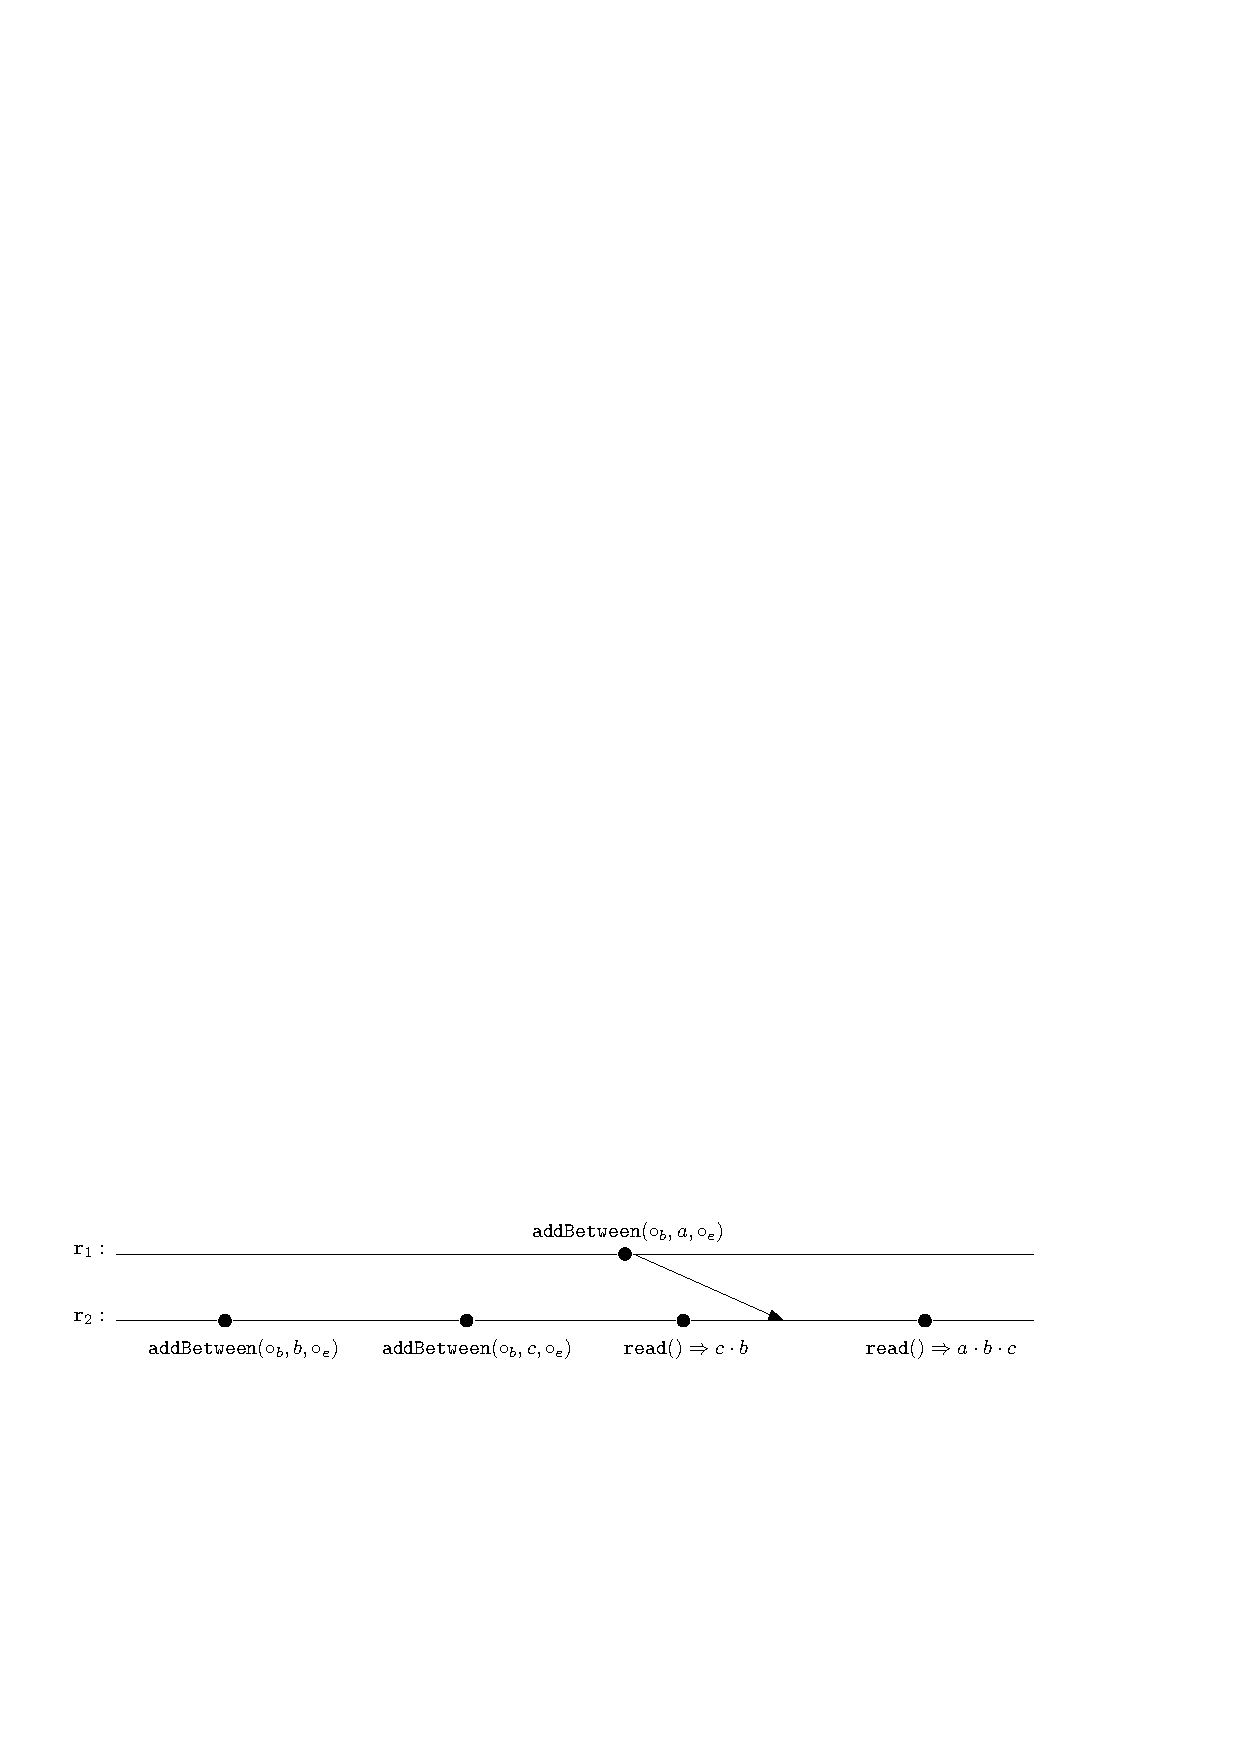
\includegraphics[width=0.85 \textwidth]{figures/ErrorExecutionofWooki.pdf}
\vspace{-10pt}
  \caption{A history w.r.t $\mathit{listBet}_s$ that should be excluded.}
  \label{fig:a wrong history w.r.t listbets}
\end{figure}

Given an execution $e$ of $\aobj$, we propose the following two property of $e$: Given local state $\sigma_1$ and $\sigma_2$ of $e$, if $\sigma_1$ (resp., $\sigma_2$) is obtained from the initial local state by applying a sequence $s_1$ of downstream (resp., a sequence $s_2$ of downstream).

\begin{itemize}
\setlength{\itemsep}{0.5pt}
\item[-] Convergence: if $s_1 \cap \updates = s_2 \cap \updates$, then $\sigma_1 = \sigma_2$.

\item[-] Consistent Conflict Resolution: if $s_1 \cap \updates$ is a sub-sequence of $s_2 \cap \updates$. Let $S$ be the set of downstream of update operations that are in $s_2$ and not in $s_1$, and let $s_3$ be a sequences of $S$ that is consistent with visibility relation. Then, we can obtain $\sigma_2$ from $\sigma_1$ by applying the downstream sequence $s_3$.
\end{itemize}

We say an execution $e$ is ready for downstream, if given a local state $\sigma$ of $e$ which is of replica $\arep$, we can safely apply all the downstream that are still not visible to replica $\arep$ in any order consistent with visibility relation.

Let us go back to \autoref{fig:a wrong history w.r.t listbets}. Let $\sigma_1$ be the local state of $\arep_2$ after we do $\alabelshort[{\tt addBetween}]{\circ_{begin},c,\circ_{end}}$, and let $\sigma_2$ be the local state of $\arep_2$ after we apply the downstream of $\alabelshort[{\tt addBetween}]{\circ_{begin},a,\circ_{end}}$.

$\alabelshort[{\tt addBetween}]{\circ_{begin},c,\circ_{end}}$

$\alabellong[{\tt read}]{}{c \cdot b}{}$,

The following lemma states that, once we prove ready for downstream and downstream of concurrent operations commute, we can obtain convergence and consistent conflict resolution, no matter whether the \Spec{} is deterministic or non-deterministic.

\begin{lemma}
\label{lemma:execution-order linearization ensures convergence and consistent conflict resolution}
If $\aobj$ is \crdtlinearizable{} w.r.t \Spec{} and each of its execution is ready for downstream.
execution-order linearizations

When doing $\alabelshort[{\tt integreteIns}]{c_p,c,c_n}$, for each $i$, $F[i],F[i+1]$ are degree-$d_{min}$-adjacent.
\end{lemma}

\begin {proof}
Obviously, $F[i],F[i+1]$ have degree $d_{min}$, and there is no W-character with degree $d_{min}$ and between $F[i]$ and $F[i+1]$ in $string_s$.

Since $d_{min}$ is the minimal degree of W-characters in $S'$, there does not exists W-character that is between $F[i]$ and $F[i+1]$ and will a degree smaller than $d_{min}$. This completes the proof of this lemma. $\qed$
\end {proof}






\subsection{\crdtlin{} with Non-Deterministic Sequential Specifications}
\label{subsec:appendix RA-linearizability with non-deterministic sequential specifications}

Recall that a sequential specification \Spec{} is deterministic, if for every label, the transition from a given initial state can produce at most one final state. Otherwise, we say that \Spec{} is non-deterministic.

Similarly as in \sectionautorefname \ref{subsec:definition of distributed linearizability}, let us provide the definition of \crdtlin{} with non-deterministic sequential specifications. For presentation reasons, we first consider the case where all the labels in the history are either queries or updates. We say a sequence $s$ is closed under a relation $R$, if when $a$ is in $s$ and $(a,b) \in R$, we have $b$ also in $s$.

\begin{definition}
\label{definition:ralinearizability1 with non-deterministic specifications}
A history $h = (\alabelset,\avisord)$ with $\alabelset\subseteq \queries\cup\updates$ is \crdtlinearizable{} w.r.t. a non-deterministic sequential specification \Spec{}, if there exists a specification sequence $(\alabelset, \aseqord) \in \Spec{}$, called the \emph{\crdtlinearization{}} of $h$, where we remark that the set of labels are identical, such that
\begin{enumerate}[(i)]
\item \aseqord{} is consistent with  \avisord{}, that is: $(\avisord \cup \aseqord)^{+}$ is acyclic,

\item the projection of $\aseqord$ to \emph{updates} is admitted by $\Spec$, i.e. $\aseqord\!\downarrow_{\updates} \in \Spec$,

\item There exists a function $\gconfres: \labels^* \rightarrow \abstates$ (Here the name $\gconfres$ is short for global conflict resolution). Given sequence $s \in \labels^*$, such that $s$ is consistent with $\avisord$ and closed under $\avisord^{-1}$, $\gconfres(s)$ is defined as follows: assume $\abstate_0$ is the initial abstract state of \Spec{},

$$ \gconfres(s)=\left\{
\begin{aligned}
an \ element \ of \ S &  & If \ S = \{ \abstate \vert \abstate_0 \xrightarrow{ \aseqord\!\downarrow_{s\cap \updates} }^* \abstate \} \neq \emptyset \\
undefined & & Otherwise
\end{aligned}
\right.
$$

%$\aseqord\!\downarrow_{s\cap \updates} \in \Spec$

Moreover, we require function $\gconfres$ to satisfy a property called $\mathsf{ConsistentChoice}$:

\begin{itemize}
\setlength{\itemsep}{0.5pt}
\item[-] $\mathsf{ConsistentChoice}$: Given two sub-sequences $s_1,s_2$, such that $s_1$ and $s_2$ are both consistent with $\avisord{}$, $s_1$ and $s_2$ are both closed under $\avisord{}^{-1}$, and $s_1$ is a sub-sequence of $s_2$. Then, $\gconfres(s_1) \xrightarrow{ s_2 - s_1 }^* \gconfres(s_2)$, where $s_2 - s_1$ denotes the sequences obtained from $s_2$ by removing elements of $s_1$.

%$\mathsf{ConsistentChoice}$: Given two sub-sequences $s_1,s_2$ of $\aseqord\!\downarrow_{\updates}$, if $s_2$ contains more operations than $s_1$, and both $\gconfres(s_1)$ and $\gconfres(s_2)$ are defined, then, $\gconfres(s_1) \xrightarrow{ s_2 - s_1 }^* \gconfres(s_2)$, where $s_2 - s_1$ denotes the sequences obtained from $s_2$ by removing elements of $s_1$.
\end{itemize}

\item for each query $\alabel_{\mathsf{qr}}\in \alabelset$, let $s = \avisord^{-1}(\alabel_{\mathsf{qr}})\cap \updates$. Then, we require that $\gconfres(s) \xrightarrow{ \alabel_{\mathsf{qr}} } \gconfres(s)$.
\end{enumerate}
In this case we say that $(\alabelset, \aseqord)$ is an \emph{\crdtlinearization{}} of $h$ w.r.t. $\Spec{}$.
\end{definition}

Let us explain Definition \ref{definition:ralinearizability1 with non-deterministic specifications}. Although $\Spec{}$ is non-deterministic, we use $\gconfres(s)$ to remember our choice for operation sequence $s$. Our definition need to concern two aspects:

\begin{itemize}
\setlength{\itemsep}{0.5pt}
\item[-] Convergence: To obtain $\gconfres(s)$ we only consider $\aseqord\!\downarrow_{s\cap \updates}$, which obviously implies convergence when we consider $\gconfres(s)$ and $\gconfres(s')$ and $s$ is a permutation of $s'$.

\item[-] Unique Choice in Specification: We should get rid of histories that have several operations that use ``Inconsistent non-deterministic choice''.

An example $h$ of such history is shown in \autoref{fig:a wrong history w.r.t listbets}. If only $\alabellong[{\tt read}]{}{c \cdot b}{}$ or $\alabellong[{\tt read}]{}{a \cdot b \cdot c}{}$ exists in $h$, then each of them is reasonable, since $\alabelshort[{\tt remove}]{a_2,a_1,a_3}$ puts $a_1$ in a random position between $a_2$ and $a_3$. However, $\alabellong[{\tt read}]{}{c \cdot b}{}$ represents that $c$ is put before $b$, while $\alabellong[{\tt read}]{}{a \cdot b \cdot c}{}$ represents that $b$ is before $c$. Therefore, we can not put these two $read$ operation in one history.

Since the set of operations visible to $\alabellong[{\tt read}]{}{c \cdot b}{}$ and the set of operations visible to $\alabellong[{\tt read}]{}{a \cdot b \cdot c}{}$ are different, our convergence requirement is not enough to rule them out. Instead, the $\mathsf{ConsistentChoice}$ condition is able to rule them out. $\mathsf{ConsistentChoice}$ essentially represents that, a ``bigger state'' follows the same choice in a ``smaller'' state.
\end{itemize}

\begin{figure}[t]
  \centering
  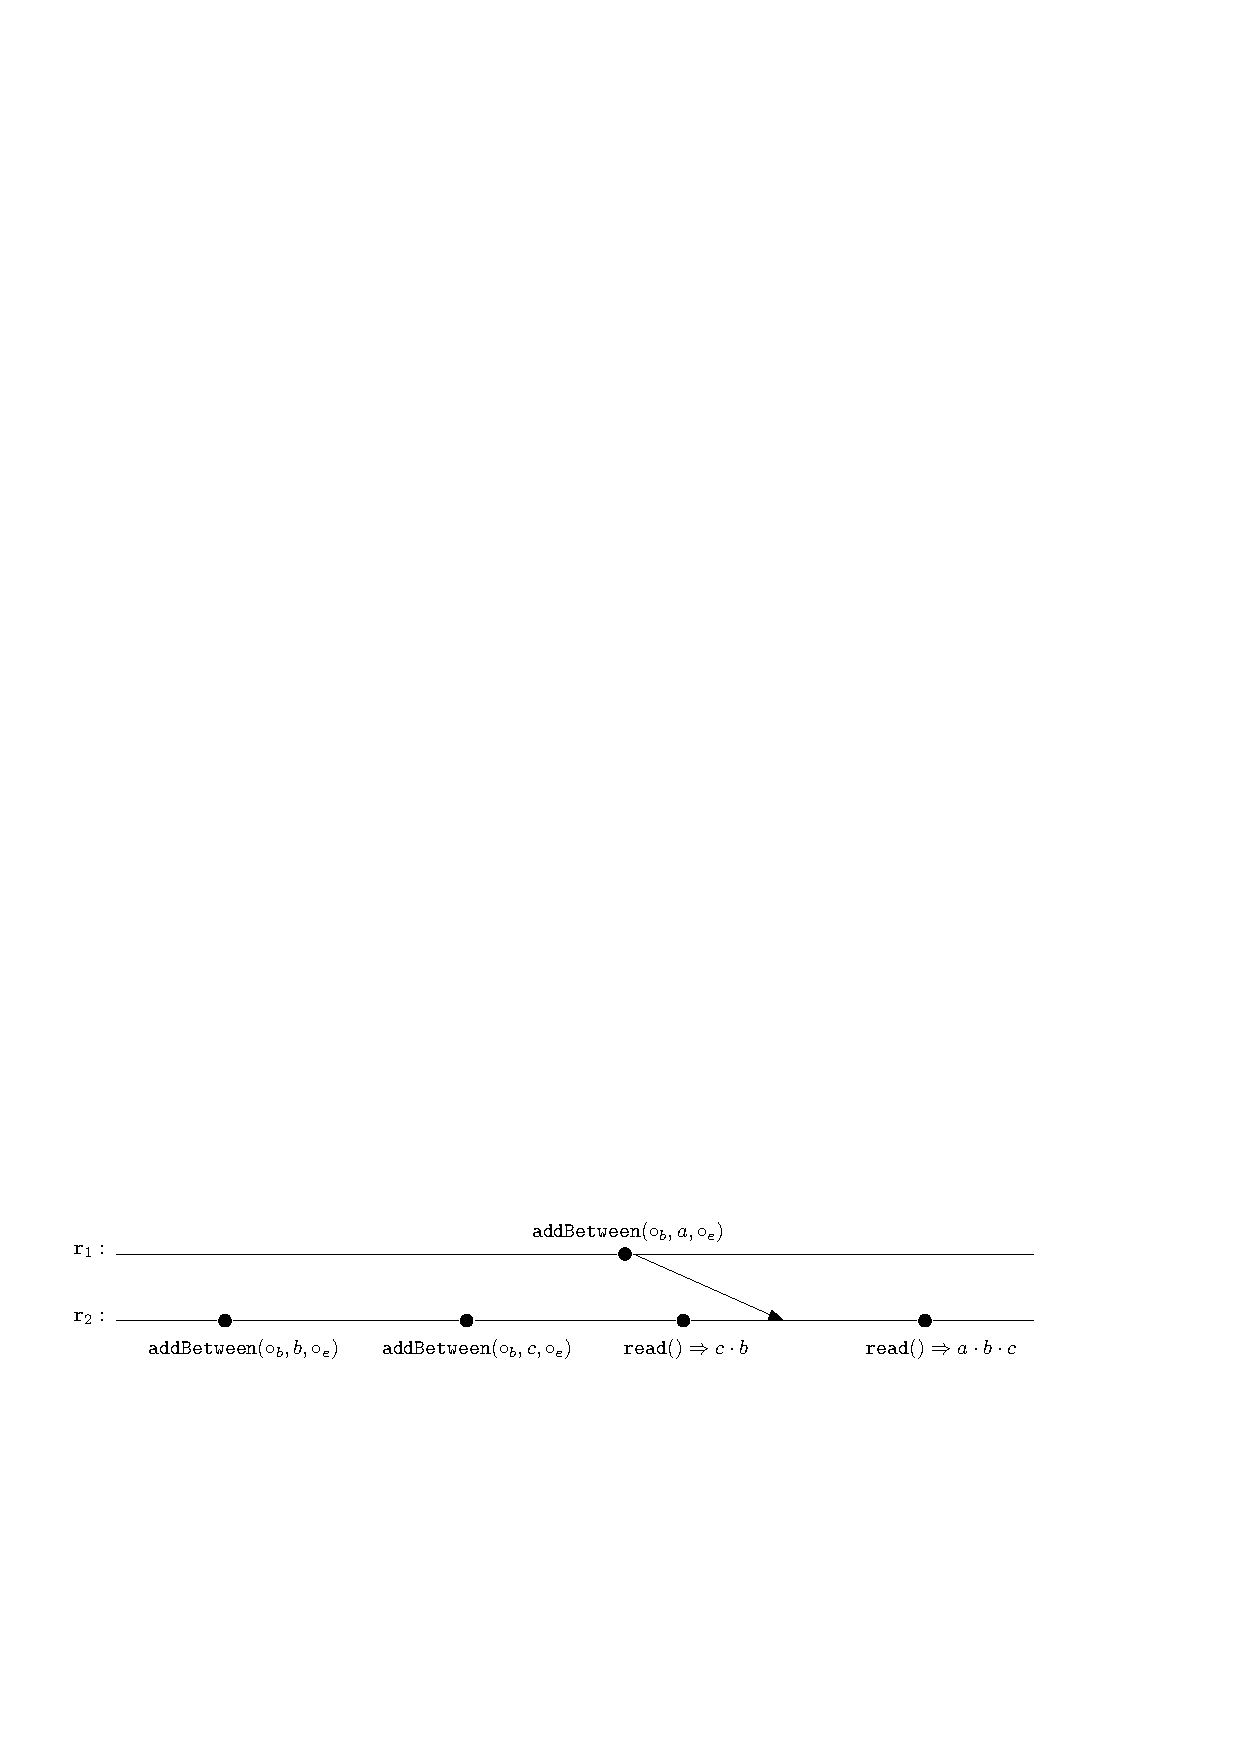
\includegraphics[width=0.85 \textwidth]{figures/ErrorExecutionofWooki.pdf}
\vspace{-10pt}
  \caption{A ``wrong'' history w.r.t $\mathit{listBet}_s$.}
  \label{fig:a wrong history w.r.t listbets}
\end{figure}


%Since the sequential specification is non-deterministic, for each operation sequence $s$, we fix $\gconfres(s)$ to be the consequence in sequential specification when applying update operations in $s$ according to \aseqord{} order from the initial abstract state $\abstate_0$ of sequential specification. The condition of $\gconfres(s_1) \xrightarrow{ s_2 - s_1 }^* \gconfres(s_2)$utf ensures that, the conflict resolution of bigger state $\gconfres(s_2)$ should also respect the conflict resolution of smaller state $\gconfres(s_1)$. Or we cam say, $\gconfres(s_1)$ is a ``sub-state'' of $\gconfres(s_2)$.

The case when histories include query-updates is similarly dealt with as Definition \ref{definition:distributed linearizability}. We do it by rewriting of the original history where each query-update is decomposed into a label representing the query part and another label representing the update part.

\begin{definition}[\CRDTLin{} with Non-Deterministic Sequential Specifications]
\label{definition:ralinearizability with non-deterministic sequential specifications and rewritting}
A history $h =(\alabelset,\avisord)$ is \crdtlinearizable{} w.r.t. a non-deterministic sequential specification \Spec{}, if there exists a query-update rewriting $\gamma$ such that $\gamma(h)$ is \crdtlinearizable{} w.r.t. \Spec{}.
\end{definition}

A set $H$ of histories is called \crdtlinearizable{} w.r.t a non-deterministic sequential specification $\Spec$ when each history $h\in H$ is \crdtlinearizable{} w.r.t. $\Spec$. A data type implementation is \crdtlinearizable{} w.r.t. a non-deterministic sequential specification $\Spec$ if for any object $\aobj$ of the data type, the set $\histories(\aobj)$ is linearizable w.r.t. $\Spec$.

Let us begin to consider convergence. Given a \crdtlinearizable{} history with two replicas $r_1,r_2$ see the same set of operations. According to Definition \ref{definition:ralinearizability1 with non-deterministic specifications} and Definition \ref{definition:ralinearizability with non-deterministic sequential specifications and rewritting}, to obtain $\gconfres(s)$, we only consider $\aseqord\!\downarrow_{s\cap \updates}$, which obviously implies convergence, as formalized in the following lemma.

\begin{lemma}
\label{lemma:distributed linarizability implies convergence for non-deterministic sequential specifications}
If a history $h$ is \crdtlinearizable{} w.r.t. a non-deterministic sequential specification \Spec, then $h$ is convergent.
\end{lemma}






\subsection{Proof Methodology for \crdtlin{} w.r.t Non-Deterministic Sequential Specifications}
\label{subsec:appendix proof methodology for RA-linearizability w.r.t non-deterministic sequential specifications}

In this subsection, we propose our methodology for proving \crdtlin{} w.r.t non-deterministic sequential specifications. Our methodology is similar for proving \crdtlin{} w.r.t deterministic sequential specifications in \sectionautorefname \ref{ssec:proof-methodology}.

%The similar points are as follows:

%\begin{itemize}
%\item[-] We still instrument the object semantics with an auxiliary variable $\alinord$ recording a linearization of the current history. %Only the execution of an \lstinline|atSource| portion of an operation engenders the extension of $\alinord$ by adding the current operation at some specific position. To guarantee that the linearization is consistent with the visibility relation, the operation must be inserted in the linearization after all the operations which are visible at the replica executing \lstinline|atSource|.

%\item[-] We still need to prove the property $\mathsf{ReplicaStates}$ and $\mathsf{\CRDTLinshort{}}$.

    %\begin{itemize}
    %\item[-] $\mathsf{ReplicaStates}$: requiring that for each replica $\arep$ with local configuration $(\alabelset,\astate)$, the state $\sigma$ is obtained by applying the downstreams of the operations in $\alabelset$ (that have been delivered to $\arep$) in the order defined by $\alinord$, and

    %\item[-] $\mathsf{\CRDTLinshort{}}$: requiring that the sequence $\alinord$ is an \crdtlinearization{} of the current history (w.r.t. $\Spec{}$).
    %\end{itemize}

%\item[-] We still rely on additional assertions describing the effect of each downstream.

%\item[-] We still need to prove $\mathsf{Refinement}$. The proof of $\mathsf{Refinement}$ still relies on a refinement mapping between replica states and states of the specification, denoted by $\refmap$.

    %\begin{itemize}
    %\item[-] $\mathsf{Refinement}$: each downstream produced by an update $\alabel$ and respectively, each query $\alabel$, is simulated by the application of $\alabel$ in the specification $\Spec$.
    %\end{itemize}
%\end{itemize}

Additionally, we need the following definitions:

\begin{itemize}
\setlength{\itemsep}{0.5pt}
\item[-] We introduce a function $\igconfres: \labels^* \rightarrow \states$ to explicitly record the consequence of applying downstream.

Given a sequence $s$ of downstream, such that $s$ is consistent with $\avisord$ and closed under $\avisord^{-1}$, $\igconfres(s)$ is the local state obtained by applying downstream of $s$ in the order of $s$.

\item[-] From $\igconfres(s)$, we generate a abstract state $\gconfres'(s)$. Latter we will prove that $\gconfres'$ satisfies the requirement of $\gconfres$.

    We use a refinement mapping $\refmap$ that maps $\igconfres(s)$ into $\gconfres'(s)$. %Or we can say, $\refmap{}(\igconfres(s)) = \gconfres(s)$.
\end{itemize}

%$\igconfres(s)$ may be undefined for some sequence $s$, for example, apply the downstream of $\alabelshort[{\tt remove}]{a}$ when no downstream of inserting $a$ has been applied.

Here the name $\igconfres$ is short for global conflict resolution in implementations.

Then, we need to prove the following properties:

\begin{itemize}
\setlength{\itemsep}{0.5pt}
\item[-] We prove that any two downstream that correspond to two ``concurrent'' operations commute.

\item[-] We prove $\mathsf{Refinement}$ holds between $\igconfres(s)$ and $\gconfres'(s)$ in a way as follows:

\begin{enumerate}
\item Given an update operation $\alabel$, if $s \cdot \alabel$ is consistent with $\avisord$ and closed under $\avisord^{-1}$, obviously $\igconfres(s \cdot \alabel)$ is obtained from $\igconfres(s)$ by applying the downstream of $\alabel$. Then, we require that $\gconfres'(s)\xRightarrow{\alabel}\gconfres'(s \cdot \alabel)$.

\item If a query $\alabel$ is applied on a state $\igconfres(s)$ or it is introduced by a rewriting of a query-update that executes \lstinline|atSource| on a state $\igconfres(s)$, then $\gconfres'(s)\xRightarrow{\alabel}\gconfres'(s)$.
\end{enumerate}
\end{itemize}

With above definitions and properties, our proof proceed as follows:

\noindent {\bf Prove correctness of $\gconfres'$:} We prove that $\gconfres'$ satisfies the requirement of $\gconfres$ as follows:

\begin{itemize}
\setlength{\itemsep}{0.5pt}
\item[-] Given sequences $s_1$ and $s_2$, such that both $s_1$ and $s_2$ are consistent with $\avisord$ and are closed under $\avisord^{-1}$, and $s_1$ is a permutation of $s_2$. Then, since any two downstream that correspond to two ``concurrent'' operations commute, we can see that $\igconfres(s_1)$ = $\igconfres(s_2)$. Since $\mathsf{Refinement}$ holds, we have transitions $\gconfres'(\epsilon)\xRightarrow{s_1}^*\gconfres'(s_1)$ and $\gconfres'(\epsilon)\xRightarrow{s_2}^*\gconfres'(s_2)$. Thus, $\gconfres'(s_1) = \gconfres'(s_2)$.

    Moreover, let $s_3$ be the projection of $\alinord$ into operations of $s_1$. Similarly, we can prove that $\gconfres'(s_1) = \gconfres'(s_3)$.

\item[-] $\mathsf{ConsistentChoice}$: Given $s_1$ and $s_2$, such that they are both consistent with $\avisord$ and closed under $\avisord^{-1}$, and $s_1$ is a sub-sequence of $s_2$. Obviously $s_1 \cdot (s_2 - s_1)$ is closed under $\avisord^{-1}$.

    We prove that $s_1 \cdot (s_2 - s_1)$ is consistent with $\avisord$ by contradiction. Assume that $s_1 \cdot (s_2 - s_1)$ is not consistent with $\avisord$. Since $s_1$ and $s_2$ are consistent with $\avisord$, this implies that, there exists $a,b$, such that, $a \in s_1$, $b \in s_2 - s_1$, and $(b,a) \in \avisord$. Or we can say, $(b,a) \in \avisord^{-1}$, $a \in s_1$, $b \notin s_1$. This contradicts the assumption that $s_1$ is closed under $\avisord^{-1}$. Therefore, $s_1 \cdot (s_2 - s_1)$ is consistent with $\avisord$.

    Since $s_2$ and $s_1 \cdot (s_2 - s_1)$ are consistent with $\avisord$ and closed under $\avisord^{-1}$, we know that there exists $\igconfres(s_2)$ and $\igconfres(s_1 \cdot (s_2 - s_1))$, and transitions from $\igconfres(\epsilon)$ to $\igconfres(s_2)$, and transitions from $\igconfres(\epsilon)$ to $\igconfres(s_1 \cdot (s_2 - s_1))$. By $\mathsf{Refinement}$, we know that there exist transitions $\gconfres'(\epsilon)\xRightarrow{s_2}^*\gconfres'(s_2)$ and transitions $\gconfres'(\epsilon)\xRightarrow{s_1}^*\gconfres'(s_1)\xRightarrow{s_2 - s_1}^*\gconfres'(s_1 \cdot (s_2 - s_1))$.

    Obviously, $s_2$ is a permutation of $s_1 \cdot (s_2 - s_1)$. As discussed above, we can see that $\gconfres'(s_2) = \gconfres'(s_1 \cdot (s_2 - s_1))$.
\end{itemize}

\noindent {\bf Prove $\mathsf{ReplicaStates}$:} $\mathsf{ReplicaStates}$ holds since any two downstream that correspond to two ``concurrent'' operations commute.

\noindent {\bf Prove $\mathsf{Refinement}$:} This is specific to implementations.

\noindent {\bf Prove Annotations:} If above proof relies on annotations of the downstream or local state, then we should also prove that the annotation of downstream holds for new downstream, and the annotation of local state holds for new local state.

\noindent {\bf Prove $\mathsf{\CRDTLinshort{}}$:} Similarly as in \sectionautorefname \ref{ssec:proof-methodology}, this is a consequence of $\mathsf{ReplicaStates}$, $\mathsf{Refinement}$, and the correctness of $\gconfres'$.


We have applied this methodology to Wooki and Tree-Doc. For Wooki and Tree-Doc, we use execution-order linearizations. The linearization $\alinord$ is defined by the order in which the \lstinline|atSource| procedures are executed.










\subsection{Proof of Wooki}
\label{subsec:proof of Wooki}




Then, let us prove that Wooki is \crdtlinearizable{} w.r.t $\mathit{listBet}_s$.

\begin{lemma}
\label{lemma:Wooki is correct}
Wooki is \crdtlinearizable{} w.r.t $\mathit{listBet}_s$.
\end{lemma}

\begin {proof}

We prove following the prove methodology of \sectionautorefname \ref{subsec:appendix proof methodology for RA-linearizability w.r.t non-deterministic sequential specifications}.

We define abstract state $\gconfres'(s)$ as follows: given a sequence $s$ of downstream, such that $s$ is consistent with $\avisord$ and closed under $\avisord^{-1}$, assume $\igconfres(s) = c_1 \dot \ldots \cdot c_n$, where for each $i$, $c_i = (id_i,v_i,degree_i,flag_i)$. Then, $\gconfres'(s) = (v_1 \cdot \ldots \cdot v_n,T)$, where $T = \{ v_i \vert flag_i = \mathit{false} \}$.

Then, let us prove the downstream of concurrent operations commute and the $\mathsf{Refinement}$ property,

\begin{itemize}
\setlength{\itemsep}{0.5pt}
\item[-] By Lemma \ref{lemma:in Wooki algorithm, two downstreams of two addBetween operations commute}, we can see that the downstream of concurrent {\tt addBetween} operations commute. According to Wooki algorithm, it is easy to see that the downstream of concurrent {\tt remove} operations commute, since they both put some value into tombstone; A {\tt addBetween} and a {\tt remove} downstream commute when they are concurrent because in this case, the W-character removed by {\tt remove} are different from the pair added by the {\tt addBetween}.
\item[-] Let us prove $\mathsf{Refinement}$ holds between $\igconfres(s)$ and $\gconfres'(s)$ as follows:

    \begin{itemize}
    \setlength{\itemsep}{0.5pt}
    \item[-] Given an operation $\alabel = \alabelshort[{\tt addBetween}]{a,b,c}$, assume that $s \cdot \alabel$ is consistent with $\avisord$ and closed under $\avisord^{-1}$. We need to prove that $\gconfres'(s)\xRightarrow{\alabel}\gconfres'(s \cdot \alabel)$.

        Assume that $\igconfres(s)=str_1$, and $\igconfres(s')=str_2$. We can see that there exists W-character $c_a = (\_,a,\_,\_)$ and $c_c = (\_,c,\_,\_)$ in $str_1$, such that $c_a$ is before $c_c$ in $str_1$, there is no W-character of value $b$ in $str_1$, and $str_2$ is obtained from $str_1$ by inserting a W-character $c_b = (\_,b,\_,\mathit{true})$ at some position between $c_a$ and $c_c$. Then, it is easy to see that $\gconfres'(s)\xRightarrow{\alabel}\gconfres'(s \cdot \alabel)$.

    \item[-] Given an operation $\alabel = \alabelshort[{\tt remove}]{b}$, assume that $s \cdot \alabel$ is consistent with $\avisord$ and closed under $\avisord^{-1}$. We need to prove that $\gconfres'(s)\xRightarrow{\alabel}\gconfres'(s \cdot \alabel)$.

        Assume that $\igconfres(s)=str_1$, and $\igconfres(s')=str_2$. We can see that there exists W-character $c_b = (\_,b,\_,\_)$ in $str_1$, and $str_2$ is obtained from $str_1$ by setting the flag of $c_b$ into $\mathit{false}$. Then, it is easy to see that $\gconfres'(s)\xRightarrow{\alabel}\gconfres'(s \cdot \alabel)$.

    \item[-] Given an operation $\alabel = \alabellong[{\tt read}]{}{s_1}{}$, assume that $s \cdot \alabel$ is consistent with $\avisord$ and closed under $\avisord^{-1}$. Assume that $\alabel$ is applied on the state $\igconfres(s)$. We need to prove that $\gconfres'(s)\xRightarrow{\alabel}\gconfres'(s)$.

        Assume that $\igconfres(s)=c_1 \cdot \ldots \cdot c_n$, where for each $i$, $c_i = (id_i,v_i,degree_i,flag_i)$. Then, $s_1$ is obtained from $v_1 \cdot \ldots \cdot v_n$ by removing values with flag $\mathit{false}$. Then, it is easy to see that $\gconfres'(s)\xRightarrow{\alabel}\gconfres'(s)$.
    \end{itemize}

\end{itemize}

Then, our proof proceeds as follows:

\begin{itemize}
\setlength{\itemsep}{0.5pt}
\item[-] {\bf Prove correctness of $\gconfres'$:} With above properties, as discussed in \sectionautorefname \ref{subsec:appendix proof methodology for RA-linearizability w.r.t non-deterministic sequential specifications}, we can prove that $\gconfres'$ satisfies the requirement of $\gconfres$ in Definition \ref{definition:ralinearizability1 with non-deterministic specifications}.

\item[-] {\bf Prove $\mathsf{ReplicaStates}$:} Since every operation is appended to the linearization when it executes {\tt atSource} it clearly follows, the linearization order is consistent with visibility order. Then, by the {\textred{causal delivery}} assumption, the order in which downstream are applied at a given replica is also consistent with the visibility order. Let $\alinord_1$ be the projection of linearization order into labels applied in a replica $\arep$, and $\alinord_2$ be the order of labels applied in replica $\arep$. By Lemma \ref{lemma:given two sequence consistent with visibility order, one can be obtained from the other}, $\alinord_2$ can be obtained from $\alinord_1$ by several time of swapping adjacent pair of concurrent operations. This holds, since we have already prove that, the downstream of concurrent operations commute.

\item[-] {\bf Prove $\mathsf{\CRDTLinshort{}}$:} Finally, we describe the proof of the fact that $\mathsf{\CRDTLinshort{}}$ is an inductive invariant. As already mentioned, appending operations to the linearization when they execute \lstinline|atSource| clearly implies that $\alinord$ is consistent with the visibility. Next, the projection of $\alinord$ on the updates is obviously admitted by the specification (the updates are always enabled from the point of view of the specification).
We also have to argue that for each query $\alabel_{\mathsf{qr}} = \alabellongind[read]{}{s_1}{}$, the sequence $\alinord'\cdot \alabel_{\mathsf{qr}}$ where $\alinord'$ is the projection of $\alinord$ on the set of updates
visible to $\alabel_{\mathsf{qr}}$ is admitted by the specification. First, by $\mathsf{ReplicaStates}$, the state $\sigma$ of the replica where $\alabel_{\mathsf{qr}}$ is applied is obtained by applying the downstream of the operations visible to $\alabel_{\mathsf{qr}}$ in the linearization order. Then, by $\mathsf{Refinement}$, every downstream is simulated by the corresponding operation in the context of the specification. This implies that $\gconfres'(\epsilon)\xRightarrow{\alinord'}^*\gconfres'(\alinord')$. The query $\alabel_{\mathsf{qr}}$ is also simulated by the same operation in the context of the specification, which implies that $\gconfres'(\alinord')\xRightarrow{\alabel_{\mathsf{qr}}}\gconfres'(\alinord')$. These two facts imply that $\gconfres'(\epsilon)\xRightarrow{\alinord'\cdot \alabel_{\mathsf{qr}}}^*\gconfres'(\alinord')$ which means that $\alinord'\cdot \alabel_{\mathsf{qr}}$ is admitted by the specification.
\end{itemize}

This completes the proof of this lemma. $\qed$
\end {proof}
}































\forget
{
\section{\crdtlin{} with Non-Deterministic Sequential Specifications and Its Proof}
\label{sec:appendix RA-linearizability with non-deterministic sequential specifications and its proof}



\subsection{\crdtlin{} with Non-Deterministic Sequential Specifications}
\label{subsec:appendix RA-linearizability with non-deterministic sequential specifications}

Recall that a sequential specification \Spec{} is deterministic, if for every label, the transition from a given initial state can produce at most one final state. Otherwise, we say that \Spec{} is non-deterministic.

Similarly as in \sectionautorefname \ref{subsec:definition of distributed linearizability}, let us provide the definition of \crdtlin{} with non-deterministic sequential specifications. For presentation reasons, we first consider the case where all the labels in the history are either queries or updates. We say a sequence $s$ is closed under a relation $R$, if when $a$ is in $s$ and $(a,b) \in R$, we have $b$ also in $s$.

\begin{definition}
\label{definition:ralinearizability1 with non-deterministic specifications}
A history $h = (\alabelset,\avisord)$ with $\alabelset\subseteq \queries\cup\updates$ is \crdtlinearizable{} w.r.t. a non-deterministic sequential specification \Spec{}, if there exists a specification sequence $(\alabelset, \aseqord) \in \Spec{}$, called the \emph{\crdtlinearization{}} of $h$, where we remark that the set of labels are identical, such that
\begin{enumerate}[(i)]
\item \aseqord{} is consistent with  \avisord{}, that is: $(\avisord \cup \aseqord)^{+}$ is acyclic,

\item the projection of $\aseqord$ to \emph{updates} is admitted by $\Spec$, i.e. $\aseqord\!\downarrow_{\updates} \in \Spec$,

\item There exists a function $\gconfres: \labels^* \rightarrow \abstates$ (Here the name $\gconfres$ is short for global conflict resolution). Given sequence $s \in \labels^*$, such that $s$ is consistent with $\avisord$ and closed under $\avisord^{-1}$, $\gconfres(s)$ is defined as follows: assume $\abstate_0$ is the initial abstract state of \Spec{},

$$ \gconfres(s)=\left\{
\begin{aligned}
an \ element \ of \ S &  & If \ S = \{ \abstate \vert \abstate_0 \xrightarrow{ \aseqord\!\downarrow_{s\cap \updates} }^* \abstate \} \neq \emptyset \\
undefined & & Otherwise
\end{aligned}
\right.
$$

%$\aseqord\!\downarrow_{s\cap \updates} \in \Spec$

Moreover, we require function $\gconfres$ to satisfy a property called $\mathsf{ConsistentChoice}$:

\begin{itemize}
\setlength{\itemsep}{0.5pt}
\item[-] $\mathsf{ConsistentChoice}$: Given two sub-sequences $s_1,s_2$, such that $s_1$ and $s_2$ are both consistent with $\avisord{}$, $s_1$ and $s_2$ are both closed under $\avisord{}^{-1}$, and $s_1$ is a sub-sequence of $s_2$. Then, $\gconfres(s_1) \xrightarrow{ s_2 - s_1 }^* \gconfres(s_2)$, where $s_2 - s_1$ denotes the sequences obtained from $s_2$ by removing elements of $s_1$.

%$\mathsf{ConsistentChoice}$: Given two sub-sequences $s_1,s_2$ of $\aseqord\!\downarrow_{\updates}$, if $s_2$ contains more operations than $s_1$, and both $\gconfres(s_1)$ and $\gconfres(s_2)$ are defined, then, $\gconfres(s_1) \xrightarrow{ s_2 - s_1 }^* \gconfres(s_2)$, where $s_2 - s_1$ denotes the sequences obtained from $s_2$ by removing elements of $s_1$.
\end{itemize}

\item for each query $\alabel_{\mathsf{qr}}\in \alabelset$, let $s = \avisord^{-1}(\alabel_{\mathsf{qr}})\cap \updates$. Then, we require that $\gconfres(s) \xrightarrow{ \alabel_{\mathsf{qr}} } \gconfres(s)$.
\end{enumerate}
In this case we say that $(\alabelset, \aseqord)$ is an \emph{\crdtlinearization{}} of $h$ w.r.t. $\Spec{}$.
\end{definition}

Let us explain Definition \ref{definition:ralinearizability1 with non-deterministic specifications}. Although $\Spec{}$ is non-deterministic, we use $\gconfres(s)$ to remember our choice for operation sequence $s$. Our definition need to concern two aspects:

\begin{itemize}
\setlength{\itemsep}{0.5pt}
\item[-] Convergence: To obtain $\gconfres(s)$ we only consider $\aseqord\!\downarrow_{s\cap \updates}$, which obviously implies convergence when we consider $\gconfres(s)$ and $\gconfres(s')$ and $s$ is a permutation of $s'$.

\item[-] Unique Choice in Specification: We should get rid of histories that have several operations that use ``Inconsistent non-deterministic choice''.

An example $h$ of such history is shown in \autoref{fig:a wrong history w.r.t listbets}. If only $\alabellong[{\tt read}]{}{c \cdot b}{}$ or $\alabellong[{\tt read}]{}{a \cdot b \cdot c}{}$ exists in $h$, then each of them is reasonable, since $\alabelshort[{\tt remove}]{a_2,a_1,a_3}$ puts $a_1$ in a random position between $a_2$ and $a_3$. However, $\alabellong[{\tt read}]{}{c \cdot b}{}$ represents that $c$ is put before $b$, while $\alabellong[{\tt read}]{}{a \cdot b \cdot c}{}$ represents that $b$ is before $c$. Therefore, we can not put these two $read$ operation in one history.

Since the set of operations visible to $\alabellong[{\tt read}]{}{c \cdot b}{}$ and the set of operations visible to $\alabellong[{\tt read}]{}{a \cdot b \cdot c}{}$ are different, our convergence requirement is not enough to rule them out. Instead, the $\mathsf{ConsistentChoice}$ condition is able to rule them out. $\mathsf{ConsistentChoice}$ essentially represents that, a ``bigger state'' follows the same choice in a ``smaller'' state.
\end{itemize}

\begin{figure}[t]
  \centering
  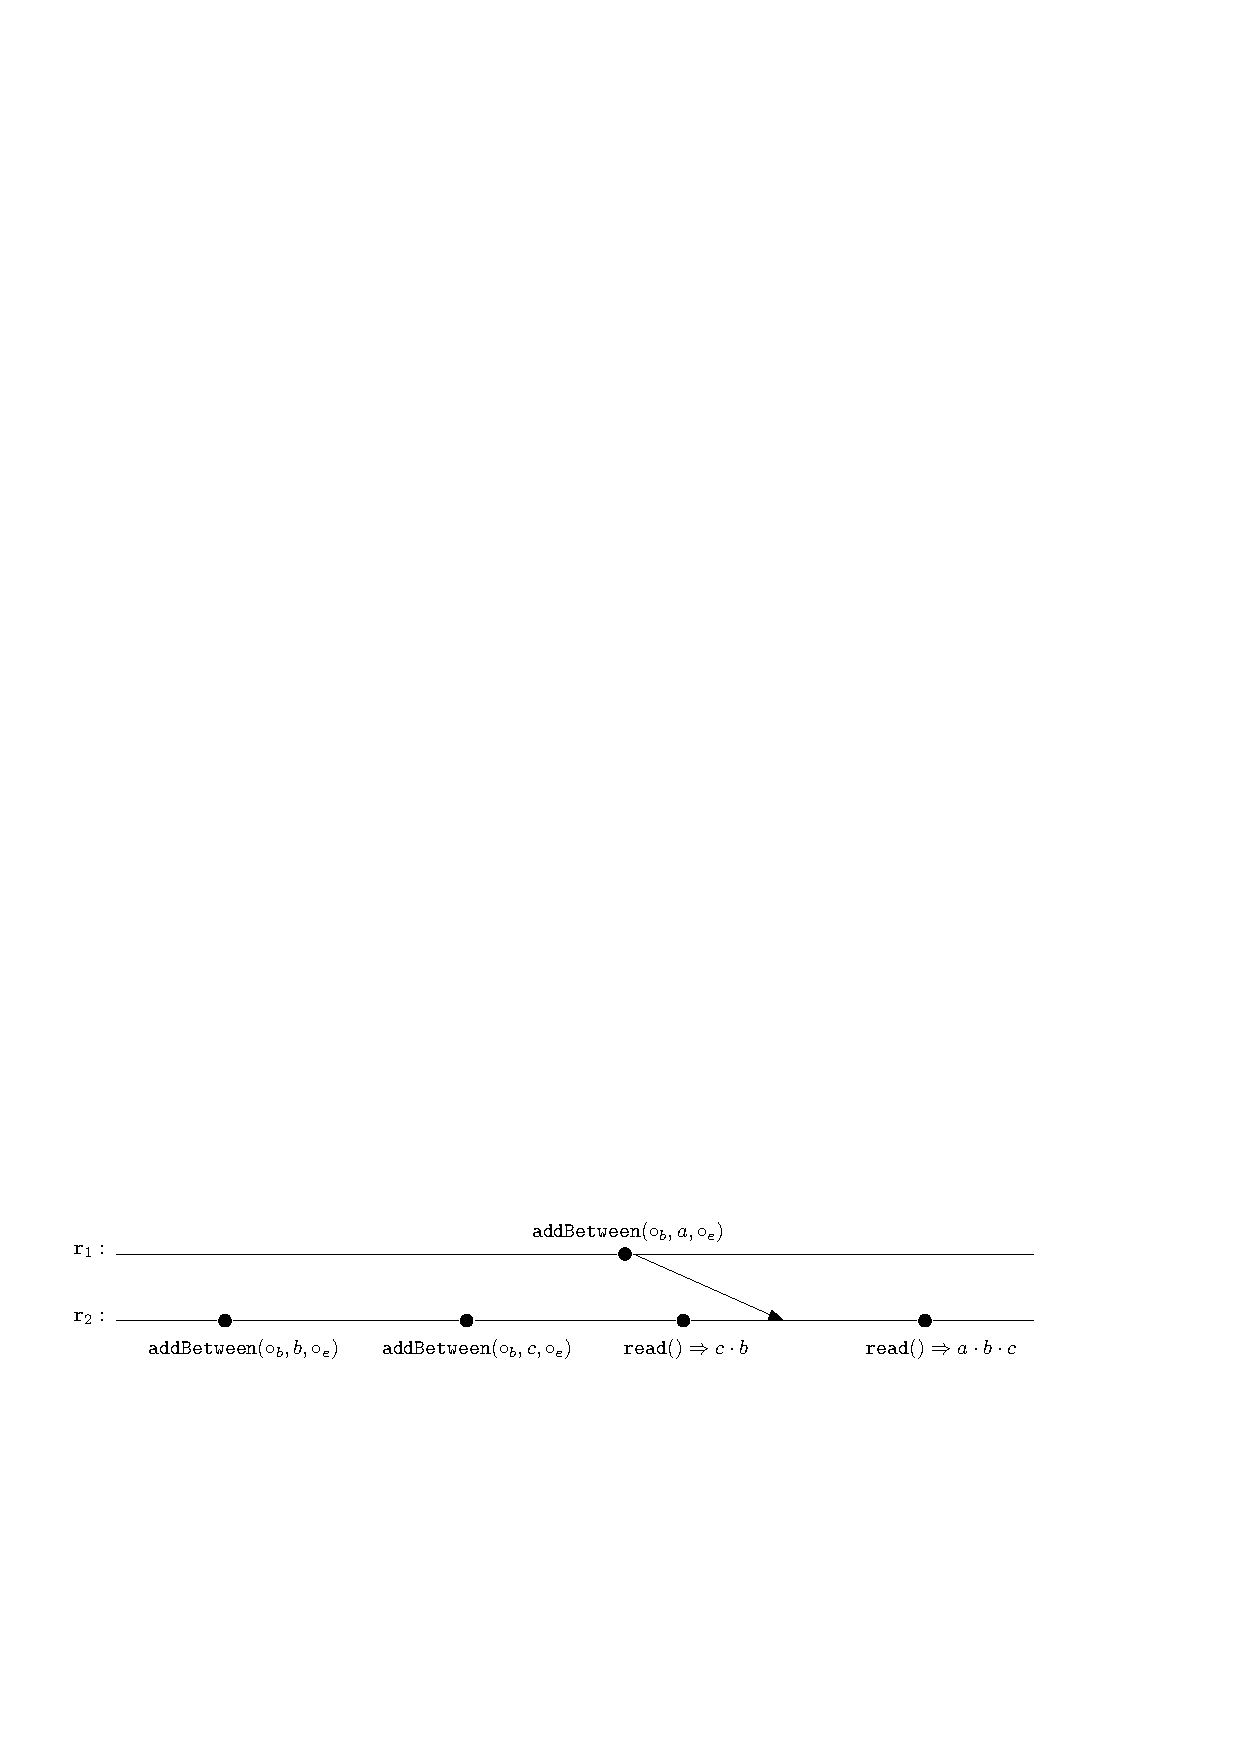
\includegraphics[width=0.85 \textwidth]{figures/ErrorExecutionofWooki.pdf}
\vspace{-10pt}
  \caption{A ``wrong'' history w.r.t $\mathit{listBet}_s$.}
  \label{fig:a wrong history w.r.t listbets}
\end{figure}


%Since the sequential specification is non-deterministic, for each operation sequence $s$, we fix $\gconfres(s)$ to be the consequence in sequential specification when applying update operations in $s$ according to \aseqord{} order from the initial abstract state $\abstate_0$ of sequential specification. The condition of $\gconfres(s_1) \xrightarrow{ s_2 - s_1 }^* \gconfres(s_2)$utf ensures that, the conflict resolution of bigger state $\gconfres(s_2)$ should also respect the conflict resolution of smaller state $\gconfres(s_1)$. Or we cam say, $\gconfres(s_1)$ is a ``sub-state'' of $\gconfres(s_2)$.

The case when histories include query-updates is similarly dealt with as Definition \ref{definition:distributed linearizability}. We do it by rewriting of the original history where each query-update is decomposed into a label representing the query part and another label representing the update part.

\begin{definition}[\CRDTLin{} with Non-Deterministic Sequential Specifications]
\label{definition:ralinearizability with non-deterministic sequential specifications and rewritting}
A history $h =(\alabelset,\avisord)$ is \crdtlinearizable{} w.r.t. a non-deterministic sequential specification \Spec{}, if there exists a query-update rewriting $\gamma$ such that $\gamma(h)$ is \crdtlinearizable{} w.r.t. \Spec{}.
\end{definition}

A set $H$ of histories is called \crdtlinearizable{} w.r.t a non-deterministic sequential specification $\Spec$ when each history $h\in H$ is \crdtlinearizable{} w.r.t. $\Spec$. A data type implementation is \crdtlinearizable{} w.r.t. a non-deterministic sequential specification $\Spec$ if for any object $\aobj$ of the data type, the set $\histories(\aobj)$ is linearizable w.r.t. $\Spec$.

Let us begin to consider convergence. Given a \crdtlinearizable{} history with two replicas $r_1,r_2$ see the same set of operations. According to Definition \ref{definition:ralinearizability1 with non-deterministic specifications} and Definition \ref{definition:ralinearizability with non-deterministic sequential specifications and rewritting}, to obtain $\gconfres(s)$, we only consider $\aseqord\!\downarrow_{s\cap \updates}$, which obviously implies convergence, as formalized in the following lemma.

\begin{lemma}
\label{lemma:distributed linarizability implies convergence for non-deterministic sequential specifications}
If a history $h$ is \crdtlinearizable{} w.r.t. a non-deterministic sequential specification \Spec, then $h$ is convergent.
\end{lemma}






\subsection{Proof Methodology for \crdtlin{} w.r.t Non-Deterministic Sequential Specifications}
\label{subsec:appendix proof methodology for RA-linearizability w.r.t non-deterministic sequential specifications}

In this subsection, we propose our methodology for proving \crdtlin{} w.r.t non-deterministic sequential specifications. Our methodology is similar for proving \crdtlin{} w.r.t deterministic sequential specifications in \sectionautorefname \ref{ssec:proof-methodology}.

%The similar points are as follows:

%\begin{itemize}
%\item[-] We still instrument the object semantics with an auxiliary variable $\alinord$ recording a linearization of the current history. %Only the execution of an \lstinline|atSource| portion of an operation engenders the extension of $\alinord$ by adding the current operation at some specific position. To guarantee that the linearization is consistent with the visibility relation, the operation must be inserted in the linearization after all the operations which are visible at the replica executing \lstinline|atSource|.

%\item[-] We still need to prove the property $\mathsf{ReplicaStates}$ and $\mathsf{\CRDTLinshort{}}$.

    %\begin{itemize}
    %\item[-] $\mathsf{ReplicaStates}$: requiring that for each replica $\arep$ with local configuration $(\alabelset,\astate)$, the state $\sigma$ is obtained by applying the downstreams of the operations in $\alabelset$ (that have been delivered to $\arep$) in the order defined by $\alinord$, and

    %\item[-] $\mathsf{\CRDTLinshort{}}$: requiring that the sequence $\alinord$ is an \crdtlinearization{} of the current history (w.r.t. $\Spec{}$).
    %\end{itemize}

%\item[-] We still rely on additional assertions describing the effect of each downstream.

%\item[-] We still need to prove $\mathsf{Refinement}$. The proof of $\mathsf{Refinement}$ still relies on a refinement mapping between replica states and states of the specification, denoted by $\refmap$.

    %\begin{itemize}
    %\item[-] $\mathsf{Refinement}$: each downstream produced by an update $\alabel$ and respectively, each query $\alabel$, is simulated by the application of $\alabel$ in the specification $\Spec$.
    %\end{itemize}
%\end{itemize}

Additionally, we need the following definitions:

\begin{itemize}
\setlength{\itemsep}{0.5pt}
\item[-] We introduce a function $\igconfres: \labels^* \rightarrow \states$ to explicitly record the consequence of applying downstream.

Given a sequence $s$ of downstream, such that $s$ is consistent with $\avisord$ and closed under $\avisord^{-1}$, $\igconfres(s)$ is the local state obtained by applying downstream of $s$ in the order of $s$.

\item[-] From $\igconfres(s)$, we generate a abstract state $\gconfres'(s)$. Latter we will prove that $\gconfres'$ satisfies the requirement of $\gconfres$.

    We use a refinement mapping $\refmap$ that maps $\igconfres(s)$ into $\gconfres'(s)$. %Or we can say, $\refmap{}(\igconfres(s)) = \gconfres(s)$.
\end{itemize}

%$\igconfres(s)$ may be undefined for some sequence $s$, for example, apply the downstream of $\alabelshort[{\tt remove}]{a}$ when no downstream of inserting $a$ has been applied.

Here the name $\igconfres$ is short for global conflict resolution in implementations.

Then, we need to prove the following properties:

\begin{itemize}
\setlength{\itemsep}{0.5pt}
\item[-] We prove that any two downstream that correspond to two ``concurrent'' operations commute.

\item[-] We prove $\mathsf{Refinement}$ holds between $\igconfres(s)$ and $\gconfres'(s)$ in a way as follows:

\begin{enumerate}
\item Given an update operation $\alabel$, if $s \cdot \alabel$ is consistent with $\avisord$ and closed under $\avisord^{-1}$, obviously $\igconfres(s \cdot \alabel)$ is obtained from $\igconfres(s)$ by applying the downstream of $\alabel$. Then, we require that $\gconfres'(s)\xRightarrow{\alabel}\gconfres'(s \cdot \alabel)$.

\item If a query $\alabel$ is applied on a state $\igconfres(s)$ or it is introduced by a rewriting of a query-update that executes \lstinline|atSource| on a state $\igconfres(s)$, then $\gconfres'(s)\xRightarrow{\alabel}\gconfres'(s)$.
\end{enumerate}
\end{itemize}

With above definitions and properties, our proof proceed as follows:

\noindent {\bf Prove correctness of $\gconfres'$:} We prove that $\gconfres'$ satisfies the requirement of $\gconfres$ as follows:

\begin{itemize}
\setlength{\itemsep}{0.5pt}
\item[-] Given sequences $s_1$ and $s_2$, such that both $s_1$ and $s_2$ are consistent with $\avisord$ and are closed under $\avisord^{-1}$, and $s_1$ is a permutation of $s_2$. Then, since any two downstream that correspond to two ``concurrent'' operations commute, we can see that $\igconfres(s_1)$ = $\igconfres(s_2)$. Since $\mathsf{Refinement}$ holds, we have transitions $\gconfres'(\epsilon)\xRightarrow{s_1}^*\gconfres'(s_1)$ and $\gconfres'(\epsilon)\xRightarrow{s_2}^*\gconfres'(s_2)$. Thus, $\gconfres'(s_1) = \gconfres'(s_2)$.

    Moreover, let $s_3$ be the projection of $\alinord$ into operations of $s_1$. Similarly, we can prove that $\gconfres'(s_1) = \gconfres'(s_3)$.

\item[-] $\mathsf{ConsistentChoice}$: Given $s_1$ and $s_2$, such that they are both consistent with $\avisord$ and closed under $\avisord^{-1}$, and $s_1$ is a sub-sequence of $s_2$. Obviously $s_1 \cdot (s_2 - s_1)$ is closed under $\avisord^{-1}$.

    We prove that $s_1 \cdot (s_2 - s_1)$ is consistent with $\avisord$ by contradiction. Assume that $s_1 \cdot (s_2 - s_1)$ is not consistent with $\avisord$. Since $s_1$ and $s_2$ are consistent with $\avisord$, this implies that, there exists $a,b$, such that, $a \in s_1$, $b \in s_2 - s_1$, and $(b,a) \in \avisord$. Or we can say, $(b,a) \in \avisord^{-1}$, $a \in s_1$, $b \notin s_1$. This contradicts the assumption that $s_1$ is closed under $\avisord^{-1}$. Therefore, $s_1 \cdot (s_2 - s_1)$ is consistent with $\avisord$.

    Since $s_2$ and $s_1 \cdot (s_2 - s_1)$ are consistent with $\avisord$ and closed under $\avisord^{-1}$, we know that there exists $\igconfres(s_2)$ and $\igconfres(s_1 \cdot (s_2 - s_1))$, and transitions from $\igconfres(\epsilon)$ to $\igconfres(s_2)$, and transitions from $\igconfres(\epsilon)$ to $\igconfres(s_1 \cdot (s_2 - s_1))$. By $\mathsf{Refinement}$, we know that there exist transitions $\gconfres'(\epsilon)\xRightarrow{s_2}^*\gconfres'(s_2)$ and transitions $\gconfres'(\epsilon)\xRightarrow{s_1}^*\gconfres'(s_1)\xRightarrow{s_2 - s_1}^*\gconfres'(s_1 \cdot (s_2 - s_1))$.

    Obviously, $s_2$ is a permutation of $s_1 \cdot (s_2 - s_1)$. As discussed above, we can see that $\gconfres'(s_2) = \gconfres'(s_1 \cdot (s_2 - s_1))$.
\end{itemize}

\noindent {\bf Prove $\mathsf{ReplicaStates}$:} $\mathsf{ReplicaStates}$ holds since any two downstream that correspond to two ``concurrent'' operations commute.

\noindent {\bf Prove $\mathsf{Refinement}$:} This is specific to implementations.

\noindent {\bf Prove Annotations:} If above proof relies on annotations of the downstream or local state, then we should also prove that the annotation of downstream holds for new downstream, and the annotation of local state holds for new local state.

\noindent {\bf Prove $\mathsf{\CRDTLinshort{}}$:} Similarly as in \sectionautorefname \ref{ssec:proof-methodology}, this is a consequence of $\mathsf{ReplicaStates}$, $\mathsf{Refinement}$, and the correctness of $\gconfres'$.


We have applied this methodology to Wooki and Tree-Doc. For Wooki and Tree-Doc, we use execution-order linearizations. The linearization $\alinord$ is defined by the order in which the \lstinline|atSource| procedures are executed.










\subsection{Proof of Wooki}
\label{subsec:proof of Wooki}




Then, let us prove that Wooki is \crdtlinearizable{} w.r.t $\mathit{listBet}_s$.

\begin{lemma}
\label{lemma:Wooki is correct}
Wooki is \crdtlinearizable{} w.r.t $\mathit{listBet}_s$.
\end{lemma}

\begin {proof}

We prove following the prove methodology of \sectionautorefname \ref{subsec:appendix proof methodology for RA-linearizability w.r.t non-deterministic sequential specifications}.

We define abstract state $\gconfres'(s)$ as follows: given a sequence $s$ of downstream, such that $s$ is consistent with $\avisord$ and closed under $\avisord^{-1}$, assume $\igconfres(s) = c_1 \dot \ldots \cdot c_n$, where for each $i$, $c_i = (id_i,v_i,degree_i,flag_i)$. Then, $\gconfres'(s) = (v_1 \cdot \ldots \cdot v_n,T)$, where $T = \{ v_i \vert flag_i = \mathit{false} \}$.

Then, let us prove the downstream of concurrent operations commute and the $\mathsf{Refinement}$ property,

\begin{itemize}
\setlength{\itemsep}{0.5pt}
\item[-] By Lemma \ref{lemma:in Wooki algorithm, two downstreams of two addBetween operations commute}, we can see that the downstream of concurrent {\tt addBetween} operations commute. According to Wooki algorithm, it is easy to see that the downstream of concurrent {\tt remove} operations commute, since they both put some value into tombstone; A {\tt addBetween} and a {\tt remove} downstream commute when they are concurrent because in this case, the W-character removed by {\tt remove} are different from the pair added by the {\tt addBetween}.
\item[-] Let us prove $\mathsf{Refinement}$ holds between $\igconfres(s)$ and $\gconfres'(s)$ as follows:

    \begin{itemize}
    \setlength{\itemsep}{0.5pt}
    \item[-] Given an operation $\alabel = \alabelshort[{\tt addBetween}]{a,b,c}$, assume that $s \cdot \alabel$ is consistent with $\avisord$ and closed under $\avisord^{-1}$. We need to prove that $\gconfres'(s)\xRightarrow{\alabel}\gconfres'(s \cdot \alabel)$.

        Assume that $\igconfres(s)=str_1$, and $\igconfres(s')=str_2$. We can see that there exists W-character $c_a = (\_,a,\_,\_)$ and $c_c = (\_,c,\_,\_)$ in $str_1$, such that $c_a$ is before $c_c$ in $str_1$, there is no W-character of value $b$ in $str_1$, and $str_2$ is obtained from $str_1$ by inserting a W-character $c_b = (\_,b,\_,\mathit{true})$ at some position between $c_a$ and $c_c$. Then, it is easy to see that $\gconfres'(s)\xRightarrow{\alabel}\gconfres'(s \cdot \alabel)$.

    \item[-] Given an operation $\alabel = \alabelshort[{\tt remove}]{b}$, assume that $s \cdot \alabel$ is consistent with $\avisord$ and closed under $\avisord^{-1}$. We need to prove that $\gconfres'(s)\xRightarrow{\alabel}\gconfres'(s \cdot \alabel)$.

        Assume that $\igconfres(s)=str_1$, and $\igconfres(s')=str_2$. We can see that there exists W-character $c_b = (\_,b,\_,\_)$ in $str_1$, and $str_2$ is obtained from $str_1$ by setting the flag of $c_b$ into $\mathit{false}$. Then, it is easy to see that $\gconfres'(s)\xRightarrow{\alabel}\gconfres'(s \cdot \alabel)$.

    \item[-] Given an operation $\alabel = \alabellong[{\tt read}]{}{s_1}{}$, assume that $s \cdot \alabel$ is consistent with $\avisord$ and closed under $\avisord^{-1}$. Assume that $\alabel$ is applied on the state $\igconfres(s)$. We need to prove that $\gconfres'(s)\xRightarrow{\alabel}\gconfres'(s)$.

        Assume that $\igconfres(s)=c_1 \cdot \ldots \cdot c_n$, where for each $i$, $c_i = (id_i,v_i,degree_i,flag_i)$. Then, $s_1$ is obtained from $v_1 \cdot \ldots \cdot v_n$ by removing values with flag $\mathit{false}$. Then, it is easy to see that $\gconfres'(s)\xRightarrow{\alabel}\gconfres'(s)$.
    \end{itemize}

\end{itemize}

Then, our proof proceeds as follows:

\begin{itemize}
\setlength{\itemsep}{0.5pt}
\item[-] {\bf Prove correctness of $\gconfres'$:} With above properties, as discussed in \sectionautorefname \ref{subsec:appendix proof methodology for RA-linearizability w.r.t non-deterministic sequential specifications}, we can prove that $\gconfres'$ satisfies the requirement of $\gconfres$ in Definition \ref{definition:ralinearizability1 with non-deterministic specifications}.

\item[-] {\bf Prove $\mathsf{ReplicaStates}$:} Since every operation is appended to the linearization when it executes {\tt atSource} it clearly follows, the linearization order is consistent with visibility order. Then, by the {\textred{causal delivery}} assumption, the order in which downstream are applied at a given replica is also consistent with the visibility order. Let $\alinord_1$ be the projection of linearization order into labels applied in a replica $\arep$, and $\alinord_2$ be the order of labels applied in replica $\arep$. By Lemma \ref{lemma:given two sequence consistent with visibility order, one can be obtained from the other}, $\alinord_2$ can be obtained from $\alinord_1$ by several time of swapping adjacent pair of concurrent operations. This holds, since we have already prove that, the downstream of concurrent operations commute.

\item[-] {\bf Prove $\mathsf{\CRDTLinshort{}}$:} Finally, we describe the proof of the fact that $\mathsf{\CRDTLinshort{}}$ is an inductive invariant. As already mentioned, appending operations to the linearization when they execute \lstinline|atSource| clearly implies that $\alinord$ is consistent with the visibility. Next, the projection of $\alinord$ on the updates is obviously admitted by the specification (the updates are always enabled from the point of view of the specification).
We also have to argue that for each query $\alabel_{\mathsf{qr}} = \alabellongind[read]{}{s_1}{}$, the sequence $\alinord'\cdot \alabel_{\mathsf{qr}}$ where $\alinord'$ is the projection of $\alinord$ on the set of updates
visible to $\alabel_{\mathsf{qr}}$ is admitted by the specification. First, by $\mathsf{ReplicaStates}$, the state $\sigma$ of the replica where $\alabel_{\mathsf{qr}}$ is applied is obtained by applying the downstream of the operations visible to $\alabel_{\mathsf{qr}}$ in the linearization order. Then, by $\mathsf{Refinement}$, every downstream is simulated by the corresponding operation in the context of the specification. This implies that $\gconfres'(\epsilon)\xRightarrow{\alinord'}^*\gconfres'(\alinord')$. The query $\alabel_{\mathsf{qr}}$ is also simulated by the same operation in the context of the specification, which implies that $\gconfres'(\alinord')\xRightarrow{\alabel_{\mathsf{qr}}}\gconfres'(\alinord')$. These two facts imply that $\gconfres'(\epsilon)\xRightarrow{\alinord'\cdot \alabel_{\mathsf{qr}}}^*\gconfres'(\alinord')$ which means that $\alinord'\cdot \alabel_{\mathsf{qr}}$ is admitted by the specification.
\end{itemize}

This completes the proof of this lemma. $\qed$
\end {proof}
}






































\forget{
\section{\crdtimp{}}
\label{sec:crdt implementation}



\subsection{Multi-Value Register Implementation}
\label{subsec:multi-value register implementation}

\cite{ShapiroPBZ11} shows how to obtain a state-based \crdtimp{} from a operation-based \crdtimp{}, and we draw it in Listing~\ref{lst:operation-based emulation of state-based object}. To do an operation $f(a)$, we compute the state-based update and perform merge method in downstream. Here the precondition of downstream is empty because merge is always enabled.


\begin{minipage}[t]{1.0\linewidth}
\begin{lstlisting}[frame=top,caption={operation-based emulation of state-based object},
captionpos=b,label={lst:operation-based emulation of state-based object}]
  payload S ( the state-based payload )
  initial initial payload of S

  update method f(a)
    atSource :
      precondition : precondition of f
      let s = atSource of f(a) in state-based
    downStream(s) :
      S = merge(S,s)
\end{lstlisting}
\end{minipage}

\cite{ShapiroPBZ11} gives a state-based multi-value register implementation. As discussed above, we give its operation-based version in Listing~\ref{lst:operation-based multi-value register}.


The following is a multi-value register implementation.

\begin{minipage}[t]{1.0\linewidth}
\begin{lstlisting}[frame=top,caption={Pseudo-code of the or-set CRDT},
captionpos=b,label={lst:operation-based multi-value register}]
  payload Set S
  initial S = @|$\emptyset$|@
  initial seq = @|$\epsilon$|@

  add(a) :
    atSource :
      let k = getUniqueIdentifier()
      //@ let seq' = seq@|$\,\cdot\,\alabelshort[add]{a,k}$|@
    downStream(a, k) :
      S = S @|$\cup$|@ {(a, k)}
      //@ S' = S @|$\cup$|@ {(a, k)}

  remove(a) :
    atSource :
      let R = @|$\{$|@ (a,k): (a,k) @|$\in$|@ S @|$\}$|@
      //@ let seq' = seq@|$\,\cdot\,\alabellongind[readIds]{a}{R}{}\,\cdot\,\alabelshort[remove]{a,R}$|@
    downStream(R) :
      S = S @|$\setminus$|@ R
      //@ R = @|$\{ (a,k): \exists\ \alabel = \alabellongind[add]{a,k}{\bot}{*}.\ (\alabel, \alabelshort[remove]{a,R}) \in \avisord$|@
                       @|$\land\,\forall\ \alabel' = \alabellongind[remove]{a,*}{\bot}{*}.\ \{(\alabel,\alabel'),(\alabel',\alabelshort[remove]{a,R})\}\not\subseteq \avisord\}$|@
      //@ S' = S @|$\setminus$|@ R

  read() :
    let A = {a : @|$\exists$|@ k. (a,k) @|$\in$|@ S}
    //@ let seq' = seq@|$\,\cdot\,\alabellongind[read]{}{A}{}$|@
    return A
\end{lstlisting}
\end{minipage}









\subsection{OR-set Implementation and Formation}
\label{subsec:or-set implementation and formation}

The or-set implementation is shown below. Here function $\mathit{myRep}()$ returns the current replica identifier.

\renewcommand{\algorithmcfname}{CRDT Implementation}
\noindent
%\begin{minipage}{.5\textwidth}
\noindent\begin{algorithm}[H]
$\mathit{payload}$ set $S$; $\mathit{maxTS}$\\
$\mathit{initial}$ $\emptyset$; $(0,\mathit{myRep}())$\\

$add(a)$ \\
\ \ $\mathit{atSource}$: \\
\ \ \ \ assume $\mathit{maxTS} = (c,r')$; \\
\ \ \ \ let $\mathit{ts}' =(c+1,\mathit{myRep}())$; \\

\ \ $\mathit{downstream}((a,\mathit{ts}'))$: \\
\ \ \ \ $S = S \cup \{ (a,\mathit{ts}') \}$; \\
\ \ \ \ $\mathit{maxTS} = \mathit{max} \{ \mathit{maxTS},\mathit{ts}' \}$;


$rem(a)$ \\
\ \ $\mathit{atSource}$: \\
\ \ \ \ $\mathit{pre}$: \ $\exists \mathit{ts}', (a,\mathit{ts}') \in S$ \\
\ \ \ \ let $S_1 = \{ (a,\mathit{ts}') \vert (a,\mathit{ts}') \in S \}$; \\

\ \ $\mathit{downstream}(S_1)$: \\
\ \ \ \ $S = S \setminus S_1$.

$read()$ \\
\ \ \ \ \KwRet $\{ a \vert \exists \mathit{ts}, (a,\mathit{ts}) \in S \}$; \\

\caption{OR-set}
\label{Method-or-set}
\end{algorithm}


The formation of or-set is as follows: $I(r) = (\Sigma, \sigma_0, \mathit{Msg}, \mathit{do},\mathit{receive})$, where

\begin{itemize}
\setlength{\itemsep}{0.5pt}
\item[-] $\Sigma = \{ (S,\mathit{ts}) \vert$, $S$ is a set, each item of $S$ is of the form $(a',\mathit{ts}')$ with $a' \in D$ and $\mathit{ts}' \in \mathbb{N} \times \mathbb{R}.$ $\mathit{ts} \in \mathbb{N} \times \mathbb{R} \}$. $\Sigma_0 = (\emptyset,(0,\mathit{myRep}()))$.

\item[-] Each message content in $\mathit{Msg}$ is either in $D \times \mathbb{N} \times \mathbb{R}$, or a subset of $D \times \mathbb{N} \times \mathbb{R}$.

\item[-] $\mathit{do}((S,(c,r')),\mathit{add},a) = ((S \cup \{ (a, (c+1,r)) \}, (c+1,r)),(a,(c+1,r)))$.

\item[-] If $\exists \mathit{ts}', (a,\mathit{ts}') \in S$, then $\mathit{do}((S,\mathit{ts}),\mathit{rem},a) = ((S \setminus S_1,\mathit{ts}), S_1)$, where $S_1 = \{ (a,\mathit{ts}'') \in S \}$.

\item[-] $\mathit{do}((S,\mathit{ts}),\mathit{read}) = ((S,\mathit{ts}),\{ a \vert \exists \mathit{ts}', (a,\mathit{ts})' \in S \})$.

\item[-] $\mathit{receive}((S,\mathit{ts}),(a,\mathit{ts}')) = (S \cup \{ (a,\mathit{ts}') \}, \mathit{max}( \mathit{ts},\mathit{ts}' ))$,

\item[-] $\mathit{receive}((S,\mathit{ts}),S_1) = (S \setminus S_1,\mathit{ts})$,
\end{itemize}






\section{\Spec{}}
\label{sec:specification}


















\section{Proofs of \sectionautorefname \ref{sec:proving distributed linearizability}}
\label{sec:appendix proofs of section proving distributed linearizability}





\subsection{Proof of OR-set Implementation}
\label{subsec:appendix proofs of or-set implementation}

The following lemma states a property that can be generated from $P(\mathit{config},h,\mathit{lin},\mathit{map})$ for or-set.

\begin{lemma}
\label{lemma:a property that can be obtained from P for or-set}
If $P(\mathit{config},h,\mathit{lin},\mathit{map})$ holds for or-set, then each $\mathit{add}$ operation generate a new unique time-stamp. Moreover, for each replica $r'$,

\begin{itemize}
    \setlength{\itemsep}{0.5pt}
    \item[-] $R(r').S = \{ (b,\mathit{ts}') \vert b \in D, \exists o' = (\mathit{add}(b),\_,\_,\mathit{ts}'), o' \in \mathit{vd}(h,\mathit{del},r'), \forall o'' = (\mathit{rem}(b),\_,\_,\_), o'' \in \mathit{vd}(h,\mathit{config},r') \Rightarrow (o',o'') \notin h.\mathit{vis} \}$.

    \item[-] $R(r').\mathit{maxTS} = (0,r')$ if $\mathit{vd}(h,\mathit{config},r') = \emptyset$; otherwise, $R(r').\mathit{maxTS}$ is the maximal time stamp of $\mathit{add}$ operations of $\mathit{vd}(h,\mathit{config},r')$.
    \end{itemize}
\end{lemma}

\begin {proof}
By $C_4$, it is easy to see that each $\mathit{add}$ operation generate a new unique time-stamp by induction. The property of $R(r')$ can be also easily proved by induction, since the visibility relation is transitive. $\qed$
\end {proof}


The following lemma states that our $P(\mathit{config},h,\mathit{lin},\mathit{map})$ is an invariant of or-set.

\begin{lemma}
\label{lemma:P is an invariant of or-set}
$P(\mathit{config},h,\mathit{lin},\mathit{map})$ is an invariant of or-set.
\end{lemma}

\begin {proof}

Let us prove that $P$ is a simulation relation. It is obvious that $P(\mathit{config}_0,\epsilon,\emptyset,\emptyset)$ holds.

Assume $P((R,T,\mathit{MsgHB},\mathit{MsgDel}),h,\mathit{lin},\mathit{map})$ holds. Here we do not give the detailed value of $\mathit{MsgHB}'$ and $\mathit{MsgDel}'$, since it can be obtained from the definition of $\llbracket \mathit{obj} \rrbracket_{\mathit{op}}$.

\begin{itemize}
\setlength{\itemsep}{0.5pt}
\item[-] If $(R,T,\mathit{MsgHB},\mathit{MsgDel}) {\xrightarrow{\mathit{do}(\mathit{add},a,r,\mathit{mid})}} (R',T',\mathit{MsgHB}',\mathit{MsgDel}')$: Then,

    \begin{itemize}
    \setlength{\itemsep}{0.5pt}
    \item[-] $R' = R[ r: (R(r).S \cup \{ (a,\mathit{ts}) \},\mathit{ts}) ]$ and $T' = T \cup \{ (\mathit{mid},(a,\mathit{ts}),r) \}$. Here $\mathit{ts} = ( \mathit{max} \{ c \vert (\_,(c,\_)) \in R(r).S \} +1,r)$.

    \item[-] Let $h' = h \otimes i$, where $i$ is the identifier of the newly-generated $\mathit{add}$ operation.

    \item[-] Let $\mathit{lin}' = \mathit{lin} \cdot (\mathit{add}(a),i,\mathit{vd}(h,\mathit{config},r))$.

    \item[-] Let $\mathit{map}' = \mathit{map} \cup \{ (\mathit{mid},i) \}$.
    \end{itemize}

    It is easy to see that $h'$ is still distributed linearizable and $\mathit{lin}'$ is its linearization. We need to prove that $R'(r) = \mathit{apply}(\mathit{lin}',\mathit{vd}(h',\mathit{del}',r))$ and $C_4$ still holds for message $\mathit{mid}$.

    We already know that $R(r) = \mathit{apply}(\mathit{lin},\mathit{vd}(h,\mathit{del},r))$. %Based on $C_4$, it is not hard to prove that,

    %\begin{itemize}
    %\setlength{\itemsep}{0.5pt}
    %\item[-] $\mathit{Prop}_1$: Each $\mathit{add}$ operation generate a new unique time-stamp.

    %\item[-] $\mathit{Prop}_2$: for each replica $r'$, $R(r') = \{ (b,\mathit{ts}') \vert b \in D, \exists o' = (\mathit{add}(b),\_,\_,\mathit{ts}'), o' \in \mathit{vd}(h,\mathit{config},r'), \forall o'' = (\mathit{rem}(b),\_,\_,\_), o'' \in \mathit{vd}(h,\mathit{config},r') \Rightarrow (o',o'') \notin h.\mathit{vis} \}$.
    %\end{itemize}

    By Lemma \ref{lemma:a property that can be obtained from P for or-set}, it is not hard to see that $C_4$ still holds for message $\mathit{mid}$. From construction of $R'(r)$, Lemma \ref{lemma:a property that can be obtained from P for or-set} and $C_4$ holds for message $\mathit{mid}$, we can see that $R'(r) = \mathit{apply}(\mathit{lin}',\mathit{vd}(h',\mathit{del}',r))$.%, and $\mathit{Prop}_1$ and $\mathit{Prop}_2$ also hold for $(\mathit{config}',h',\mathit{lin}',\mathit{map}')$.


\item[-] If $(R,T,\mathit{MsgHB},\mathit{MsgDel}) {\xrightarrow{\mathit{do}(\mathit{rem},a,r,\mathit{mid})}} (R',T',\mathit{MsgHB}',\mathit{MsgDel}')$: Then,

    \begin{itemize}
    \setlength{\itemsep}{0.5pt}
    \item[-] $R' = R[ r: (R(r).S \setminus \{ (a,\mathit{ts}) \in R(r).S \},R(r).\mathit{maxTS}) ]$ and $T' = T \cup \{ (\mathit{mid},\{ (a,\mathit{ts}) \in R(r) \},r) \}$.

    \item[-] Let $h' = h \otimes i$, where $i$ is the identifier of the newly-generated $\mathit{rem}$ operation.

    \item[-] Let $\mathit{lin}' = \mathit{lin} \cdot (\mathit{add}(a),i,\mathit{vd}(h,\mathit{config},r))$.

    \item[-] Let $\mathit{map}' = \mathit{map} \cup \{ (\mathit{mid},i) \}$.
    \end{itemize}

    It is easy to see that $h'$ is still distributed linearizable and $\mathit{lin}'$ is its linearization. We need to prove that $R'(r) = \mathit{apply}(\mathit{lin}',\mathit{vd}(h',\mathit{del}',r))$ and $C_4$ still holds for message $\mathit{mid}$.

    By Lemma \ref{lemma:a property that can be obtained from P for or-set}, it is not hard to see that $C_4$ still holds for message $\mathit{mid}$. From construction of $R'(r)$, Lemma \ref{lemma:a property that can be obtained from P for or-set} and $C_4$ holds for message $\mathit{mid}$, we can see that $R'(r) = \mathit{apply}(\mathit{lin}',\mathit{vd}(h',\mathit{del}',r))$.%, and $\mathit{Prop}_1$ and $\mathit{Prop}_2$ also hold for $(\mathit{config}',h',\mathit{lin}',\mathit{map}')$.


\item[-] If $(R,T,\mathit{MsgHB},\mathit{MsgDel}) {\xrightarrow{\mathit{do}(\mathit{read},S_1,r)}} (R',T',\mathit{MsgHB}',\mathit{MsgDel}')$: Then,

    \begin{itemize}
    \setlength{\itemsep}{0.5pt}
    \item[-] $R' = R$ and $T' = T$.

    \item[-] Let $h' = h \otimes i$, where $i$ is the identifier of the newly-generated $\mathit{read}$ operation.

    \item[-] Let $\mathit{lin}' = \mathit{lin} \cdot (\mathit{read} \Rightarrow S_1,i,\mathit{vd}(h,\mathit{config},r))$.

    \item[-] Let $\mathit{map}'$.
    \end{itemize}

    We need to prove that $h'$ is distributed linearizable and $\mathit{lin}'$ is a linearization. Assume that in $\mathit{OR}$-$\mathit{set}_s$, $\mathit{state}_0 {\xrightarrow{\mathit{lin}}} \mathit{state}$ and $\mathit{state} {\xrightarrow{ (\mathit{read} \Rightarrow S_2, i, \mathit{vd}(h,\mathit{config},r) ) }} \mathit{state}$. Then by definition of $\mathit{OR}$-$\mathit{set}_s$, we can see that, $a \in S_2$, if there exists $(\mathit{add}(a),j,\_) \in \mathit{lin}'$, and for each $(\mathit{rem}(a),\_,S_2) \in \mathit{lin}'$, we have $j \notin S_2$. Lemma \ref{lemma:a property that can be obtained from P for or-set}, we can see that $S_1 = S_2$, and since $h$ is distributed linearizable and $\mathit{lin}$ is a linearization of $h$, we can see $h'$ is distributed linearizable and $\mathit{lin}'$ is a linearization.

\item[-] If $(R,T,\mathit{MsgHB},\mathit{MsgDel}) {\xrightarrow{\mathit{receive}(\mathit{mid},r)}} (R',T',\mathit{MsgHB}',\mathit{MsgDel}')$, where $(\mathit{mid},(a,\mathit{ts}),r') \in T$: Then,

    \begin{itemize}
    \setlength{\itemsep}{0.5pt}
    \item[-] $R' = R[ r: (R(r).S \cup \{ (a,\mathit{ts}) \},\mathit{max} \{ R(r).\mathit{maxTS},\mathit{ts} \} ) ]$ and $T' = T$.

    \item[-] Let $h' = h$.

    \item[-] Let $\mathit{lin}' = \mathit{lin}$.

    \item[-] Let $\mathit{map}' = \mathit{map}$.
    \end{itemize}

    We need to prove that $R'(r) = \mathit{apply}(\mathit{lin}',\mathit{vd}(h',\mathit{del}',r))$.

    We already know that $R(r) = \mathit{apply}(\mathit{lin},\mathit{vd}(h,\mathit{del},r))$. Since $R'(r)$ is obtained from $R(r)$ by applying message $\mathit{mid}$, and $\mathit{apply}(\mathit{lin}',\mathit{vd}(h',\mathit{del}',r))$ is obtained from $\mathit{apply}(\mathit{lin},\mathit{vd}(h,\mathit{del},r))$ by applying message $\mathit{mid}$. Therefore, $R'(r) = \mathit{apply}(\mathit{lin}',\mathit{vd}(h',\mathit{del}',r))$.

\item[-] If $(R,T,\mathit{MsgHB},\mathit{MsgDel}) {\xrightarrow{\mathit{receive}(\mathit{mid},r)}} (R',T',\mathit{MsgHB}',\mathit{MsgDel}')$, where $(\mathit{mid},S_1,r') \in T$: Then,

    \begin{itemize}
    \setlength{\itemsep}{0.5pt}
    \item[-] $R' = R[ r: (R(r).S \setminus S_1, R(r).\mathit{maxTS}) ]$ and $T' = T$.

    \item[-] Let $h' = h$.

    \item[-] Let $\mathit{lin}' = \mathit{lin}$.

    \item[-] Let $\mathit{map}' = \mathit{map}$.
    \end{itemize}

    We need to prove that $R'(r) = \mathit{apply}(\mathit{lin}',\mathit{vd}(h',\mathit{del}',r))$.

    We already know that $R(r) = \mathit{apply}(\mathit{lin},\mathit{vd}(h,\mathit{del},r))$. Since $R'(r)$ is obtained from $R(r)$ by applying message $\mathit{mid}$, and $\mathit{apply}(\mathit{lin}',\mathit{vd}(h',\mathit{del}',r))$ is obtained from $\mathit{apply}(\mathit{lin},\mathit{vd}(h,\mathit{del},r))$ by applying message $\mathit{mid}$. Therefore, $R'(r) = \mathit{apply}(\mathit{lin}',\mathit{vd}(h',\mathit{del}',r))$.
\end{itemize}

This completes the proof of this lemma. $\qed$
\end {proof}




\subsection{Proof of RGA}
\label{subsec:appendix proofs of rga}

The following lemma states a property that can be generated from $P(\mathit{config},h,\mathit{lin},\mathit{map})$ for RGA.

\begin{lemma}
\label{lemma:a property that can be obtained from P for rga}
If $P(\mathit{config},h,\mathit{lin},\mathit{map})$ holds, then each $\mathit{add}$ operation generate a new unique time-stamp. Moreover, for each replica $r'$,

\begin{itemize}
    \setlength{\itemsep}{0.5pt}
    \item[-] $R(r').N = \{ (a,\mathit{ts}_a,\mathit{ts}_b) \vert \exists o' = (\mathit{add}(\_,\_),i,\_,\_), \mathit{map}(i) = (a,\mathit{ts}_a,\mathit{ts}_b), o' \in \mathit{vd}(h,\mathit{config},r') \}$.

    \item[-] $R(r').\mathit{Tomb} = \{ a \vert \exists o = (\mathit{rem}(a),i,\_,\_), \mathit{map}(i) \in \mathit{vd}(h,\mathit{config},r') \}$.
    \end{itemize}
\end{lemma}

\begin {proof}
By $C_4$, it is easy to see that each $\mathit{add}$ operation generate a new unique time-stamp by induction. The property of $R(r')$ can be also easily proved by induction, since the visibility relation is transitive. $\qed$
\end {proof}


The following lemma states that our $P(\mathit{config},h,\mathit{lin},\mathit{map})$ is an invariant of rga.

\begin{lemma}
\label{lemma:P is an invariant of rga}
$P(\mathit{config},h,\mathit{lin},\mathit{map})$ is an invariant of rga.
\end{lemma}

\begin {proof}

Let us prove that $P$ is a simulation relation. It is obvious that $P(\mathit{config}_0,\epsilon,\emptyset,\emptyset)$ holds.

Assume $P((R,T,\mathit{MsgHB},\mathit{MsgDel}),h,\mathit{lin},\mathit{map})$ holds. Here we do not give the detailed value of $\mathit{MsgHB}'$ and $\mathit{MsgDel}'$, since it can be obtained from the definition of $\llbracket \mathit{obj} \rrbracket_{\mathit{op}}$.

\begin{itemize}
\setlength{\itemsep}{0.5pt}
\item[-] If $(R,T,\mathit{MsgHB},\mathit{MsgDel}) {\xrightarrow{\mathit{do}(\mathit{add},a,b,r,\mathit{mid})}} (R',T',\mathit{MsgHB}',\mathit{MsgDel}')$: Then,

    \begin{itemize}
    \setlength{\itemsep}{0.5pt}
    \item[-] $R' = R[ r: (R(r).N \cup \{ (a,\mathit{ts}_a,\mathit{ts}_b) \}, R(r).\mathit{Tomb}) ]$ and $T' = T \cup \{ (\mathit{mid},(a,\mathit{ts}_a,\mathit{ts}_b),r) \}$. Here $\mathit{ts}_a = ( \mathit{max} \{ c \vert (\_,(c,\_),\_) \in R(r).N \vee (\_,\_,(c,\_)) \in R(r).N \} +1,r)$, and $\mathit{ts}_b$ is the time-stamp of $b$ in $R(r).N$.

    \item[-] Let $h' = h \otimes i$, where $i$ is the identifier of the newly-generated $\mathit{add}$ action.

    \item[-] $\mathit{lin}'$ is obtained from $\mathit{lin}$ by inserting $(\mathit{add}(a,b),i,\mathit{vd}(h,\mathit{config},r))$ after the last operation with time-stamp less or equal than $\mathit{ts}_a$.

    \item[-] Let $\mathit{map}' = \mathit{map} \cup \{ (\mathit{mid},i) \}$.
    \end{itemize}

    It is easy to see that $h'$ is still distributed linearizable and $\mathit{lin}'$ is its linearization. We need to prove that $R'(r) = \mathit{apply}(\mathit{lin}',\mathit{vd}(h',\mathit{del}',r))$ and $C_4$ still holds for message $\mathit{mid}$.

    We already know that $R(r) = \mathit{apply}(\mathit{lin},\mathit{vd}(h,\mathit{del},r))$.

    By Lemma \ref{lemma:a property that can be obtained from P for rga}, it is not hard to see that $C_4$ still holds for message $\mathit{mid}$. From the fact that $\mathit{ts}_a$ is unique, the fact that there is no $\mathit{rem}(a)$ in $h$, the construction of $R'(r)$, Lemma \ref{lemma:a property that can be obtained from P for rga} and $C_4$ holds for message $\mathit{mid}$, we can see that $R'(r) = \mathit{apply}(\mathit{lin}',\mathit{vd}(h',\mathit{del}',r))$.


\item[-] If $(R,T,\mathit{MsgHB},\mathit{MsgDel}) {\xrightarrow{\mathit{do}(\mathit{rem},a,r,\mathit{mid})}} (R',T',\mathit{MsgHB}',\mathit{MsgDel}')$: Then,

    \begin{itemize}
    \setlength{\itemsep}{0.5pt}
    \item[-] $R' = R[ r: (R(r).N,R(r).\mathit{Tomb} \cup \{ a \} ) ]$ and $T' = T \cup \{ (\mathit{mid},\{ a \},r) \}$.

    \item[-] Let $h' = h \otimes i$, where $i$ is the identifier of the newly-generated $\mathit{rem}$ operation.

    \item[-] $\mathit{lin}'$ is obtained from $\mathit{lin}$ by inserting $(\mathit{rem}(a),i,\mathit{vd}(h,\mathit{config},r))$ after the last operation with time-stamp less or equal than the time-stamp of operation $i$.

    \item[-] Let $\mathit{map}' = \mathit{map} \cup \{ (\mathit{mid},i) \}$.
    \end{itemize}

    By Lemma \ref{lemma:a property that can be obtained from P for rga}, it is easy to see that $\mathit{lin} \uparrow_{\mathit{vd}(h,\mathit{config},r)}$ contains a $\mathit{add}(a,\_)$ operation $o$ and $(o,i) \in h'.\mathit{vis}$. By Lemma \ref{lemma:a property that can be obtained from P for rga}, it is easy to see that $\mathit{lin} \uparrow_{\mathit{vd}(h,\mathit{config},r)}$ does not contain $\mathit{rem}(a)$. Since $i$ does not visible to any operation in $\mathit{vd}(h,\mathit{config},r)$, we can see that $h'$ is still distributed linearizable and $\mathit{lin}'$ is its linearization.

    We need to prove that $R'(r) = \mathit{apply}(\mathit{lin}',\mathit{vd}(h',\mathit{del}',r))$ and $C_4$ still holds for message $\mathit{mid}$.

    It is obvious that $C_4$ holds for message $\mathit{mid}$. By Lemma \ref{lemma:a property that can be obtained from P for rga}, the construction of $R'(r)$, and $C_4$ holds for message $\mathit{mid}$, we can see that $R'(r) = \mathit{apply}(\mathit{lin}',\mathit{vd}(h',\mathit{del}',r))$.


\item[-] If $(R,T,\mathit{MsgHB},\mathit{MsgDel}) {\xrightarrow{\mathit{do}(\mathit{read},l,r)}} (R',T',\mathit{MsgHB}',\mathit{MsgDel}')$: Then,

    \begin{itemize}
    \setlength{\itemsep}{0.5pt}
    \item[-] $R' = R$ and $T' = T$.

    \item[-] Let $h' = h \otimes i$, where $i$ is the identifier of the newly-generated $\mathit{read}$ operation.

    \item[-] $\mathit{lin}'$ is obtained from $\mathit{lin}$ by inserting $(\mathit{rem}(a),i,\mathit{vd}(h,\mathit{config},r))$ after the last operation with time-stamp less or equal than the time-stamp of operation $i$.

    \item[-] Let $\mathit{map}' = \mathit{map}$.
    \end{itemize}

    We need to prove that $h'$ is distributed linearizable and $\mathit{lin}'$ is a linearization. Assume that in $\mathit{list}_s^{\mathit{af}}$, $\mathit{state}_0 {\xrightarrow{\mathit{lin}}} \mathit{state}$ and $\mathit{state} {\xrightarrow{ (\mathit{read} \Rightarrow l_1, i, \mathit{vd}(h,\mathit{config},r) ) }} \mathit{state}$.

    By Lemma \ref{lemma:a property that can be obtained from P for rga} and RGA implementation, we can see that $l$ and $l_1$ has the same items.

    Given items $a,b$, assume that $a$ is before $b$ in $l$, then, there are two possibilities,

    \begin{itemize}
    \setlength{\itemsep}{0.5pt}
    \item[-] $a$ is a ancestor of $b$ in $R(r).N$,

    \item[-] there exists items $c_1,c_2,c_3$, such that in $R(r).N$, $c_2$ and $c_3$ are sons of $c_1$, $c_2$ is a ancestor of $a$, $c_3$ is a ancestor of $b$, and the time-stamp of $c_2$ is larger than that of $c_3$.
    \end{itemize}

    If the first possibility holds, then there exists items $d_1,\ldots,d_k$, such that in $R(r).N$, $b$ is a son of $d_1$, $d_1$ is a son of $d_2$, $\ldots$, and $d_k$ is a son of $a$. It is easy to see that $(\mathit{add}(a,\_),\mathit{add}(d_k,a)),(\mathit{add}(d_k,a),\mathit{add}(d_{\mathit{k-1}},d_k)), \ldots, (\mathit{add}(d_1,d_2),\mathit{add}(b,d_1)) \in h.\mathit{vis}$. Since $\mathit{lin}$ is consistent with visibility relation, we know that in $\mathit{lin}$, $\mathit{add}(a,\_)$ is before $\mathit{add}(d_k,a)$, $\mathit{add}(d_k,a)$ is before $\mathit{add}(d_{\mathit{k-1}},d_k)$, $\ldots$, and $\mathit{add}(d_1,d_2)$ is before $\mathit{add}(b,d_1)$. According to $\mathit{list}_s^{\mathit{af}}$, it is easy to see that in $a$ is before $b$ in $l_1$.

    If the second possibility holds, then it is easy to see that $(\mathit{add}(c_2,c_1),\mathit{add}(a,c_2)),$ $(\mathit{add}(c_1,\_),\mathit{add}(c_2,c_1)), (\mathit{add}(c_3,c_1),\mathit{add}(b,c_3)),(\mathit{add}(c_1,\_),\mathit{add}(c_3,c_1)), \in h.\mathit{vis}$. Since $\mathit{lin}$ is consistent with visibility relation and time-stamp, we know that in $\mathit{lin}$, $\mathit{add}(c_3,c_1)$ is before $\mathit{add}(c_2,c_1)$, $\mathit{add}(c_2,c_1)$ is before $\mathit{add}(a,c_2)$, and $\mathit{add}(c_3,c_1)$ is before $\mathit{add}(b,c_3)$. According to $\mathit{list}_s^{\mathit{af}}$, it is easy to see that in $a$ is before $b$ in $l_1$.

    Therefore, $h'$ is distributed linearizable and $\mathit{lin}'$ is a linearization.

\item[-] If $(R,T,\mathit{MsgHB},\mathit{MsgDel}) {\xrightarrow{\mathit{receive}(\mathit{mid},r)}} (R',T',\mathit{MsgHB}',\mathit{MsgDel}')$, where $(\mathit{mid},(a,\mathit{ts}_a,\mathit{ts}_b),r') \in T$: Then,

    \begin{itemize}
    \setlength{\itemsep}{0.5pt}
    \item[-] $R' = R[ r: ( R(r).N \cup \{ (a,\mathit{ts}_a,\mathit{ts}_b) \}, R(r).\mathit{Tomb} ) ]$ and $T' = T$.

    \item[-] Let $h' = h$.

    \item[-] Let $\mathit{lin}' = \mathit{lin}$.

    \item[-] Let $\mathit{map}' = \mathit{map}$.
    \end{itemize}

    We need to prove that $R'(r) = \mathit{apply}(\mathit{lin}',\mathit{vd}(h',\mathit{del}',r))$.

    We already know that $R(r) = \mathit{apply}(\mathit{lin},\mathit{vd}(h,\mathit{del},r))$.

    We can see that $R'(r)$ is obtained from $R(r)$ by applying message $\mathit{mid}$, and $\mathit{apply}(\mathit{lin}',\mathit{vd}(h',\mathit{del}',r))$ is obtained from $\mathit{apply}(\mathit{lin},\mathit{vd}(h,\mathit{del},r))$ by additionally applying messages $\mathit{mid}$, but possibly in the middle of $\mathit{lin}'$. It is easy to see that $\mathit{map}(\mathit{mid})$ is a $\mathit{add}(a,\_)$ operation. By Lemma \ref{lemma:a property that can be obtained from P for rga}, we can see that there is no $\mathit{add}(a,\_)$ nor $\mathit{rem}(a)$ in $\mathit{vd}(h,\mathit{del},r)$. Thus, for each $\mathit{lin}''$ generated from $\mathit{lin}'$ by postponing message $\mathit{mid}$ to a later position, we can see that $\mathit{apply}(\mathit{lin}'',\mathit{vd}(h',\mathit{del}',r)) = \mathit{apply}(\mathit{lin}',\mathit{vd}(h',\mathit{del}',r))$.

    Therefore, $R'(r) = \mathit{apply}(\mathit{lin}',\mathit{vd}(h',\mathit{del}',r))$.

\item[-] If $(R,T,\mathit{MsgHB},\mathit{MsgDel}) {\xrightarrow{\mathit{receive}(\mathit{mid},r)}} (R',T',\mathit{MsgHB}',\mathit{MsgDel}')$, where $(\mathit{mid},a,r') \in T$: Then,

    \begin{itemize}
    \setlength{\itemsep}{0.5pt}
    \item[-] $R' = R[ r: (R(r).N,R(r).\mathit{Tomb} \cup \{ a \}) ]$ and $T' = T$.

    \item[-] Let $h' = h$.

    \item[-] Let $\mathit{lin}' = \mathit{lin}$.

    \item[-] Let $\mathit{map}' = \mathit{map}$.
    \end{itemize}

    We need to prove that $R'(r) = \mathit{apply}(\mathit{lin}',\mathit{vd}(h',\mathit{del}',r))$.

    We already know that $R(r) = \mathit{apply}(\mathit{lin},\mathit{vd}(h,\mathit{del},r))$.

    We can see that $R'(r)$ is obtained from $R(r)$ by applying message $\mathit{mid}$, and $\mathit{apply}(\mathit{lin}',\mathit{vd}(h',\mathit{del}',r))$ is obtained from $\mathit{apply}(\mathit{lin},\mathit{vd}(h,\mathit{del},r))$ by additionally applying messages $\mathit{mid}$, but possibly in the middle of $\mathit{lin}'$.

    It is easy to see that, for each $\mathit{lin}''$ generated from $\mathit{lin}'$ by postponing message $\mathit{mid}$ to a later position, we have $\mathit{apply}(\mathit{lin}'',\mathit{vd}(h',\mathit{del}',r)) = \mathit{apply}(\mathit{lin}',\mathit{vd}(h',\mathit{del}',r))$.

    Therefore, $R'(r) = \mathit{apply}(\mathit{lin}',\mathit{vd}(h',\mathit{del}',r))$.
\end{itemize}

This completes the proof of this lemma. $\qed$
\end {proof}










\section{Proofs of \sectionautorefname \ref{sec:compositionality of distributed linearizability}}
\label{sec:appendix proofs of section compositionality of distributed linearizability}





\subsection{Proofs of Lemma \ref{lemma:several t0-specifications}}
\label{subsec:appendix proofs of Lemma several t0-specifications}

A specification $\mathit{spec}$ is called t0-specification, if given a history $h$ that is distributed linearizable w.r.t $\mathit{spec}$, then any sequence that is consistent with visibility relation is a linearization of $h$.

Given two sequences $l_1,l_2$, let $\mathit{diff}(l_1,l_2) = \{ (o_1,o_2) \vert$ the order of $o_1$ and $o_2$ in $l_1$ is different from that of $l_2 \}$. Given a sequence $l$ and two elements $o_1$ an $o_2$ of $l$, let $\mathit{swap}(l,o_1,o_2)$ be a sequence obtained from $l$ by swapping $o_1$ and $o_2$.

The following lemma states that $\mathit{OR}$-$\mathit{set}_s$ is a t0-specification.

\begin{lemma}
\label{lemma:or-set is a t0-specification}
$\mathit{OR}$-$\mathit{set}_s$ is a t0-specification.
\end{lemma}

\begin {proof}
Given a distributed linearizable history $h$ and assume that $\mathit{lin}$ is a linearization. It is obvious that $\mathit{lin}$ is consistent with visibility relation. We need to prove that, each such sequence $\mathit{lin}'$ described below is also a linearization of $h$

\begin{itemize}
\setlength{\itemsep}{0.5pt}
\item[-] $\mathit{lin}'$ contains the same set of elements as that of $\mathit{lin}$.

\item[-] $\mathit{lin}'$ is consistent with visibility relation.
\end{itemize}

We prove this by showing that each such $\mathit{lin}'$ can be obtained from $\mathit{lin}$ by several times of swapping a pair of adjacent elements. Our proof requires the following two properties:

\begin{itemize}
\setlength{\itemsep}{0.5pt}
\item[-] The first property is: Given a linarization $\mathit{lin}$ and a sequence $\mathit{lin}'$ consistent with visibility relation of $h$, if $\mathit{diff}(\mathit{lin},\mathit{lin}') \neq \emptyset$, there exists $(o_1,o_2) \in \mathit{diff}(\mathit{lin},\mathit{lin}')$, such that $o_1$ and $o_2$ are concurrent, and $o_1$ and $o_2$ are adjacent in $\mathit{lin}$.

    We prove this by contradiction. Assume $\mathit{diff}(\mathit{lin},\mathit{lin}') \neq \emptyset$, and for each $(o_1,o_2) \in \mathit{diff}(\mathit{lin},\mathit{lin}')$, we have that either $o_1$ and $o_2$ are not concurrent, or $o_1$ and $o_2$ are not adjacent in $\mathit{lin}$.

    Since $\mathit{diff}(\mathit{lin},\mathit{lin}') \neq \emptyset$, let $(o,o')$ be a element of $\mathit{diff}(\mathit{lin},\mathit{lin}')$, and the distance of $o_1$ and $o_2$ is minimal in $\{$ the distance between $o_1$ and $o_2 \vert (o_1,o_2) \in \mathit{diff}(\mathit{lin},\mathit{lin}') \}$. Let us prove that $o$ and $o'$ are adjacent by contradiction: If there exists $o''$ between $o$ and $o'$. Assume that in $\mathit{lin}$, $o$ is before $o''$, and $o''$ is before $o'$. By assumption, the order between $o$ and $o''$, and between $o''$ and $o'$ is the same in $\mathit{lin}$ and in $\mathit{lin}'$. This implies that $o$ is still before $o'$ in $\mathit{lin}'$, which contradicts the fact that $(o,o') \in \mathit{diff}(\mathit{lin},\mathit{lin}')$.

    Since $o$ and $o'$ are adjacent and $(o,o') \in \mathit{diff}(\mathit{lin},\mathit{lin}')$, by assumption we know that $o$ and $o'$ are not concurrent. Or we can say, $(o,o') \in \mathit{vis} \vee \mathit{o',o} \in \mathit{vis}$. This contradicts that both $\mathit{lin}$ and $\mathit{lin}'$ are consistent with visibility relation. This completes the proof of the first step.

\item[-] The second property is: Given a linearization $\mathit{lin}$ and $o_1,o_2 \in \mathit{lin}$, such that $o_1$ and $o_2$ are concurrent and adjacent in $\mathit{lin}$, then, $l = \mathit{swap}(\mathit{lin},o_1,o_2)$ is also a linearization.

    Let $o_1 = (\ell_1,\mathit{id}_1,S_1)$ and $o_2 = (\ell_2,\mathit{id}_2,S_2)$. Since $o_1$ and $o_2$ are concurrent, we know that $\mathit{id}_1 \notin S_2 \wedge \mathit{id}_2 \notin S_1$. Assume $\mathit{lin} = l_1 \cdot o_1 \cdot o_2 \cdot l_2$. Assume in the abstract state of $\mathit{OR}$-$\mathit{set}_s$, we have $\sigma_0 {\xrightarrow{l_1}} \sigma_1 {\xrightarrow{o_1}} \sigma_2 {\xrightarrow{o_2}} \sigma_3 {\xrightarrow{l_2}} \sigma_4$, where $\sigma_0$ is the initial state of $\mathit{OR}$-$\mathit{set}_s$. Then, we need to prove that, there exists $\sigma'_2$, such that $\sigma_1 {\xrightarrow{o_2}} \sigma'_2 {\xrightarrow{o_1}} \sigma_3$. We prove this by consider all the possible cases:

    \begin{itemize}
    \setlength{\itemsep}{0.5pt}
    \item[-] If $o_1 = (\mathit{add}(a_1),\mathit{id}_1,S_1)$ and $o_2 = (\mathit{add}(a_2),\mathit{id}_2,S_2)$: We can see that $\sigma_2$ is obtained from $\sigma_1$ by inserting $(a_1,\mathit{id}_1,\mathit{true})$, and $\sigma_3$ is obtained from $\sigma_2$ by inserting $(a_2,\mathit{id}_2,\mathit{true})$. Let $\sigma'_2$ be obtained from $\sigma_1$ by inserting $(a_2,\mathit{id}_2,\mathit{true})$. Then, it is easy to see that $\sigma_1 {\xrightarrow{o_2}} \sigma'_2 {\xrightarrow{o_1}} \sigma_3$.

    \item[-] If $o_1 = (\mathit{add}(a_1),\mathit{id}_1,S_1)$ and $o_2 = (\mathit{rem}(a_2),\mathit{id}_2,S_2)$: We can see that $\sigma_2$ is obtained from $\sigma_1$ by inserting $(a_1,\mathit{id}_1,\mathit{true})$, and $\sigma_3$ is obtained from $\sigma_2$ by marking $a_2$ with identifiers of $S_2$ into $\mathit{false}$. Let $\sigma'_2$ be obtained from $\sigma_1$ by marking $a_2$ with identifiers of $S_2$ into $\mathit{false}$. Since $\mathit{id_1} \notin S_2$, we can see that $\sigma_1 {\xrightarrow{o_2}} \sigma'_2 {\xrightarrow{o_1}} \sigma_3$.

    \item[-] If $o_1 = (\mathit{add}(a_1),\mathit{id}_1,S_1)$ and $o_2 = (\mathit{read}() \Rightarrow l_2,\mathit{id}_2,S_2)$: Let $\sigma'_2 = \sigma_1$. Since $\mathit{id}_1 \notin S_2$, it is easy to see that $\sigma_1 {\xrightarrow{o_2}} \sigma'_2 {\xrightarrow{o_1}} \sigma_3$.

    \item[-] If $o_1 = (\mathit{rem}(a_1),\mathit{id}_1,S_1)$ and $o_2 = (\mathit{add}(a_2),\mathit{id}_2,S_2)$: We can see that $\sigma_2$ is obtained from $\sigma_1$ by marking $a_1$ with identifiers of $S_1$ into $\mathit{false}$, and $\sigma_3$ is obtained from $\sigma_2$ by inserting $(a_2,\mathit{id}_2,\mathit{true})$. Let $\sigma'_2$ be obtained from $\sigma_1$ by inserting $(a_2,\mathit{id}_2,\mathit{true})$. Since $\mathit{id}_2 \notin S_1$, we can see that $\sigma_1 {\xrightarrow{o_2}} \sigma'_2 {\xrightarrow{o_1}} \sigma_3$.

    \item[-] If $o_1 = (\mathit{rem}(a_1),\mathit{id}_1,S_1)$ and $o_2 = (\mathit{rem}(a_2),\mathit{id}_2,S_2)$: We can see that $\sigma_2$ is obtained from $\sigma_1$ by marking $a_1$ with identifiers of $S_1$ into $\mathit{false}$, and $\sigma_3$ is obtained from $\sigma_2$ by marking $a_2$ with identifiers of $S_2$ into $\mathit{false}$. Let $\sigma'_2$ be obtained from $\sigma_1$ by marking $a_2$ with identifiers of $S_2$ into $\mathit{false}$. Then, it is easy to see that $\sigma_1 {\xrightarrow{o_2}} \sigma'_2 {\xrightarrow{o_1}} \sigma_3$.

    \item[-] If $o_1 = (\mathit{rem}(a_1),\mathit{id}_1,S_1)$ and $o_2 = (\mathit{read}() \Rightarrow l_2,\mathit{id}_2,S_2)$: Let $\sigma'_2 = \sigma_1$. Since $\mathit{id}_1 \notin S_2$, it is easy to see that $\sigma_1 {\xrightarrow{o_2}} \sigma'_2 {\xrightarrow{o_1}} \sigma_3$.

    \item[-] If $o_1 = (\mathit{read}() \Rightarrow l_1,\mathit{id}_1,S_1)$ and $o_2 = (\mathit{add}(a_1),\mathit{id}_2,S_2)$: Let $\sigma'_2$ be obtained from $\sigma_1$ by inserting $(a_1,\mathit{id}_1,\mathit{true})$. Since $\mathit{id}_2 \notin S_1$, it is easy to see that $\sigma_1 {\xrightarrow{o_2}} \sigma'_2 {\xrightarrow{o_1}} \sigma_3$.

    \item[-] If $o_1 = (\mathit{read}() \Rightarrow l_1,\mathit{id}_1,S_1)$ and $o_2 = (\mathit{rem}(a_1),\mathit{id}_2,S_2)$: Let $\sigma'_2$ be obtained from $\sigma_1$ by marking $a_2$ with identifiers of $S_2$ into $\mathit{false}$. Since $\mathit{id}_2 \notin S_1$, it is easy to see that $\sigma_1 {\xrightarrow{o_2}} \sigma'_2 {\xrightarrow{o_1}} \sigma_3$.

    \item[-] If $o_1 = (\mathit{read}() \Rightarrow l_1,\mathit{id}_1,S_1)$ and $o_2 = (\mathit{read}() \Rightarrow l_2,\mathit{id}_2,S_2)$: Let $\sigma'_2 = \sigma_1$. Then, it is easy to see that $\sigma_1 {\xrightarrow{o_2}} \sigma'_2 {\xrightarrow{o_1}} \sigma_3$.
    \end{itemize}
\end{itemize}

Based on these two steps, given a linearization $\mathit{lin}$ and a sequence $\mathit{lin}' \neq \mathit{lin}$ which is consistent with visibility relation: We have $\mathit{diff}(\mathit{lin},\mathit{lin}') \neq \emptyset$. Based on the first above property, there exists $(o_1,o_2) \in \mathit{diff}(\mathit{lin},\mathit{lin}')$, such that $o_1$ and $o_2$ are concurrent, and $o_1$ and $o_2$ are adjacent in $\mathit{lin}$. Based on the second above property, $\mathit{lin}'' = \mathit{swap}(\mathit{lin},o_1,o_2)$ is also a linearization. Moreover, it is easy to see that $\mathit{diff}(\mathit{lin},\mathit{lin}') > \mathit{diff}(\mathit{lin}'',\mathit{lin}')$. Therefore, by several times of above process, we finally obtain $\mathit{lin}'$ from $\mathit{lin}$ by swapping pairs of operations, and prove that $\mathit{lin}'$ is also a linearization. This completes the proof of this lemma. $\qed$
\end {proof}



The following lemma states that $\mathit{set}_s$ is a t0-specification.

\begin{lemma}
\label{lemma:set is a t0-specification}
$\mathit{set}_s$ is a t0-specification.
\end{lemma}

\begin {proof}

We prove this lemma similarly as that of Lemma \ref{lemma:or-set is a t0-specification}. We need to prove that, given a linearization $\mathit{lin}$ and $o_1,o_2 \in \mathit{lin}$, such that $o_1$ and $o_2$ are concurrent and adjacent in $\mathit{lin}$, then, $l = \mathit{swap}(\mathit{lin},o_1,o_2)$ is also a linearization.

Let $o_1 = (\ell_1,\mathit{id}_1,S_1)$ and $o_2 = (\ell_2,\mathit{id}_2,S_2)$. Since $o_1$ and $o_2$ are concurrent, we know that $\mathit{id}_1 \notin S_2 \wedge \mathit{id}_2 \notin S_1$. Assume $\mathit{lin} = l_1 \cdot o_1 \cdot o_2 \cdot l_2$. Assume in the abstract state of $\mathit{set}_s$, we have $\sigma_0 {\xrightarrow{l_1}} \sigma_1 {\xrightarrow{o_1}} \sigma_2 {\xrightarrow{o_2}} \sigma_3 {\xrightarrow{l_2}} \sigma_4$, where $\sigma_0$ is the initial state of $\mathit{set}_s$. Then, we need to prove that, there exists $\sigma'_2$, such that $\sigma_1 {\xrightarrow{o_2}} \sigma'_2 {\xrightarrow{o_1}} \sigma_3$. We prove this by consider all the possible cases:

\begin{itemize}
\setlength{\itemsep}{0.5pt}
\item[-] If $o_1 = (\mathit{add}(a_1),\mathit{id}_1,S_1)$ and $o_2 = (\mathit{add}(a_2),\mathit{id}_2,S_2)$: We can see that, if $(a_1,\_) \in \sigma_1$, then $\sigma_2 = \sigma_1$; else, $\sigma_2$ is obtained from $\sigma_1$ by inserting $(a_1,\mathit{true})$. We can also see that, if $(a_2,\_) \in \sigma_2$, then $\sigma_3 = \sigma_2$; else, $\sigma_3$ is obtained from $\sigma_2$ by inserting $(a_2,\mathit{true})$. Let $\sigma'_2$ be: if $(a_2,\_) \in \sigma_1$, then $\sigma'_2 = \sigma_1$; else, $\sigma'_2$ is obtained from $\sigma_1$ by inserting $(a_2,\mathit{true})$. Then, it is easy to see that $\sigma_1 {\xrightarrow{o_2}} \sigma'_2 {\xrightarrow{o_1}} \sigma_3$.

\item[-] If $o_1 = (\mathit{add}(a_1),\mathit{id}_1,S_1)$ and $o_2 = (\mathit{rem}(a_2),\mathit{id}_2,S_2)$: Let $\sigma'_2$ be: if $(a_2,\mathit{false}) \in \sigma_1$, then $\sigma'_2 = \sigma_1$; else, $\sigma'_2$ is obtained from $\sigma_1$ by marking $a_2$ into $\mathit{false}$. Since $\mathit{vis}^{-1}(o_2) \cdot o_2 \in \mathit{set}_s$, we know that $(a_2,\_) \in \sigma_1$. Then, it is easy to see that $\sigma_1 {\xrightarrow{o_2}} \sigma'_2 {\xrightarrow{o_1}} \sigma_3$.

\item[-] If $o_1 = (\mathit{add}(a_1),\mathit{id}_1,S_1)$ and $o_2 = (\mathit{read}() \Rightarrow l_2,\mathit{id}_2,S_2)$: Let $\sigma'_2 = \sigma_1$. Since $\mathit{id}_1 \notin S_2$, it is easy to see that $\sigma_1 {\xrightarrow{o_2}} \sigma'_2 {\xrightarrow{o_1}} \sigma_3$.

\item[-] If $o_1 = (\mathit{rem}(a_1),\mathit{id}_1,S_1)$ and $o_2 = (\mathit{add}(a_2),\mathit{id}_2,S_2)$: Let $\sigma'_2$ be: if $(a_2,\_) \in \sigma_1$, then $\sigma'_2 = \sigma_1$; else, $\sigma'_2$ is obtained from $\sigma_1$ by inserting $(a_2,\mathit{true})$. Since $\mathit{vis}^{-1}(o_1) \cdot o_1 \in \mathit{set}_s$, we know that $(a_1,\_) \in \sigma_1$. Then, it is easy to see that $\sigma_1 {\xrightarrow{o_2}} \sigma'_2 {\xrightarrow{o_1}} \sigma_3$.

\item[-] If $o_1 = (\mathit{rem}(a_1),\mathit{id}_1,S_1)$ and $o_2 = (\mathit{rem}(a_2),\mathit{id}_2,S_2)$: Let $\sigma'_2$ be: if $(a_2,\mathit{false}) \in \sigma_1$, then $\sigma'_2 = \sigma_1$; else, $\sigma'_2$ is obtained from $\sigma_1$ by marking $a_2$ into $\mathit{false}$. Then, it is easy to see that $\sigma_1 {\xrightarrow{o_2}} \sigma'_2 {\xrightarrow{o_1}} \sigma_3$.

\item[-] If $o_1 = (\mathit{rem}(a_1),\mathit{id}_1,S_1)$ and $o_2 = (\mathit{read}() \Rightarrow l_2,\mathit{id}_2,S_2)$: Let $\sigma'_2 = \sigma_1$. Since $\mathit{id}_1 \notin S_2$, it is easy to see that $\sigma_1 {\xrightarrow{o_2}} \sigma'_2 {\xrightarrow{o_1}} \sigma_3$.

\item[-] If $o_1 = (\mathit{read}() \Rightarrow l_1,\mathit{id}_1,S_1)$ and $o_2 = (\mathit{add}(a_1),\mathit{id}_2,S_2)$: Let $\sigma'_2$ be: if $(a_2,\_) \in \sigma_1$, then $\sigma'_2 = \sigma_1$; else, $\sigma'_2$ is obtained from $\sigma_1$ by inserting $(a_2,\mathit{true})$. Since $\mathit{id}_2 \notin S_1$, it is easy to see that $\sigma_1 {\xrightarrow{o_2}} \sigma'_2 {\xrightarrow{o_1}} \sigma_3$.

\item[-] If $o_1 = (\mathit{read}() \Rightarrow l_1,\mathit{id}_1,S_1)$ and $o_2 = (\mathit{rem}(a_1),\mathit{id}_2,S_2)$: Let $\sigma'_2$ be: if $(a_2,\mathit{false}) \in \sigma_1$, then $\sigma'_2 = \sigma_1$; else, $\sigma'_2$ is obtained from $\sigma_1$ by marking $a_2$ into $\mathit{false}$. Since $\mathit{id}_2 \notin S_1$, it is easy to see that $\sigma_1 {\xrightarrow{o_2}} \sigma'_2 {\xrightarrow{o_1}} \sigma_3$.

\item[-] If $o_1 = (\mathit{read}() \Rightarrow l_1,\mathit{id}_1,S_1)$ and $o_2 = (\mathit{read}() \Rightarrow l_2,\mathit{id}_2,S_2)$: Let $\sigma'_2 = \sigma_1$. Then, it is easy to see that $\sigma_1 {\xrightarrow{o_2}} \sigma'_2 {\xrightarrow{o_1}} \sigma_3$.
\end{itemize}

This completes the proof of this lemma. $\qed$
\end {proof}




The following lemma states that $\mathit{counter}_s$ is a t0-specification.

\begin{lemma}
\label{lemma:counter is a t0-specification}
$\mathit{counter}_s$ is a t0-specification.
\end{lemma}


\begin {proof}

We prove this lemma similarly as that of Lemma \ref{lemma:or-set is a t0-specification}. We need to prove that, given a linearization $\mathit{lin}$ and $o_1,o_2 \in \mathit{lin}$, such that $o_1$ and $o_2$ are concurrent and adjacent in $\mathit{lin}$, then, $l = \mathit{swap}(\mathit{lin},o_1,o_2)$ is also a linearization.

Let $o_1 = (\ell_1,\mathit{id}_1,S_1)$ and $o_2 = (\ell_2,\mathit{id}_2,S_2)$. Since $o_1$ and $o_2$ are concurrent, we know that $\mathit{id}_1 \notin S_2 \wedge \mathit{id}_2 \notin S_1$. Assume $\mathit{lin} = l_1 \cdot o_1 \cdot o_2 \cdot l_2$. Assume in the abstract state of $\mathit{counter}_s$, we have $\sigma_0 {\xrightarrow{l_1}} \sigma_1 {\xrightarrow{o_1}} \sigma_2 {\xrightarrow{o_2}} \sigma_3 {\xrightarrow{l_2}} \sigma_4$, where $\sigma_0$ is the initial state of $\mathit{counter}_s$. Then, we need to prove that, there exists $\sigma'_2$, such that $\sigma_1 {\xrightarrow{o_2}} \sigma'_2 {\xrightarrow{o_1}} \sigma_3$. We prove this by consider all the possible cases:

\begin{itemize}
\setlength{\itemsep}{0.5pt}
\item[-] If $o_1 = (\mathit{inc},\mathit{id}_1,S_1)$ and $o_2 = (\mathit{inc},\mathit{id}_2,S_2)$: Assume that $\sigma_1 = k$, then $\sigma_2 = \mathit{k+1}$ and $\sigma_3 = \mathit{k+2}$. Let $\sigma'_2 = \mathit{k+1}$. Then, it is easy to see that $\sigma_1 {\xrightarrow{o_2}} \sigma'_2 {\xrightarrow{o_1}} \sigma_3$.

\item[-] If $o_1 = (\mathit{inc},\mathit{id}_1,S_1)$ and $o_2 = (\mathit{dec},\mathit{id}_2,S_2)$: Assume that $\sigma_1 = k$, and let $\sigma'_2 = \mathit{k-1}$. Then, it is easy to see that $\sigma_1 {\xrightarrow{o_2}} \sigma'_2 {\xrightarrow{o_1}} \sigma_3$.

\item[-] If $o_1 = (\mathit{inc},\mathit{id}_1,S_1)$ and $o_2 = (\mathit{read}() \Rightarrow k_2,\mathit{id}_2,S_2)$: Let $\sigma'_2 = \sigma_1$. Since $\mathit{id}_1 \notin S_2$, it is easy to see that $\sigma_1 {\xrightarrow{o_2}} \sigma'_2 {\xrightarrow{o_1}} \sigma_3$.

\item[-] If $o_1 = (\mathit{dec},\mathit{id}_1,S_1)$ and $o_2 = (\mathit{inc},\mathit{id}_2,S_2)$: Assume that $\sigma_1 = k$, and let $\sigma'_2 = \mathit{k+1}$. Then, it is easy to see that $\sigma_1 {\xrightarrow{o_2}} \sigma'_2 {\xrightarrow{o_1}} \sigma_3$.

\item[-] If $o_1 = (\mathit{dec},\mathit{id}_1,S_1)$ and $o_2 = (\mathit{dec},\mathit{id}_2,S_2)$: Assume that $\sigma_1 = k$, and let $\sigma'_2 = \mathit{k-1}$. Then, it is easy to see that $\sigma_1 {\xrightarrow{o_2}} \sigma'_2 {\xrightarrow{o_1}} \sigma_3$.

\item[-] If $o_1 = (\mathit{dec},\mathit{id}_1,S_1)$ and $o_2 = (\mathit{read}() \Rightarrow k_2,\mathit{id}_2,S_2)$: Let $\sigma'_2 = \sigma_1$. Since $\mathit{id}_1 \notin S_2$, it is easy to see that $\sigma_1 {\xrightarrow{o_2}} \sigma'_2 {\xrightarrow{o_1}} \sigma_3$.

\item[-] If $o_1 = (\mathit{read}() \Rightarrow k_1,\mathit{id}_1,S_1)$ and $o_2 = (\mathit{inc},\mathit{id}_2,S_2)$: Assume that $\sigma_1 = k$, and let $\sigma'_2 = \mathit{k+1}$. Since $\mathit{id}_2 \notin S_1$, it is easy to see that $\sigma_1 {\xrightarrow{o_2}} \sigma'_2 {\xrightarrow{o_1}} \sigma_3$.

\item[-] If $o_1 = (\mathit{read}() \Rightarrow k_1,\mathit{id}_1,S_1)$ and $o_2 = (\mathit{dec},\mathit{id}_2,S_2)$: Assume that $\sigma_1 = k$, and let $\sigma'_2 = \mathit{k-1}$. Since $\mathit{id}_2 \notin S_1$, it is easy to see that $\sigma_1 {\xrightarrow{o_2}} \sigma'_2 {\xrightarrow{o_1}} \sigma_3$.

\item[-] If $o_1 = (\mathit{read}() \Rightarrow k_1,\mathit{id}_1,S_1)$ and $o_2 = (\mathit{read}() \Rightarrow k_2,\mathit{id}_2,S_2)$: Let $\sigma'_2 = \sigma_1$. Then, it is easy to see that $\sigma_1 {\xrightarrow{o_2}} \sigma'_2 {\xrightarrow{o_1}} \sigma_3$.
\end{itemize}

This completes the proof of this lemma. $\qed$
\end {proof}


With Lemma \ref{lemma:or-set is a t0-specification}, Lemma \ref{lemma:set is a t0-specification} and Lemma \ref{lemma:counter is a t0-specification}, we can now prove Lemma \ref{lemma:several t0-specifications}.


\SeveralTZeroSpecifications*

\begin {proof}
This lemma holds obviously from Lemma \ref{lemma:or-set is a t0-specification}, Lemma \ref{lemma:set is a t0-specification} and Lemma \ref{lemma:counter is a t0-specification}. $\qed$
\end {proof}





\subsection{Proofs of Lemma \ref{lemma:several t1-specifications}}
\label{subsec:appendix proofs of Lemma several t1-specifications}


The following lemma states that $\mathit{list}_s^{\mathit{af}}$ is a t1-specification.

\begin{lemma}
\label{lemma:list-af is a t1-specification}
$\mathit{list}_s^{\mathit{af}}$ is a t1-specification.
\end{lemma}

\begin {proof}

Given a distributed linearizable history $h$ and a linearization $\mathit{lin}$ that is a strict time-stamp order candidate, we need to prove that, each strict time-stamp order candidate $\mathit{lin}'$ is a linearization.

We prove this by showing that each such $\mathit{lin}'$ can be obtained from $\mathit{lin}$ by several times of swapping a pair of adjacent elements. Our proof requires the following two properties:

\begin{itemize}
\setlength{\itemsep}{0.5pt}
\item[-] The first property is: Given a linarization $\mathit{lin}$ that is a strict time-stamp order candidate, and a strict time-stamp order candidate $\mathit{lin}'$. If $\mathit{diff}(\mathit{lin},\mathit{lin}') \neq \emptyset$, there exists $(o_1,o_2) \in \mathit{diff}(\mathit{lin},\mathit{lin}')$, such that $o_1$ and $o_2$ are concurrent, $o_1$ and $o_2$ are adjacent in $\mathit{lin}$, and the time-stamp of $o_1$ in $h$ equals that of $o_2$.

    We prove this by contradiction. Assume $\mathit{diff}(\mathit{lin},\mathit{lin}') \neq \emptyset$, and for each $(o_1,o_2) \in \mathit{diff}(\mathit{lin},\mathit{lin}')$, we have that either $o_1$ and $o_2$ are not concurrent, or $o_1$ and $o_2$ are not adjacent in $\mathit{lin}$, or the time-stamp of $o_1$ in $h$ is different from that of $o_2$.

    By the definition of strict time-stamp order candidate, it is easy to see that if $o_1$ and $o_2$ have different time-stamp, then their order is the same between $\mathit{lin}$ and $\mathit{lin}'$. Therefore, we know that the time-stamp of $o_1$ in $h$ equals that of $o_2$.

    Since $\mathit{diff}(\mathit{lin},\mathit{lin}') \neq \emptyset$, let $(o,o')$ be a element of $\mathit{diff}(\mathit{lin},\mathit{lin}')$, and the distance of $o_1$ and $o_2$ is minimal in $\{$ the distance between $o_1$ and $o_2 \vert (o_1,o_2) \in \mathit{diff}(\mathit{lin},\mathit{lin}') \}$. Let us prove that $o$ and $o'$ are adjacent by contradiction: If there exists $o''$ between $o$ and $o'$. Assume that in $\mathit{lin}$, $o$ is before $o''$, and $o''$ is before $o'$. By assumption, the order between $o$ and $o''$, and between $o''$ and $o'$ is the same in $\mathit{lin}$ and in $\mathit{lin}'$. This implies that $o$ is still before $o'$ in $\mathit{lin}'$, which contradicts the fact that $(o,o') \in \mathit{diff}(\mathit{lin},\mathit{lin}')$.

    Since $o$ and $o'$ are adjacent and $(o,o') \in \mathit{diff}(\mathit{lin},\mathit{lin}')$, by assumption we know that $o$ and $o'$ are not concurrent. Or we can say, $(o,o') \in \mathit{vis} \vee \mathit{o',o} \in \mathit{vis}$. This contradicts that both $\mathit{lin}$ and $\mathit{lin}'$ are consistent with visibility relation. This completes the proof of the first step.

\item[-] The second property is: Given a linearization $\mathit{lin}$ that is a strict time-stamp order candidate, and $o_1,o_2 \in \mathit{lin}$, such that $o_1$ and $o_2$ are concurrent and adjacent in $\mathit{lin}$, and $o_1$ and $o_2$ have the same time-stamp in $h$. Then, $l = \mathit{swap}(\mathit{lin},o_1,o_2)$ is also a linearization and is also a strict time-stamp order candidate. It is obvious that $l$ is still a strict time-stamp order candidate.

    Let $o_1 = (\ell_1,\mathit{id}_1,S_1)$ and $o_2 = (\ell_2,\mathit{id}_2,S_2)$. Since $o_1$ and $o_2$ are concurrent, we know that $\mathit{id}_1 \notin S_2 \wedge \mathit{id}_2 \notin S_1$. Assume $\mathit{lin} = l_1 \cdot o_1 \cdot o_2 \cdot l_2$. Assume in the abstract state of $\mathit{list}_s^{\mathit{af}}$, we have $\sigma_0 {\xrightarrow{l_1}} \sigma_1 {\xrightarrow{o_1}} \sigma_2 {\xrightarrow{o_2}} \sigma_3 {\xrightarrow{l_2}} \sigma_4$, where $\sigma_0$ is the initial state of $\mathit{OR}$-$\mathit{set}_s$. Then, we need to prove that, there exists $\sigma'_2$, such that $\sigma_1 {\xrightarrow{o_2}} \sigma'_2 {\xrightarrow{o_1}} \sigma_3$. We prove this by consider all the possible cases:

    \begin{itemize}
    \setlength{\itemsep}{0.5pt}
    \item[-] If $o_1 = (\mathit{add}(a_1,b_1),\mathit{id}_1,S_1)$ and $o_2 = (\_,\mathit{id}_2,S_2)$: This case is impossible. We can see that the time-stamp of $a$ is larger than operations in $S_1$, and thus, the time-stamp of $o_1$ is the time-stamp of $a$. Since $\mathit{id}_1 \notin S_2$, we know that the time-stamp of $o_2$ is different from that of $o_1$, contradicts the assumption that $o_1$ and $o_2$ have same time-stamp.

    \item[-] If $o_1 = (\_,\mathit{id}_1,S_1)$ and $o_2 = (\mathit{add}(a_2,b_2),\mathit{id}_2,S_2)$: Similarly, we can prove that this case is impossible.

    \item[-] If $o_1 = (\mathit{rem}(a_1),\mathit{id}_1,S_1)$ and $o_2 = (\mathit{rem}(a_2),\mathit{id}_2,S_2)$: Let $\sigma'_2$ be obtained from $\sigma_1$ by marking $a_2$ into $\mathit{false}$. Then, it is easy to see that $\sigma_1 {\xrightarrow{o_2}} \sigma'_2 {\xrightarrow{o_1}} \sigma_3$.

    \item[-] If $o_1 = (\mathit{rem}(a_1),\mathit{id}_1,S_1)$ and $o_2 = (\mathit{read}() \Rightarrow \mathit{list}_1,\mathit{id}_2,S_2)$: Let $\sigma'_2 = \sigma_1$. Since $\mathit{id}_1 \notin S_2$, it is easy to see that $\sigma_1 {\xrightarrow{o_2}} \sigma'_2 {\xrightarrow{o_1}} \sigma_3$.

    \item[-] If $o_1 = (\mathit{read}() \Rightarrow \mathit{list}_1,\mathit{id}_1,S_1)$ and $o_2 = (\mathit{read}() \Rightarrow \mathit{list}_2,\mathit{id}_2,S_2)$: Let $\sigma'_2 = \sigma_1$. Then, it is easy to see that $\sigma_1 {\xrightarrow{o_2}} \sigma'_2 {\xrightarrow{o_1}} \sigma_3$.
    \end{itemize}
\end{itemize}

Based on these two steps, given a linearization $\mathit{lin}$ that is a strict time-stamp order candidate, and a sequence $\mathit{lin}' \neq \mathit{lin}$ that is a strict time-stamp order candidate: We have $\mathit{diff}(\mathit{lin},\mathit{lin}') \neq \emptyset$. Based on the first above property, there exists $(o_1,o_2) \in \mathit{diff}(\mathit{lin},\mathit{lin}')$, such that $o_1$ and $o_2$ are concurrent, and $o_1$ and $o_2$ are adjacent in $\mathit{lin}$, and $o_1$ and $o_2$ have a same time-stamp. Based on the second above property, $\mathit{lin}'' = \mathit{swap}(\mathit{lin},o_1,o_2)$ is also a linearization, and is a strict time-stamp order candidate. Moreover, it is easy to see that $\mathit{diff}(\mathit{lin},\mathit{lin}') > \mathit{diff}(\mathit{lin}'',\mathit{lin}')$. Therefore, by several times of above process, we finally obtain $\mathit{lin}'$ from $\mathit{lin}$ by swapping pairs of operations, and prove that $\mathit{lin}'$ is also a linearization, and is a strict time-stamp order candidate. This completes the proof of this lemma. $\qed$
\end {proof}


The following lemma states that $\mathit{reg}_s$ is a t1-specification.

\begin{lemma}
\label{lemma:reg is a t1-specification}
$\mathit{reg}_s$ is a t1-specification.
\end{lemma}

\begin {proof}

We prove this lemma similarly as that of Lemma \ref{lemma:list-af is a t1-specification}. We need to prove that, given a linearization $\mathit{lin}$ that is a strict time-stamp order candidate, and $o_1,o_2 \in \mathit{lin}$, such that $o_1$ and $o_2$ are concurrent and adjacent in $\mathit{lin}$, and $o_1$ and $o_2$ have the same time-stamp in $h$. Then, $l = \mathit{swap}(\mathit{lin},o_1,o_2)$ is also a linearization and is also a strict time-stamp order candidate. It is obvious that $l$ is still a strict time-stamp order candidate.

Let $o_1 = (\ell_1,\mathit{id}_1,S_1)$ and $o_2 = (\ell_2,\mathit{id}_2,S_2)$. Since $o_1$ and $o_2$ are concurrent, we know that $\mathit{id}_1 \notin S_2 \wedge \mathit{id}_2 \notin S_1$. Assume $\mathit{lin} = l_1 \cdot o_1 \cdot o_2 \cdot l_2$. Assume in the abstract state of $\mathit{reg}_s$, we have $\sigma_0 {\xrightarrow{l_1}} \sigma_1 {\xrightarrow{o_1}} \sigma_2 {\xrightarrow{o_2}} \sigma_3 {\xrightarrow{l_2}} \sigma_4$, where $\sigma_0$ is the initial state of $\mathit{OR}$-$\mathit{set}_s$. Then, we need to prove that, there exists $\sigma'_2$, such that $\sigma_1 {\xrightarrow{o_2}} \sigma'_2 {\xrightarrow{o_1}} \sigma_3$. We prove this by consider all the possible cases:


\begin{itemize}
\setlength{\itemsep}{0.5pt}
\item[-] If $o_1 = (\mathit{write}(a_1),\mathit{id}_1,S_1)$ and $o_2 = (\_,\mathit{id}_2,S_2)$: This case is impossible. We can see that the time-stamp of $a$ is larger than operations in $S_1$, and thus, the time-stamp of $o_1$ is the time-stamp of $a$. Since $\mathit{id}_1 \notin S_2$, we know that the time-stamp of $o_2$ is different from that of $o_1$, contradicts the assumption that $o_1$ and $o_2$ have same time-stamp.

\item[-] If $o_1 = (\_,\mathit{id}_1,S_1)$ and $o_2 = (\mathit{write}(a_2),\mathit{id}_2,S_2)$: Similarly, we can prove that this case is impossible.

\item[-] If $o_1 = (\mathit{read}() \Rightarrow a_1,\mathit{id}_1,S_1)$ and $o_2 = (\mathit{read}() \Rightarrow a_2,\mathit{id}_2,S_2)$: Let $\sigma'_2 = \sigma_1$. Then, it is easy to see that $\sigma_1 {\xrightarrow{o_2}} \sigma'_2 {\xrightarrow{o_1}} \sigma_3$.
\end{itemize}
This completes the proof of this lemma. $\qed$
\end {proof}


With Lemma \ref{lemma:list-af is a t1-specification} and Lemma \ref{lemma:reg is a t1-specification}, we can now prove Lemma \ref{lemma:several t1-specifications}.

\SeveralTOneSpecifications*

\begin {proof}
This lemma holds obviously from Lemma \ref{lemma:list-af is a t1-specification} and Lemma \ref{lemma:reg is a t1-specification}. $\qed$
\end {proof}









\subsection{Proof of Lemma \ref{lemma:several t0-specifications can be composed}}
\label{subsec:appendix proofs of lemma several t0-specifications can be composed}

\composingTZero*
\begin {proof}
Assume that $h = (\mathit{Op},\mathit{ro},\mathit{vis})$. We need to prove that, if $h \uparrow_{\mathit{obj}}$ is distributed linearizable for each object $\mathit{obj}$ of $h$, then $h$ is distributed linearizable.

We construct a linearization $\mathit{lin}$ of $h$ in a process as follows:

\begin{itemize}
\setlength{\itemsep}{0.5pt}
\item[-] Initially a set $\mathit{Op}' = \mathit{Op}$ and $\mathit{lin} = \epsilon$.

\item[-] We begin a loop as follows: In each round of the loop, we choose an operation $o$ that is minimal w.r.t $\mathit{vis}$ in $\mathit{Op}'$, let $\mathit{Op}' = \mathit{Op}' \setminus \{ o \}$, and let $\mathit{lin} = \mathit{lin} \cdot o$.
\end{itemize}

If this process terminates with $\mathit{Op}' = \emptyset$: Then it is easy to see that $\mathit{lin}$ is consistent with $\mathit{vis}$, and thus, for each object $\mathit{obj}$, it is easy to see that $\mathit{lin} \uparrow_{\mathit{obj}}$ is consistent with $\mathit{vis} \uparrow_{\mathit{obj}}$. By the definition of t0-specifications, we know that, for each object $\mathit{obj}$, $\mathit{lin} \uparrow_{\mathit{obj}}$ is a linearization of $h \uparrow_{\mathit{obj}}$. Therefore, $h$ is distributed linearizable.

Let us prove that this process terminates with $\mathit{Op}' = \emptyset$ by contradiction: Assume this process terminates with $\mathit{Op}' \neq \emptyset$, then it is easy to see that $\mathit{vis}^*$ has cycle, which contradicts the assumption that $\mathit{vis}^*$ is acyclic. Therefore, this process terminates with $\mathit{Op}' = \emptyset$. $\qed$
\end {proof}





\subsection{Proof of Lemma \ref{lemma:several t0-specifications and one t1-specification can be composed}}
\label{subsec:appendix proofs of lemma several t0-specifications and one t1-specification can be composed}


\composingTZeroAndOneTOne*
\begin {proof}
Assume that $h = (\mathit{Op},\mathit{ro},\mathit{vis})$. Let $\mathit{obj}_1$ be the only object that uses t1-specification, and let $\mathit{objs}_0$ be the set of other objects. We need to prove that, if $h \uparrow_{\mathit{obj}}$ is distributed linearizable for each object $\mathit{obj}$ of $h$, then $h$ is distributed linearizable.

We construct a linearization $\mathit{lin}$ of $h$ in a process as follows:

\begin{itemize}
\setlength{\itemsep}{0.5pt}
\item[-] Initially a set $\mathit{Op}' = \mathit{Op}$ and $\mathit{lin} = \epsilon$.

\item[-] We begin a loop as follows: in each round of the loop, we choose an operation $o$ shown below, and then let $\mathit{Op}' = \mathit{Op}' \setminus \{ o \}$, and let $\mathit{lin} = \mathit{lin} \cdot o$.

    \begin{itemize}
    \setlength{\itemsep}{0.5pt}
    \item[-] either $o$ is of an operation of $\mathit{objs}_0$ and is minimal w.r.t $\mathit{vis}$ in $\mathit{Op}'$,

    \item[-] or $o$ is of an operation of $\mathit{obj}_1$, is minimal w.r.t $\mathit{vis}$ in $\mathit{Op}'$, and has the minimal time-stamp among operations of $\mathit{obj}_1$ in $\mathit{Op}'$.
    \end{itemize}
\end{itemize}

If this process terminates with $\mathit{Op}' = \emptyset$: Then it is easy to see that $\mathit{lin}$ is consistent with $\mathit{vis}$, and thus, for each object $\mathit{obj}$, it is easy to see that $\mathit{lin} \uparrow_{\mathit{obj}}$ is consistent with $\mathit{vis} \uparrow_{\mathit{obj}}$. It is also easy to see that for operation of $\mathit{obj}_1$, $\mathit{lin}$ is consistent with time-stamp. By the definition of t0-specifications, we know that, for each object $\mathit{obj} \in \mathit{objs}$, $\mathit{lin} \uparrow_{\mathit{obj}}$ is a linearization of $h \uparrow_{\mathit{obj}}$. By the definition of t1-specifications, we know that, $\mathit{lin} \uparrow_{\mathit{obj}_1}$ is a linearization of $h \uparrow_{\mathit{obj}_1}$. Therefore, $h$ is distributed linearizable.

Let us prove that this process terminates with $\mathit{Op}' = \emptyset$ by contradiction: Assume this process terminates with $\mathit{Op}' \neq \emptyset$. Let set $S_1 = \{ o' \vert o'$ is minimal w.r.t $\mathit{vis}$ in $\mathit{Op}'$ $\}$. Then, we can see that, for each operation $o \in S_1$, $o$ is of object $\mathit{obj}_1$, and $o$ does not have minimal time-stamps among operations of $\mathit{obj}_1$ in $\mathit{Op}'$. Let $o_0$ be the operation that is of object $\mathit{obj}_1$ and has minimal time-stamp among operations of $\mathit{obj}_1$ in $\mathit{Op}'$. It is obvious that $o_0 \notin S_1$. Therefore, there exists operations $o_1,\ldots,o_k$, such that $o_1 \in S_1$, $o_1$ is of object $\mathit{obj}_1$, $(o_1,o_2),\ldots,(o_k,o_0) \in \mathit{vis}$. Since the visibility is transitive, we have that $(o_1,o_0) \in \mathit{vis}$. We already know that the time-stamp of $o_0$ is less than that of $o_1$. This contradicts the assumption that time-stamp is consistent with visiblity. Therefore, this process terminates with $\mathit{Op}' = \emptyset$. $\qed$

%Let us prove that this process terminates with $\mathit{Op}' = \emptyset$ by contradiction: Assume this process terminates with $\mathit{Op}' \neq \emptyset$. Let set $S_1 = \{ o' \vert o'$ is minimal w.r.t $\mathit{vis}$ in $\mathit{Op}'$ $\}$. Then, we can see that, for each operation $o \in S_1$, $o$ is of object $\mathit{obj}_1$, and $o$ does not have minimal time-stamps among operations of $\mathit{obj}_1$ in $O'$. Thus, let $o_1 \in S_1$ be the operation that has minimal time-stamp among operations in $S_1$. We can see that there exists $o_2 \in O'$, such that $o_2$ is of object $\mathit{obj}_1$, $o_2 \notin S_1$, and the time-stamp of $o_2$ is less than that of $o_1$. Since $o_2 \notin S_1$, we can see that there exists operation $o_3 \in S_1$, such that $(o_3,o_2) \in \mathit{vis}$. We can see that the time-stamp of $o_1$ is less than that of $o_3$, and thus, the time-stamp of $o_2$ is less than that of $o_3$. Therefore, we found that the time-stamp is not consistent with visibility order for $o_2$ and $o_3$, which contradicts the assumption that time-stamp is consistent with visiblity. $\qed$
\end {proof}






\subsection{Proof of Lemma \ref{lemma:several t0-specifications and several t1-specification can be composed}}
\label{subsec:appendix proofs of lemma several t0-specifications and several t1-specification can be composed}


\composingTZeroAndTOne*
\begin {proof}
Assume that $h = (\mathit{Op},\mathit{ro},\mathit{vis})$. Let $\mathit{objs}_0$ be the set of objects that use t0-specifications in $h$, and let $\mathit{objs}_1$ be the set of objects that use t1-specifications in $h$. We need to prove that, if $h \uparrow_{\mathit{obj}}$ is distributed linearizable for each object $\mathit{obj}$ of $h$, then $h$ is distributed linearizable.

We construct a linearization $\mathit{lin}$ of $h$ in a process as follows:

\begin{itemize}
\setlength{\itemsep}{0.5pt}
\item[-] Initially a set $\mathit{Op}' = \mathit{Op}$ and $\mathit{lin} = \epsilon$.

\item[-] We begin a loop as follows: in each round of the loop, we choose an operation $o$ shown below, and then let $\mathit{Op}' = \mathit{Op}' \setminus \{ o \}$, and let $\mathit{lin} = \mathit{lin} \cdot o$.

    \begin{itemize}
    \setlength{\itemsep}{0.5pt}
    \item[-] either $o$ is of an operation of objects in $\mathit{objs}_0$ and is minimal w.r.t $\mathit{vis}$ in $\mathit{Op}'$,

    \item[-] or $o$ is of an operation of object $\mathit{obj}_1 \in \mathit{objs}_1$, is minimal w.r.t $\mathit{vis}$ in $\mathit{Op}'$, and has the minimal time-stamp among operations of $\mathit{obj}_1$ in $\mathit{Op}'$.
    \end{itemize}
\end{itemize}

If this process terminates with $\mathit{Op}' = \emptyset$: Then it is easy to see that $\mathit{lin}$ is consistent with $\mathit{vis}$, and thus, for each object $\mathit{obj}$, it is easy to see that $\mathit{lin} \uparrow_{\mathit{obj}}$ is consistent with $\mathit{vis} \uparrow_{\mathit{obj}}$. It is also easy to see that for each object $\mathit{ojb}_1 \in \mathit{objs}_1$, $\mathit{lin}$ is consistent with time-stamp of $\mathit{obj}_1$. By the definition of t0-specifications, we know that, for each object $\mathit{obj} \in \mathit{objs}_0$, $\mathit{lin} \uparrow_{\mathit{obj}}$ is a linearization of $h \uparrow_{\mathit{obj}}$. By the definition of t1-specifications, we know that, for each object $\mathit{obj}_1 \in \mathit{objs}_1$, $\mathit{lin} \uparrow_{\mathit{obj}_1}$ is a linearization of $h \uparrow_{\mathit{obj}_1}$. Therefore, $h$ is distributed linearizable.

Let us prove that this process terminates with $\mathit{Op}' = \emptyset$ by contradiction: Assume this process terminates with $\mathit{Op}' \neq \emptyset$. Let set $S_1 = \{ o' \vert o'$ is minimal w.r.t $\mathit{vis}$ in $\mathit{Op}'$ $\}$. Then, we can see that, for each operation $o \in S_1$, there exists a object $\mathit{obj}_1 \in \mathit{objs}_1$, such that $o$ is of $\mathit{obj}_1$, and $o$ does not have minimal time-stamps among operations of $\mathit{obj}_1$ in $\mathit{Op}'$.

Let $S_2 = \{ o \vert \exists \mathit{obj}_1 \in \mathit{objs}_1, o$ is of object $\mathit{obj}_1, o$ has minimal time-stamp among operations of $\mathit{obj}_1$ in $\mathit{Op}' \}$. It is easy to see that $\forall o \in S_2$, $o \notin S_1$.

Thus, it is easy to see that, for each operation $o' \in S_2$, there exists an operation $o \in S_1$ and operations $o'_1,\ldots,o'_k$, such that $(o,o'_1),(o'_1,o'_2),\ldots,(o'_k,o') \in \mathit{vis}$. Since the visibility relation is transitive, we have that $(o,o') \in \mathit{vis}$.

Let $S_3 = \{ (o,o') \vert o \in S_1, o' \in S_2, \exists o'_1,\ldots,o'_k, (o,o'_1),(o'_1,o'_2),\ldots,(o'_k,o') \in \mathit{vis} \}$. Let $S_4 = \{ (\mathit{obj},\mathit{obj}') \vert \exists (o,o') \in S_3$, $o$ is of object $\mathit{obj}$, $o'$ is of object $\mathit{obj}' \}$.

Let us prove that there is a cycle in $S_4$ by contradiction. Given $(\mathit{obj}_2,\mathit{obj}_1) \in S_4$, we know that there is a operation of object of $\mathit{obj}_2$ in $S_1$, and thus, there must exists a operation of object of $\mathit{obj}_2$ in $S_2$. By definition of $S_2$, it is easy to see that there exists $\mathit{obj}_3$, such that $(\mathit{obj}_3,\mathit{obj}_2) \in S_4$. Since $S_4$ has no cycle, we applying this process and finally terminate with $(\mathit{obj}_k,\mathit{obj}_{\mathit{k-1}}),\ldots,(\mathit{obj}_2,\mathit{obj}_1) \in S_4$ and could not found any $\mathit{obj}'$ to make $(\mathit{obj}',\mathit{obk}_k) \in S_4$. However, this implies that there is a operation of $\mathit{obj}_k$ that has minimal time-stamp among operations of $\mathit{obj}_k$ in $\mathit{Op}'$, and is in $S_1$. This contradicts our conclusion that $\forall o \in S_2$, $o \notin S_1$. Therefore, this is a cycle in $S_4$.

Let the cycle in $S_4$ be $(\mathit{obj}_1,\mathit{obj}_k),(\mathit{obj}_k,\mathit{obj}_{\mathit{k-1}}),\ldots,(\mathit{obj}_2,\mathit{obj}_1)$. Then, there exists operations $o^{0}_{\mathit{o1}}, o^{1}_{\mathit{o1}},\ldots, o^{0}_{\mathit{ok}}, o^{1}_{\mathit{ok}}$, such that

\begin{itemize}
\setlength{\itemsep}{0.5pt}
\item[-] $o^{0}_{\mathit{o1}}, o^{1}_{\mathit{o1}}$ is of object $\mathit{obj}_1$, $\ldots$, $o^{0}_{\mathit{ok}}, o^{1}_{\mathit{ok}}$ is of object $\mathit{obj}_k$.

\item[-] $(o^{1}_{\mathit{o1}},o^{0}_{\mathit{ok}}), (o^{1}_{\mathit{ok}},o^{0}_{\mathit{ok-1}})$, $\ldots$, $(o^{1}_{\mathit{o2}},o^{0}_{\mathit{o1}}) \in S_3$.
\end{itemize}

Thus, it is easy to see $(o^{1}_{\mathit{o1}},o^{0}_{\mathit{ok}}), (o^{1}_{\mathit{ok}},$ $o^{0}_{\mathit{ok-1}})$, $\ldots$, $(o^{1}_{\mathit{o2}},o^{0}_{\mathit{o1}}) \in \mathit{vis}$. By definition of $S_2$, we can see that $\mathit{ts}(o^{0}_{\mathit{o1}}) < \mathit{ts}(o^{1}_{\mathit{o1}}), \ldots, \mathit{ts}(o^{0}_{\mathit{ok}}) < \mathit{ts}(o^{1}_{\mathit{ok}})$. This contradicts the definition of causal-time-stamp. Therefore, this process terminates with $\mathit{Op}' = \emptyset$. $\qed$
\end {proof}










\section{For State-based CRDT}
\label{sec:for state-based CRDT}

\begin{example}[List with add-between interface]
\label{definition:sequential specification of list with add-after interface}
Such kind of list is similar as list with add-after interface. One difference is the $\mathit{add}$ method: $\mathit{add}(b,a,c)$ inserts item $b$ into the list at some nondeterministic position between position of $a$ and position of $c$. The other difference is that, we assume that the initial value of list is $(\circ_1,\mathit{true}) \cdot (\circ_2,\mathit{true})$ and these two nodes can not be removed. The sequential specification $\mathit{list}_s^{\mathit{ab}}$ of list is given as follows: Here $\mathit{ab}$ represents add-between. When the context is clear, in $\mathit{read}$ operation, we will omit $\circ_1$ and $\circ_2$.
\begin{itemize}
\setlength{\itemsep}{0.5pt}
\item[-] $\{ \mathit{state} = (a_1,f_1) \cdot \ldots \cdot (a_n,f_n) \wedge k < m < l \wedge b \notin \{ a_1, \ldots, a_n \} \}$ $add(b,a_k,a_l)$ $\{ \mathit{state} = (a_1,f_1) \cdot \ldots \cdot (a_m,f_m) \cdot (b,\mathit{true}) \cdot (a_{m+1},f_{m+1}) \cdot \ldots \cdot (a_n,f_n) \}$. Here the chosen of $m$ is deterministic.
\item[-] $\{ \mathit{state} = (a_1,f_1) \cdot \ldots \cdot (a_n,f_n) \wedge S = \{ a \vert (a,\mathit{true}) \in \mathit{state} \} \wedge l = a_1 \cdot \ldots \cdot a_n \uparrow_{S} \}$ $(read() \Rightarrow l)$ $\{ \mathit{state} = (a_1,f_1) \cdot \ldots \cdot (a_n,f_n) \}$.
\end{itemize}
\end{example}










Given a object $\mathit{obj}$ of a state-based CRDT with $\Sigma$ be the set of local states, we define its semantics as a set of executions generated from an LTS $\llbracket \mathit{obj} \rrbracket_s = (\mathit{Config},\mathit{config}_0,\Sigma',\rightarrow)$ as in \autoref{fig:the semantics of a state-based CRDT object}.

\begin{figure}[ht]
$\mathit{RState} = \mathbb{R} \rightarrow \Sigma$

$\mathit{TState} = \mathbb{MID} \times \mathbb{MSG} \times \mathbb{R}$.

$\mathit{Config} = \mathit{RState} \times \mathit{TState}$, $\mathit{config}_0 \in \mathit{Config}$.

$\Sigma' = \mathit{do}(\mathbb{M} \times \mathbb{D} \times \mathbb{D} \times \mathbb{R}) \cup \mathit{send}(\mathbb{MID} \times \mathbb{R}) \cup \mathit{receive}(\mathbb{MID} \times \mathbb{R})$

\[
\begin{array}{l c}
\bigfrac{ R(r) = \sigma, r.\mathit{do}(\sigma,m,a) = (\sigma',b) }
{ (R,T) {\xrightarrow{\mathit{do}(m,a,b,r)}} (R[r:\sigma'],T) }
\end{array}
\]


\[
\begin{array}{l c}
\bigfrac{ R(r) = \sigma, \mathit{unique}(\mathit{mid}) }
{ (R,T) {\xrightarrow{\mathit{send}(\mathit{mid},r)}} (R,T \cup \{ (\mathit{mid},\sigma,r) \}) }
\end{array}
\]


\[
\begin{array}{l c}
\bigfrac{ R(r) = \sigma, r.\mathit{receive}(\sigma,\sigma') = \sigma'',(\mathit{mid},\sigma',r') \in T, r \neq r'}
{ (R,T) {\xrightarrow{\mathit{receive}(\mathit{mid},r)}} (R[r:\sigma''],T) }
\end{array}
\]
\caption{The definition of semantics of $\llbracket \mathit{obj} \rrbracket_s$}
\label{fig:the semantics of a state-based CRDT object}
\end{figure}

A configuration $(R,T)$ is a snapshot of distributed system and contains two parts: $R$ gives the local state of each replica, and $T$ gives the set of messages that has been generated. Let $\mathbb{MID}$ be the set of message identifiers of message content. A message is a tuple $(\mathit{mid},\mathit{msg},r)$, where $\mathit{mid} \in \mathbb{MID}$ is the identifier, $\mathit{msg} \in \mathbb{MSG}$ is the message content, and $r$ is the original replica of message. $\mathit{config}_0$ is the initial configuration, which maps each replica into the initial local state, and has no message inside. Since $\mathit{obj}$ is a state-based CRDT, each message content is chosen from $\Sigma$.

Each element of $\Sigma'$ is called an action. $\rightarrow \in \mathit{Config} \times \Sigma' \times \mathit{Config}$ is the transition relation and describe a single step of distributed systems. The first rule in \autoref{fig:the semantics of a state-based CRDT object} describes replica $r$ performs a operation $m(a) \Rightarrow b$ and works locally. The second rule describes that a replica $r$ may nondeterministically decide to send a message with its local state as message content. Here $\mathit{unique}$ is a function that ensures $\mathit{mid}$ be a fresh message identifier. The third rule describes delivery of a message to a replica $r$ other than its origin replica $r'$.

A sequence $l$ of actions is an execution of $\llbracket \mathit{obj} \rrbracket_s = (\mathit{Config},\mathit{config}_0,\Sigma',\rightarrow)$, if there exists $(R,T) \in \mathit{Config}$, such that $\mathit{config}_0 {\xrightarrow{ l }} (R,T)$. The semantics of $\mathit{obj}$ is defined as the set of executions of $\llbracket \mathit{obj} \rrbracket_s$. Given an execution, when the context is clear, we can associate a unique operation identifier to each action. Or we can say, it is safe to assume each action is in the form of either $\mathit{do}(i,m,a,b,r)$, or $\mathit{send}(i,\mathit{mid},r)$, or $\mathit{receive}(i,\mathit{mid},r)$, where $i \in \mathbb{OID}$ is a unique operation identifier.








Given an execution $l = \alpha_1 \cdot \ldots \cdot \alpha_k$ of $\llbracket \mathit{obj} \rrbracket_s$ of state-based CRDT $\mathit{obj}$, we can obtain a corresponding history $\mathit{history}(l) = (\mathit{Op},\mathit{ro},\mathit{vis})$, such that

\begin{itemize}
\setlength{\itemsep}{0.5pt}
\item[-] Each operation in $\mathit{Op}$ is a tuple $(\ell,i,\mathit{obj})$, such that $i$ is the operation identifier of a $\mathit{do}(m,a,b,r)$ action of $l$.

\item[-] $(o_1,o_2) \in \mathit{ro}$, if they are of same replica, and the index of $o_1$ in $h$ is before that of $o_2$.

\item[-] Let us defines a delivery relation $\mathit{del} \subseteq \mathbb{OP} \times \mathbb{OP}$ as follows: $(o_1,o_2) \in \mathit{del}$, if: $o_1$ and $o_2$ are of different replicas, there exists a $\mathit{send}(\mathit{mid},r)$ action and a $\mathit{receive}(\mathit{mid},r')$ action, $o_1$ and $\mathit{send}(\mathit{mid},r)$ happen on a same replica and $o_1$ happens earlier, $\mathit{receive}(\mathit{mid},r)$ and $o_2$ happen on a same replica and $\mathit{receive}(\mathit{mid},r)$ happens earlier.

\item[-] $\mathit{vis} = (\mathit{ro}+\mathit{del})^*$.
\end{itemize}

Intuitively, each local state can be considered as the consequence of all updates it receives. Since state-based CRDT sends the modified local state as message, the visibility relation is then the transitive closure of replica order and message delivery relation. Let $\mathit{history}(\llbracket \mathit{obj} \rrbracket_s)$ be the set of histories of all executions of $\llbracket \mathit{obj} \rrbracket_s$.






\subsection{Proof Strategy of State-based CRDT}
\label{subsec:proof strategy of operation-based CRDT}

Given a state-based CRDT object $\mathit{obj}$ and a sequential specification $\mathit{spec}$, we need to construct a invariant $\mathit{inv}(\mathit{config},h,\mathit{lin},\mathit{del},\mathit{map})$, where

\begin{itemize}
\setlength{\itemsep}{0.5pt}
\item[-] $\mathit{config}$ is a configuration of $\llbracket \mathit{obj} \rrbracket_s$.

\item[-] $h$ is a history.

\item[-] $h$ is distributed linearizable w.r.t $\mathit{spec}$ and $\mathit{lin}$ is a linearization.

\item[-] $\mathit{del} \subseteq \mathbb{MID} \times \mathbb{R}$ is the message delivery relation.

\item[-] $\mathit{map} \subseteq \mathbb{MID} \times 2^{\mathbb{OID}}$ maps each message $\mathit{mid}$ to a set $S_1$ of operations. Intuitively, $S_1$ is the set of operations whose information are contained in $\mathit{mid}$.
\end{itemize}

$\mathit{inv}(\mathit{config},h,\mathit{lin},\mathit{del},\mathit{map})$ needs to satisfy the following properties:

\begin{itemize}
\setlength{\itemsep}{0.5pt}
\item[-] The visibility of $h$ is transitive.

\item[-] $\mathit{del}$ preserves causal delivery: If $(o_1,o_2) \in \mathit{vis}$ and $(o_2,r) \in \mathit{del}$, then $(o_1,r) \in \mathit{del}$.

\item[-] $\mathit{map}$ preserves causal delivery: Given $o_1,o_3 \in \mathit{map}(\mathit{mid})$, if $\exists o_2$, such that $(o_1,o_2),(o_2,o_3) \in \mathit{vis}$, then $o_2 \in \mathit{map}(\mathit{mid})$.

\item[-] $\mathit{inv}$ holds initially: $\mathit{inv}(\mathit{config}_0,\epsilon,\emptyset,\emptyset,\emptyset)$ holds, where $\mathit{config}_0$ is the initial configuration of $\llbracket \mathit{obj} \rrbracket_s$.

\item[-] $\mathit{inv}$ is a transition invariant:

    \begin{itemize}
    \setlength{\itemsep}{0.5pt}
    \item[-] If $\mathit{inv}(\mathit{config},h,\mathit{lin},\mathit{del},\mathit{map})$ holds and $\mathit{config} {\xrightarrow{\mathit{do}(m,a,b,r)}} \mathit{config}'$, then $\mathit{inv}(\mathit{config}', h \otimes i, \mathit{lin} \cdot i,\mathit{del},\mathit{map})$ holds. Note that here we always put a new operation in the last of linearization.

        Here $i$ is the identifier of the newly-generated $\mathit{do}$ action. Given $h = (\mathit{Op},\mathit{ro},\mathit{vis})$, then, $h \otimes i = (\mathit{Op}',\mathit{ro}',\mathit{vis}')$, where $\mathit{Op}' = \mathit{Op} \cup \{ (m(a) \Rightarrow b,i,\mathit{obj}) \}$, $\mathit{ro}' = \mathit{ro} \cup \{ (j,i) \vert j \in \mathit{Op}, j$ is of replica $r \}$, and $\mathit{vis}' = (\mathit{vis} \cup \{ (j,i) \vert j \in \mathit{Op},(j,r) \in \mathit{del} \} \cup \{ (j,i) \vert j \in \mathit{Op}, j$ is of replica $r \})^*$.

    \item[-] If $\mathit{inv}(\mathit{config},h,\mathit{lin},\mathit{del},\mathit{map})$ holds and $\mathit{config} {\xrightarrow{\mathit{send}(\mathit{mid},r)}} \mathit{config}'$, then $\mathit{inv}(\mathit{config}',h,\mathit{lin},\mathit{del},\mathit{map}')$ holds, where $\mathit{map}' = \mathit{map} \cup (\mathit{mid}, \mathit{vd}(h,\mathit{del},r))$.


    \item[-] If $\mathit{inv}(\mathit{config},h,\mathit{lin},\mathit{del},\mathit{map})$ holds and $\mathit{config} {\xrightarrow{\mathit{receive}(\mathit{mid},r)}} \mathit{config}'$, then $\mathit{inv}(\mathit{config}',h,\mathit{lin},\mathit{del}',\mathit{map})$ holds, where $\mathit{del}' = \mathit{del} \cup \{ (i,r) \vert i \in \mathit{map}(\mathit{mid}) \}$.
    \end{itemize}
\end{itemize}

Here $\mathit{vd}(h,\mathit{del},r) = \{ i \vert (i,j) \in h.\mathit{vis}, j$ is of replica $r \} \cup \{ i \vert (i,r) \in \mathit{del} \}$ is the set of operations that are either to some operation of replica $r$, or has been delivered into replica $r$. An invariant $\mathit{inv}$ satisfies above properties is called invariant of state-based CRDT. The following lemma states that the existence of such invariant implies distributed linearizability.

\begin{lemma}
\label{lemma:invariant of state-based CRDT implies distributed linearizability}
If there exists a invariant $\mathit{inv}$ of state-based CRDT for object $\mathit{obj}$ and sequential specification $\mathit{spec}$, then each history of $\mathit{history}(\llbracket \mathit{obj} \rrbracket_s)$ is distributed linearizable w.r.t $\mathit{spec}$.
\end{lemma}

\begin {proof}
Given an execution $l=\alpha_1 \cdot \ldots \cdot \alpha_n$, let $\mathit{config}_0 {\xrightarrow{\alpha_1}} \mathit{config}_1 \ldots {\xrightarrow{\alpha_n}} \mathit{config}_n$ be the transitions from initial configuration. We need to prove that, for each $1 \leq k \leq n$, we have $\mathit{inv}(\mathit{config}_k,h_k,\mathit{lin}_k,\mathit{del}_k,\mathit{map}_k)$ holds, where $h_k$ is the history of execution $l_k = \alpha_1 \cdot \ldots \cdot \alpha_k$, $\mathit{lin}_k$ is the linearization of $h_k$, $\mathit{del}_k$ records message delivery relation of $l_k$, and $\mathit{map}_k$ records the operations contained in each message in $l_k$.

Since $\mathit{inv}$ holds initially and is a transition invariant, it is easy to prove above requirements by induction on execution. This completes the proof of this lemma. $\qed$
\end {proof}


For many state-based CRDT implementations, $\mathit{inv}((R,T),h,\mathit{lin},\mathit{del},\mathit{map}) = C_1 \wedge C_2$, where

\begin{itemize}
\setlength{\itemsep}{0.5pt}
%\item[-] For each update operation $o$ of $h$, define $\mathit{ds}(o)$ which is a local state. %be the local state of replica $r$ at the time point immediately after $o$ is launched. Here $r$ is the replica of $o$.

\item[-] $C_1: \forall (\mathit{mid},\mathit{msg},\_) \in T$, $\mathit{msg} = \mathit{apply}(\mathit{lin},\mathit{map}(\mathit{mid}))$.

\item[-] $C_2: \forall r$, $R(r) = \mathit{apply}(\mathit{lin},\mathit{vd}(h,\mathit{del},r))$.
\end{itemize}

The function $\mathit{apply}(\mathit{lin},S)$ returns a local state by applying ``virtual messages'' of operations in $S$ according to total order $\mathit{lin}$. Here for each update operation $o$ of $h$, we need to define a local state $\mathit{ds}(o)$, which is the ``virtual messages'' of $o$. Note that state-based CRDT send message randomly, instead of each message for a update operation. This is the reason why we need to manually generate virtual message for each update operation.

To give $\mathit{inv}$, it only remains to give the virtual messages. The virtual message of state-based PN-counter and state-based multi-value register as follows. The proof of them being invariants of state-based CRDT is given in Appendix \ref{subsec:appendix proof of state-based PN-counter} and Appendix \ref{subsec:appendix proof of state-based multi-value register}, respectively.

\begin{example}[virtual messages of state-based PN-counter]
\label{example:virtual messagess of state-based PN-counter}

For each update operation $o$, $\mathit{ds}(o) = (P,N)$, where

\begin{itemize}
\setlength{\itemsep}{0.5pt}
\item[-] $\forall r'$, $P[r'] = \vert \{ o' \vert o'$ is a $\mathit{inc}$ operation of replica $r'$, $o' = o \vee (o',o) \in h.\mathit{vis} \} \vert$.

\item[-] $\forall r'$, $N[r'] = \vert \{ o' \vert o'$ is a $\mathit{dec}$ operation of replica $r'$, $o' = o \vee (o',o) \in h.\mathit{vis} \} \vert$.
\end{itemize}
\end{example}

\begin{example}[virtual messages of state-based Multi-value Register]
\label{example:virtual messages of state-based multi-value register}

For each update operation $o = (\mathit{write}(a),\_,\_)$ of replica $r$, $\mathit{ds}(o) = (a,V)$, where

\begin{itemize}
\setlength{\itemsep}{0.5pt}
\item[-] $\forall r'$, $V[r'] = \vert \{ o' \vert o'$ is a $\mathit{write}$ operation of replica $r'$, $o' = o \vee (o',o) \in h.\mathit{vis} \} \vert$.
\end{itemize}
\end{example}















\subsection{Proof of State-based PN-counter}
\label{subsec:appendix proof of state-based PN-counter}

The following lemma states that each visibility-closed set is a union of operations visible to a set of operations. Its proof is obvious and omitted here.

\begin{lemma}
\label{lemma:a transitive-closed set is a union of visibility of several sets}
Given a set $\mathit{Op}$ of operations and a transitive and acyclic visibility relation $\mathit{vis} \subseteq \mathit{Op} \times \mathit{Op}$, if given a set $S \subseteq \mathit{Op}$, if $S$ satisfies that $\forall o_1,o_2 \in S, o_2 \in S \wedge (o_1,o_2) \in \mathit{vis} \Rightarrow o_1 \in S$, then there exists a set $O \subseteq \mathit{Op}$, such that $S = \cup_{o \in O} \mathit{vis}^{-1}(o)$.
\end{lemma}

The following lemma states that given two operations $o_1,o_2$, for each replica $r$, either the set of operations of replica $r$ visible to $o_1$ is a subset of that of $o_2$, or the set of operations of replica $r$ visible to $o_2$ is a subset of that of $o_1$. Its proof is obvious and omitted here.

\begin{lemma}
\label{lemma:the view of a replica of one operation is contained in another operaiton, or vice versa}
Assume that $\mathit{inv}((R,T),h,\mathit{lin},\mathit{del},\mathit{map})$ holds. Let $S_o^r = \{ o' \vert (o',o) \in \mathit{vis}, o'$ is of replica $r \}$. Then for each operations $o_1$ and $o_2$, and for each replica $r$, $S_{\mathit{o1}}^r \subseteq S_{\mathit{o2}}^r \vee S_{\mathit{o2}}^r \subseteq S_{\mathit{o1}}^r$.
\end{lemma}


Recall that $\mathit{inv} = C_1 \wedge C_2$ with the virtual messages defined as follows: For each update operation $o$, $\mathit{ds}(o) = (P,N)$, where

\begin{itemize}
\setlength{\itemsep}{0.5pt}
\item[-] $\forall r'$, $P[r'] = \vert \{ o' \vert o'$ is a $\mathit{inc}$ operation of replica $r'$, $o' = o \vee (o',o) \in h.\mathit{vis} \} \vert$.

\item[-] $\forall r'$, $N[r'] = \vert \{ o' \vert o'$ is a $\mathit{dec}$ operation of replica $r'$, $o' = o \vee (o',o) \in h.\mathit{vis} \} \vert$.
\end{itemize}

The following lemma states that $\mathit{inv}$ is an invariant of state-based PN-counter.

\begin{lemma}
\label{lemma:inv is an invariant of state-based CRDT for state-based PN-counter}
$\mathit{inv}$ is an invariant of state-based PN-counter.
\end{lemma}

\begin {proof}

It is obvious that $\mathit{inv}(\mathit{config}_0,\epsilon,\emptyset,\emptyset,\emptyset)$ holds.

Let us prove that $\mathit{inv}$ is a transition invariant: assume $\mathit{inv}((R,T),h,\mathit{lin},\mathit{del},\mathit{map})$ holds,

\begin{itemize}
\setlength{\itemsep}{0.5pt}
\item[-] If $(R,T) {\xrightarrow{\mathit{do}(\mathit{inc},r)}} (R',T')$: Then,

    \begin{itemize}
    \setlength{\itemsep}{0.5pt}
    \item[-] It is easy to see that $R' = R[ r: ( R(r).P[r: R(r).P(r)+1 ], R(r).N ) ]$ and $T' = T$.

    \item[-] Let $h' = h \otimes i$, where $i$ is the identifier of the newly-generated $\mathit{inc}$ action.

    \item[-] Let $\mathit{lin}' = \mathit{lin} \cdot (\mathit{inc},i,\mathit{obj})$.

    \item[-] Let $\mathit{del}' = \mathit{del}$ and $\mathit{map}' = \mathit{map}$.
    \end{itemize}

    It is easy to see that $\mathit{lin}'$ is a linearization of $h'$. It is obvious that all other properties hold, except for $C_2$ for replica $r$. Therefore, let us prove that $R'(r) = \mathit{apply}(\mathit{lin}',\mathit{vd}(h',\mathit{del}',r))$.

    Since $R(r) = \mathit{apply}(\mathit{lin},\mathit{vd}(h,\mathit{del},r))$ and $\mathit{lin}' = \mathit{lin} \cdot (\mathit{inc},i,\mathit{obj})$, we know that $\mathit{apply}(\mathit{lin}',\mathit{vd}(h',\mathit{del}',r)) = \mathit{merge}(R(r),\mathit{ds}(i))$. Therefore, we need to prove that $R'(r) = \mathit{merge}(R(r),\mathit{ds}(i))$.

    Since $\mathit{vd}(h,\mathit{del},r)$ satisfies that, $\forall o_1,o_2 \in \mathit{vd}(h,\mathit{del},r), o_2 \in \mathit{vd}(h,\mathit{del},r) \wedge (o_1,o_2) \in \mathit{vis} \Rightarrow o_1 \in \mathit{vd}(h,\mathit{del},r)$, by Lemma \ref{lemma:a transitive-closed set is a union of visibility of several sets}, we know that there exists a set $O$, such that $\mathit{vd}(h,\mathit{del},r) = \cup_{o \in O} \mathit{vis}^{-1}(o)$. By Lemma \ref{lemma:the view of a replica of one operation is contained in another operaiton, or vice versa} and the construction of $\mathit{ds}$, we can see that $R(r) = (P',N')$, where for each replica $r'$, $P'[r'] = \vert \{ j \in \mathit{vd}(h,\mathit{del},r) \uparrow_{\mathit{inc}}$ and $j$ is of replica $r \} \vert$ and $N'[r'] = \vert \{ j \in \mathit{vd}(h,\mathit{del},r) \uparrow_{\mathit{dec}}$ and $j$ is of replica $r \} \vert$.

    We already know that $\mathit{ds}(i) = (P'',N'')$, where for each replica $r'$, $P''[r'] = \vert \{ j \in \mathit{vd}(h',\mathit{del}',r) \uparrow_{\mathit{inc}}$ and $j$ is of replica $r \} \vert$ and $N''[r'] = \vert \{ j \in \mathit{vd}(h',\mathit{del}',r) \uparrow_{\mathit{dec}}$ and $j$ is of replica $r \} \vert$. Then, it is obvious that $\mathit{merge}(R(r),\mathit{ds}(i)) = \mathit{ds}(i)$. It is also easy to see that $\mathit{ds}(i) = (R(r).P[r: R(r).P(r)+1], R(r).N) = R'(r)$. Therefore, $R'(r) = \mathit{merge}(R(r),\mathit{ds}(i))$.

\item[-] If $(R,T) {\xrightarrow{\mathit{do}(\mathit{dec},r)}} (R',T')$: Similarly as that of $(R,T) {\xrightarrow{\mathit{do}(\mathit{inc},r)}} (R',T')$.

\item[-] If $(R,T) {\xrightarrow{\mathit{do}(\mathit{read},k,r)}} (R',T')$: Then,

    \begin{itemize}
    \setlength{\itemsep}{0.5pt}
    \item[-] It is obvious that $R' = R$ and $T' = T$.

    \item[-] Let $h' = h \otimes i$, where $i$ is the identifier of the newly-generated $\mathit{read}$ action.

    \item[-] Let $\mathit{lin}' = \mathit{lin} \cdot ((\mathit{read}() \Rightarrow k,i,\mathit{obj}), \mathit{vd}(h,\mathit{del},r) )$.

    \item[-] Let $\mathit{del}' = \mathit{del}$ and $\mathit{map}' = \mathit{map}$.
    \end{itemize}

    It is easy to see that all other properties hold, except for $h'$ being distributed linearizable w.r.t $\mathit{spec}$ with $\mathit{lin}'$ the linearization. Let us prove that $h'$ is distributed linearizable w.r.t $\mathit{spec}$ and $\mathit{lin}'$ is a linearization. It is easy to see that only operation $i$ need to be checked.

    It is easy to see that $\mathit{vd}(h,\mathit{del},r) = \mathit{vis}^{-1}(i)$. Similarly as the case of $(R,T) {\xrightarrow{\mathit{do}(\mathit{inc},r)}} (R',T')$, we can prove that $R(r) = (P',N')$, where for each replica $r'$, $P'[r'] = \vert \{ j \in \mathit{vd}(h,\mathit{del},r) \uparrow_{\mathit{inc}}$ and $j$ is of replica $r \} \vert = \vert \{ j \in \mathit{vis}^{-1}(i) \uparrow_{\mathit{inc}}$ and $j$ is of replica $r \} \vert$ and $N'[r'] = \vert \{ j \in \mathit{vd}(h,\mathit{del},r) \uparrow_{\mathit{dec}}$ and $j$ is of replica $r \} \vert = \vert \{ j \in \mathit{vis}^{-1}(i) \uparrow_{\mathit{dec}}$ and $j$ is of replica $r \} \vert$. Since $k = \Sigma_{r'} P[r'] - \Sigma_{r'} N'[r']$, $k$ is obtained by minus the number of all visible $\mathit{dec}$ of $i$ from the number of all visible $\mathit{inc}$ of $i$. Therefore, we can see that $((\mathit{read}() \Rightarrow k,i,\mathit{obj}), \mathit{vd}(h,\mathit{del},r) )$ of $\mathit{lin}'$ is ``correct''. Then, $h'$ is distributed linearizable w.r.t $\mathit{spec}$ and $\mathit{lin}'$ is a linearization.

\item[-] If $(R,T) {\xrightarrow{\mathit{send}(\mathit{mid},r)}} (R',T')$: Then,

    \begin{itemize}
    \setlength{\itemsep}{0.5pt}
    \item[-] It is obvious that $R' = R$. Let $T' = T \cup \{ (\mathit{mid},R(r),r) \}$.

    \item[-] Let $h' = h$.

    \item[-] Let $\mathit{lin}' = \mathit{lin}$.

    \item[-] Let $\mathit{del}' = \mathit{del}$.

    \item[-] Let $\mathit{map}' = \mathit{map} \cup \{ (\mathit{mid},\mathit{vd}(h,\mathit{del},r)) \}$.
    \end{itemize}

    It is easy to see that all other properties hold, except for checking $C_1$ for $\mathit{mid}$. This holds obviously since the message content of message $\mathit{mid}$ is $R(r)$, and we already know that $R(r) = \mathit{apply}(\mathit{lin},\mathit{vd}(h,\mathit{del},r)) = \mathit{apply}(\mathit{lin},\mathit{map}(\mathit{mid}))$.

\item[-] If $(R,T) {\xrightarrow{\mathit{receive}(\mathit{mid},r)}} (R',T')$: Then,

    \begin{itemize}
    \setlength{\itemsep}{0.5pt}
    \item[-] Let $R' = R[ r: \mathit{merge}(R(r),\mathit{msg})]$ where $(\mathit{mid},\mathit{msg},\_) \in T$. It is obvious that $T' = T$.

    \item[-] Let $h' = h$.

    \item[-] Let $\mathit{lin}' = \mathit{lin}$.

    \item[-] Let $\mathit{del}' = \mathit{del} \cup \{ (i,r) \vert i \in \mathit{map}(\mathit{mid}) \}$.

    \item[-] Let $\mathit{map}' = \mathit{map}$.
    \end{itemize}

    It is easy to see that all other properties hold, except for $C_2$ for replica $r$. Therefore, let us prove that $R'(r) = \mathit{apply}(\mathit{lin}',\mathit{vd}(h',\mathit{del}',r))$.

    We already know that $R'(r) = \mathit{merge}(R(r), \mathit{msg})$, $R(r) = \mathit{apply}(\mathit{lin},\mathit{vd}(h,\mathit{del},r))$ and $\mathit{msg} = \mathit{apply}(\mathit{lin},\mathit{map}(\mathit{mid}))$. It is easy to see that $\mathit{vd}(h',\mathit{del}',r) = \mathit{vd}(h,\mathit{del},r) \cup \mathit{map}(\mathit{mid})$. It is easy to prove that, applying messages in any order lead to the same consequence. Therefore, we have $\mathit{merge}(R(r), \mathit{msg}) = \mathit{apply}(\mathit{lin}',\mathit{vd}(h,\mathit{del},r) \cup \mathit{map}(\mathit{mid}))$. Then, we have $R'(r) = \mathit{apply}(\mathit{lin}',\mathit{vd}(h',\mathit{del}',r))$.
\end{itemize}

This completes the proof of this lemma. $\qed$
\end {proof}




\subsection{Proof of State-based Multi-value Register}
\label{subsec:appendix proof of state-based multi-value register}

Recall that $\mathit{inv} = C_1 \wedge C_2$ with the virtual messages defined as follows: For each update operation $o$, $\mathit{ds}(o) = (a,V)$, where

\begin{itemize}
\setlength{\itemsep}{0.5pt}
\item[-] $\forall r'$, $V[r'] = \vert \{ o' \vert o'$ is a $\mathit{write}$ operation of replica $r'$, $o' = o \vee (o',o) \in h.\mathit{vis} \} \vert$.
\end{itemize}

The following lemma states that $\mathit{inv}$ is an invariant of state-based multi-value register.

\begin{lemma}
\label{lemma:inv is an invariant of state-based CRDT for state-based multi-value register}
$\mathit{inv}$ is an invariant of state-based multi-value register.
\end{lemma}

\begin {proof}

It is obvious that $\mathit{inv}(\mathit{config}_0,\epsilon,\emptyset,\emptyset,\emptyset)$ holds.

Let us prove that $\mathit{inv}$ is a transition invariant: assume $\mathit{inv}((R,T),h,\mathit{lin},\mathit{del},\mathit{map})$ holds,

\begin{itemize}
\setlength{\itemsep}{0.5pt}
\item[-] If $(R,T) {\xrightarrow{\mathit{do}(\mathit{write},a,r)}} (R',T')$: Then,

    \begin{itemize}
    \setlength{\itemsep}{0.5pt}
    \item[-] $R' = R[ r: \{ (a,V') \} ], R(r).N)]$ and $T' = T$. Here $\forall r' \neq r, V'[r'] = \mathit{max} \{ V_1(r) \vert (\_,V_1) \in R(r) \}$, and $V'[r] = \mathit{max} \{ V_1(r) \vert (\_,V_1) \in R(r) \} + 1$.

    \item[-] Let $h' = h \otimes i$, where $i$ is the identifier of the newly-generated $\mathit{inc}$ action.

    \item[-] Let $\mathit{lin}' = \mathit{lin} \cdot (\mathit{inc},i,\mathit{vis}^{-1}(i))$.

    \item[-] Let $\mathit{del}' = \mathit{del}$ and $\mathit{map}' = \mathit{map}$.
    \end{itemize}

    It is easy to see that $\mathit{lin}'$ is a linearization of $h'$. It is obvious that all other properties hold, except for $C_2$ for replica $r$. Therefore, let us prove that $R'(r) = \mathit{apply}(\mathit{lin}',\mathit{vd}(h',\mathit{del}',r))$.

    It is easy to see that $\mathit{vd}(h',\mathit{del}',r) = h'.\mathit{vis}^{-1}(i)$. And then, we need to prove that $(a,V') = \mathit{apply}(\mathit{lin}',h'.\mathit{vis}^{-1}(i))$.

    Recall that $R(r) = \mathit{apply}(\mathit{lin},\mathit{vd}(h,\mathit{del},r))$, from Lemma \ref{lemma:a transitive-closed set is a union of visibility of several sets}, we know that there exists set $O$, such that $\mathit{vd}(h,\mathit{del},r) = \cup_{o \in O} \mathit{vis}^{-1}(o)$. We can prove that, for each $o = \mathit{write}(b)$, $\mathit{apply}(\mathit{lin},\mathit{vis}^{-1}(o)) = (b,V_b)$, where $\forall r' \neq r, V_b[r'] = \vert \{ o' \vert o' \in \mathit{vis}^{-1}(o), o'$ is of replica $r' \} \vert$, and $V_b[r] = \vert \{ o' \vert o' \in \mathit{vis}^{-1}(o), o'$ is of replica $r' \} \vert + 1$.

    It is not hard to prove that the order of merging virtual message is not important, and a virtual message can be applied multiple times. By Lemma \ref{lemma:the view of a replica of one operation is contained in another operaiton, or vice versa}, we can see that $\mathit{apply}(\mathit{lin},\mathit{vd}(h,\mathit{del},r))$ is obtained by merging $\{ o \in O \vert \mathit{apply}(\mathit{lin},\mathit{vis}^{-1}(o)) \}$. Therefore, we can see that $\mathit{apply}(\mathit{lin}',h'.\mathit{vis}^{-1}(i)) = \mathit{apply}(\mathit{lin}',\mathit{vd}(h',\mathit{del}',r))$ is obtained by merging $\{ o \in O \vert \mathit{apply}(\mathit{lin},\mathit{vis}^{-1}(o)) \} \cup \{ \mathit{ds}(i) \}$. By Lemma \ref{lemma:the view of a replica of one operation is contained in another operaiton, or vice versa}, it is not hard to see that $\mathit{apply}(\mathit{lin}',h'.\mathit{vis}^{-1}(i)) = \mathit{ds}(i)$.

    Then, we need to prove that $(a,V') = \mathit{ds}(i)$. This holds since $R(r) = \mathit{apply}(\mathit{lin},\mathit{vd}(h,\mathit{del},r))$ is obtained by merging $\{ o \in O \vert \mathit{apply}(\mathit{lin},\mathit{vis}^{-1}(o)) \}$, Lemma \ref{lemma:the view of a replica of one operation is contained in another operaiton, or vice versa}, and the value of $V'$.

\item[-] If $(R,T) {\xrightarrow{\mathit{do}(\mathit{read},S,r)}} (R',T')$: Then,

    \begin{itemize}
    \setlength{\itemsep}{0.5pt}
    \item[-] It is obvious that $R' = R$ and $T' = T$.

    \item[-] Let $h' = h \otimes i$, where $i$ is the identifier of the newly-generated $\mathit{read}$ action.

    \item[-] Let $\mathit{lin}' = \mathit{lin} \cdot (\mathit{read}() \Rightarrow S,i,\mathit{vd}(h,\mathit{del},r) )$.

    \item[-] Let $\mathit{del}' = \mathit{del}$ and $\mathit{map}' = \mathit{map}$.
    \end{itemize}

    It is easy to see that all other properties hold, except for $h'$ being distributed linearizable w.r.t $\mathit{spec}$ with $\mathit{lin}'$ the linearization. Let us prove that $h'$ is distributed linearizable w.r.t $\mathit{spec}$ and $\mathit{lin}'$ is a linearization. It is easy to see that only operation $i$ need to be checked.

    It is easy to see that $\mathit{vd}(h,\mathit{del},r) = h'.\mathit{vis}^{-1}(i)$. Similarly as the case of $(R,T) {\xrightarrow{\mathit{do}(\mathit{write},a,r)}} (R',T')$, we can prove that there exists a set $O$, such that $R(r) = \mathit{apply}(\mathit{lin},\mathit{vd}(h,\mathit{del},r))$ is obtained by merging $\{ o \in O \vert \mathit{apply}(\mathit{lin},\mathit{vis}^{-1}(o)) \}$.

    By the definition of merging, it is same to assume that $O = \mathit{max}_{\mathit{vis}} \mathit{vd}(h,\mathit{del},r)$. Assume that for each operation $o = \mathit{write}(a) \in O$, $\mathit{apply}(\mathit{lin},\mathit{vis}^{-1}(o))) = (a,V_o)$. Then it is not hard to see that $R(r) = \{ (a,V_o) \vert o = \mathit{write}(a) \in O \}$. Therefore, $S = \{ a \vert o = \mathit{write}(a) \in \mathit{vis}^{-1}(i), \forall o' = \mathit{write}(\_) \in \mathit{vis}^{-1}(i), (o,o') \notin \mathit{vis} \}$. According to sequential specification $\mathit{spec}$, $(\mathit{read} \Rightarrow S,i,\mathit{obj})$ of $\mathit{lin}'$ is ``correct''. Then, $h'$ is distributed linearizable w.r.t $\mathit{spec}$ and $\mathit{lin}'$ is a linearization.

\item[-] If $(R,T) {\xrightarrow{\mathit{send}(\mathit{mid},r)}} (R',T')$: Then,

    \begin{itemize}
    \setlength{\itemsep}{0.5pt}
    \item[-] It is obvious that $R' = R$. Let $T' = T \cup \{ (\mathit{mid},R(r),r) \}$.

    \item[-] Let $h' = h$.

    \item[-] Let $\mathit{lin}' = \mathit{lin}$.

    \item[-] Let $\mathit{del}' = \mathit{del}$.

    \item[-] Let $\mathit{map}' = \mathit{map} \cup \{ (\mathit{mid},\mathit{vd}(h,\mathit{del},r)) \}$.
    \end{itemize}

    It is easy to see that all other properties hold, except for checking $C_1$ for $\mathit{mid}$. This holds obviously since the message content of message $\mathit{mid}$ is $R(r)$, and we already know that $R(r) = \mathit{apply}(\mathit{lin},\mathit{vd}(h,\mathit{del},r)) = \mathit{apply}(\mathit{lin},\mathit{map}(\mathit{mid}))$.

\item[-] If $(R,T) {\xrightarrow{\mathit{receive}(\mathit{mid},r)}} (R',T')$: Then,

    \begin{itemize}
    \setlength{\itemsep}{0.5pt}
    \item[-] Let $R' = R[ r: \mathit{merge}(R(r),\mathit{msg})]$ where $(\mathit{mid},\mathit{msg},\_) \in T$. It is obvious that $T' = T$.

    \item[-] Let $h' = h$.

    \item[-] Let $\mathit{lin}' = \mathit{lin}$.

    \item[-] Let $\mathit{del}' = \mathit{del} \cup \{ (i,r) \vert i \in \mathit{map}(\mathit{mid}) \}$.

    \item[-] Let $\mathit{map}' = \mathit{map}$.
    \end{itemize}

    It is easy to see that all other properties hold, except for $C_2$ for replica $r$. Therefore, let us prove that $R'(r) = \mathit{apply}(\mathit{lin}',\mathit{vd}(h',\mathit{del}',r))$.

    We already know that $R'(r) = \mathit{merge}(R(r), \mathit{msg})$, $R(r) = \mathit{apply}(\mathit{lin},\mathit{vd}(h,\mathit{del},r))$ and $\mathit{msg} = \mathit{apply}(\mathit{lin},\mathit{map}(\mathit{mid}))$. It is easy to see that $\mathit{vd}(h',\mathit{del}',r) = \mathit{vd}(h,\mathit{del},r) \cup \mathit{map}(\mathit{mid})$. It is easy to prove that, applying messages in any order lead to the same consequence. Therefore, we have $\mathit{merge}(R(r), \mathit{msg}) = \mathit{apply}(\mathit{lin}',\mathit{vd}(h,\mathit{del},r) \cup \mathit{map}(\mathit{mid}))$. Then, we have $R'(r) = \mathit{apply}(\mathit{lin}',\mathit{vd}(h',\mathit{del}',r))$.
\end{itemize}

This completes the proof of this lemma. $\qed$
\end {proof}
}
















\forget
{
\subsection{The WOOT Algorithm}
\label{subsec:the woot algorithm}

The WOOT algorithm of \ref{the paper of WOOT} is given in Listing~\ref{lst:woot algorithm}. Note that here $integrateIns$ is a recursive method used by $addBetween$ method.

In local of each replica, WOOT algorithm stores the list as a sequence of W-characters. A W-character $w$ is a five-tuple $<id,v,flag,id_p,id_n>$, where $id$ is the identifier of $w$; $v$ is the value of $w$; $flag \in \{ \mathit{true},\mathit{false} \}$ is the flag of $w$ and indicates whether $w$ is ``visible'' in list; $id_p$ and $id_n$ is the identifier of the previous and next W-character of $w$, respectively. The previous and the next W-characters of $w$ are the W-characters between which $w$ has been inserted on its generation state. Given $w = (id,v,flag,id_p,id_n)$, let $C_P(w) = id_p$ and $C_N(w) = id_n$ denote the previous and next W-character of $w$, respectively. A identifier $id$ of W-character is a tuple $(ctr,\arep)$, where $ctr \in \mathbb{N}$.

A W-string is an ordered sequence of W-characters $w_b \cdot w_1 \cdot \ldots \cdot w_n \cdot w_e$, where $w_b$ and $w_e$ are special W-characters that mark the beginning and the ending of the sequence. The values of $w_b$ and $w_e$ are $\circ_b$ and $\circ_e$, respectively. We define the following function for a W-string $str$:

\begin{itemize}
\setlength{\itemsep}{0.5pt}
\item[-] $\vert str \vert$ returns the length of $str$,

\item[-] $str[p]$ returns the W-character at position $p$ in $str$. Her we assume that the first element of $str$ is at position 0.

\item[-] $pos(str,w)$ returns the position of W-character $w$ in $S$.

\item[-] $insert(str,w,p)$ inserts W-character $w$ into $str$ at position $p$.

\item[-] $subseq(str,w_1,w_2)$ returns the part of $str$ between the W-characters $w_1$ and $w_2$ (excluding $w_1$ and $w_2$).

\item[-] $contains(str,a)$ returns true if there exists a W-character in $str$ with value $a$.

\item[-] $values(str)$ returns the sequence of visible (with $\mathit{true}$ flag) values of $str$.

\item[-] $getWchar(str,a)$ returns the W-character with value $a$ in $str$.

\item[-] $changeFlag(str,pos,f)$ changes the flag of $str[pos]$ into $f$.
\end{itemize}

%Note that only $values(str)$ distinguish whether a W-character is with flag $\mathit{true}$ or with flag $\mathit{false}$.

A total order $<_{id}$ is given for identifiers of W-characters for conflict resolution. Given two identifiers $(ctr_1,\arep_1)$ and $(ctr_2,\arep_2)$, we have $(ctr_1,\arep_1) <{id} (ctr_2,\arep_2)$, if $\arep_1 < \arep_2 \vee (\arep_1 = \arep_2 \wedge ctr_1 < ctr_2)$. Given a sequence $str$ and two elements $a,b$ of $str$, we write $a <_{str} b$ to indicate that $pos(str,a) < pos(str,b)$.

\begin{minipage}[t]{1.0\linewidth}
\begin{lstlisting}[frame=top,caption={Pseudo-code of WOOT algorithm},
captionpos=b,label={lst:woot algorithm}]
  payload int @|$H_s$|@, W-string @|$string_s$|@
  initial @|$H_s$|@ = 0, @|$string_s$|@ = @|$\epsilon$|@
  initial seq = @|$\epsilon$|@

  addBetween(a,b,c) :
    atSource :
      precondition :  @|$contains(string_s,b) \wedge contains(string_s,c) \wedge pos(string_s,c) - pos(string_s,b) = 1\wedge \neg contains(string_s,a)$|@
      let g = myRep()
      let @|$c_p$|@ = @|$getWchar(string_s,b)$|@
      let @|$c_n$|@ = @|$getWchar(string_s,c)$|@
      @|$H_s$|@ = @|$H_s$|@ + 1
      //@ let seq' = seq@|$\,\cdot\,\alabellongind[addBetween]{a,b,c}{}{}$|@
    downStream((w,@|$c_p$|@,@|$c_n$|@)) : with @|$w = ((H_s,g),a,\mathit{true},c_p.id,c_n.id)$|@
      integrateIns(@|$w,c_p,c_n$|@)

  remove(a) :
    atSource :
      precondition : @|$contains(string_s,a)$|@
      let w = @|$getWchar(string_s,a)$|@
      //@ let seq' = seq@|$\,\cdot\,\alabellongind[remove]{a}{}{}$|@
    downStream(w) :
      let p = @|$pos(string_s,w)$|@
      @|$changeFlag(string_s,p,\mathit{false})$|@

  read() :
    let s = @|$values(string_s)$|@
    //@ let seq' = seq@|$\,\cdot\,\alabellongind[read]{}{s}{}$|@
    return s

  integrateIns(@|$c,c_p,c_n$|@)
    let @|$S$|@ = @|$string_s$|@
    let @|$S'$|@ = @|$subseq(S,c_p,c_n)$|@
    if @|$S' = \epsilon$|@
      then  @|$insert(S,c,pos(S,c_n))$|@
    else
      Let L = @|$c_p \cdot d_0 \cdot \ldots \cdot d_m \cdot c_n$|@, where @|$d_0, \ldots, d_m$|@ are the W-characters in @|$S'$|@
        such that for each @|$d_i$|@, @|$C_P(d_i) <_S c_p$|@ and @|$c_n <_S C_N(d_i)$|@
      Let i = 1
      while (@|$i < \vert L \vert -1 \wedge L[i] <_{id} c$|@) do
        i = i+1
      integrateIns(@|$c,L[i-1],L[i]$|@)
\end{lstlisting}
\end{minipage}

The payload of each replica is a integer value $H_s$ used to generate identifier, and a W-string $string_s$.

To do $addBetween(a,b,c)$, we first ensure that $b$ and $c$ are adjacent in $string_s$ and $a$ is not in $string_s$. Then, we generate a W-character $w$ for value $a$, and calls method $integrateIns(w,c_p,c_n)$ to put $w$ between $c_p$ and $c_n$, which are the W-characters of $b$ and $c$ in $string_s$, respectively.

$integrateIns(c,c_p,c_n)$ is a recursive method and works as follows: If there are no W-character between $c_p$ and $c_n$ (for example, in the current replica), then $w$ is put after $c_p$. Else, WOOT select a set $L$ of W-characters, such that each W-character of $L$ has a ranger ``wider than the range between $c_p$ and $c_n$''. The W-characters in $L$ are the W-characters that needs to be considered when the range is between $c_p$ and $c_n$. It can be proved that W-characters in $L$ are sorted by the $<_{id}$ order. Then, we choose the position of $c$ to be between $L[i-1]$ and $L[i]$. We can see that the range between $L[i-1]$ and $L[i]$ is strictly shorter than the range between $c_p$ and $c_n$. Since there may be W-characters in the range between $L[i-1]$ and $L[i]$ in $string_s$, we make a recursive call to $integrateIns(c,L[i-1],L[i])$ to compute the position of $c$ in the range between $L[i-1]$ and $L[i]$.

To do $remove(a)$, we just set the flag of W-character of $a$ in $string_s$ to be $\mathit{false}$. To do $read()$, we return $values(string_s)$.
}




\forget
{
\section{Proofs of \sectionautorefname \ref{sec:compositionality of distributed linearizability}}
\label{sec:appendix proofs of section compositionality of distributed linearizability}



\subsection{Proofs of Lemma \ref{lemma:several t0-specifications}}
\label{subsec:appendix proofs of Lemma several t0-specifications}

A specification $\mathit{spec}$ is called t0-specification, if given a history $h$ that is distributed linearizable w.r.t $\mathit{spec}$, then any sequence that is consistent with visibility relation is a linearization of $h$.

Given two sequences $l_1,l_2$, let $\mathit{diff}(l_1,l_2) = \{ (o_1,o_2) \vert$ the order of $o_1$ and $o_2$ in $l_1$ is different from that of $l_2 \}$. Given a sequence $l$ and two elements $o_1$ an $o_2$ of $l$, let $\mathit{swap}(l,o_1,o_2)$ be a sequence obtained from $l$ by swapping $o_1$ and $o_2$.

The following lemma states that $\mathit{OR}$-$\mathit{set}_s$ is a t0-specification.

\begin{lemma}
\label{lemma:or-set is a t0-specification}
$\mathit{OR}$-$\mathit{set}_s$ is a t0-specification.
\end{lemma}

\begin {proof}
Given a distributed linearizable history $h$ and assume that $\mathit{lin}$ is a linearization. It is obvious that $\mathit{lin}$ is consistent with visibility relation. We need to prove that, each such sequence $\mathit{lin}'$ described below is also a linearization of $h$

\begin{itemize}
\setlength{\itemsep}{0.5pt}
\item[-] $\mathit{lin}'$ contains the same set of elements as that of $\mathit{lin}$.

\item[-] $\mathit{lin}'$ is consistent with visibility relation.
\end{itemize}

We prove this by showing that each such $\mathit{lin}'$ can be obtained from $\mathit{lin}$ by several times of swapping a pair of adjacent elements. Our proof requires the following two properties:

\begin{itemize}
\setlength{\itemsep}{0.5pt}
\item[-] The first property is: Given a linarization $\mathit{lin}$ and a sequence $\mathit{lin}'$ consistent with visibility relation of $h$, if $\mathit{diff}(\mathit{lin},\mathit{lin}') \neq \emptyset$, there exists $(o_1,o_2) \in \mathit{diff}(\mathit{lin},\mathit{lin}')$, such that $o_1$ and $o_2$ are concurrent, and $o_1$ and $o_2$ are adjacent in $\mathit{lin}$.

    We prove this by contradiction. Assume $\mathit{diff}(\mathit{lin},\mathit{lin}') \neq \emptyset$, and for each $(o_1,o_2) \in \mathit{diff}(\mathit{lin},\mathit{lin}')$, we have that either $o_1$ and $o_2$ are not concurrent, or $o_1$ and $o_2$ are not adjacent in $\mathit{lin}$.

    Since $\mathit{diff}(\mathit{lin},\mathit{lin}') \neq \emptyset$, let $(o,o')$ be a element of $\mathit{diff}(\mathit{lin},\mathit{lin}')$, and the distance of $o_1$ and $o_2$ is minimal in $\{$ the distance between $o_1$ and $o_2 \vert (o_1,o_2) \in \mathit{diff}(\mathit{lin},\mathit{lin}') \}$. Let us prove that $o$ and $o'$ are adjacent by contradiction: If there exists $o''$ between $o$ and $o'$. Assume that in $\mathit{lin}$, $o$ is before $o''$, and $o''$ is before $o'$. By assumption, the order between $o$ and $o''$, and between $o''$ and $o'$ is the same in $\mathit{lin}$ and in $\mathit{lin}'$. This implies that $o$ is still before $o'$ in $\mathit{lin}'$, which contradicts the fact that $(o,o') \in \mathit{diff}(\mathit{lin},\mathit{lin}')$.

    Since $o$ and $o'$ are adjacent and $(o,o') \in \mathit{diff}(\mathit{lin},\mathit{lin}')$, by assumption we know that $o$ and $o'$ are not concurrent. Or we can say, $(o,o') \in \mathit{vis} \vee \mathit{o',o} \in \mathit{vis}$. This contradicts that both $\mathit{lin}$ and $\mathit{lin}'$ are consistent with visibility relation. This completes the proof of the first step.

\item[-] The second property is: Given a linearization $\mathit{lin}$ and $o_1,o_2 \in \mathit{lin}$, such that $o_1$ and $o_2$ are concurrent and adjacent in $\mathit{lin}$, then, $l = \mathit{swap}(\mathit{lin},o_1,o_2)$ is also a linearization.

    Let $o_1 = (\ell_1,\mathit{id}_1,S_1)$ and $o_2 = (\ell_2,\mathit{id}_2,S_2)$. Since $o_1$ and $o_2$ are concurrent, we know that $\mathit{id}_1 \notin S_2 \wedge \mathit{id}_2 \notin S_1$. Assume $\mathit{lin} = l_1 \cdot o_1 \cdot o_2 \cdot l_2$. Assume in the abstract state of $\mathit{OR}$-$\mathit{set}_s$, we have $\sigma_0 {\xrightarrow{l_1}} \sigma_1 {\xrightarrow{o_1}} \sigma_2 {\xrightarrow{o_2}} \sigma_3 {\xrightarrow{l_2}} \sigma_4$, where $\sigma_0$ is the initial state of $\mathit{OR}$-$\mathit{set}_s$. Then, we need to prove that, there exists $\sigma'_2$, such that $\sigma_1 {\xrightarrow{o_2}} \sigma'_2 {\xrightarrow{o_1}} \sigma_3$. We prove this by consider all the possible cases:

    \begin{itemize}
    \setlength{\itemsep}{0.5pt}
    \item[-] If $o_1 = (\mathit{add}(a_1),\mathit{id}_1,S_1)$ and $o_2 = (\mathit{add}(a_2),\mathit{id}_2,S_2)$: We can see that $\sigma_2$ is obtained from $\sigma_1$ by inserting $(a_1,\mathit{id}_1,\mathit{true})$, and $\sigma_3$ is obtained from $\sigma_2$ by inserting $(a_2,\mathit{id}_2,\mathit{true})$. Let $\sigma'_2$ be obtained from $\sigma_1$ by inserting $(a_2,\mathit{id}_2,\mathit{true})$. Then, it is easy to see that $\sigma_1 {\xrightarrow{o_2}} \sigma'_2 {\xrightarrow{o_1}} \sigma_3$.

    \item[-] If $o_1 = (\mathit{add}(a_1),\mathit{id}_1,S_1)$ and $o_2 = (\mathit{rem}(a_2),\mathit{id}_2,S_2)$: We can see that $\sigma_2$ is obtained from $\sigma_1$ by inserting $(a_1,\mathit{id}_1,\mathit{true})$, and $\sigma_3$ is obtained from $\sigma_2$ by marking $a_2$ with identifiers of $S_2$ into $\mathit{false}$. Let $\sigma'_2$ be obtained from $\sigma_1$ by marking $a_2$ with identifiers of $S_2$ into $\mathit{false}$. Since $\mathit{id_1} \notin S_2$, we can see that $\sigma_1 {\xrightarrow{o_2}} \sigma'_2 {\xrightarrow{o_1}} \sigma_3$.

    \item[-] If $o_1 = (\mathit{add}(a_1),\mathit{id}_1,S_1)$ and $o_2 = (\mathit{read}() \Rightarrow l_2,\mathit{id}_2,S_2)$: Let $\sigma'_2 = \sigma_1$. Since $\mathit{id}_1 \notin S_2$, it is easy to see that $\sigma_1 {\xrightarrow{o_2}} \sigma'_2 {\xrightarrow{o_1}} \sigma_3$.

    \item[-] If $o_1 = (\mathit{rem}(a_1),\mathit{id}_1,S_1)$ and $o_2 = (\mathit{add}(a_2),\mathit{id}_2,S_2)$: We can see that $\sigma_2$ is obtained from $\sigma_1$ by marking $a_1$ with identifiers of $S_1$ into $\mathit{false}$, and $\sigma_3$ is obtained from $\sigma_2$ by inserting $(a_2,\mathit{id}_2,\mathit{true})$. Let $\sigma'_2$ be obtained from $\sigma_1$ by inserting $(a_2,\mathit{id}_2,\mathit{true})$. Since $\mathit{id}_2 \notin S_1$, we can see that $\sigma_1 {\xrightarrow{o_2}} \sigma'_2 {\xrightarrow{o_1}} \sigma_3$.

    \item[-] If $o_1 = (\mathit{rem}(a_1),\mathit{id}_1,S_1)$ and $o_2 = (\mathit{rem}(a_2),\mathit{id}_2,S_2)$: We can see that $\sigma_2$ is obtained from $\sigma_1$ by marking $a_1$ with identifiers of $S_1$ into $\mathit{false}$, and $\sigma_3$ is obtained from $\sigma_2$ by marking $a_2$ with identifiers of $S_2$ into $\mathit{false}$. Let $\sigma'_2$ be obtained from $\sigma_1$ by marking $a_2$ with identifiers of $S_2$ into $\mathit{false}$. Then, it is easy to see that $\sigma_1 {\xrightarrow{o_2}} \sigma'_2 {\xrightarrow{o_1}} \sigma_3$.

    \item[-] If $o_1 = (\mathit{rem}(a_1),\mathit{id}_1,S_1)$ and $o_2 = (\mathit{read}() \Rightarrow l_2,\mathit{id}_2,S_2)$: Let $\sigma'_2 = \sigma_1$. Since $\mathit{id}_1 \notin S_2$, it is easy to see that $\sigma_1 {\xrightarrow{o_2}} \sigma'_2 {\xrightarrow{o_1}} \sigma_3$.

    \item[-] If $o_1 = (\mathit{read}() \Rightarrow l_1,\mathit{id}_1,S_1)$ and $o_2 = (\mathit{add}(a_1),\mathit{id}_2,S_2)$: Let $\sigma'_2$ be obtained from $\sigma_1$ by inserting $(a_1,\mathit{id}_1,\mathit{true})$. Since $\mathit{id}_2 \notin S_1$, it is easy to see that $\sigma_1 {\xrightarrow{o_2}} \sigma'_2 {\xrightarrow{o_1}} \sigma_3$.

    \item[-] If $o_1 = (\mathit{read}() \Rightarrow l_1,\mathit{id}_1,S_1)$ and $o_2 = (\mathit{rem}(a_1),\mathit{id}_2,S_2)$: Let $\sigma'_2$ be obtained from $\sigma_1$ by marking $a_2$ with identifiers of $S_2$ into $\mathit{false}$. Since $\mathit{id}_2 \notin S_1$, it is easy to see that $\sigma_1 {\xrightarrow{o_2}} \sigma'_2 {\xrightarrow{o_1}} \sigma_3$.

    \item[-] If $o_1 = (\mathit{read}() \Rightarrow l_1,\mathit{id}_1,S_1)$ and $o_2 = (\mathit{read}() \Rightarrow l_2,\mathit{id}_2,S_2)$: Let $\sigma'_2 = \sigma_1$. Then, it is easy to see that $\sigma_1 {\xrightarrow{o_2}} \sigma'_2 {\xrightarrow{o_1}} \sigma_3$.
    \end{itemize}
\end{itemize}

Based on these two steps, given a linearization $\mathit{lin}$ and a sequence $\mathit{lin}' \neq \mathit{lin}$ which is consistent with visibility relation: We have $\mathit{diff}(\mathit{lin},\mathit{lin}') \neq \emptyset$. Based on the first above property, there exists $(o_1,o_2) \in \mathit{diff}(\mathit{lin},\mathit{lin}')$, such that $o_1$ and $o_2$ are concurrent, and $o_1$ and $o_2$ are adjacent in $\mathit{lin}$. Based on the second above property, $\mathit{lin}'' = \mathit{swap}(\mathit{lin},o_1,o_2)$ is also a linearization. Moreover, it is easy to see that $\mathit{diff}(\mathit{lin},\mathit{lin}') > \mathit{diff}(\mathit{lin}'',\mathit{lin}')$. Therefore, by several times of above process, we finally obtain $\mathit{lin}'$ from $\mathit{lin}$ by swapping pairs of operations, and prove that $\mathit{lin}'$ is also a linearization. This completes the proof of this lemma. $\qed$
\end {proof}



The following lemma states that $\mathit{set}_s$ is a t0-specification.

\begin{lemma}
\label{lemma:set is a t0-specification}
$\mathit{set}_s$ is a t0-specification.
\end{lemma}

\begin {proof}

We prove this lemma similarly as that of Lemma \ref{lemma:or-set is a t0-specification}. We need to prove that, given a linearization $\mathit{lin}$ and $o_1,o_2 \in \mathit{lin}$, such that $o_1$ and $o_2$ are concurrent and adjacent in $\mathit{lin}$, then, $l = \mathit{swap}(\mathit{lin},o_1,o_2)$ is also a linearization.

Let $o_1 = (\ell_1,\mathit{id}_1,S_1)$ and $o_2 = (\ell_2,\mathit{id}_2,S_2)$. Since $o_1$ and $o_2$ are concurrent, we know that $\mathit{id}_1 \notin S_2 \wedge \mathit{id}_2 \notin S_1$. Assume $\mathit{lin} = l_1 \cdot o_1 \cdot o_2 \cdot l_2$. Assume in the abstract state of $\mathit{set}_s$, we have $\sigma_0 {\xrightarrow{l_1}} \sigma_1 {\xrightarrow{o_1}} \sigma_2 {\xrightarrow{o_2}} \sigma_3 {\xrightarrow{l_2}} \sigma_4$, where $\sigma_0$ is the initial state of $\mathit{set}_s$. Then, we need to prove that, there exists $\sigma'_2$, such that $\sigma_1 {\xrightarrow{o_2}} \sigma'_2 {\xrightarrow{o_1}} \sigma_3$. We prove this by consider all the possible cases:

\begin{itemize}
\setlength{\itemsep}{0.5pt}
\item[-] If $o_1 = (\mathit{add}(a_1),\mathit{id}_1,S_1)$ and $o_2 = (\mathit{add}(a_2),\mathit{id}_2,S_2)$: We can see that, if $(a_1,\_) \in \sigma_1$, then $\sigma_2 = \sigma_1$; else, $\sigma_2$ is obtained from $\sigma_1$ by inserting $(a_1,\mathit{true})$. We can also see that, if $(a_2,\_) \in \sigma_2$, then $\sigma_3 = \sigma_2$; else, $\sigma_3$ is obtained from $\sigma_2$ by inserting $(a_2,\mathit{true})$. Let $\sigma'_2$ be: if $(a_2,\_) \in \sigma_1$, then $\sigma'_2 = \sigma_1$; else, $\sigma'_2$ is obtained from $\sigma_1$ by inserting $(a_2,\mathit{true})$. Then, it is easy to see that $\sigma_1 {\xrightarrow{o_2}} \sigma'_2 {\xrightarrow{o_1}} \sigma_3$.

\item[-] If $o_1 = (\mathit{add}(a_1),\mathit{id}_1,S_1)$ and $o_2 = (\mathit{rem}(a_2),\mathit{id}_2,S_2)$: Let $\sigma'_2$ be: if $(a_2,\mathit{false}) \in \sigma_1$, then $\sigma'_2 = \sigma_1$; else, $\sigma'_2$ is obtained from $\sigma_1$ by marking $a_2$ into $\mathit{false}$. Since $\mathit{vis}^{-1}(o_2) \cdot o_2 \in \mathit{set}_s$, we know that $(a_2,\_) \in \sigma_1$. Then, it is easy to see that $\sigma_1 {\xrightarrow{o_2}} \sigma'_2 {\xrightarrow{o_1}} \sigma_3$.

\item[-] If $o_1 = (\mathit{add}(a_1),\mathit{id}_1,S_1)$ and $o_2 = (\mathit{read}() \Rightarrow l_2,\mathit{id}_2,S_2)$: Let $\sigma'_2 = \sigma_1$. Since $\mathit{id}_1 \notin S_2$, it is easy to see that $\sigma_1 {\xrightarrow{o_2}} \sigma'_2 {\xrightarrow{o_1}} \sigma_3$.

\item[-] If $o_1 = (\mathit{rem}(a_1),\mathit{id}_1,S_1)$ and $o_2 = (\mathit{add}(a_2),\mathit{id}_2,S_2)$: Let $\sigma'_2$ be: if $(a_2,\_) \in \sigma_1$, then $\sigma'_2 = \sigma_1$; else, $\sigma'_2$ is obtained from $\sigma_1$ by inserting $(a_2,\mathit{true})$. Since $\mathit{vis}^{-1}(o_1) \cdot o_1 \in \mathit{set}_s$, we know that $(a_1,\_) \in \sigma_1$. Then, it is easy to see that $\sigma_1 {\xrightarrow{o_2}} \sigma'_2 {\xrightarrow{o_1}} \sigma_3$.

\item[-] If $o_1 = (\mathit{rem}(a_1),\mathit{id}_1,S_1)$ and $o_2 = (\mathit{rem}(a_2),\mathit{id}_2,S_2)$: Let $\sigma'_2$ be: if $(a_2,\mathit{false}) \in \sigma_1$, then $\sigma'_2 = \sigma_1$; else, $\sigma'_2$ is obtained from $\sigma_1$ by marking $a_2$ into $\mathit{false}$. Then, it is easy to see that $\sigma_1 {\xrightarrow{o_2}} \sigma'_2 {\xrightarrow{o_1}} \sigma_3$.

\item[-] If $o_1 = (\mathit{rem}(a_1),\mathit{id}_1,S_1)$ and $o_2 = (\mathit{read}() \Rightarrow l_2,\mathit{id}_2,S_2)$: Let $\sigma'_2 = \sigma_1$. Since $\mathit{id}_1 \notin S_2$, it is easy to see that $\sigma_1 {\xrightarrow{o_2}} \sigma'_2 {\xrightarrow{o_1}} \sigma_3$.

\item[-] If $o_1 = (\mathit{read}() \Rightarrow l_1,\mathit{id}_1,S_1)$ and $o_2 = (\mathit{add}(a_1),\mathit{id}_2,S_2)$: Let $\sigma'_2$ be: if $(a_2,\_) \in \sigma_1$, then $\sigma'_2 = \sigma_1$; else, $\sigma'_2$ is obtained from $\sigma_1$ by inserting $(a_2,\mathit{true})$. Since $\mathit{id}_2 \notin S_1$, it is easy to see that $\sigma_1 {\xrightarrow{o_2}} \sigma'_2 {\xrightarrow{o_1}} \sigma_3$.

\item[-] If $o_1 = (\mathit{read}() \Rightarrow l_1,\mathit{id}_1,S_1)$ and $o_2 = (\mathit{rem}(a_1),\mathit{id}_2,S_2)$: Let $\sigma'_2$ be: if $(a_2,\mathit{false}) \in \sigma_1$, then $\sigma'_2 = \sigma_1$; else, $\sigma'_2$ is obtained from $\sigma_1$ by marking $a_2$ into $\mathit{false}$. Since $\mathit{id}_2 \notin S_1$, it is easy to see that $\sigma_1 {\xrightarrow{o_2}} \sigma'_2 {\xrightarrow{o_1}} \sigma_3$.

\item[-] If $o_1 = (\mathit{read}() \Rightarrow l_1,\mathit{id}_1,S_1)$ and $o_2 = (\mathit{read}() \Rightarrow l_2,\mathit{id}_2,S_2)$: Let $\sigma'_2 = \sigma_1$. Then, it is easy to see that $\sigma_1 {\xrightarrow{o_2}} \sigma'_2 {\xrightarrow{o_1}} \sigma_3$.
\end{itemize}

This completes the proof of this lemma. $\qed$
\end {proof}




The following lemma states that $\mathit{counter}_s$ is a t0-specification.

\begin{lemma}
\label{lemma:counter is a t0-specification}
$\mathit{counter}_s$ is a t0-specification.
\end{lemma}


\begin {proof}

We prove this lemma similarly as that of Lemma \ref{lemma:or-set is a t0-specification}. We need to prove that, given a linearization $\mathit{lin}$ and $o_1,o_2 \in \mathit{lin}$, such that $o_1$ and $o_2$ are concurrent and adjacent in $\mathit{lin}$, then, $l = \mathit{swap}(\mathit{lin},o_1,o_2)$ is also a linearization.

Let $o_1 = (\ell_1,\mathit{id}_1,S_1)$ and $o_2 = (\ell_2,\mathit{id}_2,S_2)$. Since $o_1$ and $o_2$ are concurrent, we know that $\mathit{id}_1 \notin S_2 \wedge \mathit{id}_2 \notin S_1$. Assume $\mathit{lin} = l_1 \cdot o_1 \cdot o_2 \cdot l_2$. Assume in the abstract state of $\mathit{counter}_s$, we have $\sigma_0 {\xrightarrow{l_1}} \sigma_1 {\xrightarrow{o_1}} \sigma_2 {\xrightarrow{o_2}} \sigma_3 {\xrightarrow{l_2}} \sigma_4$, where $\sigma_0$ is the initial state of $\mathit{counter}_s$. Then, we need to prove that, there exists $\sigma'_2$, such that $\sigma_1 {\xrightarrow{o_2}} \sigma'_2 {\xrightarrow{o_1}} \sigma_3$. We prove this by consider all the possible cases:

\begin{itemize}
\setlength{\itemsep}{0.5pt}
\item[-] If $o_1 = (\mathit{inc},\mathit{id}_1,S_1)$ and $o_2 = (\mathit{inc},\mathit{id}_2,S_2)$: Assume that $\sigma_1 = k$, then $\sigma_2 = \mathit{k+1}$ and $\sigma_3 = \mathit{k+2}$. Let $\sigma'_2 = \mathit{k+1}$. Then, it is easy to see that $\sigma_1 {\xrightarrow{o_2}} \sigma'_2 {\xrightarrow{o_1}} \sigma_3$.

\item[-] If $o_1 = (\mathit{inc},\mathit{id}_1,S_1)$ and $o_2 = (\mathit{dec},\mathit{id}_2,S_2)$: Assume that $\sigma_1 = k$, and let $\sigma'_2 = \mathit{k-1}$. Then, it is easy to see that $\sigma_1 {\xrightarrow{o_2}} \sigma'_2 {\xrightarrow{o_1}} \sigma_3$.

\item[-] If $o_1 = (\mathit{inc},\mathit{id}_1,S_1)$ and $o_2 = (\mathit{read}() \Rightarrow k_2,\mathit{id}_2,S_2)$: Let $\sigma'_2 = \sigma_1$. Since $\mathit{id}_1 \notin S_2$, it is easy to see that $\sigma_1 {\xrightarrow{o_2}} \sigma'_2 {\xrightarrow{o_1}} \sigma_3$.

\item[-] If $o_1 = (\mathit{dec},\mathit{id}_1,S_1)$ and $o_2 = (\mathit{inc},\mathit{id}_2,S_2)$: Assume that $\sigma_1 = k$, and let $\sigma'_2 = \mathit{k+1}$. Then, it is easy to see that $\sigma_1 {\xrightarrow{o_2}} \sigma'_2 {\xrightarrow{o_1}} \sigma_3$.

\item[-] If $o_1 = (\mathit{dec},\mathit{id}_1,S_1)$ and $o_2 = (\mathit{dec},\mathit{id}_2,S_2)$: Assume that $\sigma_1 = k$, and let $\sigma'_2 = \mathit{k-1}$. Then, it is easy to see that $\sigma_1 {\xrightarrow{o_2}} \sigma'_2 {\xrightarrow{o_1}} \sigma_3$.

\item[-] If $o_1 = (\mathit{dec},\mathit{id}_1,S_1)$ and $o_2 = (\mathit{read}() \Rightarrow k_2,\mathit{id}_2,S_2)$: Let $\sigma'_2 = \sigma_1$. Since $\mathit{id}_1 \notin S_2$, it is easy to see that $\sigma_1 {\xrightarrow{o_2}} \sigma'_2 {\xrightarrow{o_1}} \sigma_3$.

\item[-] If $o_1 = (\mathit{read}() \Rightarrow k_1,\mathit{id}_1,S_1)$ and $o_2 = (\mathit{inc},\mathit{id}_2,S_2)$: Assume that $\sigma_1 = k$, and let $\sigma'_2 = \mathit{k+1}$. Since $\mathit{id}_2 \notin S_1$, it is easy to see that $\sigma_1 {\xrightarrow{o_2}} \sigma'_2 {\xrightarrow{o_1}} \sigma_3$.

\item[-] If $o_1 = (\mathit{read}() \Rightarrow k_1,\mathit{id}_1,S_1)$ and $o_2 = (\mathit{dec},\mathit{id}_2,S_2)$: Assume that $\sigma_1 = k$, and let $\sigma'_2 = \mathit{k-1}$. Since $\mathit{id}_2 \notin S_1$, it is easy to see that $\sigma_1 {\xrightarrow{o_2}} \sigma'_2 {\xrightarrow{o_1}} \sigma_3$.

\item[-] If $o_1 = (\mathit{read}() \Rightarrow k_1,\mathit{id}_1,S_1)$ and $o_2 = (\mathit{read}() \Rightarrow k_2,\mathit{id}_2,S_2)$: Let $\sigma'_2 = \sigma_1$. Then, it is easy to see that $\sigma_1 {\xrightarrow{o_2}} \sigma'_2 {\xrightarrow{o_1}} \sigma_3$.
\end{itemize}

This completes the proof of this lemma. $\qed$
\end {proof}


With Lemma \ref{lemma:or-set is a t0-specification}, Lemma \ref{lemma:set is a t0-specification} and Lemma \ref{lemma:counter is a t0-specification}, we can now prove Lemma \ref{lemma:several t0-specifications}.


\SeveralTZeroSpecifications*

\begin {proof}
This lemma holds obviously from Lemma \ref{lemma:or-set is a t0-specification}, Lemma \ref{lemma:set is a t0-specification} and Lemma \ref{lemma:counter is a t0-specification}. $\qed$
\end {proof}





\subsection{Proofs of Lemma \ref{lemma:several t1-specifications}}
\label{subsec:appendix proofs of Lemma several t1-specifications}


The following lemma states that $\mathit{list}_s^{\mathit{af}}$ is a t1-specification.

\begin{lemma}
\label{lemma:list-af is a t1-specification}
$\mathit{list}_s^{\mathit{af}}$ is a t1-specification.
\end{lemma}

\begin {proof}

Given a distributed linearizable history $h$ and a linearization $\mathit{lin}$ that is a strict time-stamp order candidate, we need to prove that, each strict time-stamp order candidate $\mathit{lin}'$ is a linearization.

We prove this by showing that each such $\mathit{lin}'$ can be obtained from $\mathit{lin}$ by several times of swapping a pair of adjacent elements. Our proof requires the following two properties:

\begin{itemize}
\setlength{\itemsep}{0.5pt}
\item[-] The first property is: Given a linarization $\mathit{lin}$ that is a strict time-stamp order candidate, and a strict time-stamp order candidate $\mathit{lin}'$. If $\mathit{diff}(\mathit{lin},\mathit{lin}') \neq \emptyset$, there exists $(o_1,o_2) \in \mathit{diff}(\mathit{lin},\mathit{lin}')$, such that $o_1$ and $o_2$ are concurrent, $o_1$ and $o_2$ are adjacent in $\mathit{lin}$, and the time-stamp of $o_1$ in $h$ equals that of $o_2$.

    We prove this by contradiction. Assume $\mathit{diff}(\mathit{lin},\mathit{lin}') \neq \emptyset$, and for each $(o_1,o_2) \in \mathit{diff}(\mathit{lin},\mathit{lin}')$, we have that either $o_1$ and $o_2$ are not concurrent, or $o_1$ and $o_2$ are not adjacent in $\mathit{lin}$, or the time-stamp of $o_1$ in $h$ is different from that of $o_2$.

    By the definition of strict time-stamp order candidate, it is easy to see that if $o_1$ and $o_2$ have different time-stamp, then their order is the same between $\mathit{lin}$ and $\mathit{lin}'$. Therefore, we know that the time-stamp of $o_1$ in $h$ equals that of $o_2$.

    Since $\mathit{diff}(\mathit{lin},\mathit{lin}') \neq \emptyset$, let $(o,o')$ be a element of $\mathit{diff}(\mathit{lin},\mathit{lin}')$, and the distance of $o_1$ and $o_2$ is minimal in $\{$ the distance between $o_1$ and $o_2 \vert (o_1,o_2) \in \mathit{diff}(\mathit{lin},\mathit{lin}') \}$. Let us prove that $o$ and $o'$ are adjacent by contradiction: If there exists $o''$ between $o$ and $o'$. Assume that in $\mathit{lin}$, $o$ is before $o''$, and $o''$ is before $o'$. By assumption, the order between $o$ and $o''$, and between $o''$ and $o'$ is the same in $\mathit{lin}$ and in $\mathit{lin}'$. This implies that $o$ is still before $o'$ in $\mathit{lin}'$, which contradicts the fact that $(o,o') \in \mathit{diff}(\mathit{lin},\mathit{lin}')$.

    Since $o$ and $o'$ are adjacent and $(o,o') \in \mathit{diff}(\mathit{lin},\mathit{lin}')$, by assumption we know that $o$ and $o'$ are not concurrent. Or we can say, $(o,o') \in \mathit{vis} \vee \mathit{o',o} \in \mathit{vis}$. This contradicts that both $\mathit{lin}$ and $\mathit{lin}'$ are consistent with visibility relation. This completes the proof of the first step.

\item[-] The second property is: Given a linearization $\mathit{lin}$ that is a strict time-stamp order candidate, and $o_1,o_2 \in \mathit{lin}$, such that $o_1$ and $o_2$ are concurrent and adjacent in $\mathit{lin}$, and $o_1$ and $o_2$ have the same time-stamp in $h$. Then, $l = \mathit{swap}(\mathit{lin},o_1,o_2)$ is also a linearization and is also a strict time-stamp order candidate. It is obvious that $l$ is still a strict time-stamp order candidate.

    Let $o_1 = (\ell_1,\mathit{id}_1,S_1)$ and $o_2 = (\ell_2,\mathit{id}_2,S_2)$. Since $o_1$ and $o_2$ are concurrent, we know that $\mathit{id}_1 \notin S_2 \wedge \mathit{id}_2 \notin S_1$. Assume $\mathit{lin} = l_1 \cdot o_1 \cdot o_2 \cdot l_2$. Assume in the abstract state of $\mathit{list}_s^{\mathit{af}}$, we have $\sigma_0 {\xrightarrow{l_1}} \sigma_1 {\xrightarrow{o_1}} \sigma_2 {\xrightarrow{o_2}} \sigma_3 {\xrightarrow{l_2}} \sigma_4$, where $\sigma_0$ is the initial state of $\mathit{OR}$-$\mathit{set}_s$. Then, we need to prove that, there exists $\sigma'_2$, such that $\sigma_1 {\xrightarrow{o_2}} \sigma'_2 {\xrightarrow{o_1}} \sigma_3$. We prove this by consider all the possible cases:

    \begin{itemize}
    \setlength{\itemsep}{0.5pt}
    \item[-] If $o_1 = (\mathit{add}(a_1,b_1),\mathit{id}_1,S_1)$ and $o_2 = (\_,\mathit{id}_2,S_2)$: This case is impossible. We can see that the time-stamp of $a$ is larger than operations in $S_1$, and thus, the time-stamp of $o_1$ is the time-stamp of $a$. Since $\mathit{id}_1 \notin S_2$, we know that the time-stamp of $o_2$ is different from that of $o_1$, contradicts the assumption that $o_1$ and $o_2$ have same time-stamp.

    \item[-] If $o_1 = (\_,\mathit{id}_1,S_1)$ and $o_2 = (\mathit{add}(a_2,b_2),\mathit{id}_2,S_2)$: Similarly, we can prove that this case is impossible.

    \item[-] If $o_1 = (\mathit{rem}(a_1),\mathit{id}_1,S_1)$ and $o_2 = (\mathit{rem}(a_2),\mathit{id}_2,S_2)$: Let $\sigma'_2$ be obtained from $\sigma_1$ by marking $a_2$ into $\mathit{false}$. Then, it is easy to see that $\sigma_1 {\xrightarrow{o_2}} \sigma'_2 {\xrightarrow{o_1}} \sigma_3$.

    \item[-] If $o_1 = (\mathit{rem}(a_1),\mathit{id}_1,S_1)$ and $o_2 = (\mathit{read}() \Rightarrow \mathit{list}_1,\mathit{id}_2,S_2)$: Let $\sigma'_2 = \sigma_1$. Since $\mathit{id}_1 \notin S_2$, it is easy to see that $\sigma_1 {\xrightarrow{o_2}} \sigma'_2 {\xrightarrow{o_1}} \sigma_3$.

    \item[-] If $o_1 = (\mathit{read}() \Rightarrow \mathit{list}_1,\mathit{id}_1,S_1)$ and $o_2 = (\mathit{read}() \Rightarrow \mathit{list}_2,\mathit{id}_2,S_2)$: Let $\sigma'_2 = \sigma_1$. Then, it is easy to see that $\sigma_1 {\xrightarrow{o_2}} \sigma'_2 {\xrightarrow{o_1}} \sigma_3$.
    \end{itemize}
\end{itemize}

Based on these two steps, given a linearization $\mathit{lin}$ that is a strict time-stamp order candidate, and a sequence $\mathit{lin}' \neq \mathit{lin}$ that is a strict time-stamp order candidate: We have $\mathit{diff}(\mathit{lin},\mathit{lin}') \neq \emptyset$. Based on the first above property, there exists $(o_1,o_2) \in \mathit{diff}(\mathit{lin},\mathit{lin}')$, such that $o_1$ and $o_2$ are concurrent, and $o_1$ and $o_2$ are adjacent in $\mathit{lin}$, and $o_1$ and $o_2$ have a same time-stamp. Based on the second above property, $\mathit{lin}'' = \mathit{swap}(\mathit{lin},o_1,o_2)$ is also a linearization, and is a strict time-stamp order candidate. Moreover, it is easy to see that $\mathit{diff}(\mathit{lin},\mathit{lin}') > \mathit{diff}(\mathit{lin}'',\mathit{lin}')$. Therefore, by several times of above process, we finally obtain $\mathit{lin}'$ from $\mathit{lin}$ by swapping pairs of operations, and prove that $\mathit{lin}'$ is also a linearization, and is a strict time-stamp order candidate. This completes the proof of this lemma. $\qed$
\end {proof}


The following lemma states that $\mathit{reg}_s$ is a t1-specification.

\begin{lemma}
\label{lemma:reg is a t1-specification}
$\mathit{reg}_s$ is a t1-specification.
\end{lemma}

\begin {proof}

We prove this lemma similarly as that of Lemma \ref{lemma:list-af is a t1-specification}. We need to prove that, given a linearization $\mathit{lin}$ that is a strict time-stamp order candidate, and $o_1,o_2 \in \mathit{lin}$, such that $o_1$ and $o_2$ are concurrent and adjacent in $\mathit{lin}$, and $o_1$ and $o_2$ have the same time-stamp in $h$. Then, $l = \mathit{swap}(\mathit{lin},o_1,o_2)$ is also a linearization and is also a strict time-stamp order candidate. It is obvious that $l$ is still a strict time-stamp order candidate.

Let $o_1 = (\ell_1,\mathit{id}_1,S_1)$ and $o_2 = (\ell_2,\mathit{id}_2,S_2)$. Since $o_1$ and $o_2$ are concurrent, we know that $\mathit{id}_1 \notin S_2 \wedge \mathit{id}_2 \notin S_1$. Assume $\mathit{lin} = l_1 \cdot o_1 \cdot o_2 \cdot l_2$. Assume in the abstract state of $\mathit{reg}_s$, we have $\sigma_0 {\xrightarrow{l_1}} \sigma_1 {\xrightarrow{o_1}} \sigma_2 {\xrightarrow{o_2}} \sigma_3 {\xrightarrow{l_2}} \sigma_4$, where $\sigma_0$ is the initial state of $\mathit{OR}$-$\mathit{set}_s$. Then, we need to prove that, there exists $\sigma'_2$, such that $\sigma_1 {\xrightarrow{o_2}} \sigma'_2 {\xrightarrow{o_1}} \sigma_3$. We prove this by consider all the possible cases:


\begin{itemize}
\setlength{\itemsep}{0.5pt}
\item[-] If $o_1 = (\mathit{write}(a_1),\mathit{id}_1,S_1)$ and $o_2 = (\_,\mathit{id}_2,S_2)$: This case is impossible. We can see that the time-stamp of $a$ is larger than operations in $S_1$, and thus, the time-stamp of $o_1$ is the time-stamp of $a$. Since $\mathit{id}_1 \notin S_2$, we know that the time-stamp of $o_2$ is different from that of $o_1$, contradicts the assumption that $o_1$ and $o_2$ have same time-stamp.

\item[-] If $o_1 = (\_,\mathit{id}_1,S_1)$ and $o_2 = (\mathit{write}(a_2),\mathit{id}_2,S_2)$: Similarly, we can prove that this case is impossible.

\item[-] If $o_1 = (\mathit{read}() \Rightarrow a_1,\mathit{id}_1,S_1)$ and $o_2 = (\mathit{read}() \Rightarrow a_2,\mathit{id}_2,S_2)$: Let $\sigma'_2 = \sigma_1$. Then, it is easy to see that $\sigma_1 {\xrightarrow{o_2}} \sigma'_2 {\xrightarrow{o_1}} \sigma_3$.
\end{itemize}
This completes the proof of this lemma. $\qed$
\end {proof}


With Lemma \ref{lemma:list-af is a t1-specification} and Lemma \ref{lemma:reg is a t1-specification}, we can now prove Lemma \ref{lemma:several t1-specifications}.

\SeveralTOneSpecifications*

\begin {proof}
This lemma holds obviously from Lemma \ref{lemma:list-af is a t1-specification} and Lemma \ref{lemma:reg is a t1-specification}. $\qed$
\end {proof}









\subsection{Proof of Lemma \ref{lemma:several t0-specifications can be composed}}
\label{subsec:appendix proofs of lemma several t0-specifications can be composed}

\composingTZero*
\begin {proof}
Assume that $h = (\mathit{Op},\mathit{ro},\mathit{vis})$. We need to prove that, if $h \uparrow_{\mathit{obj}}$ is distributed linearizable for each object $\mathit{obj}$ of $h$, then $h$ is distributed linearizable.

We construct a linearization $\mathit{lin}$ of $h$ in a process as follows:

\begin{itemize}
\setlength{\itemsep}{0.5pt}
\item[-] Initially a set $\mathit{Op}' = \mathit{Op}$ and $\mathit{lin} = \epsilon$.

\item[-] We begin a loop as follows: In each round of the loop, we choose an operation $o$ that is minimal w.r.t $\mathit{vis}$ in $\mathit{Op}'$, let $\mathit{Op}' = \mathit{Op}' \setminus \{ o \}$, and let $\mathit{lin} = \mathit{lin} \cdot o$.
\end{itemize}

If this process terminates with $\mathit{Op}' = \emptyset$: Then it is easy to see that $\mathit{lin}$ is consistent with $\mathit{vis}$, and thus, for each object $\mathit{obj}$, it is easy to see that $\mathit{lin} \uparrow_{\mathit{obj}}$ is consistent with $\mathit{vis} \uparrow_{\mathit{obj}}$. By the definition of t0-specifications, we know that, for each object $\mathit{obj}$, $\mathit{lin} \uparrow_{\mathit{obj}}$ is a linearization of $h \uparrow_{\mathit{obj}}$. Therefore, $h$ is distributed linearizable.

Let us prove that this process terminates with $\mathit{Op}' = \emptyset$ by contradiction: Assume this process terminates with $\mathit{Op}' \neq \emptyset$, then it is easy to see that $\mathit{vis}^*$ has cycle, which contradicts the assumption that $\mathit{vis}^*$ is acyclic. Therefore, this process terminates with $\mathit{Op}' = \emptyset$. $\qed$
\end {proof}





\subsection{Proof of Lemma \ref{lemma:several t0-specifications and one t1-specification can be composed}}
\label{subsec:appendix proofs of lemma several t0-specifications and one t1-specification can be composed}


\composingTZeroAndOneTOne*
\begin {proof}
Assume that $h = (\mathit{Op},\mathit{ro},\mathit{vis})$. Let $\mathit{obj}_1$ be the only object that uses t1-specification, and let $\mathit{objs}_0$ be the set of other objects. We need to prove that, if $h \uparrow_{\mathit{obj}}$ is distributed linearizable for each object $\mathit{obj}$ of $h$, then $h$ is distributed linearizable.

We construct a linearization $\mathit{lin}$ of $h$ in a process as follows:

\begin{itemize}
\setlength{\itemsep}{0.5pt}
\item[-] Initially a set $\mathit{Op}' = \mathit{Op}$ and $\mathit{lin} = \epsilon$.

\item[-] We begin a loop as follows: in each round of the loop, we choose an operation $o$ shown below, and then let $\mathit{Op}' = \mathit{Op}' \setminus \{ o \}$, and let $\mathit{lin} = \mathit{lin} \cdot o$.

    \begin{itemize}
    \setlength{\itemsep}{0.5pt}
    \item[-] either $o$ is of an operation of $\mathit{objs}_0$ and is minimal w.r.t $\mathit{vis}$ in $\mathit{Op}'$,

    \item[-] or $o$ is of an operation of $\mathit{obj}_1$, is minimal w.r.t $\mathit{vis}$ in $\mathit{Op}'$, and has the minimal time-stamp among operations of $\mathit{obj}_1$ in $\mathit{Op}'$.
    \end{itemize}
\end{itemize}

If this process terminates with $\mathit{Op}' = \emptyset$: Then it is easy to see that $\mathit{lin}$ is consistent with $\mathit{vis}$, and thus, for each object $\mathit{obj}$, it is easy to see that $\mathit{lin} \uparrow_{\mathit{obj}}$ is consistent with $\mathit{vis} \uparrow_{\mathit{obj}}$. It is also easy to see that for operation of $\mathit{obj}_1$, $\mathit{lin}$ is consistent with time-stamp. By the definition of t0-specifications, we know that, for each object $\mathit{obj} \in \mathit{objs}$, $\mathit{lin} \uparrow_{\mathit{obj}}$ is a linearization of $h \uparrow_{\mathit{obj}}$. By the definition of t1-specifications, we know that, $\mathit{lin} \uparrow_{\mathit{obj}_1}$ is a linearization of $h \uparrow_{\mathit{obj}_1}$. Therefore, $h$ is distributed linearizable.

Let us prove that this process terminates with $\mathit{Op}' = \emptyset$ by contradiction: Assume this process terminates with $\mathit{Op}' \neq \emptyset$. Let set $S_1 = \{ o' \vert o'$ is minimal w.r.t $\mathit{vis}$ in $\mathit{Op}'$ $\}$. Then, we can see that, for each operation $o \in S_1$, $o$ is of object $\mathit{obj}_1$, and $o$ does not have minimal time-stamps among operations of $\mathit{obj}_1$ in $\mathit{Op}'$. Let $o_0$ be the operation that is of object $\mathit{obj}_1$ and has minimal time-stamp among operations of $\mathit{obj}_1$ in $\mathit{Op}'$. It is obvious that $o_0 \notin S_1$. Therefore, there exists operations $o_1,\ldots,o_k$, such that $o_1 \in S_1$, $o_1$ is of object $\mathit{obj}_1$, $(o_1,o_2),\ldots,(o_k,o_0) \in \mathit{vis}$. Since the visibility is transitive, we have that $(o_1,o_0) \in \mathit{vis}$. We already know that the time-stamp of $o_0$ is less than that of $o_1$. This contradicts the assumption that time-stamp is consistent with visiblity. Therefore, this process terminates with $\mathit{Op}' = \emptyset$. $\qed$

%Let us prove that this process terminates with $\mathit{Op}' = \emptyset$ by contradiction: Assume this process terminates with $\mathit{Op}' \neq \emptyset$. Let set $S_1 = \{ o' \vert o'$ is minimal w.r.t $\mathit{vis}$ in $\mathit{Op}'$ $\}$. Then, we can see that, for each operation $o \in S_1$, $o$ is of object $\mathit{obj}_1$, and $o$ does not have minimal time-stamps among operations of $\mathit{obj}_1$ in $O'$. Thus, let $o_1 \in S_1$ be the operation that has minimal time-stamp among operations in $S_1$. We can see that there exists $o_2 \in O'$, such that $o_2$ is of object $\mathit{obj}_1$, $o_2 \notin S_1$, and the time-stamp of $o_2$ is less than that of $o_1$. Since $o_2 \notin S_1$, we can see that there exists operation $o_3 \in S_1$, such that $(o_3,o_2) \in \mathit{vis}$. We can see that the time-stamp of $o_1$ is less than that of $o_3$, and thus, the time-stamp of $o_2$ is less than that of $o_3$. Therefore, we found that the time-stamp is not consistent with visibility order for $o_2$ and $o_3$, which contradicts the assumption that time-stamp is consistent with visiblity. $\qed$
\end {proof}






\subsection{Proof of Lemma \ref{lemma:several t0-specifications and several t1-specification can be composed}}
\label{subsec:appendix proofs of lemma several t0-specifications and several t1-specification can be composed}


\composingTZeroAndTOne*
\begin {proof}
Assume that $h = (\mathit{Op},\mathit{ro},\mathit{vis})$. Let $\mathit{objs}_0$ be the set of objects that use t0-specifications in $h$, and let $\mathit{objs}_1$ be the set of objects that use t1-specifications in $h$. We need to prove that, if $h \uparrow_{\mathit{obj}}$ is distributed linearizable for each object $\mathit{obj}$ of $h$, then $h$ is distributed linearizable.

We construct a linearization $\mathit{lin}$ of $h$ in a process as follows:

\begin{itemize}
\setlength{\itemsep}{0.5pt}
\item[-] Initially a set $\mathit{Op}' = \mathit{Op}$ and $\mathit{lin} = \epsilon$.

\item[-] We begin a loop as follows: in each round of the loop, we choose an operation $o$ shown below, and then let $\mathit{Op}' = \mathit{Op}' \setminus \{ o \}$, and let $\mathit{lin} = \mathit{lin} \cdot o$.

    \begin{itemize}
    \setlength{\itemsep}{0.5pt}
    \item[-] either $o$ is of an operation of objects in $\mathit{objs}_0$ and is minimal w.r.t $\mathit{vis}$ in $\mathit{Op}'$,

    \item[-] or $o$ is of an operation of object $\mathit{obj}_1 \in \mathit{objs}_1$, is minimal w.r.t $\mathit{vis}$ in $\mathit{Op}'$, and has the minimal time-stamp among operations of $\mathit{obj}_1$ in $\mathit{Op}'$.
    \end{itemize}
\end{itemize}

If this process terminates with $\mathit{Op}' = \emptyset$: Then it is easy to see that $\mathit{lin}$ is consistent with $\mathit{vis}$, and thus, for each object $\mathit{obj}$, it is easy to see that $\mathit{lin} \uparrow_{\mathit{obj}}$ is consistent with $\mathit{vis} \uparrow_{\mathit{obj}}$. It is also easy to see that for each object $\mathit{ojb}_1 \in \mathit{objs}_1$, $\mathit{lin}$ is consistent with time-stamp of $\mathit{obj}_1$. By the definition of t0-specifications, we know that, for each object $\mathit{obj} \in \mathit{objs}_0$, $\mathit{lin} \uparrow_{\mathit{obj}}$ is a linearization of $h \uparrow_{\mathit{obj}}$. By the definition of t1-specifications, we know that, for each object $\mathit{obj}_1 \in \mathit{objs}_1$, $\mathit{lin} \uparrow_{\mathit{obj}_1}$ is a linearization of $h \uparrow_{\mathit{obj}_1}$. Therefore, $h$ is distributed linearizable.

Let us prove that this process terminates with $\mathit{Op}' = \emptyset$ by contradiction: Assume this process terminates with $\mathit{Op}' \neq \emptyset$. Let set $S_1 = \{ o' \vert o'$ is minimal w.r.t $\mathit{vis}$ in $\mathit{Op}'$ $\}$. Then, we can see that, for each operation $o \in S_1$, there exists a object $\mathit{obj}_1 \in \mathit{objs}_1$, such that $o$ is of $\mathit{obj}_1$, and $o$ does not have minimal time-stamps among operations of $\mathit{obj}_1$ in $\mathit{Op}'$.

Let $S_2 = \{ o \vert \exists \mathit{obj}_1 \in \mathit{objs}_1, o$ is of object $\mathit{obj}_1, o$ has minimal time-stamp among operations of $\mathit{obj}_1$ in $\mathit{Op}' \}$. It is easy to see that $\forall o \in S_2$, $o \notin S_1$.

Thus, it is easy to see that, for each operation $o' \in S_2$, there exists an operation $o \in S_1$ and operations $o'_1,\ldots,o'_k$, such that $(o,o'_1),(o'_1,o'_2),\ldots,(o'_k,o') \in \mathit{vis}$. Since the visibility relation is transitive, we have that $(o,o') \in \mathit{vis}$.

Let $S_3 = \{ (o,o') \vert o \in S_1, o' \in S_2, \exists o'_1,\ldots,o'_k, (o,o'_1),(o'_1,o'_2),\ldots,(o'_k,o') \in \mathit{vis} \}$. Let $S_4 = \{ (\mathit{obj},\mathit{obj}') \vert \exists (o,o') \in S_3$, $o$ is of object $\mathit{obj}$, $o'$ is of object $\mathit{obj}' \}$.

Let us prove that there is a cycle in $S_4$ by contradiction. Given $(\mathit{obj}_2,\mathit{obj}_1) \in S_4$, we know that there is a operation of object of $\mathit{obj}_2$ in $S_1$, and thus, there must exists a operation of object of $\mathit{obj}_2$ in $S_2$. By definition of $S_2$, it is easy to see that there exists $\mathit{obj}_3$, such that $(\mathit{obj}_3,\mathit{obj}_2) \in S_4$. Since $S_4$ has no cycle, we applying this process and finally terminate with $(\mathit{obj}_k,\mathit{obj}_{\mathit{k-1}}),\ldots,(\mathit{obj}_2,\mathit{obj}_1) \in S_4$ and could not found any $\mathit{obj}'$ to make $(\mathit{obj}',\mathit{obk}_k) \in S_4$. However, this implies that there is a operation of $\mathit{obj}_k$ that has minimal time-stamp among operations of $\mathit{obj}_k$ in $\mathit{Op}'$, and is in $S_1$. This contradicts our conclusion that $\forall o \in S_2$, $o \notin S_1$. Therefore, this is a cycle in $S_4$.

Let the cycle in $S_4$ be $(\mathit{obj}_1,\mathit{obj}_k),(\mathit{obj}_k,\mathit{obj}_{\mathit{k-1}}),\ldots,(\mathit{obj}_2,\mathit{obj}_1)$. Then, there exists operations $o^{0}_{\mathit{o1}}, o^{1}_{\mathit{o1}},\ldots, o^{0}_{\mathit{ok}}, o^{1}_{\mathit{ok}}$, such that

\begin{itemize}
\setlength{\itemsep}{0.5pt}
\item[-] $o^{0}_{\mathit{o1}}, o^{1}_{\mathit{o1}}$ is of object $\mathit{obj}_1$, $\ldots$, $o^{0}_{\mathit{ok}}, o^{1}_{\mathit{ok}}$ is of object $\mathit{obj}_k$.

\item[-] $(o^{1}_{\mathit{o1}},o^{0}_{\mathit{ok}}), (o^{1}_{\mathit{ok}},o^{0}_{\mathit{ok-1}})$, $\ldots$, $(o^{1}_{\mathit{o2}},o^{0}_{\mathit{o1}}) \in S_3$.
\end{itemize}

Thus, it is easy to see $(o^{1}_{\mathit{o1}},o^{0}_{\mathit{ok}}), (o^{1}_{\mathit{ok}},$ $o^{0}_{\mathit{ok-1}})$, $\ldots$, $(o^{1}_{\mathit{o2}},o^{0}_{\mathit{o1}}) \in \mathit{vis}$. By definition of $S_2$, we can see that $\mathit{ts}(o^{0}_{\mathit{o1}}) < \mathit{ts}(o^{1}_{\mathit{o1}}), \ldots, \mathit{ts}(o^{0}_{\mathit{ok}}) < \mathit{ts}(o^{1}_{\mathit{ok}})$. This contradicts the definition of causal-time-stamp. Therefore, this process terminates with $\mathit{Op}' = \emptyset$. $\qed$
\end {proof}
}
















\forget{
\section{For State-based CRDT}
\label{sec:for state-based CRDT}

\begin{example}[List with add-between interface]
\label{definition:sequential specification of list with add-after interface}
Such kind of list is similar as list with add-after interface. One difference is the $\mathit{add}$ method: $\mathit{add}(b,a,c)$ inserts item $b$ into the list at some nondeterministic position between position of $a$ and position of $c$. The other difference is that, we assume that the initial value of list is $(\circ_1,\mathit{true}) \cdot (\circ_2,\mathit{true})$ and these two nodes can not be removed. The sequential specification $\mathit{list}_s^{\mathit{ab}}$ of list is given as follows: Here $\mathit{ab}$ represents add-between. When the context is clear, in $\mathit{read}$ operation, we will omit $\circ_1$ and $\circ_2$.
\begin{itemize}
\setlength{\itemsep}{0.5pt}
\item[-] $\{ \mathit{state} = (a_1,f_1) \cdot \ldots \cdot (a_n,f_n) \wedge k < m < l \wedge b \notin \{ a_1, \ldots, a_n \} \}$ $add(b,a_k,a_l)$ $\{ \mathit{state} = (a_1,f_1) \cdot \ldots \cdot (a_m,f_m) \cdot (b,\mathit{true}) \cdot (a_{m+1},f_{m+1}) \cdot \ldots \cdot (a_n,f_n) \}$. Here the chosen of $m$ is deterministic.
\item[-] $\{ \mathit{state} = (a_1,f_1) \cdot \ldots \cdot (a_n,f_n) \wedge S = \{ a \vert (a,\mathit{true}) \in \mathit{state} \} \wedge l = a_1 \cdot \ldots \cdot a_n \uparrow_{S} \}$ $(read() \Rightarrow l)$ $\{ \mathit{state} = (a_1,f_1) \cdot \ldots \cdot (a_n,f_n) \}$.
\end{itemize}
\end{example}










Given a object $\mathit{obj}$ of a state-based CRDT with $\Sigma$ be the set of local states, we define its semantics as a set of executions generated from an LTS $\llbracket \mathit{obj} \rrbracket_s = (\mathit{Config},\mathit{config}_0,\Sigma',\rightarrow)$ as in \autoref{fig:the semantics of a state-based CRDT object}.

\begin{figure}[ht]
$\mathit{RState} = \mathbb{R} \rightarrow \Sigma$

$\mathit{TState} = \mathbb{MID} \times \mathbb{MSG} \times \mathbb{R}$.

$\mathit{Config} = \mathit{RState} \times \mathit{TState}$, $\mathit{config}_0 \in \mathit{Config}$.

$\Sigma' = \mathit{do}(\mathbb{M} \times \mathbb{D} \times \mathbb{D} \times \mathbb{R}) \cup \mathit{send}(\mathbb{MID} \times \mathbb{R}) \cup \mathit{receive}(\mathbb{MID} \times \mathbb{R})$

\[
\begin{array}{l c}
\bigfrac{ R(r) = \sigma, r.\mathit{do}(\sigma,m,a) = (\sigma',b) }
{ (R,T) {\xrightarrow{\mathit{do}(m,a,b,r)}} (R[r:\sigma'],T) }
\end{array}
\]


\[
\begin{array}{l c}
\bigfrac{ R(r) = \sigma, \mathit{unique}(\mathit{mid}) }
{ (R,T) {\xrightarrow{\mathit{send}(\mathit{mid},r)}} (R,T \cup \{ (\mathit{mid},\sigma,r) \}) }
\end{array}
\]


\[
\begin{array}{l c}
\bigfrac{ R(r) = \sigma, r.\mathit{receive}(\sigma,\sigma') = \sigma'',(\mathit{mid},\sigma',r') \in T, r \neq r'}
{ (R,T) {\xrightarrow{\mathit{receive}(\mathit{mid},r)}} (R[r:\sigma''],T) }
\end{array}
\]
\caption{The definition of semantics of $\llbracket \mathit{obj} \rrbracket_s$}
\label{fig:the semantics of a state-based CRDT object}
\end{figure}

A configuration $(R,T)$ is a snapshot of distributed system and contains two parts: $R$ gives the local state of each replica, and $T$ gives the set of messages that has been generated. Let $\mathbb{MID}$ be the set of message identifiers of message content. A message is a tuple $(\mathit{mid},\mathit{msg},r)$, where $\mathit{mid} \in \mathbb{MID}$ is the identifier, $\mathit{msg} \in \mathbb{MSG}$ is the message content, and $r$ is the original replica of message. $\mathit{config}_0$ is the initial configuration, which maps each replica into the initial local state, and has no message inside. Since $\mathit{obj}$ is a state-based CRDT, each message content is chosen from $\Sigma$.

Each element of $\Sigma'$ is called an action. $\rightarrow \in \mathit{Config} \times \Sigma' \times \mathit{Config}$ is the transition relation and describe a single step of distributed systems. The first rule in \autoref{fig:the semantics of a state-based CRDT object} describes replica $r$ performs a operation $m(a) \Rightarrow b$ and works locally. The second rule describes that a replica $r$ may nondeterministically decide to send a message with its local state as message content. Here $\mathit{unique}$ is a function that ensures $\mathit{mid}$ be a fresh message identifier. The third rule describes delivery of a message to a replica $r$ other than its origin replica $r'$.

A sequence $l$ of actions is an execution of $\llbracket \mathit{obj} \rrbracket_s = (\mathit{Config},\mathit{config}_0,\Sigma',\rightarrow)$, if there exists $(R,T) \in \mathit{Config}$, such that $\mathit{config}_0 {\xrightarrow{ l }} (R,T)$. The semantics of $\mathit{obj}$ is defined as the set of executions of $\llbracket \mathit{obj} \rrbracket_s$. Given an execution, when the context is clear, we can associate a unique operation identifier to each action. Or we can say, it is safe to assume each action is in the form of either $\mathit{do}(i,m,a,b,r)$, or $\mathit{send}(i,\mathit{mid},r)$, or $\mathit{receive}(i,\mathit{mid},r)$, where $i \in \mathbb{OID}$ is a unique operation identifier.








Given an execution $l = \alpha_1 \cdot \ldots \cdot \alpha_k$ of $\llbracket \mathit{obj} \rrbracket_s$ of state-based CRDT $\mathit{obj}$, we can obtain a corresponding history $\mathit{history}(l) = (\mathit{Op},\mathit{ro},\mathit{vis})$, such that

\begin{itemize}
\setlength{\itemsep}{0.5pt}
\item[-] Each operation in $\mathit{Op}$ is a tuple $(\ell,i,\mathit{obj})$, such that $i$ is the operation identifier of a $\mathit{do}(m,a,b,r)$ action of $l$.

\item[-] $(o_1,o_2) \in \mathit{ro}$, if they are of same replica, and the index of $o_1$ in $h$ is before that of $o_2$.

\item[-] Let us defines a delivery relation $\mathit{del} \subseteq \mathbb{OP} \times \mathbb{OP}$ as follows: $(o_1,o_2) \in \mathit{del}$, if: $o_1$ and $o_2$ are of different replicas, there exists a $\mathit{send}(\mathit{mid},r)$ action and a $\mathit{receive}(\mathit{mid},r')$ action, $o_1$ and $\mathit{send}(\mathit{mid},r)$ happen on a same replica and $o_1$ happens earlier, $\mathit{receive}(\mathit{mid},r)$ and $o_2$ happen on a same replica and $\mathit{receive}(\mathit{mid},r)$ happens earlier.

\item[-] $\mathit{vis} = (\mathit{ro}+\mathit{del})^*$.
\end{itemize}

Intuitively, each local state can be considered as the consequence of all updates it receives. Since state-based CRDT sends the modified local state as message, the visibility relation is then the transitive closure of replica order and message delivery relation. Let $\mathit{history}(\llbracket \mathit{obj} \rrbracket_s)$ be the set of histories of all executions of $\llbracket \mathit{obj} \rrbracket_s$.






\subsection{Proof Strategy of State-based CRDT}
\label{subsec:proof strategy of operation-based CRDT}

Given a state-based CRDT object $\mathit{obj}$ and a sequential specification $\mathit{spec}$, we need to construct a invariant $\mathit{inv}(\mathit{config},h,\mathit{lin},\mathit{del},\mathit{map})$, where

\begin{itemize}
\setlength{\itemsep}{0.5pt}
\item[-] $\mathit{config}$ is a configuration of $\llbracket \mathit{obj} \rrbracket_s$.

\item[-] $h$ is a history.

\item[-] $h$ is distributed linearizable w.r.t $\mathit{spec}$ and $\mathit{lin}$ is a linearization.

\item[-] $\mathit{del} \subseteq \mathbb{MID} \times \mathbb{R}$ is the message delivery relation.

\item[-] $\mathit{map} \subseteq \mathbb{MID} \times 2^{\mathbb{OID}}$ maps each message $\mathit{mid}$ to a set $S_1$ of operations. Intuitively, $S_1$ is the set of operations whose information are contained in $\mathit{mid}$.
\end{itemize}

$\mathit{inv}(\mathit{config},h,\mathit{lin},\mathit{del},\mathit{map})$ needs to satisfy the following properties:

\begin{itemize}
\setlength{\itemsep}{0.5pt}
\item[-] The visibility of $h$ is transitive.

\item[-] $\mathit{del}$ preserves causal delivery: If $(o_1,o_2) \in \mathit{vis}$ and $(o_2,r) \in \mathit{del}$, then $(o_1,r) \in \mathit{del}$.

\item[-] $\mathit{map}$ preserves causal delivery: Given $o_1,o_3 \in \mathit{map}(\mathit{mid})$, if $\exists o_2$, such that $(o_1,o_2),(o_2,o_3) \in \mathit{vis}$, then $o_2 \in \mathit{map}(\mathit{mid})$.

\item[-] $\mathit{inv}$ holds initially: $\mathit{inv}(\mathit{config}_0,\epsilon,\emptyset,\emptyset,\emptyset)$ holds, where $\mathit{config}_0$ is the initial configuration of $\llbracket \mathit{obj} \rrbracket_s$.

\item[-] $\mathit{inv}$ is a transition invariant:

    \begin{itemize}
    \setlength{\itemsep}{0.5pt}
    \item[-] If $\mathit{inv}(\mathit{config},h,\mathit{lin},\mathit{del},\mathit{map})$ holds and $\mathit{config} {\xrightarrow{\mathit{do}(m,a,b,r)}} \mathit{config}'$, then $\mathit{inv}(\mathit{config}', h \otimes i, \mathit{lin} \cdot i,\mathit{del},\mathit{map})$ holds. Note that here we always put a new operation in the last of linearization.

        Here $i$ is the identifier of the newly-generated $\mathit{do}$ action. Given $h = (\mathit{Op},\mathit{ro},\mathit{vis})$, then, $h \otimes i = (\mathit{Op}',\mathit{ro}',\mathit{vis}')$, where $\mathit{Op}' = \mathit{Op} \cup \{ (m(a) \Rightarrow b,i,\mathit{obj}) \}$, $\mathit{ro}' = \mathit{ro} \cup \{ (j,i) \vert j \in \mathit{Op}, j$ is of replica $r \}$, and $\mathit{vis}' = (\mathit{vis} \cup \{ (j,i) \vert j \in \mathit{Op},(j,r) \in \mathit{del} \} \cup \{ (j,i) \vert j \in \mathit{Op}, j$ is of replica $r \})^*$.

    \item[-] If $\mathit{inv}(\mathit{config},h,\mathit{lin},\mathit{del},\mathit{map})$ holds and $\mathit{config} {\xrightarrow{\mathit{send}(\mathit{mid},r)}} \mathit{config}'$, then $\mathit{inv}(\mathit{config}',h,\mathit{lin},\mathit{del},\mathit{map}')$ holds, where $\mathit{map}' = \mathit{map} \cup (\mathit{mid}, \mathit{vd}(h,\mathit{del},r))$.


    \item[-] If $\mathit{inv}(\mathit{config},h,\mathit{lin},\mathit{del},\mathit{map})$ holds and $\mathit{config} {\xrightarrow{\mathit{receive}(\mathit{mid},r)}} \mathit{config}'$, then $\mathit{inv}(\mathit{config}',h,\mathit{lin},\mathit{del}',\mathit{map})$ holds, where $\mathit{del}' = \mathit{del} \cup \{ (i,r) \vert i \in \mathit{map}(\mathit{mid}) \}$.
    \end{itemize}
\end{itemize}

Here $\mathit{vd}(h,\mathit{del},r) = \{ i \vert (i,j) \in h.\mathit{vis}, j$ is of replica $r \} \cup \{ i \vert (i,r) \in \mathit{del} \}$ is the set of operations that are either to some operation of replica $r$, or has been delivered into replica $r$. An invariant $\mathit{inv}$ satisfies above properties is called invariant of state-based CRDT. The following lemma states that the existence of such invariant implies distributed linearizability.

\begin{lemma}
\label{lemma:invariant of state-based CRDT implies distributed linearizability}
If there exists a invariant $\mathit{inv}$ of state-based CRDT for object $\mathit{obj}$ and sequential specification $\mathit{spec}$, then each history of $\mathit{history}(\llbracket \mathit{obj} \rrbracket_s)$ is distributed linearizable w.r.t $\mathit{spec}$.
\end{lemma}

\begin {proof}
Given an execution $l=\alpha_1 \cdot \ldots \cdot \alpha_n$, let $\mathit{config}_0 {\xrightarrow{\alpha_1}} \mathit{config}_1 \ldots {\xrightarrow{\alpha_n}} \mathit{config}_n$ be the transitions from initial configuration. We need to prove that, for each $1 \leq k \leq n$, we have $\mathit{inv}(\mathit{config}_k,h_k,\mathit{lin}_k,\mathit{del}_k,\mathit{map}_k)$ holds, where $h_k$ is the history of execution $l_k = \alpha_1 \cdot \ldots \cdot \alpha_k$, $\mathit{lin}_k$ is the linearization of $h_k$, $\mathit{del}_k$ records message delivery relation of $l_k$, and $\mathit{map}_k$ records the operations contained in each message in $l_k$.

Since $\mathit{inv}$ holds initially and is a transition invariant, it is easy to prove above requirements by induction on execution. This completes the proof of this lemma. $\qed$
\end {proof}


For many state-based CRDT implementations, $\mathit{inv}((R,T),h,\mathit{lin},\mathit{del},\mathit{map}) = C_1 \wedge C_2$, where

\begin{itemize}
\setlength{\itemsep}{0.5pt}
%\item[-] For each update operation $o$ of $h$, define $\mathit{ds}(o)$ which is a local state. %be the local state of replica $r$ at the time point immediately after $o$ is launched. Here $r$ is the replica of $o$.

\item[-] $C_1: \forall (\mathit{mid},\mathit{msg},\_) \in T$, $\mathit{msg} = \mathit{apply}(\mathit{lin},\mathit{map}(\mathit{mid}))$.

\item[-] $C_2: \forall r$, $R(r) = \mathit{apply}(\mathit{lin},\mathit{vd}(h,\mathit{del},r))$.
\end{itemize}

The function $\mathit{apply}(\mathit{lin},S)$ returns a local state by applying ``virtual messages'' of operations in $S$ according to total order $\mathit{lin}$. Here for each update operation $o$ of $h$, we need to define a local state $\mathit{ds}(o)$, which is the ``virtual messages'' of $o$. Note that state-based CRDT send message randomly, instead of each message for a update operation. This is the reason why we need to manually generate virtual message for each update operation.

To give $\mathit{inv}$, it only remains to give the virtual messages. The virtual message of state-based PN-counter and state-based multi-value register as follows. The proof of them being invariants of state-based CRDT is given in Appendix \ref{subsec:appendix proof of state-based PN-counter} and Appendix \ref{subsec:appendix proof of state-based multi-value register}, respectively.

\begin{example}[virtual messages of state-based PN-counter]
\label{example:virtual messagess of state-based PN-counter}

For each update operation $o$, $\mathit{ds}(o) = (P,N)$, where

\begin{itemize}
\setlength{\itemsep}{0.5pt}
\item[-] $\forall r'$, $P[r'] = \vert \{ o' \vert o'$ is a $\mathit{inc}$ operation of replica $r'$, $o' = o \vee (o',o) \in h.\mathit{vis} \} \vert$.

\item[-] $\forall r'$, $N[r'] = \vert \{ o' \vert o'$ is a $\mathit{dec}$ operation of replica $r'$, $o' = o \vee (o',o) \in h.\mathit{vis} \} \vert$.
\end{itemize}
\end{example}

\begin{example}[virtual messages of state-based Multi-value Register]
\label{example:virtual messages of state-based multi-value register}

For each update operation $o = (\mathit{write}(a),\_,\_)$ of replica $r$, $\mathit{ds}(o) = (a,V)$, where

\begin{itemize}
\setlength{\itemsep}{0.5pt}
\item[-] $\forall r'$, $V[r'] = \vert \{ o' \vert o'$ is a $\mathit{write}$ operation of replica $r'$, $o' = o \vee (o',o) \in h.\mathit{vis} \} \vert$.
\end{itemize}
\end{example}















\subsection{Proof of State-based PN-counter}
\label{subsec:appendix proof of state-based PN-counter}

The following lemma states that each visibility-closed set is a union of operations visible to a set of operations. Its proof is obvious and omitted here.

\begin{lemma}
\label{lemma:a transitive-closed set is a union of visibility of several sets}
Given a set $\mathit{Op}$ of operations and a transitive and acyclic visibility relation $\mathit{vis} \subseteq \mathit{Op} \times \mathit{Op}$, if given a set $S \subseteq \mathit{Op}$, if $S$ satisfies that $\forall o_1,o_2 \in S, o_2 \in S \wedge (o_1,o_2) \in \mathit{vis} \Rightarrow o_1 \in S$, then there exists a set $O \subseteq \mathit{Op}$, such that $S = \cup_{o \in O} \mathit{vis}^{-1}(o)$.
\end{lemma}

The following lemma states that given two operations $o_1,o_2$, for each replica $r$, either the set of operations of replica $r$ visible to $o_1$ is a subset of that of $o_2$, or the set of operations of replica $r$ visible to $o_2$ is a subset of that of $o_1$. Its proof is obvious and omitted here.

\begin{lemma}
\label{lemma:the view of a replica of one operation is contained in another operaiton, or vice versa}
Assume that $\mathit{inv}((R,T),h,\mathit{lin},\mathit{del},\mathit{map})$ holds. Let $S_o^r = \{ o' \vert (o',o) \in \mathit{vis}, o'$ is of replica $r \}$. Then for each operations $o_1$ and $o_2$, and for each replica $r$, $S_{\mathit{o1}}^r \subseteq S_{\mathit{o2}}^r \vee S_{\mathit{o2}}^r \subseteq S_{\mathit{o1}}^r$.
\end{lemma}


Recall that $\mathit{inv} = C_1 \wedge C_2$ with the virtual messages defined as follows: For each update operation $o$, $\mathit{ds}(o) = (P,N)$, where

\begin{itemize}
\setlength{\itemsep}{0.5pt}
\item[-] $\forall r'$, $P[r'] = \vert \{ o' \vert o'$ is a $\mathit{inc}$ operation of replica $r'$, $o' = o \vee (o',o) \in h.\mathit{vis} \} \vert$.

\item[-] $\forall r'$, $N[r'] = \vert \{ o' \vert o'$ is a $\mathit{dec}$ operation of replica $r'$, $o' = o \vee (o',o) \in h.\mathit{vis} \} \vert$.
\end{itemize}

The following lemma states that $\mathit{inv}$ is an invariant of state-based PN-counter.

\begin{lemma}
\label{lemma:inv is an invariant of state-based CRDT for state-based PN-counter}
$\mathit{inv}$ is an invariant of state-based PN-counter.
\end{lemma}

\begin {proof}

It is obvious that $\mathit{inv}(\mathit{config}_0,\epsilon,\emptyset,\emptyset,\emptyset)$ holds.

Let us prove that $\mathit{inv}$ is a transition invariant: assume $\mathit{inv}((R,T),h,\mathit{lin},\mathit{del},\mathit{map})$ holds,

\begin{itemize}
\setlength{\itemsep}{0.5pt}
\item[-] If $(R,T) {\xrightarrow{\mathit{do}(\mathit{inc},r)}} (R',T')$: Then,

    \begin{itemize}
    \setlength{\itemsep}{0.5pt}
    \item[-] It is easy to see that $R' = R[ r: ( R(r).P[r: R(r).P(r)+1 ], R(r).N ) ]$ and $T' = T$.

    \item[-] Let $h' = h \otimes i$, where $i$ is the identifier of the newly-generated $\mathit{inc}$ action.

    \item[-] Let $\mathit{lin}' = \mathit{lin} \cdot (\mathit{inc},i,\mathit{obj})$.

    \item[-] Let $\mathit{del}' = \mathit{del}$ and $\mathit{map}' = \mathit{map}$.
    \end{itemize}

    It is easy to see that $\mathit{lin}'$ is a linearization of $h'$. It is obvious that all other properties hold, except for $C_2$ for replica $r$. Therefore, let us prove that $R'(r) = \mathit{apply}(\mathit{lin}',\mathit{vd}(h',\mathit{del}',r))$.

    Since $R(r) = \mathit{apply}(\mathit{lin},\mathit{vd}(h,\mathit{del},r))$ and $\mathit{lin}' = \mathit{lin} \cdot (\mathit{inc},i,\mathit{obj})$, we know that $\mathit{apply}(\mathit{lin}',\mathit{vd}(h',\mathit{del}',r)) = \mathit{merge}(R(r),\mathit{ds}(i))$. Therefore, we need to prove that $R'(r) = \mathit{merge}(R(r),\mathit{ds}(i))$.

    Since $\mathit{vd}(h,\mathit{del},r)$ satisfies that, $\forall o_1,o_2 \in \mathit{vd}(h,\mathit{del},r), o_2 \in \mathit{vd}(h,\mathit{del},r) \wedge (o_1,o_2) \in \mathit{vis} \Rightarrow o_1 \in \mathit{vd}(h,\mathit{del},r)$, by Lemma \ref{lemma:a transitive-closed set is a union of visibility of several sets}, we know that there exists a set $O$, such that $\mathit{vd}(h,\mathit{del},r) = \cup_{o \in O} \mathit{vis}^{-1}(o)$. By Lemma \ref{lemma:the view of a replica of one operation is contained in another operaiton, or vice versa} and the construction of $\mathit{ds}$, we can see that $R(r) = (P',N')$, where for each replica $r'$, $P'[r'] = \vert \{ j \in \mathit{vd}(h,\mathit{del},r) \uparrow_{\mathit{inc}}$ and $j$ is of replica $r \} \vert$ and $N'[r'] = \vert \{ j \in \mathit{vd}(h,\mathit{del},r) \uparrow_{\mathit{dec}}$ and $j$ is of replica $r \} \vert$.

    We already know that $\mathit{ds}(i) = (P'',N'')$, where for each replica $r'$, $P''[r'] = \vert \{ j \in \mathit{vd}(h',\mathit{del}',r) \uparrow_{\mathit{inc}}$ and $j$ is of replica $r \} \vert$ and $N''[r'] = \vert \{ j \in \mathit{vd}(h',\mathit{del}',r) \uparrow_{\mathit{dec}}$ and $j$ is of replica $r \} \vert$. Then, it is obvious that $\mathit{merge}(R(r),\mathit{ds}(i)) = \mathit{ds}(i)$. It is also easy to see that $\mathit{ds}(i) = (R(r).P[r: R(r).P(r)+1], R(r).N) = R'(r)$. Therefore, $R'(r) = \mathit{merge}(R(r),\mathit{ds}(i))$.

\item[-] If $(R,T) {\xrightarrow{\mathit{do}(\mathit{dec},r)}} (R',T')$: Similarly as that of $(R,T) {\xrightarrow{\mathit{do}(\mathit{inc},r)}} (R',T')$.

\item[-] If $(R,T) {\xrightarrow{\mathit{do}(\mathit{read},k,r)}} (R',T')$: Then,

    \begin{itemize}
    \setlength{\itemsep}{0.5pt}
    \item[-] It is obvious that $R' = R$ and $T' = T$.

    \item[-] Let $h' = h \otimes i$, where $i$ is the identifier of the newly-generated $\mathit{read}$ action.

    \item[-] Let $\mathit{lin}' = \mathit{lin} \cdot ((\mathit{read}() \Rightarrow k,i,\mathit{obj}), \mathit{vd}(h,\mathit{del},r) )$.

    \item[-] Let $\mathit{del}' = \mathit{del}$ and $\mathit{map}' = \mathit{map}$.
    \end{itemize}

    It is easy to see that all other properties hold, except for $h'$ being distributed linearizable w.r.t $\mathit{spec}$ with $\mathit{lin}'$ the linearization. Let us prove that $h'$ is distributed linearizable w.r.t $\mathit{spec}$ and $\mathit{lin}'$ is a linearization. It is easy to see that only operation $i$ need to be checked.

    It is easy to see that $\mathit{vd}(h,\mathit{del},r) = \mathit{vis}^{-1}(i)$. Similarly as the case of $(R,T) {\xrightarrow{\mathit{do}(\mathit{inc},r)}} (R',T')$, we can prove that $R(r) = (P',N')$, where for each replica $r'$, $P'[r'] = \vert \{ j \in \mathit{vd}(h,\mathit{del},r) \uparrow_{\mathit{inc}}$ and $j$ is of replica $r \} \vert = \vert \{ j \in \mathit{vis}^{-1}(i) \uparrow_{\mathit{inc}}$ and $j$ is of replica $r \} \vert$ and $N'[r'] = \vert \{ j \in \mathit{vd}(h,\mathit{del},r) \uparrow_{\mathit{dec}}$ and $j$ is of replica $r \} \vert = \vert \{ j \in \mathit{vis}^{-1}(i) \uparrow_{\mathit{dec}}$ and $j$ is of replica $r \} \vert$. Since $k = \Sigma_{r'} P[r'] - \Sigma_{r'} N'[r']$, $k$ is obtained by minus the number of all visible $\mathit{dec}$ of $i$ from the number of all visible $\mathit{inc}$ of $i$. Therefore, we can see that $((\mathit{read}() \Rightarrow k,i,\mathit{obj}), \mathit{vd}(h,\mathit{del},r) )$ of $\mathit{lin}'$ is ``correct''. Then, $h'$ is distributed linearizable w.r.t $\mathit{spec}$ and $\mathit{lin}'$ is a linearization.

\item[-] If $(R,T) {\xrightarrow{\mathit{send}(\mathit{mid},r)}} (R',T')$: Then,

    \begin{itemize}
    \setlength{\itemsep}{0.5pt}
    \item[-] It is obvious that $R' = R$. Let $T' = T \cup \{ (\mathit{mid},R(r),r) \}$.

    \item[-] Let $h' = h$.

    \item[-] Let $\mathit{lin}' = \mathit{lin}$.

    \item[-] Let $\mathit{del}' = \mathit{del}$.

    \item[-] Let $\mathit{map}' = \mathit{map} \cup \{ (\mathit{mid},\mathit{vd}(h,\mathit{del},r)) \}$.
    \end{itemize}

    It is easy to see that all other properties hold, except for checking $C_1$ for $\mathit{mid}$. This holds obviously since the message content of message $\mathit{mid}$ is $R(r)$, and we already know that $R(r) = \mathit{apply}(\mathit{lin},\mathit{vd}(h,\mathit{del},r)) = \mathit{apply}(\mathit{lin},\mathit{map}(\mathit{mid}))$.

\item[-] If $(R,T) {\xrightarrow{\mathit{receive}(\mathit{mid},r)}} (R',T')$: Then,

    \begin{itemize}
    \setlength{\itemsep}{0.5pt}
    \item[-] Let $R' = R[ r: \mathit{merge}(R(r),\mathit{msg})]$ where $(\mathit{mid},\mathit{msg},\_) \in T$. It is obvious that $T' = T$.

    \item[-] Let $h' = h$.

    \item[-] Let $\mathit{lin}' = \mathit{lin}$.

    \item[-] Let $\mathit{del}' = \mathit{del} \cup \{ (i,r) \vert i \in \mathit{map}(\mathit{mid}) \}$.

    \item[-] Let $\mathit{map}' = \mathit{map}$.
    \end{itemize}

    It is easy to see that all other properties hold, except for $C_2$ for replica $r$. Therefore, let us prove that $R'(r) = \mathit{apply}(\mathit{lin}',\mathit{vd}(h',\mathit{del}',r))$.

    We already know that $R'(r) = \mathit{merge}(R(r), \mathit{msg})$, $R(r) = \mathit{apply}(\mathit{lin},\mathit{vd}(h,\mathit{del},r))$ and $\mathit{msg} = \mathit{apply}(\mathit{lin},\mathit{map}(\mathit{mid}))$. It is easy to see that $\mathit{vd}(h',\mathit{del}',r) = \mathit{vd}(h,\mathit{del},r) \cup \mathit{map}(\mathit{mid})$. It is easy to prove that, applying messages in any order lead to the same consequence. Therefore, we have $\mathit{merge}(R(r), \mathit{msg}) = \mathit{apply}(\mathit{lin}',\mathit{vd}(h,\mathit{del},r) \cup \mathit{map}(\mathit{mid}))$. Then, we have $R'(r) = \mathit{apply}(\mathit{lin}',\mathit{vd}(h',\mathit{del}',r))$.
\end{itemize}

This completes the proof of this lemma. $\qed$
\end {proof}




\subsection{Proof of State-based Multi-value Register}
\label{subsec:appendix proof of state-based multi-value register}

Recall that $\mathit{inv} = C_1 \wedge C_2$ with the virtual messages defined as follows: For each update operation $o$, $\mathit{ds}(o) = (a,V)$, where

\begin{itemize}
\setlength{\itemsep}{0.5pt}
\item[-] $\forall r'$, $V[r'] = \vert \{ o' \vert o'$ is a $\mathit{write}$ operation of replica $r'$, $o' = o \vee (o',o) \in h.\mathit{vis} \} \vert$.
\end{itemize}

The following lemma states that $\mathit{inv}$ is an invariant of state-based multi-value register.

\begin{lemma}
\label{lemma:inv is an invariant of state-based CRDT for state-based multi-value register}
$\mathit{inv}$ is an invariant of state-based multi-value register.
\end{lemma}

\begin {proof}

It is obvious that $\mathit{inv}(\mathit{config}_0,\epsilon,\emptyset,\emptyset,\emptyset)$ holds.

Let us prove that $\mathit{inv}$ is a transition invariant: assume $\mathit{inv}((R,T),h,\mathit{lin},\mathit{del},\mathit{map})$ holds,

\begin{itemize}
\setlength{\itemsep}{0.5pt}
\item[-] If $(R,T) {\xrightarrow{\mathit{do}(\mathit{write},a,r)}} (R',T')$: Then,

    \begin{itemize}
    \setlength{\itemsep}{0.5pt}
    \item[-] $R' = R[ r: \{ (a,V') \} ], R(r).N)]$ and $T' = T$. Here $\forall r' \neq r, V'[r'] = \mathit{max} \{ V_1(r) \vert (\_,V_1) \in R(r) \}$, and $V'[r] = \mathit{max} \{ V_1(r) \vert (\_,V_1) \in R(r) \} + 1$.

    \item[-] Let $h' = h \otimes i$, where $i$ is the identifier of the newly-generated $\mathit{inc}$ action.

    \item[-] Let $\mathit{lin}' = \mathit{lin} \cdot (\mathit{inc},i,\mathit{vis}^{-1}(i))$.

    \item[-] Let $\mathit{del}' = \mathit{del}$ and $\mathit{map}' = \mathit{map}$.
    \end{itemize}

    It is easy to see that $\mathit{lin}'$ is a linearization of $h'$. It is obvious that all other properties hold, except for $C_2$ for replica $r$. Therefore, let us prove that $R'(r) = \mathit{apply}(\mathit{lin}',\mathit{vd}(h',\mathit{del}',r))$.

    It is easy to see that $\mathit{vd}(h',\mathit{del}',r) = h'.\mathit{vis}^{-1}(i)$. And then, we need to prove that $(a,V') = \mathit{apply}(\mathit{lin}',h'.\mathit{vis}^{-1}(i))$.

    Recall that $R(r) = \mathit{apply}(\mathit{lin},\mathit{vd}(h,\mathit{del},r))$, from Lemma \ref{lemma:a transitive-closed set is a union of visibility of several sets}, we know that there exists set $O$, such that $\mathit{vd}(h,\mathit{del},r) = \cup_{o \in O} \mathit{vis}^{-1}(o)$. We can prove that, for each $o = \mathit{write}(b)$, $\mathit{apply}(\mathit{lin},\mathit{vis}^{-1}(o)) = (b,V_b)$, where $\forall r' \neq r, V_b[r'] = \vert \{ o' \vert o' \in \mathit{vis}^{-1}(o), o'$ is of replica $r' \} \vert$, and $V_b[r] = \vert \{ o' \vert o' \in \mathit{vis}^{-1}(o), o'$ is of replica $r' \} \vert + 1$.

    It is not hard to prove that the order of merging virtual message is not important, and a virtual message can be applied multiple times. By Lemma \ref{lemma:the view of a replica of one operation is contained in another operaiton, or vice versa}, we can see that $\mathit{apply}(\mathit{lin},\mathit{vd}(h,\mathit{del},r))$ is obtained by merging $\{ o \in O \vert \mathit{apply}(\mathit{lin},\mathit{vis}^{-1}(o)) \}$. Therefore, we can see that $\mathit{apply}(\mathit{lin}',h'.\mathit{vis}^{-1}(i)) = \mathit{apply}(\mathit{lin}',\mathit{vd}(h',\mathit{del}',r))$ is obtained by merging $\{ o \in O \vert \mathit{apply}(\mathit{lin},\mathit{vis}^{-1}(o)) \} \cup \{ \mathit{ds}(i) \}$. By Lemma \ref{lemma:the view of a replica of one operation is contained in another operaiton, or vice versa}, it is not hard to see that $\mathit{apply}(\mathit{lin}',h'.\mathit{vis}^{-1}(i)) = \mathit{ds}(i)$.

    Then, we need to prove that $(a,V') = \mathit{ds}(i)$. This holds since $R(r) = \mathit{apply}(\mathit{lin},\mathit{vd}(h,\mathit{del},r))$ is obtained by merging $\{ o \in O \vert \mathit{apply}(\mathit{lin},\mathit{vis}^{-1}(o)) \}$, Lemma \ref{lemma:the view of a replica of one operation is contained in another operaiton, or vice versa}, and the value of $V'$.

\item[-] If $(R,T) {\xrightarrow{\mathit{do}(\mathit{read},S,r)}} (R',T')$: Then,

    \begin{itemize}
    \setlength{\itemsep}{0.5pt}
    \item[-] It is obvious that $R' = R$ and $T' = T$.

    \item[-] Let $h' = h \otimes i$, where $i$ is the identifier of the newly-generated $\mathit{read}$ action.

    \item[-] Let $\mathit{lin}' = \mathit{lin} \cdot (\mathit{read}() \Rightarrow S,i,\mathit{vd}(h,\mathit{del},r) )$.

    \item[-] Let $\mathit{del}' = \mathit{del}$ and $\mathit{map}' = \mathit{map}$.
    \end{itemize}

    It is easy to see that all other properties hold, except for $h'$ being distributed linearizable w.r.t $\mathit{spec}$ with $\mathit{lin}'$ the linearization. Let us prove that $h'$ is distributed linearizable w.r.t $\mathit{spec}$ and $\mathit{lin}'$ is a linearization. It is easy to see that only operation $i$ need to be checked.

    It is easy to see that $\mathit{vd}(h,\mathit{del},r) = h'.\mathit{vis}^{-1}(i)$. Similarly as the case of $(R,T) {\xrightarrow{\mathit{do}(\mathit{write},a,r)}} (R',T')$, we can prove that there exists a set $O$, such that $R(r) = \mathit{apply}(\mathit{lin},\mathit{vd}(h,\mathit{del},r))$ is obtained by merging $\{ o \in O \vert \mathit{apply}(\mathit{lin},\mathit{vis}^{-1}(o)) \}$.

    By the definition of merging, it is same to assume that $O = \mathit{max}_{\mathit{vis}} \mathit{vd}(h,\mathit{del},r)$. Assume that for each operation $o = \mathit{write}(a) \in O$, $\mathit{apply}(\mathit{lin},\mathit{vis}^{-1}(o))) = (a,V_o)$. Then it is not hard to see that $R(r) = \{ (a,V_o) \vert o = \mathit{write}(a) \in O \}$. Therefore, $S = \{ a \vert o = \mathit{write}(a) \in \mathit{vis}^{-1}(i), \forall o' = \mathit{write}(\_) \in \mathit{vis}^{-1}(i), (o,o') \notin \mathit{vis} \}$. According to sequential specification $\mathit{spec}$, $(\mathit{read} \Rightarrow S,i,\mathit{obj})$ of $\mathit{lin}'$ is ``correct''. Then, $h'$ is distributed linearizable w.r.t $\mathit{spec}$ and $\mathit{lin}'$ is a linearization.

\item[-] If $(R,T) {\xrightarrow{\mathit{send}(\mathit{mid},r)}} (R',T')$: Then,

    \begin{itemize}
    \setlength{\itemsep}{0.5pt}
    \item[-] It is obvious that $R' = R$. Let $T' = T \cup \{ (\mathit{mid},R(r),r) \}$.

    \item[-] Let $h' = h$.

    \item[-] Let $\mathit{lin}' = \mathit{lin}$.

    \item[-] Let $\mathit{del}' = \mathit{del}$.

    \item[-] Let $\mathit{map}' = \mathit{map} \cup \{ (\mathit{mid},\mathit{vd}(h,\mathit{del},r)) \}$.
    \end{itemize}

    It is easy to see that all other properties hold, except for checking $C_1$ for $\mathit{mid}$. This holds obviously since the message content of message $\mathit{mid}$ is $R(r)$, and we already know that $R(r) = \mathit{apply}(\mathit{lin},\mathit{vd}(h,\mathit{del},r)) = \mathit{apply}(\mathit{lin},\mathit{map}(\mathit{mid}))$.

\item[-] If $(R,T) {\xrightarrow{\mathit{receive}(\mathit{mid},r)}} (R',T')$: Then,

    \begin{itemize}
    \setlength{\itemsep}{0.5pt}
    \item[-] Let $R' = R[ r: \mathit{merge}(R(r),\mathit{msg})]$ where $(\mathit{mid},\mathit{msg},\_) \in T$. It is obvious that $T' = T$.

    \item[-] Let $h' = h$.

    \item[-] Let $\mathit{lin}' = \mathit{lin}$.

    \item[-] Let $\mathit{del}' = \mathit{del} \cup \{ (i,r) \vert i \in \mathit{map}(\mathit{mid}) \}$.

    \item[-] Let $\mathit{map}' = \mathit{map}$.
    \end{itemize}

    It is easy to see that all other properties hold, except for $C_2$ for replica $r$. Therefore, let us prove that $R'(r) = \mathit{apply}(\mathit{lin}',\mathit{vd}(h',\mathit{del}',r))$.

    We already know that $R'(r) = \mathit{merge}(R(r), \mathit{msg})$, $R(r) = \mathit{apply}(\mathit{lin},\mathit{vd}(h,\mathit{del},r))$ and $\mathit{msg} = \mathit{apply}(\mathit{lin},\mathit{map}(\mathit{mid}))$. It is easy to see that $\mathit{vd}(h',\mathit{del}',r) = \mathit{vd}(h,\mathit{del},r) \cup \mathit{map}(\mathit{mid})$. It is easy to prove that, applying messages in any order lead to the same consequence. Therefore, we have $\mathit{merge}(R(r), \mathit{msg}) = \mathit{apply}(\mathit{lin}',\mathit{vd}(h,\mathit{del},r) \cup \mathit{map}(\mathit{mid}))$. Then, we have $R'(r) = \mathit{apply}(\mathit{lin}',\mathit{vd}(h',\mathit{del}',r))$.
\end{itemize}

This completes the proof of this lemma. $\qed$
\end {proof}
}

%%% Local Variables:
%%% mode: latex
%%% TeX-master: "draft"
%%% End:
